%for a more compact document, add the option openany to avoid
%starting all chapters on odd numbered pages
\documentclass[12pt]{cmuthesis}

% CMU thesis class by David Koes (dkoes), based on contributions from
% bnoble, caruana, colohan, comar, jab, josullvn, jrs, kosak, mjz, pdinda, pfr.

% some useful packages
\usepackage{times}
\usepackage{fullpage}
\usepackage{graphicx}
\usepackage{amsmath}
\usepackage{booktabs}
\usepackage{xspace}
\usepackage[numbers,sort]{natbib}
\usepackage[backref,pageanchor=true,plainpages=false, pdfpagelabels, bookmarks,bookmarksnumbered,
%pdfborder=0 0 0,  %removes outlines around hyper links in online display
]{hyperref}
\usepackage{subfigure}

% Approximately 1" margins, more space on binding side
%\usepackage[letterpaper,twoside,vscale=.8,hscale=.75,nomarginpar]{geometry}
%for general printing (not binding)
\usepackage[letterpaper,twoside,vscale=.8,hscale=.75,nomarginpar,hmarginratio=1:1]{geometry}

% System names
\newcommand{\SpecInfer}{SpecInfer\xspace}
\newcommand{\FlexLLM}{FlexLLM\xspace}
\newcommand{\SuffixDecoding}{SuffixDecoding\xspace}
\newcommand{\FastKernels}{FastKernels\xspace}
\newcommand{\KernelSeek}{KernelSeek\xspace}

% Provides a draft mark at the top of the document.
\draftstamp{\today}{DRAFT}

\begin {document}
\frontmatter

%initialize page style, so contents come out right (see bot) -mjz
\pagestyle{empty}

\title{{\bf Rethinking the AI Stack:\\
Systems for Agents and Agents for Systems}}
\author{Gabriele Oliaro}
\date{May 2027}  % TODO: update to the actual defense/submission date
\Year{2027}
\trnumber{CMU-CS-27-XXX}  % TODO: assigned by the department

\committee{
Zhihao Jia, Chair \\
Tianqi Chen \\
Phillip B. Gibbons \\
Hao Zhang (University of California, San Diego)
}

\support{}  % TODO: funding acknowledgment (grants, fellowships, industry support)
\disclaimer{}

% copyright notice generated automatically from Year and author.
% permission added if \permission{} given.

\keywords{Large Language Models, LLM Serving, Speculative Decoding, Finetuning,
GPU Kernels, Coding Agents, Machine Learning Systems}

\maketitle

\begin{dedication}
% TODO: dedication
\end{dedication}

\pagestyle{plain} % for toc, was empty

\begin{abstract}
Large language models have become central infrastructure for modern AI applications, but running them efficiently remains a major systems challenge. Larger and more capable models require more GPU computation, GPUs remain expensive, and sophisticated applications such as agents require low latency and predictable service-level objectives to be practically usable. At the same time, inference optimization increasingly depends on deep specialized expertise in scheduling, memory management, and GPU kernel engineering. This expertise is difficult to scale because model architectures and accelerator platforms evolve rapidly, introducing new operators, precision formats, parallelization patterns, and hardware-specific optimization requirements.

This thesis develops systems that use model-driven and agentic techniques to automate parts of this optimization process. SpecInfer uses smaller language models to speculate on the outputs of larger models, converting otherwise serial autoregressive decoding into parallel verification. SuffixDecoding extends this idea to agentic workloads by caching and reusing prior generation patterns to speculate with minimal GPU overhead. FlexLLM automates fine-grained resource allocation between latency-critical inference and throughput-oriented finetuning, allowing both services to share GPUs while preserving inference service-level objectives. The remaining work moves from optimizing inference systems with AI techniques to using AI agents to optimize the systems themselves. FastKernels provides a production-faithful benchmark for LLM-based GPU kernel agents, and the proposed kernel agent will use compiler feedback, correctness tests, runtime measurements, and hardware feedback to generate optimized kernels for rapidly evolving operators such as linear attention, state-space models, mixture-of-experts routing, quantized inference, and multimodal fusion.

\end{abstract}

\begin{acknowledgments}
% TODO: acknowledgments
\end{acknowledgments}

\tableofcontents
\listoffigures
\listoftables

\mainmatter

%% Double space document for easy review:
%\renewcommand{\baselinestretch}{1.66}\normalsize

\chapter{Introduction}
\label{ch:introduction}

% TODO: thesis statement, motivation, and contributions (see reference/thesis-proposal/main.tex)

\chapter{Background}
\label{ch:background}

This chapter provides the shared background for the rest of the thesis.
The five systems presented in later chapters touch different layers of the LLM serving stack, from decoding algorithms (\Cref{ch:specinfer,ch:suffixdecoding}) and cluster-level resource allocation (\Cref{ch:flexllm}) down to the GPU kernels that every layer above ultimately runs on (\Cref{ch:fastkernels,ch:kernelseek}).
Rather than repeat the same material in each chapter, we collect it here: how large language models are structured and why autoregressive inference is expensive (\Cref{background:sec:llm}), how production serving systems organize that inference (\Cref{background:sec:serving}), how speculative decoding converts sequential generation into parallel verification (\Cref{background:sec:specdec}), how parameter-efficient finetuning is offered alongside inference on shared platforms (\Cref{background:sec:peft}), what agentic workloads look like and why they stress serving systems (\Cref{background:sec:agents}), how GPUs execute kernels and why writing fast ones is hard (\Cref{background:sec:gpu}), and how LLM agents are being applied to the problem of writing those kernels (\Cref{background:sec:kernelagents}).

The treatment is deliberately selective. Each section goes only as deep as the later chapters require, and it ends by positioning the corresponding chapter against the work it builds on. Each later chapter then adds its own focused background and a related-work section that discusses its immediate neighbors in more detail; this chapter is the map, and the chapters are the territory. We close with a short summary (\Cref{background:sec:summary}) that ties the sections back to the thesis statement.

\section{Large Language Models and Autoregressive Inference}
\label{background:sec:llm}

\subsection{The Transformer Decoder}
\label{background:subsec:transformer}

Nearly every large language model (LLM) deployed today is a decoder-only Transformer~\cite{vaswani,radford2019language,brown2020language}.
The model maps a sequence of discrete tokens to a probability distribution over the next token.
An \emph{embedding} table converts each token identifier into a vector of dimension $d$ (the hidden size), and a stack of $L$ identical \emph{decoder layers} transforms the resulting sequence of vectors.
A final linear projection, the \emph{language-model head}, maps the hidden state at each position back onto the vocabulary (typically 32K--256K entries), and a softmax turns the resulting logits into a distribution.

Each decoder layer has two sublayers wrapped in residual connections and normalization.
The first is \emph{multi-head self-attention}.
For every token the layer computes a query $q$, a key $k$, and a value $v$ by linear projection of the token's hidden state; the attention output for a token at position $t$ is a weighted average of the values of all positions $\le t$, with weights $\mathrm{softmax}(q_t k_j^{\top}/\sqrt{d_h})$ over $j \le t$, computed independently in each of $H$ heads of dimension $d_h = d/H$.
The causal mask (positions $j > t$ are excluded) is what makes the model a left-to-right language model, and it is also what allows the keys and values of earlier tokens to be cached and reused, as we discuss below.
Multi-query and grouped-query attention~\cite{shazeer2019fast,ainslie2023gqa} share key and value projections across groups of query heads to reduce the size of this cache; most recent open models (LLaMA-3, Qwen-2.5, and later~\cite{llama3,qwen2025qwen25technicalreport}) use grouped-query attention.
The second sublayer is a position-wise \emph{feed-forward network} (FFN), typically two or three linear projections with a nonlinearity between them, applied identically to every token.
For a dense model the parameter count is dominated by the attention projections and the FFN, and the compute of a forward pass is dominated by the corresponding matrix multiplications; for a model with $N$ parameters, processing one token costs roughly $2N$ floating-point operations plus the attention term, which grows with the sequence length~\cite{kaplan2020scaling,pope2023efficiently}.

\paragraph{Emerging operators.}
The dense Transformer is no longer the only architecture that serving systems must support, and the variants matter for this thesis because they are precisely the operators for which hand-optimized kernels lag the furthest behind (\Cref{background:sec:gpu}).
\emph{Mixture-of-experts} (MoE) layers~\cite{shazeer2017outrageously,fedus2022switch} replace the single FFN with many expert FFNs and a router that sends each token to a small subset of them; models such as Mixtral, DeepSeek-V3, LLaMA-4, and Qwen-3~\cite{jiang2024mixtral,deepseekai2024deepseekv3,llama4,yang2025qwen3technicalreport} decouple parameter count from per-token compute in this way, at the price of data-dependent routing, load imbalance across experts, and irregular memory access.
\emph{Linear attention}~\cite{katharopoulos2020transformers} and \emph{state-space models} such as Mamba and Mamba-2~\cite{gu2023mamba,mamba2}, together with hybrids such as gated delta networks~\cite{yang2025gated}, replace the softmax attention over the full history with a recurrent state of fixed size, trading the quadratic cost and growing cache of attention for a scan or chunked recurrence whose efficient implementation looks nothing like a matrix multiplication.
Low-bit quantization of weights and activations~\cite{xiao2022smoothquant,frantar2023gptq,dettmers2022gpt3} adds yet another family of operators (mixed-precision GEMMs, dequantization fused into matrix multiplies) with their own kernel requirements.
Each of these operators is a point where the architecture has moved faster than the kernels, a theme to which \Cref{ch:fastkernels,ch:kernelseek} return.

\subsection{Autoregressive Generation}
\label{background:subsec:autoregressive}

An LLM is used by giving it a \emph{prompt}, a sequence of tokens $x_1, \ldots, x_m$, and asking it to generate a continuation.
Generation is \emph{autoregressive}: the model produces one token at a time, and each new token is conditioned on the prompt and all previously generated tokens,
\[
x_{t+1} \sim P(x \mid x_1, \ldots, x_t; \Theta),
\]
until it emits an end-of-sequence token or reaches a length limit.
How the next token is drawn from the distribution is a choice of the application.
\emph{Greedy decoding} takes the most probable token.
\emph{Stochastic decoding} samples from the distribution, usually after reshaping it with a temperature and truncating it with top-$k$ or nucleus (top-$p$) sampling~\cite{holtzman2020curious}; chat and agentic deployments use both modes, and any acceleration technique that claims to be lossless must therefore preserve the output distribution in both cases (\Cref{background:sec:specdec}).

Because every token depends on the one before it, generation for a single request is inherently sequential: a request that produces $n$ output tokens requires $n$ dependent forward passes through the full model.
This is the central inefficiency that \Cref{ch:specinfer,ch:suffixdecoding} attack, and the rest of this section explains where it comes from and why it is so costly.

\paragraph{Prefill and decode.}
Serving systems split the processing of a request into two phases~\cite{yu2022orca,agrawal2023sarathi,miao2023towards}.
During \emph{prefill}, the model processes all $m$ prompt tokens in a single forward pass; the matrix multiplications see $m$ rows at once, so prefill is compute-intensive and makes good use of the GPU.
During \emph{decode}, the model processes exactly one new token per forward pass for each request (\Cref{background:fig:decoding:incremental}).
A decode step touches every parameter of the model to produce a single row of output per request, so its computational intensity is orders of magnitude lower than prefill, and its latency per step sets the latency per output token that users perceive.
The two phases have such different characteristics that recent systems schedule them differently or even run them on different GPUs (\Cref{background:sec:serving}).

\begin{figure}[t]
    \centering
    \begin{subfigure}[t]{0.41\linewidth}
        \centering
        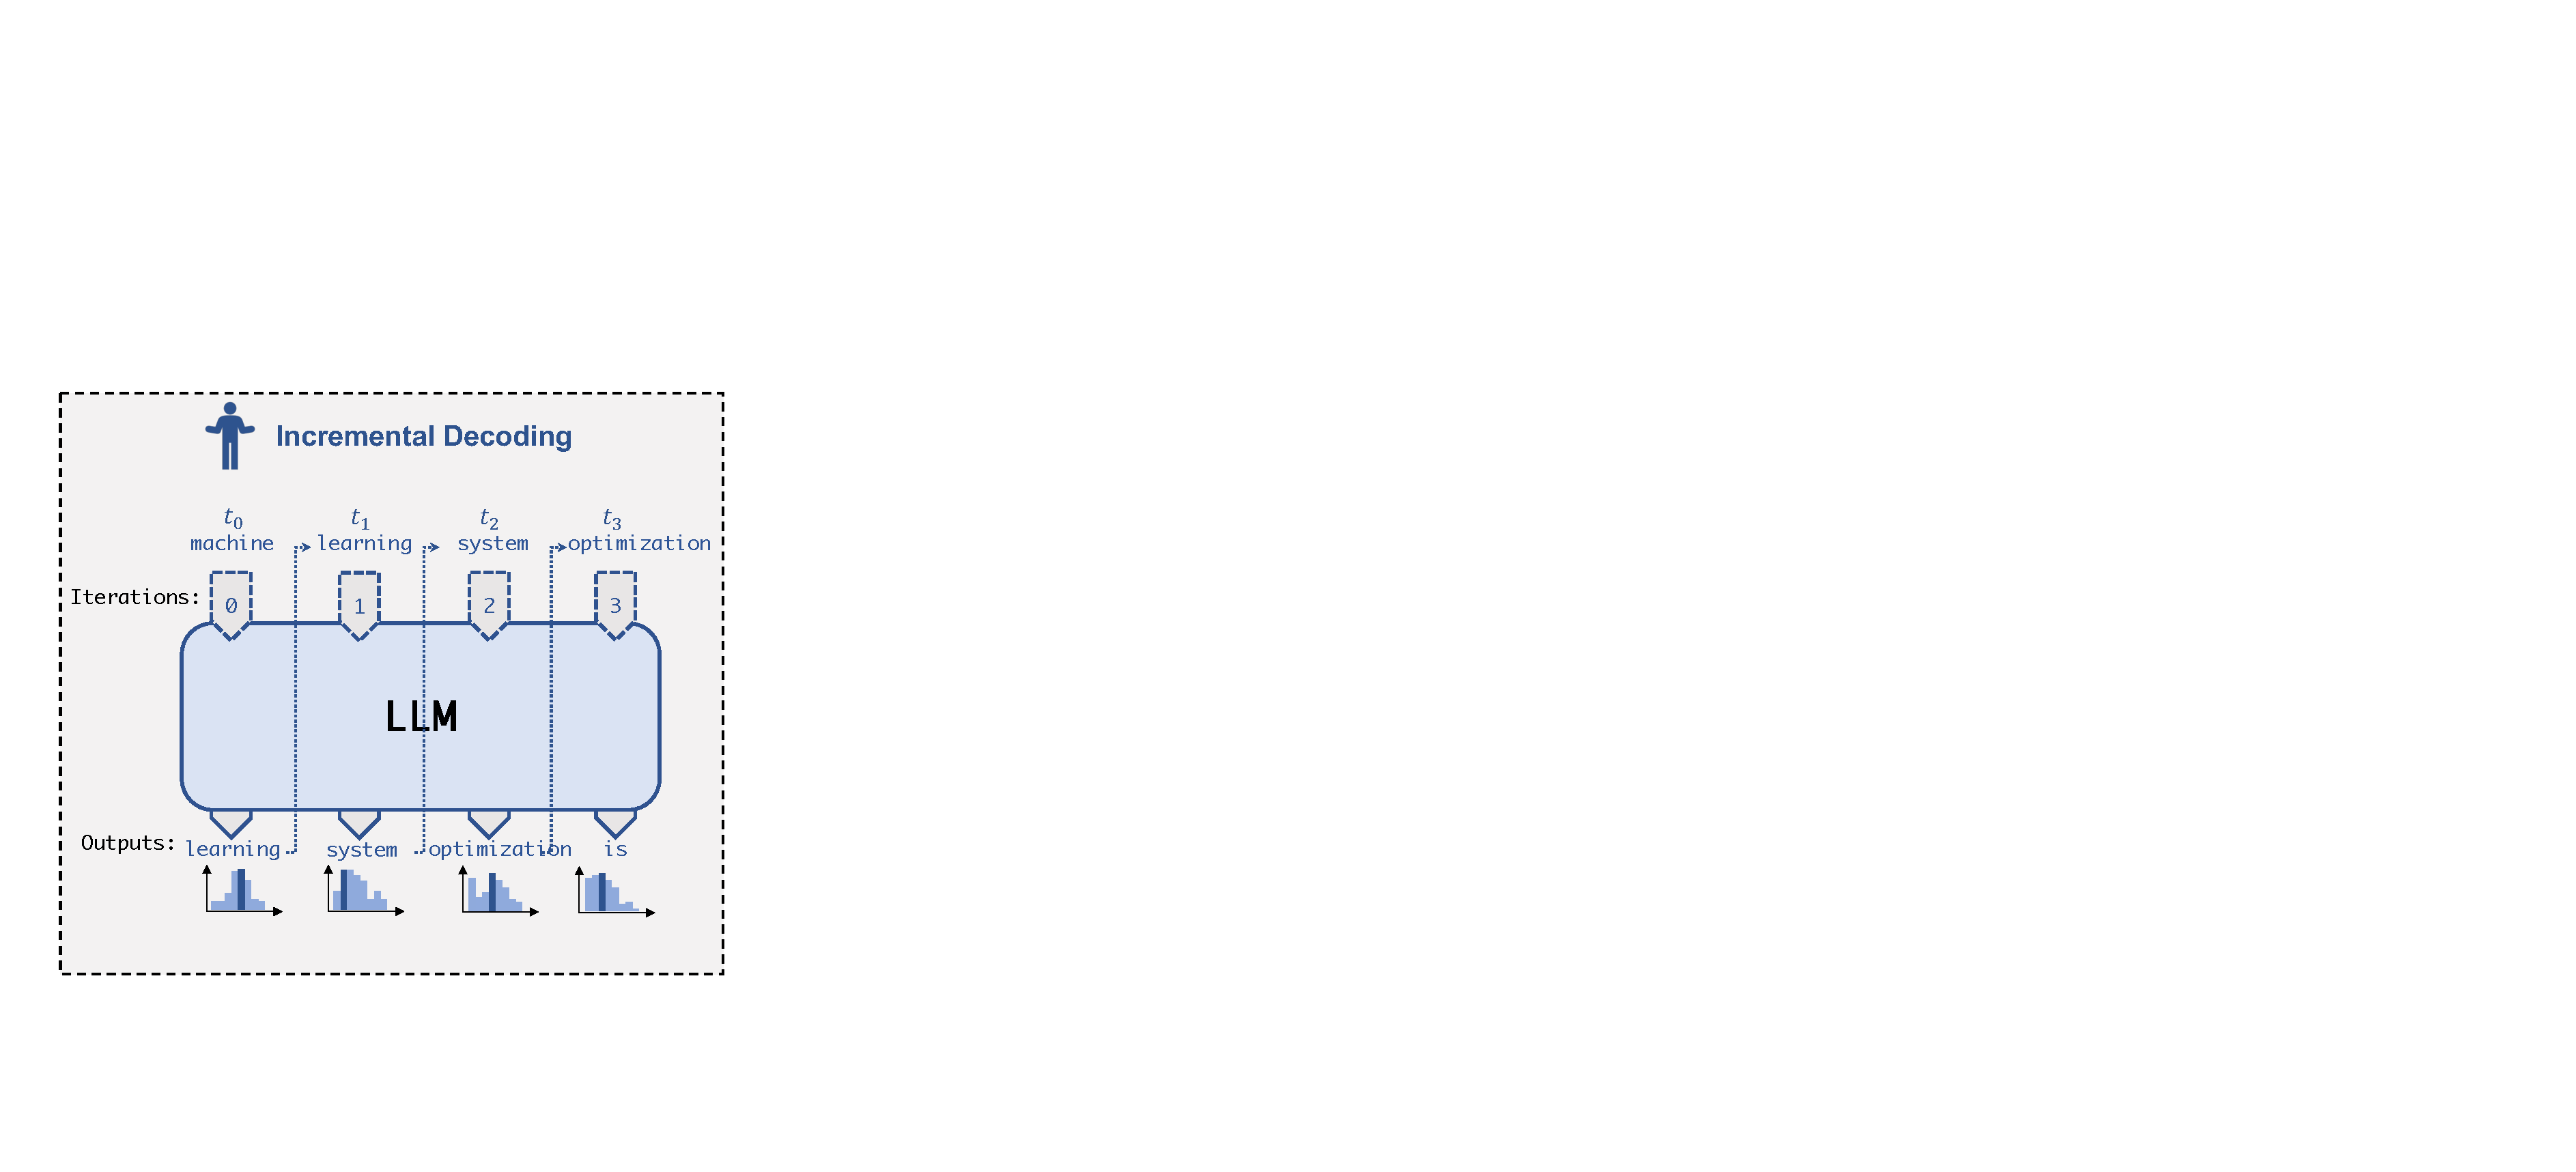
\includegraphics[width=\linewidth]{figures/specinfer/existing_overview6a4}
        \caption{Incremental decoding.}
        \label{background:fig:decoding:incremental}
    \end{subfigure}
    \hfill
    \begin{subfigure}[t]{0.56\linewidth}
        \centering
        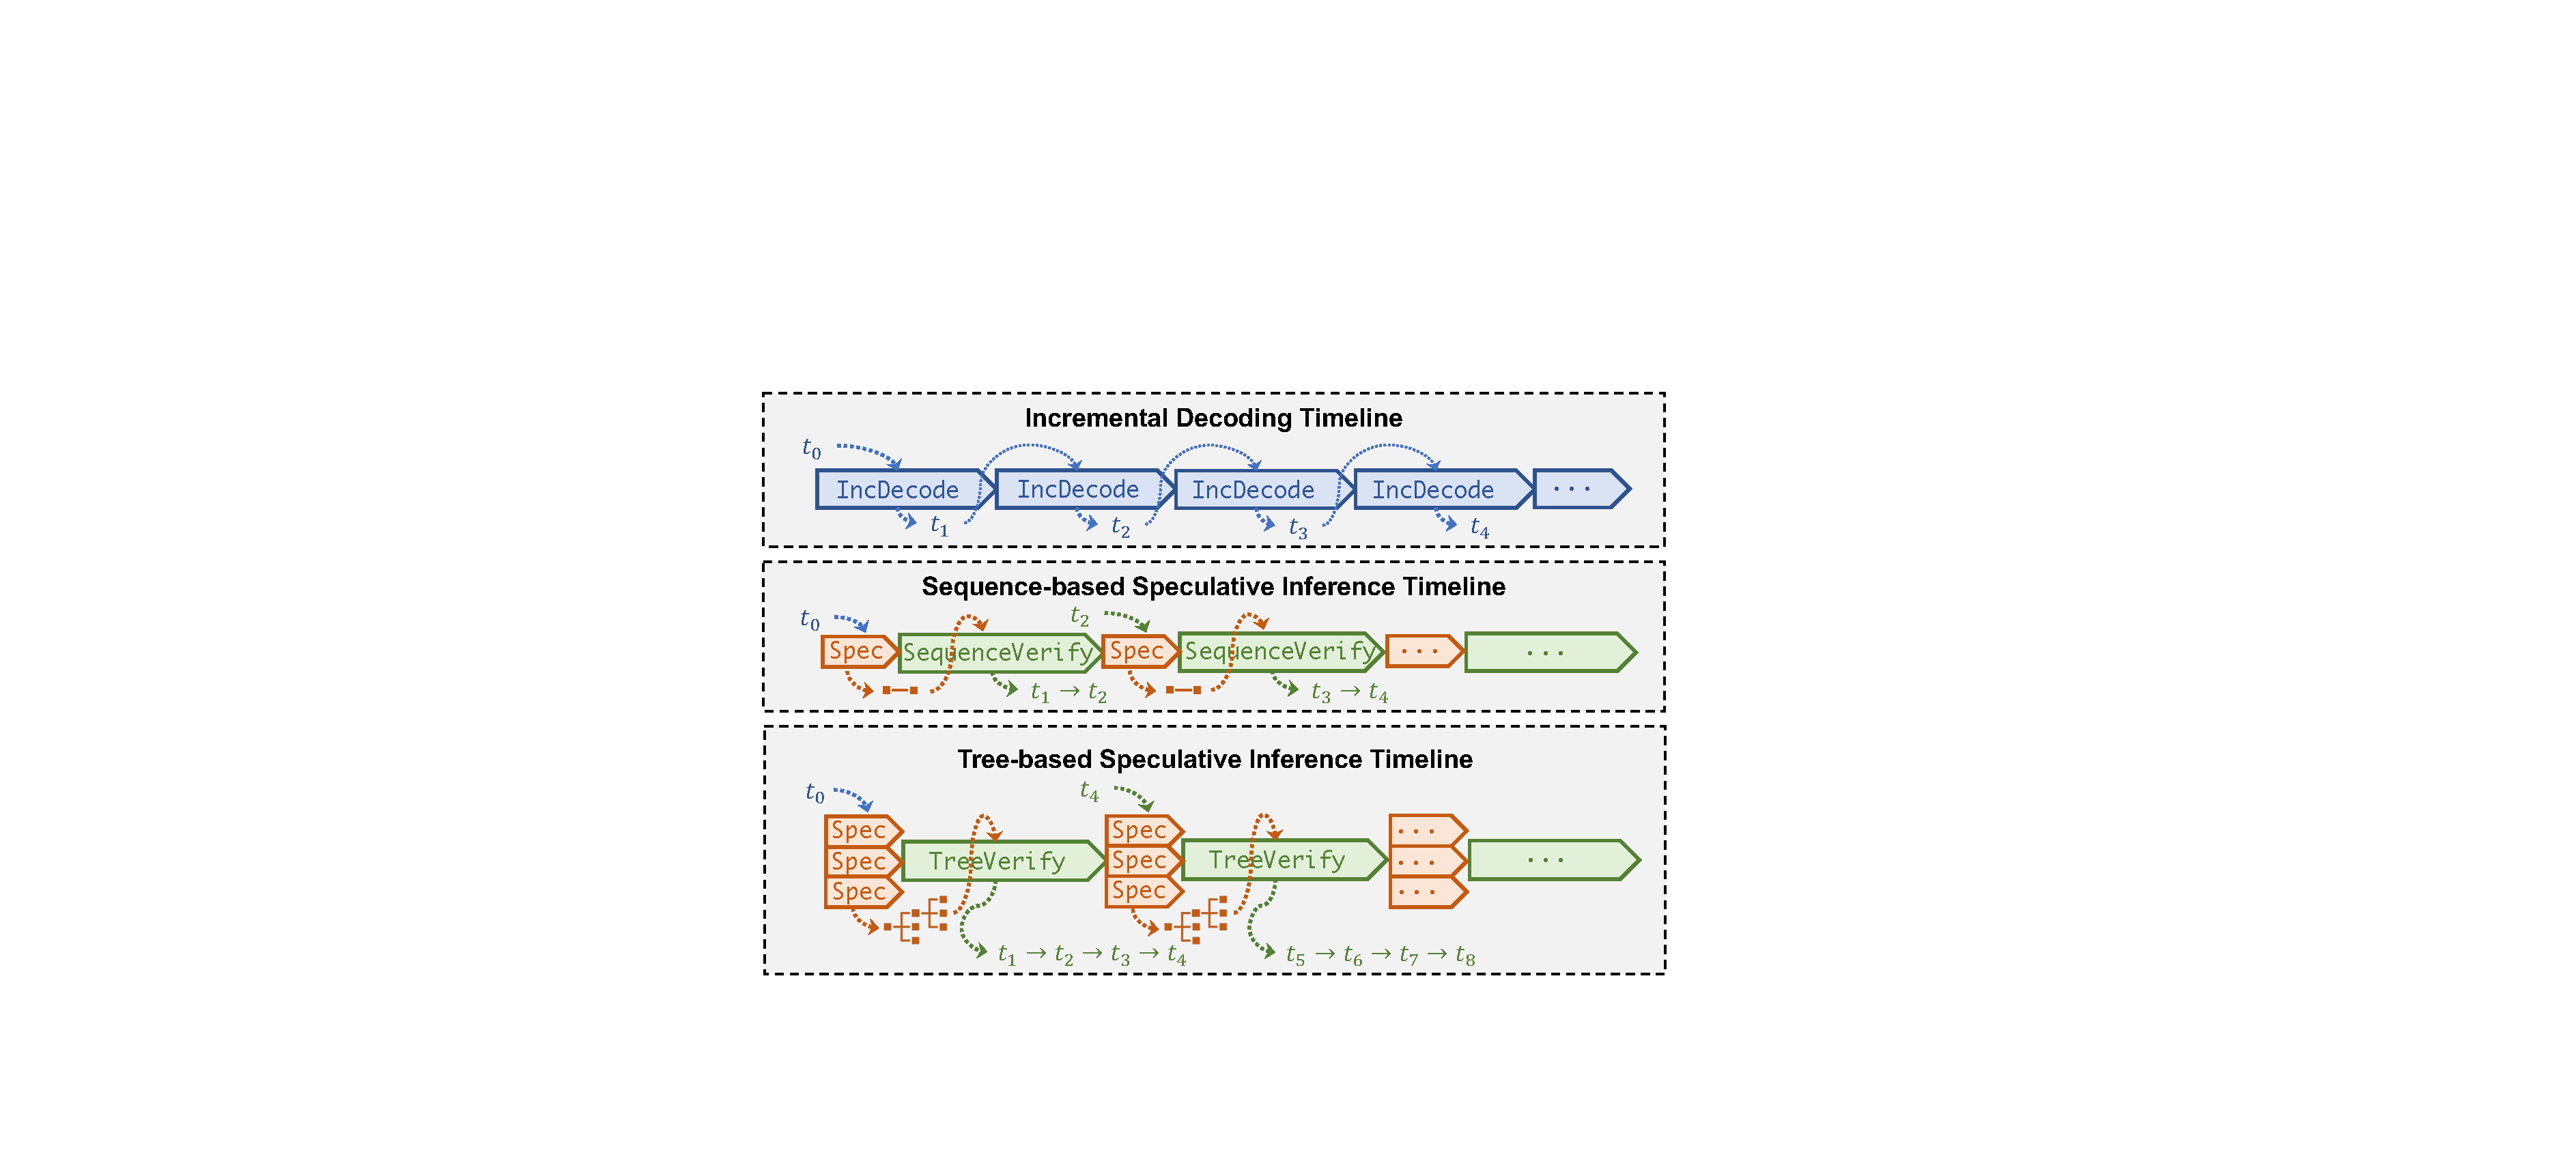
\includegraphics[width=\linewidth]{figures/specinfer/existing_overview6b6}
        \caption{Timeline comparison.}
        \label{background:fig:decoding:timeline}
    \end{subfigure}
    \caption{Incremental (autoregressive) decoding generates one token per forward pass of the LLM (a). Speculative decoding instead uses a cheap drafter to propose several tokens and verifies them against the LLM in a single pass; sequence-based speculation verifies one candidate continuation, whereas tree-based speculation, introduced in \Cref{ch:specinfer}, verifies many at once (b).}
    \label{background:fig:decoding}
\end{figure}

\paragraph{The KV cache.}
The attention output for token $t$ depends on the keys and values of all tokens $j \le t$.
Recomputing those keys and values at every decode step would make the cost of generating a sequence quadratic in its length, so all serving systems \emph{cache} the per-layer keys and values of every processed token and append to this \emph{KV cache} as generation proceeds~\cite{pope2023efficiently,vllm}.
The cache turns each decode step into a cheap operation for the model's linear layers (one new row) but makes memory the binding constraint: for a model with $L$ layers, $H_{kv}$ key-value heads of dimension $d_h$, each token occupies $2 \cdot L \cdot H_{kv} \cdot d_h$ values (keys and values) in the cache, which for a 70B-parameter model in 16-bit precision is on the order of hundreds of kilobytes per token and tens of gigabytes for a batch of long requests.
The cache is also what makes long-context and agentic workloads, whose prompts routinely run to tens of thousands of tokens (\Cref{background:sec:agents}), expensive to serve concurrently: the number of requests that fit on a GPU is bounded by the memory left after the weights, and managing that memory well is one of the main contributions of modern serving systems (\Cref{background:sec:serving}).

\subsection{Why Decoding Underutilizes GPUs}
\label{background:subsec:memory_bound}

The decode phase is \emph{memory-bandwidth bound}.
Every decode step must read all $N$ model parameters from GPU high-bandwidth memory (HBM) once, regardless of how many requests are batched together, and it performs roughly $2N$ floating-point operations per request in the batch.
With a batch of $B$ requests the arithmetic intensity of the step is therefore about $B$ operations per parameter byte read (in 16-bit precision, $B/2$ FLOPs per byte).
In the roofline model~\cite{williams2009roofline}, a kernel is compute bound only when its arithmetic intensity exceeds the ratio of peak compute to peak memory bandwidth of the device.
For an NVIDIA A100 (312 TFLOP/s of 16-bit tensor-core compute, 2 TB/s of HBM bandwidth) that ratio is about 150 FLOPs per byte, and for an H100 (roughly 1 PFLOP/s and 3.35 TB/s~\cite{nvidia2022hopper}) it is about 300.
Decode steps with batches of a few dozen requests, which is what latency targets usually allow, sit far below these ridge points: the tensor cores idle while the memory system streams weights, and the KV cache reads for long sequences add to the traffic without adding useful compute.
Prefill, with hundreds or thousands of tokens per request, sits on the other side of the ridge.

The consequence is that the latency of a decode step is close to the time to read the weights (and the KV cache) from HBM, and the GPU's compute capacity is mostly wasted during generation.
This observation is the premise of speculative decoding (\Cref{background:sec:specdec}): if a step is going to read all of the weights anyway, verifying several candidate tokens in that same step costs little more than generating one, so the ``free'' compute can be spent on checking guesses about the future~\cite{leviathan2022fast,chen2023accelerating,specinfer}.
It is also the premise of co-serving (\Cref{background:sec:peft}): the compute left idle by latency-critical decoding can be reclaimed by throughput-oriented work that shares the same weights.

\subsection{The Cost of Scale}
\label{background:subsec:cost}

Model quality has improved with scale~\cite{kaplan2020scaling,brown2020language,chowdhery2022palm}, and the cost of inference has grown with it.
GPT-3's 175 billion parameters require more than eight 40GB A100 GPUs just to hold the weights in half precision~\cite{brown2020language,zhang2022opt}; the open-weight DeepSeek-V3 has 671 billion parameters~\cite{deepseekai2024deepseekv3}; and frontier proprietary models~\cite{openai2023gpt4,gpt5} are larger still.
A single request to such a model takes seconds to serve, and a multi-GPU server costs hundreds of thousands of dollars and consumes kilowatts of power, with individual accelerators now exceeding 1,000W~\cite{lithos2025}.
Reasoning models that generate long chains of thought before answering~\cite{o1-preview,guo2025deepseek} multiply the number of decode steps per request, and agentic applications multiply the number of requests per task (\Cref{background:sec:agents}).
Serving efficiency is therefore not a second-order concern: it determines which models can be deployed at all, which applications are affordable, and how much latency a user experiences.
The systems in this thesis address this cost at three levels: by reducing the number of sequential decode steps (\Cref{ch:specinfer,ch:suffixdecoding}), by reclaiming the GPU capacity that bursty inference leaves idle (\Cref{ch:flexllm}), and by producing better kernels for the operators every step executes (\Cref{ch:fastkernels,ch:kernelseek}).

\section{LLM Serving Systems}
\label{background:sec:serving}

An LLM serving system accepts a stream of generation requests, schedules them onto one or more GPUs, and returns their outputs under latency and throughput constraints.
This section reviews the mechanisms that production systems use to do this efficiently, because they are both the foundation that the systems in this thesis are built on and the baselines they are compared against: \SpecInfer (\Cref{ch:specinfer}) is evaluated against vLLM, HuggingFace TGI, FasterTransformer, and FlexGen; \SuffixDecoding (\Cref{ch:suffixdecoding}) is implemented inside vLLM; \FlexLLM (\Cref{ch:flexllm}) is compared against dedicated vLLM inference clusters and PEFT finetuning stacks; and \FastKernels (\Cref{ch:fastkernels}) validates its measurement instrument against vLLM and SGLang before scoring any agent.

\subsection{Batching}
\label{background:subsec:batching}

Because a decode step is bandwidth bound, batching requests is the single most effective way to raise throughput: the weights are read once per step regardless of batch size, so adding a request to a batch adds compute but almost no memory traffic until the batch reaches the ridge point of \Cref{background:subsec:memory_bound}.
Early serving systems such as FasterTransformer~\cite{fastertransformer} batched at the granularity of requests, which forces the whole batch to wait for its longest member and leaves slots idle as shorter requests finish.
Orca~\cite{yu2022orca} introduced \emph{iteration-level scheduling} (now usually called \emph{continuous batching}), in which the scheduler revisits the batch at every decode step, retiring finished requests and admitting new ones immediately, together with \emph{selective batching} that batches the linear layers across requests while running attention per request.
Continuous batching is now universal: vLLM~\cite{vllm}, TGI~\cite{huggingface_tgi}, TensorRT-LLM~\cite{tensorrt-llm}, DeepSpeed-MII~\cite{deepspeed-mii}, and SGLang~\cite{sglang} all implement it.
Sarathi and Sarathi-Serve~\cite{agrawal2023sarathi,agrawal2024taming} refined it with \emph{chunked prefill}, which splits long prompts into chunks and co-schedules each chunk with the decode steps of other requests, so that a long prefill does not stall every in-flight request for an entire step.
NanoFlow~\cite{nanoflow} goes further and overlaps compute-, memory-, and network-bound operations within a single device by splitting the batch into nano-batches.
Throughout this thesis, iteration-level scheduling is the unit at which our systems make decisions: \SpecInfer and \SuffixDecoding change what one iteration verifies, and \FlexLLM changes what one iteration contains.

\subsection{Memory Management}
\label{background:subsec:memory}

With weights fixed, the KV cache determines how many requests can be batched.
vLLM's PagedAttention~\cite{vllm} applies virtual-memory ideas to this cache: instead of reserving a contiguous region sized for the maximum output length of each request, it allocates fixed-size blocks on demand and keeps a per-request block table, which eliminates most of the internal and external fragmentation of earlier systems and lets blocks be shared between requests with a common prefix (for example, parallel samples from the same prompt).
SGLang's RadixAttention~\cite{sglang} generalizes prefix sharing across requests over time by keeping the KV cache of recently served prompts in a radix tree keyed by token sequence, so that a new request that shares a prefix with an earlier one (the system prompt of a chat application, the few-shot examples of a pipeline, the accumulated transcript of an agent) skips prefill for the shared portion; SGLang pairs this with a frontend language for expressing multi-call LLM programs and a compressed finite-state machine for constrained decoding.
Prefix caching is highly relevant to the agentic workloads of \Cref{background:sec:agents}, which reuse context aggressively; \SuffixDecoding (\Cref{ch:suffixdecoding}) exploits the complementary observation that such workloads also repeat their \emph{outputs}.

\subsection{Multi-GPU Serving}
\label{background:subsec:parallelism}

Models that do not fit on one GPU, or whose latency targets cannot be met by one GPU's bandwidth, are served across several.
\emph{Tensor model parallelism}~\cite{shoeybi2020megatronlm} partitions the weight matrices of each layer across GPUs, so every GPU holds a slice of every layer and the GPUs exchange partial results with an all-reduce after each attention and FFN block; it divides the per-step weight read across devices, directly lowering decode latency, but requires fast interconnect (NVLink) and is therefore usually confined to a single node.
\emph{Pipeline parallelism}~\cite{huang2019gpipe} instead assigns contiguous groups of layers to different GPUs and streams micro-batches through them; it needs only point-to-point communication and scales across nodes, but does not reduce the latency of a single request and introduces pipeline bubbles.
Production systems combine the two, with tensor parallelism within a node and pipeline parallelism across nodes~\cite{aminabadi2022deepspeed,tensorrt-llm}, and this is also the configuration used in \SpecInfer's distributed experiments (\Cref{ch:specinfer}).
Choosing a parallelization strategy is itself an optimization problem; FlexFlow and Unity~\cite{jia2019flexflow,unger2022unity} and Alpa~\cite{zheng22-alpa} search this space automatically for training, AlpaServe~\cite{li2023alpaserve} does so for serving multiple models, and \FlexLLM extends the idea with \emph{dependent parallelization} of PEFT adapters relative to the base model they attach to (\Cref{ch:flexllm}).
More recent work disaggregates the prefill and decode phases onto separate GPU pools so that each can be provisioned and parallelized for its own profile~\cite{zhong2024distserve,patel2024splitwise}.

\paragraph{Offloading.}
At the other end of the spectrum, \emph{offloading-based} inference serves a model that does not fit in GPU memory from a single commodity GPU by keeping weights, KV cache, or both in CPU DRAM or on disk and streaming them to the GPU as needed~\cite{sheng2023flexgen,aminabadi2022deepspeed}.
FlexGen~\cite{sheng2023flexgen} formulates the placement and schedule as a linear program and reaches high throughput by processing very large batches between transfers, but each decode step still pays the cost of moving the weights over PCIe, which is an order of magnitude slower than HBM.
Offloading magnifies the memory-bound character of decoding: anything that extracts more than one token from each pass over the weights, as speculative decoding does, pays off proportionally more, which is why \SpecInfer's gains are largest in the offloading setting (\Cref{ch:specinfer}).

\subsection{Service-Level Objectives and Workloads}
\label{background:subsec:slo}

Serving systems are evaluated against \emph{service-level objectives} (SLOs) that reflect how users experience generation~\cite{zhong2024distserve,wang2024towards,adaserve}.
\emph{Time to first token} (TTFT) is the latency of prefill plus queueing; \emph{time per output token} (TPOT), or per-token latency, is the interval between successive output tokens during decode; and end-to-end latency is their combination over the length of the output.
Interactive chat tolerates a TPOT of a few tens of milliseconds, while agentic pipelines care about the end-to-end latency of an entire multi-call task (\Cref{background:sec:agents}).
Throughput, measured in requests or tokens per second, is the system-level counterpart, and \emph{goodput}, the throughput of requests that meet their SLOs, combines the two~\cite{zhong2024distserve,turbospec}.
A system can trade these against each other: larger batches raise throughput but lengthen each decode step and hence TPOT, so a latency SLO caps the usable batch size and, by \Cref{background:subsec:memory_bound}, caps GPU utilization.

Real inference traffic complicates the picture further.
Production traces show request arrivals that are bursty and non-stationary over minutes and hours, with prompt and output lengths that vary by orders of magnitude across and within applications~\cite{wang2024towards,burstgpt}.
Because the latency SLO must hold during bursts, operators provision for peaks, and the GPUs sit partially idle the rest of the time; reported average utilizations of production inference clusters are as low as 52\% at Microsoft and 10\% at Alibaba~\cite{lithos2025}.
Work on spot instances~\cite{miao2023spotserve}, fair scheduling across tenants~\cite{sheng2024fairness,aqua2024}, and SLO-aware speculation~\cite{adaserve,turbospec} all respond to this variability.
\FlexLLM (\Cref{ch:flexllm}) takes the complementary view that the idle capacity reserved for bursts should be filled by work that tolerates delay, and it does so at the granularity of individual tokens within an iteration so that it can give the capacity back the moment a burst arrives.

\section{Speculative Decoding}
\label{background:sec:specdec}

\subsection{Draft and Verify}
\label{background:subsec:draft_verify}

Speculative decoding exploits the asymmetry identified in \Cref{background:subsec:memory_bound}: an LLM can only \emph{generate} one token per forward pass, but it can \emph{verify} many.
The idea is borrowed from speculative execution in processors, where a pipeline predicts the outcome of a branch and executes ahead of it, discarding the work if the prediction turns out to be wrong~\cite{burton1985speculative,gabbay1996speculative,smith1998study,hennessy2011computer}.
In the LLM setting~\cite{stern2018blockwise,leviathan2022fast,chen2023accelerating,xiaspeculative,gante2023assisted}, a cheap \emph{drafter} proposes a sequence of $\gamma$ candidate tokens $\hat{x}_{t+1}, \ldots, \hat{x}_{t+\gamma}$ given the prefix $x_{\le t}$.
The target LLM then runs a single forward pass over the prefix extended by the candidates, which yields its next-token distribution at every one of the $\gamma + 1$ positions simultaneously, exactly as a prefill pass does.
A \emph{verifier} walks the candidates in order, accepting each token that the target model agrees with and stopping at the first disagreement; the position at which it stops also provides a correctly distributed token from the target model, so every verification step produces at least one new token and at most $\gamma + 1$.
\Cref{background:fig:decoding:timeline} contrasts this with incremental decoding.
When the drafter is cheap and its proposals are frequently accepted, the number of expensive sequential passes over the target model shrinks by the average number of accepted tokens, and because each pass reads the weights once regardless of how many positions it evaluates, the extra compute of verification is nearly free while decode stays memory bound.

\subsection{Lossless Verification}
\label{background:subsec:lossless}

What distinguishes speculative decoding from lossy acceleration techniques such as quantization or pruning~\cite{frantar2023gptq,frantar2023sparsegpt,biglittletransformer} is that it provably preserves the output distribution of the target model.
Under greedy decoding the argument is immediate: the verifier accepts a candidate only if it equals the target model's argmax at that position, so the accepted prefix is exactly what incremental greedy decoding would have produced, and the first rejected position is replaced by the target's own argmax.
Under stochastic decoding the guarantee comes from \emph{speculative sampling}~\cite{leviathan2022fast,chen2023accelerating}.
Let $p(\cdot)$ be the target distribution at a position and $q(\cdot)$ the drafter's distribution, and let $\hat{x} \sim q$ be the candidate.
The verifier accepts $\hat{x}$ with probability $\min\!\big(1, p(\hat{x})/q(\hat{x})\big)$; on rejection it samples a replacement from the residual distribution
\[
p'(x) = \frac{\max\big(0,\, p(x) - q(x)\big)}{\sum_{x'} \max\big(0,\, p(x') - q(x')\big)}
\]
and stops.
A short calculation shows that the token emitted at that position, whether accepted or resampled, is distributed exactly according to $p$, independently of $q$.
The drafter therefore affects only \emph{speed}, through how often its candidates are accepted, and never \emph{quality}; a bad drafter degrades gracefully to incremental decoding.
This property is what makes speculative decoding safe to deploy transparently in a serving system, and both \SpecInfer and \SuffixDecoding preserve it: \SpecInfer extends speculative sampling to token trees with its multi-step speculative sampling (\Cref{ch:specinfer}), and \SuffixDecoding inherits the greedy and stochastic guarantees unchanged because its drafter, though not a model, produces candidates that are verified the same way (\Cref{ch:suffixdecoding}).

\subsection{Sequence-Based and Tree-Based Speculation}
\label{background:subsec:tree}

The original formulation drafts a single sequence.
Its expected gain per step is governed by the acceptance rate $\alpha$: if each candidate is accepted independently with probability $\alpha$, the expected number of tokens per verification step is $(1 - \alpha^{\gamma+1})/(1 - \alpha)$~\cite{leviathan2022fast}, which saturates quickly for moderate $\alpha$ because a single early mistake wastes every candidate after it.
Drafters that are small enough to be cheap are often 100--1000$\times$ smaller than the target and frequently disagree with it, particularly under stochastic decoding, where even a well-aligned drafter guesses the sampled token only with the probability the target assigns to it.

\emph{Tree-based speculation}, introduced by \SpecInfer~\cite{specinfer} and adopted since by most model-based methods~\cite{cai2024medusasimplellminference,li2024eagle,eagle2,sequoia}, replaces the single draft sequence with a \emph{token tree} in which each node is a candidate token and each root-to-node path is a candidate continuation.
The tree hedges the drafter's uncertainty: where a sequence commits to one guess at every position, a tree can keep several alternatives at the positions where the drafter is unsure, so that a mistake on one branch does not forfeit the tokens on another.
Verifying a tree in one forward pass requires an attention variant that respects the tree's ancestor structure rather than a linear causal mask, a \emph{tree attention} in which each node attends only to its ancestors, plus a KV-cache layout that stores the tree's branches without duplicating their shared prefix.
\SpecInfer's tree-based parallel decoding provides exactly this, and it raises the per-token verification success rate from 52--57\% for a single sequence to 96--97\% for a tree in its stochastic-decoding experiments (\Cref{ch:specinfer}).
Later work optimizes the \emph{shape} of the tree: Sequoia~\cite{sequoia} chooses a topology for a given hardware budget, EAGLE-2~\cite{eagle2} grows the tree dynamically according to the drafter's confidence, and SLO-aware schedulers size the tree per request~\cite{adaserve}.

\subsection{Model-Based and Model-Free Drafters}
\label{background:subsec:drafters}

Drafters divide into two families according to where their predictions come from.

\paragraph{Model-based drafters} run a neural network.
The simplest is a small language model from the same family as the target, such as OPT-125M for OPT-175B or LLaMA-68M for LLaMA-65B~\cite{leviathan2022fast,chen2023accelerating,specinfer}; \SpecInfer additionally fine-tunes several such small models jointly so that their proposals cover complementary parts of the target's output (\Cref{ch:specinfer}).
Medusa~\cite{cai2024medusasimplellminference} avoids a separate model by attaching extra decoding heads to the target that predict the tokens two, three, and more positions ahead from the current hidden state.
EAGLE~\cite{li2024eagle,eagle2,li2025eagle3scalinginferenceacceleration} trains a lightweight autoregressive head on the target's hidden features rather than its tokens, which removes most of the drafter's uncertainty and currently gives the highest acceptance rates among model-based methods.
Related approaches include blockwise parallel decoding~\cite{stern2018blockwise,kim2024accelerating}, multi-token prediction heads trained into the model~\cite{gloeckle2024multitoken}, self-speculation using early exits or skipped layers of the target~\cite{draftverify,bita}, and lookahead decoding, which generates n-grams in parallel with Jacobi iteration~\cite{fu2024lookahead}.
All of them spend GPU time on the drafter at every step, and that time is not negligible: a draft head or small model must itself be executed autoregressively to produce $\gamma$ tokens, it competes with the target for the GPU, and the two must be interleaved at the kernel level~\cite{sequoia,eagle2}.

\paragraph{Model-free drafters} look the candidates up instead of computing them.
Prompt lookup decoding~\cite{saxena2023prompt} searches the current prompt for the most recent occurrence of the last few generated tokens and proposes whatever followed it; LLMA~\cite{yang2023inference} does the same against retrieved reference documents, REST~\cite{he2024rest} against a datastore built from a corpus, Token Recycling~\cite{luo2024turningtrashtreasureaccelerating} against the target model's own recent top-$k$ predictions, and ANPD~\cite{ou2024losslessaccelerationlargelanguage} against an adaptive n-gram model of the prefix.
These drafters cost microseconds on the CPU and leave the GPU entirely to the target model, so their overhead is negligible; their acceptance rate, however, depends on how much of the output is literally present in their reference text.
In open-ended conversation this is little, and model-free methods lose to model-based ones; in workloads that copy, edit, or regenerate existing text, such as code editing and the agentic pipelines of \Cref{background:sec:agents}, long runs of output are predictable from context and lookup-based drafting can accept dozens of tokens at a time.
The methods above also typically speculate a \emph{fixed} number of tokens regardless of how likely they are to be accepted, which wastes verification compute when the match is weak.

\subsection{The Acceptance-Overhead Tradeoff}
\label{background:subsec:tradeoff}

The speedup of any speculative method is governed by two quantities: the expected number of accepted tokens per step, which depends on the drafter's alignment with the target and on the shape and length of the speculation, and the per-step overhead, which includes the drafter's own cost, the extra verification compute (significant once batches approach the ridge point, since verifying $\gamma + 1$ positions per request multiplies the batch's token count), and the serving system's orchestration.
Model-based drafters buy acceptance with overhead; model-free drafters have almost no overhead but only speculate well on repetitive text.
Longer speculation raises the ceiling but lowers the acceptance of the trailing tokens, and the optimal length shrinks as the batch grows~\cite{turbospec}.
A good speculative decoding system therefore has to be \emph{adaptive}: it should speculate aggressively when it is confident and conservatively otherwise, and it should fall back to incremental decoding when neither is warranted.

\paragraph{Positioning.}
\SpecInfer (\Cref{ch:specinfer}) is the model-based, tree-structured point in this design space: it introduces token trees and tree-based parallel decoding, shows how to build trees from one or several small speculative models, and proves that tree verification remains lossless under stochastic decoding.
\SuffixDecoding (\Cref{ch:suffixdecoding}) is the model-free point, specialized for agentic workloads: it drafts from suffix trees over the prompt and over previous outputs, uses frequency statistics in those trees to score candidates and to decide \emph{how far} to speculate at each step, and can hand over to a model-based drafter when the trees have nothing to offer.
Both leave the target model's output distribution untouched.

\section{Parameter-Efficient Finetuning and LLM Platforms}
\label{background:sec:peft}

\subsection{Finetuning as a Service}
\label{background:subsec:finetuning_service}

Pretraining an LLM is expensive enough that almost no organization does it, and a small number of foundation models are instead adapted to many downstream uses by \emph{finetuning}: continued training on a task-specific dataset~\cite{devlin2018bert,radford2019language,brown2020language,houlsby2019parameter,zhang2021share}.
Demand for finetuning comes from the need to customize models to a domain or style~\cite{liu2024customizing}, to train on private data without sharing it~\cite{tan2024democratizing}, and to keep models current as data changes~\cite{gao2023unified}.
Every major LLM platform therefore offers a finetuning API alongside its inference API~\cite{openaifinetuning,googlefinetuning,databricksfinetuning}, and open-source toolkits make the same workflow available on self-hosted clusters~\cite{peft,llamafactory,transformers}.
From the operator's point of view this creates two workloads with opposite characteristics over the same models: inference is latency-critical, bursty, and submitted by users one request at a time, whereas finetuning is throughput-oriented, tolerant of delays of minutes to hours, and submitted as a whole dataset at once.

\subsection{Parameter-Efficient Finetuning}
\label{background:subsec:peft_methods}

Full finetuning updates every parameter and so requires, per model copy, the memory for the weights, their gradients, and the optimizer state, several times the memory of inference~\cite{kingma2014adam}.
\emph{Parameter-efficient finetuning} (PEFT) methods~\cite{ding2023parameter} instead freeze the pretrained weights and train a small number of new or selected parameters.
Adapters~\cite{houlsby2019parameter,pfeiffer2020adapterfusion} insert small bottleneck layers between the frozen ones; prefix and prompt tuning~\cite{li2021prefix,lester2021power,liu2023gpt} learn virtual tokens prepended to the input or to each layer's keys and values; (IA)$^3$~\cite{liu2022few} learns per-dimension scaling vectors; and unified frameworks combine these by heuristics or architecture search~\cite{he2021towards,mao2021unipelt,zhou2023autopeft}.
The dominant method is \emph{low-rank adaptation} (LoRA)~\cite{hu2021lora}, which represents the update to a weight matrix $W \in \mathbb{R}^{d \times k}$ as the product of two low-rank factors, $W + BA$ with $B \in \mathbb{R}^{d \times r}$, $A \in \mathbb{R}^{r \times k}$, and $r \ll \min(d, k)$; the trainable parameters shrink by orders of magnitude, no new inference latency is introduced if $BA$ is merged into $W$, and QLoRA~\cite{dettmers2023qlora} extends the recipe to a 4-bit quantized base model so that large models can be finetuned on a single GPU.
PEFT reduces trainable parameters and optimizer state dramatically, but it does not by itself reduce the \emph{activation} memory of backpropagation, which training systems retain for every layer in order to compute gradients; \FlexLLM shows that for PEFT specifically, much of that activation memory is unnecessary because the frozen weights need no gradient, and it prunes the corresponding dependencies from the backward graph (\Cref{ch:flexllm}).

Two properties of PEFT matter for this thesis.
First, every finetuning job over a given base model, and every inference request against that base model or any of its finetuned variants, executes the \emph{same frozen forward computation}; the variants differ only in a small adapter applied on the side.
Second, the adapters are small enough that many of them can be resident on one GPU at the same time.
Together these make it possible to batch work from different adapters, and from different kinds of jobs, through a single copy of the base model.

\subsection{Multi-Adapter Serving}
\label{background:subsec:multi_adapter}

Serving systems have exploited the first property for inference.
PetS~\cite{zhou2022pets} decouples each linear layer into a shared base operation and small task-specific operations so that requests for different adapters share the base computation.
Punica~\cite{chen2023punica} introduces a segmented gather-matrix-vector CUDA kernel that applies different LoRA adapters to different requests within one batch, and S-LoRA~\cite{sheng2023s} adds unified paging of adapter weights and KV cache together with heterogeneous batching to serve thousands of adapters from one GPU.
dLoRA~\cite{wu2024dlora} dynamically switches between merged and unmerged adapter execution and migrates requests across replicas, Chameleon~\cite{iliakopoulou2024chameleon} caches and schedules adapters adaptively, and reports from practice show hundreds of task-specific LoRA models rivaling much larger general models at a fraction of the serving cost~\cite{zhao2024lora}.
These systems share base weights across inference requests for different adapters; \FlexLLM extends sharing in the other direction, across inference and \emph{finetuning} of adapters, where the forward pass is identical but the finetuning side also needs a backward pass.

\subsection{Separate Clusters and GPU Sharing}
\label{background:subsec:gpu_sharing}

Despite this sharing opportunity, the prevailing deployment pattern runs inference and finetuning on \emph{separate, dedicated clusters}, each with a system specialized for its workload~\cite{weng2022mlaas,gao2022deep,chen2023deepboot}.
The inference cluster is provisioned for peak load to protect its SLOs, and by \Cref{background:subsec:slo} it is underutilized most of the time; the finetuning cluster, meanwhile, cannot touch that idle capacity.
Reclaiming it requires sharing GPUs between the two workloads, and the systems literature offers three broad mechanisms~\cite{yu2022survey}.
\emph{Temporal sharing} time-slices a GPU between jobs; Gandiva~\cite{xiao2018gandiva} and AntMan~\cite{xiao2020antman} apply it to deep-learning training clusters, and PipeSwitch~\cite{bai2020pipeswitch} and PREMA~\cite{choi2020prema} reduce the cost of switching and preempting.
Time slicing lets each job use the whole GPU, but an inference request that arrives during a finetuning slice must wait for the slice to end, which is incompatible with millisecond latency targets unless the slices are very short, in which case switching overhead and the loss of batching dominate.
\emph{Spatial sharing} runs kernels from different jobs concurrently on disjoint subsets of the GPU's streaming multiprocessors, via multiple CUDA streams, NVIDIA's Multi-Process Service (MPS)~\cite{mps}, or the hardware partitioning of Multi-Instance GPU (MIG)~\cite{mig}; GSLICE~\cite{dhakal2020gslice}, Gpulet~\cite{choi2022serving}, and MuxFlow~\cite{zhao2023muxflow} build schedulers on top of these.
Spatial partitions, however, are coarse and slow to reconfigure (MIG partitions in particular cannot be resized without draining the GPU~\cite{migpartition}), so a partition sized for normal inference load fails during a burst while one sized for the burst wastes resources the rest of the time; and because the two jobs' kernels remain separate, each reads the shared base weights from HBM independently.
Across all of these mechanisms, prior work has found that co-locating training with inference degrades inference latency unless the system is carefully designed around it~\cite{romero2021infaas,choi2022serving}.

\paragraph{Positioning.}
\FlexLLM (\Cref{ch:flexllm}) introduces a fourth mechanism, \emph{co-serving}, that is specific to LLMs and PEFT.
Because inference requests and PEFT finetuning jobs over the same base model execute the same frozen forward computation, \FlexLLM fuses them at the granularity of individual tokens within one iteration-level batch: finetuning tokens ride along in the same GPU kernels as inference tokens, the weights are read once for both, and a token-level scheduler decides at every iteration how many finetuning tokens to admit given the current inference load and its SLO.
Reallocation therefore happens at the millisecond timescale of an iteration rather than at the timescale of a time slice or a partition change, which is what allows the system to absorb inference bursts without violating SLOs while filling the troughs with finetuning.

\section{Agentic LLM Workloads}
\label{background:sec:agents}

\subsection{What Agents Are}
\label{background:subsec:agents_def}

An \emph{agentic} application does not issue a single prompt and return a single completion; it decomposes a task into many LLM calls whose inputs depend on the outputs of earlier calls and on the results of actions taken in an environment.
The building blocks are by now well established.
Chain-of-thought prompting~\cite{wei2022chain} has the model reason step by step before answering, and reasoning models train this behavior in~\cite{o1-preview,guo2025deepseek}.
ReAct~\cite{yao2023react} interleaves reasoning with \emph{tool use}: the model emits an action (a search query, a shell command, a function call), the harness executes it and appends the observation to the context, and the model continues.
\emph{Self-consistency}~\cite{wang2023selfconsistencyimproveschainthought} samples several reasoning paths for the same prompt and votes; \emph{self-refinement} and Reflexion~\cite{madaan2023selfrefine,shinn2023reflexion} have the model critique and revise its own output over several rounds; decomposed prompting~\cite{khot2023decomposedpromptingmodularapproach} splits a task into subtasks handled by specialized prompts; and \emph{multi-agent} frameworks~\cite{wu2023autogen,chen2024autoagentsframeworkautomaticagent,wang2024mixtureofagentsenhanceslargelanguage} assign roles to several model instances that exchange messages.
Retrieval-augmented generation~\cite{gao2024retrievalaugmentedgenerationlargelanguage,wang2024speculativeragenhancingretrieval} adds retrieved documents to the context of some or all calls.
A production pipeline such as the AgenticSQL system evaluated in \Cref{ch:suffixdecoding} composes several of these: a classification call, parallel candidate-generation calls, a merge call, and refinement calls, all for one user question.

\paragraph{Software-engineering agents.}
The most demanding and most studied agentic workload is software engineering.
Given a repository and an issue description, an agent must navigate the code, reproduce the problem, edit files, run tests, and iterate until the tests pass.
SWE-bench~\cite{jimenez2024swebenchlanguagemodelsresolve} made this measurable with real GitHub issues and their test suites, and a succession of agents has driven resolution rates up: SWE-agent~\cite{yang2024sweagent} showed that the design of the agent-computer interface (how files are viewed, searched, and edited) matters as much as the model; CodeAct and OpenHands~\cite{wang2024executablecodeactionselicit,openhands} let the agent act by writing and executing code; Agentless~\cite{xia2024agentless} showed that a fixed localize-repair-validate pipeline is competitive with free-form agents; and commercial harnesses such as Claude Code and Codex~\cite{anthropic2025claudecode,codex} now run such loops at scale.
An agent of this kind issues tens to hundreds of LLM calls for one task, each with the accumulated transcript of previous calls in its context, and each separated from the next by the execution of a tool.

\subsection{Why Agents Stress Serving Systems}
\label{background:subsec:agents_stress}

Agentic workloads differ from chat in ways that invalidate several assumptions of the systems in \Cref{background:sec:serving}.

\paragraph{Many dependent calls.}
A task is not done until its last call returns, and the calls are sequentially dependent, so per-call latency accumulates: a pipeline of 50 dependent calls at 2 seconds each takes nearly two minutes regardless of throughput.
Per-token decode latency, which chat tolerates because humans read slowly, becomes the dominant term in end-to-end task time, which is what \Cref{ch:suffixdecoding} measures.
Systems such as Parrot~\cite{lin2024parrot}, ALTO~\cite{10.1145/3642970.3655844}, and Autellix~\cite{luo2025autellix} expose the structure of the program to the serving system so that it can schedule across calls, pipeline between agents, and prioritize calls on the critical path, and Dynasor~\cite{fu2024efficientlyservingllmreasoning} terminates reasoning paths early once their outcome is certain.

\paragraph{Long contexts.}
Each call carries the transcript so far: the system prompt, tool definitions, the issue, every file the agent has viewed, and every command output.
Contexts of tens of thousands of tokens are routine, so the KV cache of \Cref{background:subsec:autoregressive} grows large, prefill is repeated for mostly-unchanged prompts unless prefix caching (\Cref{background:subsec:memory}) catches it, and the number of concurrent agents a GPU can host shrinks.

\paragraph{Heavy repetition.}
Consecutive calls of an agent overlap not only in their prompts but in their \emph{outputs}.
A self-refinement loop rewrites a document while changing a few lines; a coding agent regenerates a function with one fix; a multi-agent pipeline produces structured outputs with the same schema and boilerplate every time; self-consistency samples share long stretches of reasoning; and SWE-bench agents repeatedly emit near-identical commands, file paths, and edit blocks.
This repetition is invisible to a model-based drafter, which must rediscover it token by token, but it is exactly what a model-free drafter can exploit.
Measured as the empirical entropy of the next token given a short context, agentic outputs are far more predictable than open-ended chat (\Cref{ch:suffixdecoding}).

\paragraph{Positioning.}
\SuffixDecoding (\Cref{ch:suffixdecoding}) targets this workload directly: it treats the outputs of earlier calls as a cache for drafting the outputs of later ones, maintains that cache in suffix trees that grow with the workload, and adapts its speculation length to how well the current context matches history, which pays off most on the long repeated runs that agents produce.
Agentic workloads also motivate the second half of this thesis in a different way.
The same coding agents that stress serving systems are now capable of writing systems code themselves, including the GPU kernels that serving systems depend on (\Cref{background:sec:kernelagents}).
\Cref{ch:fastkernels,ch:kernelseek} ask how well they do so under production conditions and how they should be steered when the kernel is hard.

\section{GPU Kernels for Machine Learning}
\label{background:sec:gpu}

\subsection{The GPU Execution Model}
\label{background:subsec:gpu_model}

Every operator in \Cref{background:sec:llm}, and every scheduling decision in \Cref{background:sec:serving,background:sec:peft}, ultimately executes as a sequence of GPU \emph{kernels}: functions launched over a grid of thread blocks, each block running on one of the GPU's \emph{streaming multiprocessors} (SMs)~\cite{nvidia2025cudaguide}.
An NVIDIA H100 has 132 SMs and a B200 has 148~\cite{nvidia2022hopper,nvidia2024blackwell}.
Threads execute in \emph{warps} of 32 that issue instructions in lockstep; a block's warps share a fast, software-managed \emph{shared memory} (up to 228KB per SM on Hopper) and a large register file, and the SM's warp schedulers hide latency by switching among resident warps.
The memory hierarchy below that is a shared L2 cache (50MB on H100) and HBM, whose bandwidth, 3.35TB/s on H100 and about 8TB/s on B200, is the resource that decode-phase kernels are bound by (\Cref{background:subsec:memory_bound}).
\emph{Tensor cores} perform dense matrix multiply-accumulate on small tiles at throughputs an order of magnitude above the general-purpose cores; on Hopper they are driven by warp-group-level asynchronous instructions (\texttt{wgmma}) whose operands live in shared memory, and on Blackwell by a new generation (\texttt{tcgen05}) that accumulates into a dedicated tensor memory, with cluster-level multicast and lower-precision formats added in each generation~\cite{nvidia2022hopper,nvidia2024blackwell}.
Hopper also introduced the \emph{Tensor Memory Accelerator} (TMA), which copies tiles between HBM and shared memory asynchronously, and thread-block clusters that let SMs share data through distributed shared memory.
Each of these features is exposed to the programmer, and each must be used explicitly to reach the hardware's peak.

\subsection{What Makes a Kernel Fast}
\label{background:subsec:kernel_fast}

The roofline model~\cite{williams2009roofline} gives the first-order answer: a kernel is limited either by memory bandwidth or by compute, and a fast kernel for a memory-bound operator moves the minimum number of bytes while a fast kernel for a compute-bound operator keeps the tensor cores busy.
Getting there involves a small set of recurring techniques, and the difficulty is in composing them.
\emph{Tiling} partitions the output into blocks sized so that the operands of each block fit in shared memory and registers, so that each byte loaded from HBM is reused many times; the choice of tile shape trades reuse against parallelism and register pressure.
\emph{Fusion} merges consecutive operators into one kernel so that intermediates never round-trip through HBM; FlashAttention~\cite{flashattention} is the canonical example, computing softmax attention tile by tile with an online normalization so that the $n \times n$ attention matrix is never materialized, which turns attention from memory bound to compute bound and makes long contexts feasible.
\emph{Occupancy}, the number of warps resident per SM, must be high enough to hide memory and pipeline latency but is capped by the registers and shared memory each block consumes.
\emph{Coalescing} arranges each warp's memory accesses to fall in contiguous, aligned segments so that one transaction serves 32 threads; tensor layouts in shared memory must additionally be \emph{swizzled} to avoid bank conflicts.
\emph{Overlap} keeps the memory system and the tensor cores busy simultaneously through software pipelining, multi-stage buffers, and, on recent GPUs, \emph{warp specialization}, in which producer warps issue asynchronous TMA loads while consumer warps run tensor-core instructions, synchronized through barrier phases~\cite{shah2024flashattention3}.
\emph{Persistent} kernels launch one block per SM that loops over work items, which amortizes launch cost and enables cross-tile scheduling, and on the host side, launch overhead, CUDA-graph capture, and the shape of the dispatch path can matter as much as the kernel body when the operator is small~\cite{hu2024korch,jin2026eventtensor}.
Public worklogs that take a matrix multiplication from a naive kernel to cuBLAS parity on Ampere, Hopper, and Blackwell~\cite{boehm2022cudammm,shankhdhar2024h100,modular2025blackwell} illustrate how many of these steps are needed and how the right sequence changes from one generation to the next.

\subsection{Programming Layers}
\label{background:subsec:programming_layers}

Kernels are written at several levels of abstraction, and the level determines how much of the machinery above the programmer controls.
At the bottom, CUDA C++~\cite{nvidia2025cudaguide} exposes threads, shared memory, and (through PTX intrinsics) every hardware feature; it offers the highest ceiling and the most ways to be wrong.
CUTLASS and its CuTe layout algebra~\cite{nvidia2023cutlass} provide templated building blocks for tiled GEMM-like kernels on NVIDIA tensor cores, and ThunderKittens~\cite{spector2025thunderkittens} offers a smaller set of tile primitives with the same goal; both encode hardware-specific best practices that would otherwise be rediscovered per kernel, at the cost of large compile-time template surfaces and dependence on the library tracking each new GPU.
Triton~\cite{triton} raises the level to blocked programs in a Python DSL whose compiler handles memory coalescing, shared-memory allocation, and tensor-core instruction selection; it is the default path for custom kernels in PyTorch and the language most kernel-generation benchmarks target (\Cref{background:sec:kernelagents}).
Above that, compilers generate kernels from the model graph: PyTorch's \texttt{torch.compile}~\cite{ansel2024pytorch2,paszke2019pytorch} captures Python bytecode and lowers it through Inductor to Triton, TVM and Ansor~\cite{chen2018tvm,zheng2020ansor} search over loop schedules, and graph-level optimizers such as TASO, PET, and Mirage~\cite{jia2019taso,wang2021pet,wu2025mirage} search over algebraic rewrites of the computation, with Mirage extending the search into the kernel and thread-block levels.
Finally, hand-optimized libraries sit alongside these: cuBLAS and cuDNN~\cite{nvidia2025cublas,nvidia2025cudnn} for dense linear algebra and convolution, and for LLM serving specifically, FlashAttention and its successors~\cite{flashattention,dao2024flashattention2,shah2024flashattention3,zadouri2026flashattention4}, FlashInfer~\cite{ye2025flashinfer}, and the kernels shipped inside vLLM, SGLang, and TensorRT-LLM~\cite{vllm,sglang,tensorrt-llm}.
The kernels a production serving system actually runs are drawn from the top of this stack, and any new kernel, whether written by a person or an agent, must beat them to be worth deploying; this is the baseline \FastKernels measures against (\Cref{ch:fastkernels}).

\subsection{Hardware Churn and Emerging Operators}
\label{background:subsec:churn}

The tradeoffs above are not stable across GPU generations.
Each generation changes the tensor-core instruction set, the memory hierarchy, and the asynchronous machinery, so the best kernel for an operator must be rewritten.
Attention is the clearest case~\cite{miao2023towards}: FlashAttention on Ampere~\cite{flashattention,dao2024flashattention2} was followed by FlashAttention-3 on Hopper~\cite{shah2024flashattention3}, built around warp specialization, \texttt{wgmma}, TMA, and pingpong scheduling to overlap softmax with matrix multiplication, and then by FlashAttention-4 on Blackwell~\cite{zadouri2026flashattention4}, rebuilt again around \texttt{tcgen05} and tensor memory; each rewrite reported a 1.5--2$\times$ speedup over its predecessor on the new hardware, and each took an expert team months.
The same holds for GEMM, where even NVIDIA's own libraries sit well below the hardware's speed of light on many production shapes~\cite{solexecbench}, and the gap widens for operators that are not GEMMs.
The emerging operators of \Cref{background:subsec:transformer}, MoE routing and expert dispatch, linear-attention and state-space scans, gated delta rules, low-bit quantized GEMMs, speculative-decoding verification over token trees, and multimodal preprocessing, arrive in new models faster than hand-written kernels can follow, so they are typically served first by generic PyTorch implementations or by \texttt{torch.compile} output, at a fraction of attainable performance.
Production serving stacks therefore live in a permanent state of kernel debt: at any moment, some operators on some hardware have mature kernels and others do not, and the set changes every time a model family or a GPU is released.
This churn is the concrete form that the thesis statement's premise takes at the kernel layer, and it is what motivates using agents to write kernels.

\section{LLM Agents for Code and Kernel Generation}
\label{background:sec:kernelagents}

\subsection{Coding Agents and Harnesses}
\label{background:subsec:coding_agents}

LLMs trained on code~\cite{chen2021evaluating} became useful for software engineering once they were placed in a \emph{harness}: a loop that lets the model read and edit files, run compilers and tests, observe the results, and try again~\cite{yang2024sweagent,openhands,anthropic2025claudecode,codex}.
How the harness is built changes what the same model can do.
The agent-computer interface of SWE-agent~\cite{yang2024sweagent} and the minimal pipeline of Agentless~\cite{xia2024agentless} both improved results by changing what the model sees rather than the model itself; practitioner guidance favors simple, composable loops over elaborate scaffolds~\cite{anthropic2024effectiveagents}; and giving the model too many tools or too much context has measurable costs~\cite{langchain2025toolload,liu2024lost}.
A parallel literature documents how LLMs behave as optimizers over long horizons: they search greedily from their priors~\cite{redko2026priorknowledge}, anchor on the solution in the prompt~\cite{jones2022cognitivebiases}, explore poorly without intervention~\cite{krishnamurthy2024explore}, stop early after a run of failures~\cite{merouani2025compilot}, lock in to early decisions under iterative refinement~\cite{javaji2025turnwise}, and report success that the environment contradicts~\cite{advani2026falsesuccess}.
Intrinsic self-correction helps less than one would hope~\cite{huang2024cannotselfcorrect,sharma2024sycophancy}, whereas external feedback on a model's own code, particularly feedback that proposes structural changes the model did not consider, substantially raises repair success~\cite{olausson2024selfrepair,wang2024hypothesissearch}.
These findings frame the design question of \Cref{ch:kernelseek}: what should a human, or a harness, supply to a coding agent working on a hard optimization target.

\subsection{Kernel-Generation Benchmarks}
\label{background:subsec:kernel_benchmarks}

GPU kernels are an attractive target for coding agents because the goal is objective (the output must match a reference and run faster), the feedback is cheap (compile, test, time), and the expertise is scarce (\Cref{background:subsec:churn}).
KernelBench~\cite{kernelbench} established the evaluation format: a PyTorch reference module, a set of input shapes, and a score combining correctness and speedup over the reference, organized into levels from single operators to whole models drawn from an earlier generation of architectures.
Successors broadened the surface, with TritonBench and CUDABench~\cite{tritonbench,cudabench} for specific languages, BackendBench and MultiKernelBench~\cite{backendbench,multikernelbench} for more backends, KernelCraft, ComputeEval, and NPUEval~\cite{kernelcraft,nvidia2025computeeval,kalade2025npueval} for emerging hardware and robustness, FlashInfer-Bench~\cite{flashinferbench,xing2026flashinferbench} and KSearch~\cite{cao2026ksearch} for serving kernels inside an inference engine, SOL-ExecBench~\cite{solexecbench} for production shapes scored against speed-of-light bounds, and CommBench and ParallelKernelBench~\cite{commbench,parallelkernelbench} for multi-GPU communication.

The first generation of benchmarks also revealed systematic weaknesses.
Their inputs are synthetic, usually random tensors of fixed shape, so kernels are never tested on the data-dependent behavior (MoE routing skew, ragged batches, paged caches) that dominates in production.
Their baselines are weak: speedup over eager PyTorch, or at best \texttt{torch.compile}, is easy to obtain and says little about whether the kernel beats what vLLM or SGLang already ship.
Their scoring is vulnerable to \emph{reward hacking}: agents have learned to exploit loose numerical tolerances, timing harness quirks, caching across runs, and reference implementations that can be bypassed, which robust-kbench and KernelBench-Verified~\cite{robustkbench,zhang2026kernelbenchverified} document and partially repair.
And their tasks are isolated: a kernel is scored alone, on one GPU, behind a simplified interface, so a benchmark win need not survive integration into the compilation stacks, interfaces, and end-to-end execution paths of a real serving system.

\subsection{Kernel-Generation Agents}
\label{background:subsec:kernel_agents}

Agents for these benchmarks span a \emph{structure-freedom} axis.
\emph{Scripted} agents fix what the model does at each step: a generate-test-refine loop with a policy trained by reinforcement learning on kernel rewards (Kevin, CUDA-L1, KernelLLM, AutoTriton, QiMeng, DrKernel, CUDA-Agent~\cite{baronio2025kevin,li2025cudal1,kernelllm2025,li2025autotriton,zhu2026qimeng,drkernel,cudaagent2026}), a menu of optimizations keyed to profiler diagnostics (Autocomp, KernelPro~\cite{hong2025autocomp,kernelpro2026}), or a team of agents with fixed roles for planning, coding, profiling, and review (Astra, KernelAgent, CudaForge, GEAK, KDA, AKO, and others~\cite{wei2025astra,kernelagent,cudaforge,wang2025geak,kda,han2026kda,ako,kernelskill2026,luo2026houmao,sun2026kernelclaw}).
These are sample-efficient but encode what to try, and they fail where the script is wrong: Autocomp collapses without its menu~\cite{hong2025autocomp}, and RL loops competitive on single operators fail on fused models~\cite{drkernel,zhu2026qimeng,cudaagent2026}.
\emph{Open-ended} agents use the LLM as the mutation operator of an \emph{evolutionary search} over a population of programs, in the lineage of FunSearch and AlphaEvolve~\cite{romeraparedes2024funsearch,alphaevolve} and continued by OpenEvolve, ShinkaEvolve, EvoEngineer, CUCo, KernelFoundry, and TTT-Discover~\cite{openevolve,lange2025shinkaevolve,guo2025evoengineer,cuco2026,wiedemann2026kernelfoundry,yuksekgonul2026tttdiscover}; AVO~\cite{chen2026avo} makes a self-directed coding agent the variation operator, and Meta and Cursor with NVIDIA run such loops across whole kernel libraries~\cite{liao2025kernelevolve,kernelevolve,cursor2026multiagent}.
The freedom buys headline results, including gains over FlashAttention-4 and over AlphaEvolve's own FlashAttention baseline~\cite{chen2026avo,alphaevolve}, and is paid for in trials: hundreds of explored directions over days, a large fraction of incorrect candidates~\cite{guo2025evoengineer,cuco2026}, and edits that undo earlier edits~\cite{pelleriti2026evotrace}.
Orthogonal to this axis is how much the agent is \emph{equipped}: tool-rich agents hand the model parsed profiler output, documentation retrieval, reference implementations, and persistent knowledge stores~\cite{chen2026avo,han2026kda}, while minimal agents give it a shell and a goal.
The evidence that equipment is what is missing is weak; profiler and compiler output rarely supply the specific hypothesis the model lacks~\cite{redko2026priorknowledge}, and in the MLSys 2026 FlashInfer kernel contest, agents given expert direction beat the same agents running autonomously on every kernel~\cite{mlsys26contest,shui2026harness}.

\paragraph{Positioning.}
\FastKernels (\Cref{ch:fastkernels}) addresses the benchmark side.
It derives its tasks top-down from real model architectures so that every task has a production counterpart, matches the interfaces of the production modules so that generated kernels can be deployed as-is, captures real inputs so that data-dependent operators are tested on data they will see, scores candidates against the kernels production frameworks ship rather than against PyTorch, and evaluates every candidate end to end inside the model it came from, where interface mismatches and composition failures surface.
Its seed evaluation shows that kernel-level success barely predicts deployment, which is the gap the benchmark exists to measure.
\KernelSeek (\Cref{ch:kernelseek}) addresses the agent side for deep targets such as FlashAttention-class kernels, where whole-pipeline choreography rather than local edits determines performance.
It keeps the freedom of an open-ended coding agent, equips it minimally with a harness that verifies correctness and timing against a seed kernel, and supplies \emph{direction} at decision points through questions that name a hypothesis without giving an answer; the questions that recur harden into a bank the agent applies to itself, and the whole composes with evolutionary search.

\section{Summary}
\label{background:sec:summary}

The thread running through this chapter is that each layer of the LLM serving stack has an efficiency problem whose solution has historically required scarce expertise, and that each layer is moving.
Autoregressive decoding underutilizes GPUs because it is memory bound (\Cref{background:sec:llm}), and serving systems have developed elaborate batching, memory-management, and parallelization machinery around that fact (\Cref{background:sec:serving}).
Speculative decoding turns the idle compute into parallel verification without changing the model's outputs, and the design space of drafters and tree shapes is where \SpecInfer (\Cref{ch:specinfer}) and \SuffixDecoding (\Cref{ch:suffixdecoding}) sit (\Cref{background:sec:specdec}).
Finetuning and inference over shared frozen base models could share GPUs, but the available sharing mechanisms are too coarse for bursty, latency-critical inference, which \FlexLLM (\Cref{ch:flexllm}) resolves at token granularity (\Cref{background:sec:peft}).
Agentic applications multiply the calls, lengthen the contexts, and repeat the outputs that serving systems must handle, which \SuffixDecoding exploits, and the same agents are becoming capable of writing systems code (\Cref{background:sec:agents}).
At the bottom of the stack, GPU kernels determine the performance of every operator, and every new GPU generation and every new operator reopens the question of how to write them (\Cref{background:sec:gpu}); LLM agents are the newest tool for answering it, but the benchmarks that evaluate them have not reflected production, and the agents themselves struggle on deep targets (\Cref{background:sec:kernelagents}), which \FastKernels (\Cref{ch:fastkernels}) and \KernelSeek (\Cref{ch:kernelseek}) respectively address.
In each case, the thesis's response is the same: use smaller models, workload history, feedback-driven runtimes, or coding agents to automate an optimization that expert-only workflows cannot keep up with, while preserving the correctness guarantees and service-level objectives that production deployments require.

\chapter{\SpecInfer: Tree-Based Speculative Inference and Verification}
\label{ch:specinfer}

% TODO: adapt from reference/papers/specinfer

\chapter{\FlexLLM: Co-Serving LLM Inference and Finetuning}
\label{ch:flexllm}

% Chapter-local macros (adapted from the FlexLLM paper sources).
\providecommand{\flexllmLeftComment}[1]{\Statex \(\triangleright\) #1}

Finetuning large language models (LLMs) is essential for task adaptation, yet today's serving stacks isolate inference and finetuning on separate GPU clusters, wasting resources and under-utilizing hardware. This chapter introduces \FlexLLM, the first system to {\em co-serve} LLM inference and PEFT-based finetuning on shared GPUs by fusing computation at the token level. \FlexLLM's static compilation optimizations, {\em dependent parallelization} and {\em graph pruning}, significantly shrink activation memory, leading to end-to-end GPU memory savings of up to 80\%. At runtime, a novel {\em token-level finetuning} mechanism paired with a hybrid token scheduler dynamically interleaves inference and training tokens within each co-serving iteration, meeting strict latency SLOs while maximizing utilization. In end-to-end benchmarks on LLaMA-3.1-8B, Qwen-2.5-14B, and Qwen-2.5-32B, \FlexLLM maintains inference SLO compliance at up to 20 req/s, and improves finetuning throughput by $1.9$--$4.8\times$ under heavy inference workloads and $2.5$--$6.8\times$ under light loads, preserving over 76\% of peak finetuning progress even at peak demand. \FlexLLM is publicly available at \url{https://flexllm.github.io}.

\section{Introduction}
\label{flexllm:sec:intro}
%
Recent advancements in large language models (LLMs) such as GPT-5~\cite{gpt5,openai2023gpt4}, DeepSeek-R1~\cite{guo2025deepseek}, LLaMA-4~\cite{touvron2023llama,llama3,llama4} and Qwen~3~\cite{qwen2025qwen25technicalreport,yang2025qwen3technicalreport}, have shown strong capabilities of generating natural language texts across various application domains~\cite{zhang2019pretraining,liu2021makes,stiennon2020learning,dosovitskiy2020image}.
%
Given the increasingly high cost of LLM pre-training, there is a trend of standardizing foundational pre-trained LLMs and sharing sub-models across multiple downstream tasks~\cite{houlsby2019parameter,zhang2021share} through finetuning (i.e., continuous training on small task-specific datasets). For example, a series of {\em parameter-efficient finetuning} (PEFT) techniques~\cite{houlsby2019parameter,li2021prefix,pfeiffer2020adapterfusion,hu2021lora,he2021towards,lester2021power} have been proposed to update a subset of trainable parameters from an LLM or introduce a small number of new parameters into the LLM while keeping the vast majority of the original LLM parameters frozen. The base LLM sharing paradigm provides opportunities to multiplex resources and improve cluster utilization (e.g., Google~\cite{barham2022pathways}, Microsoft~\cite{hu2021lora}, and Tencent~\cite{nie2023angel}).
Many recent efforts~\cite{zhou2022pets,wu2024dlora,sheng2023s,chen2023punica,zhao2024lora,iliakopoulou2024chameleon} have been inspired by these opportunities to build multi-task serving systems, handling inference requests for multiple fine-tuned LLMs simultaneously in a single GPU cluster.

In addition to inference, almost all LLM serving companies (including OpenAI GPT-4o~\cite{openaifinetuning}, Google Gemini~\cite{googlefinetuning}, and Databricks Mosaic AI~\cite{databricksfinetuning}), now offer commercial finetuning APIs to facilitate the creation of custom models.
This trend is not only due to the widespread adoption of LLMs but also driven by the growing demand for task-specific model customization~\cite{liu2024customizing}, data access control~\cite{tan2024democratizing}, and the need for continuous and frequent model updating~\cite{gao2023unified}.

Currently, the most popular way to offer both inference and finetuning services is to run each task on separate, {\em dedicated} clusters~\cite{weng2022mlaas,gao2022deep,chen2023deepboot}, which exclusively use hardware resources through specialized systems optimized primarily for latency and throughput, respectively. While straightforward, this practice leads to significant economic inefficiencies. In particular, resources must be overprovisioned for inference tasks, as real-world LLM inference workloads exhibit highly unpredictable, bursty request arrival patterns~\cite{wang2024towards}. For example, public reports from Microsoft and Alibaba cite average GPU utilization rates of just 52\%~\cite{lithos2025} and 10\%~\cite{lithos2025}, respectively, with production services showing similar underutilization patterns. While inference tasks must be provisioned for peak burst capacity to maintain SLOs, the resulting idle resources during normal operation cannot be utilized by finetuning tasks, which could tolerate the latency variations (minutes to hours vs. milliseconds). This is economically unsustainable given the high cost and power demands of modern GPUs, which can now exceed 1,000W per chip~\cite{lithos2025}.

In this chapter, we explore a key research question: {\em Can we design a system that {\em simultaneously} serves both inference and finetuning tasks within a shared GPU cluster, dynamically adapting to unpredictable burst patterns while maintaining strict inference SLOs?}
Previous attempts (\Cref{flexllm:sec:coserving}) at multiplexing inference and finetuning tasks, while successful in increasing the GPU utilization, have seen limited adoption due to their impracticality.

To solve this fundamental challenge, we introduce \textit{co-serving}, a novel multiplexing technique that effectively handles bursty workloads while satisfying strict SLOs. We built \FlexLLM, the first system for LLM inference and finetuning that implements this technique. \FlexLLM introduces a \textit{PEFT-as-a-service (PaaS)} interface, which unifies inference and finetuning tasks, enabling their joint execution on shared GPU resources.
The key insight behind co-serving is that inference and finetuning tasks, when using the same base LLMs, can be merged at fine granularity---at the level of individual tokens rather than entire requests or kernels. This token-level scheduling enables millisecond-scale resource reallocation in response to inference bursts.

This co-serving approach offers critical advantages for handling bursty workloads. When inference requests suddenly spike, \FlexLLM can instantly throttle finetuning tokens within the same GPU kernel execution, reallocating resources to maintain inference SLOs without the overhead of context switching or reconfiguration. During normal load, finetuning tasks opportunistically consume the idle capacity reserved for bursts, improving overall utilization. Since the base LLM parameters are shared and frozen during finetuning, memory overhead is minimized, enabling efficient multiplexing.

Overall, this chapter makes the following key contributions:
\begin{itemize}
\item We introduce \FlexLLM, the first system to co-serve LLM inference and PEFT finetuning on shared GPUs through token-level computation fusion.
\item We develop static optimizations that reduce GPU memory requirements by up to 80\% through dependent parallelization and graph pruning.
\item We propose token-level finetuning with hybrid scheduling that maintains strict latency SLOs while maximizing GPU utilization.
\item We achieve 1.9$-$4.8$\times$ finetuning throughput improvements under heavy loads and 2.5$-$6.8$\times$ under light loads.
\end{itemize}

\section{Background and Challenges}
\label{flexllm:sec:background}
\subsection{Parameter-Efficient Finetuning}
\label{flexllm:subsec:peft}
Finetuning enables LLMs to adapt to specific domains and downstream tasks~\cite{devlin2018bert,radford2019language,brown2020language}. However, full finetuning introduces significant computational and memory overheads. To address this, {\em parameter-efficient finetuning} (PEFT) methods~\cite{ding2023parameter} have been proposed.
%
These include prompt embeddings~\cite{liu2023gpt,li2021prefix,lester2021power}, adapter modules, low-rank decomposition (LoRA)~\cite{hu2021lora}, and (IA)$^3$ \cite{liu2022few} scaling of the pre-trained weights. Recent unified approaches also combine various PEFT methods using heuristics \cite{he2021towards} or neural architecture search \cite{zhou2023autopeft,zoph2016neural,mao2021unipelt}. While PEFT approaches minimize trainable parameters, reducing parameter count is sometimes not enough to reduce the memory footprint.

\begin{figure}[htbp]
    \centering
    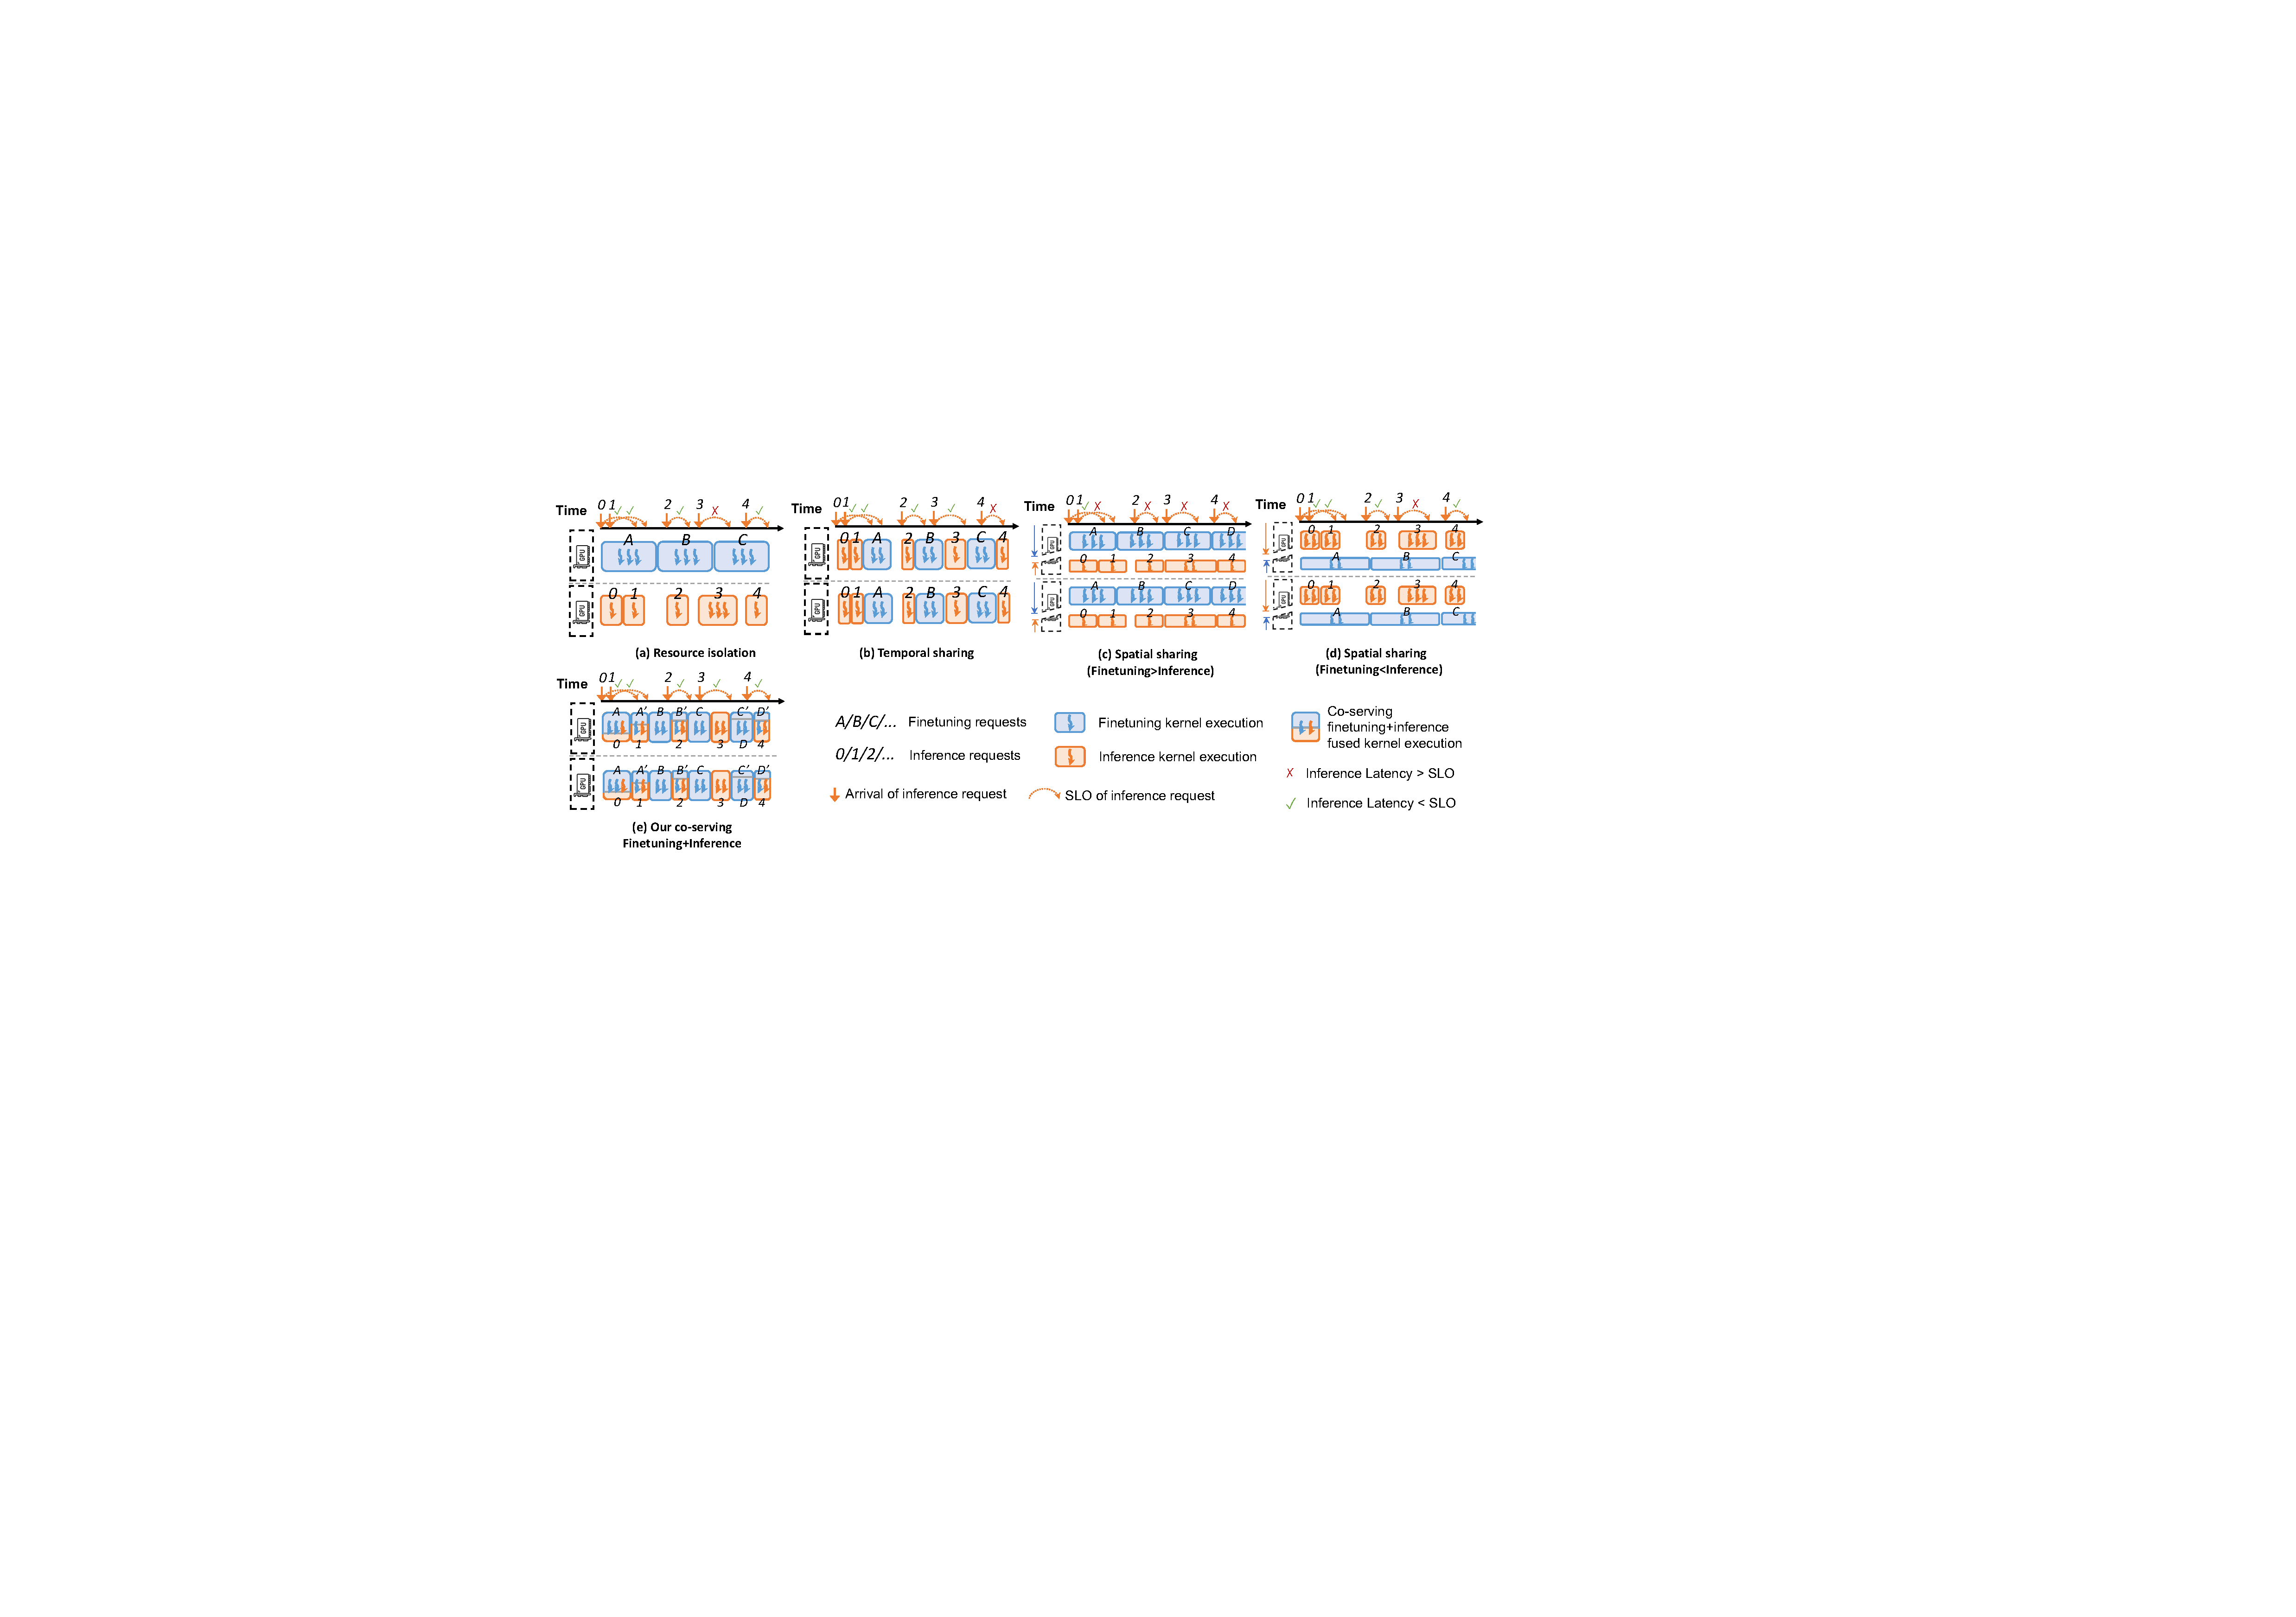
\includegraphics[width=\linewidth]{figures/flexllm/baseline7.pdf}
    \caption{Comparing different resource sharing approaches for serving finetuning and inference. For spatial sharing and co-serving, the height of rounded rectangles illustrates the splitting ratio of GPU resources (e.g., streaming multi-processors).}
    \label{flexllm:fig:baseline}
\end{figure}

\subsection{PEFT-based LLM Inference}
\label{flexllm:subsec:llm_serving}

LLM inference is increasingly essential in research and industrial applications. Recent systems serve multiple PEFT-based LLMs simultaneously. For example, PetS~\cite{zhou2022pets} decouples linear layers into shared and task-specific operations, optimizing scheduling for improved throughput.
%
More recent works focus on optimizations that are specific to generative decoding models. Punica~\cite{chen2023punica} introduces specialized CUDA kernels for multi-tenant LoRA serving. S-LoRA~\cite{sheng2023s} proposes unified paging and heterogeneous batching for thousands of LoRA components. dLoRA~\cite{wu2024dlora} improves efficiency through dynamic batching adjustments.

\subsection{Challenges in Co-serving Inference and Finetuning}
\label{flexllm:subsec:challenges}
Co-serving inference and finetuning tasks within a single system, as envisioned by \FlexLLM, presents significant challenges due to their differing workload characteristics. \FlexLLM must address three key challenges.

First, \emph{how can inference and finetuning tasks be co-located while minimizing the memory footprint}?
Traditional multi-tenancy ML scheduling systems share resources across tasks and models~\cite{xiao2018gandiva}, but suffer from the high memory demands associated with LLMs.
Furthermore, existing finetuning systems usually retain all intermediate activations similar to training systems to enable gradient computation during backpropagation, which substantially increases their resource consumption compared to pure inference tasks. This discrepancy makes it challenging to manage system resources between finetuning and inference tasks.

\FlexLLM addresses this by co-locating finetuning and inference tasks to share backbone LLM parameters and activation buffers, using {\em dependent parallelization} to optimize the placement of trainable {\em bypass networks} (e.g., LoRA adapters~\cite{hu2021lora}) in a distributed fashion (see \Cref{flexllm:subsec:parallelization}) and {\em graph pruning} to eliminate unnecessary data dependencies for frozen parameters (see \Cref{flexllm:subsec:pruning}). These optimizations reduce finetuning memory overhead by up to 8$\times$.

Next, \emph{how can we run inference and finetuning tasks simultaneously while minimizing the interference with inference latency and SLO attainment}?
Previous work on traditional ML workloads~\cite{romero2021infaas} has shown that co-locating inference with training can significantly degrade inference performance.
Unlike conventional training workloads that require coarse-grained temporal or spatial resource sharing~\cite{choi2022serving}, LLM finetuning provides a unique opportunity to batch base LLM computation and parameter access across requests from different finetuned variants~\cite{wu2024dlora}. However, due to differences in execution logic---auto-regressive decoding in inference versus backpropagation in finetuning---merging the two types of tasks remains difficult.
%
To overcome this challenge, \FlexLLM introduces {\em token-level finetuning}, decomposing finetuning sequences into smaller units (\Cref{flexllm:subsec:incremental_finetuning}) that, during the forward pass, follow the same execution order as inference tokens. In this way, both inference and finetuning tokens can be processed together using fused GPU kernels. For the backward pass, \FlexLLM launches separate GPU streams for finetuning tokens and adopts a layer-wise execution strategy to minimize memory usage.

Finally, \emph{how can we handle fluctuating inference workloads while preserving their latency SLO}?
%
Given the dynamic nature of inference request arrival patterns, provisioning for peak demand often results in significant resource under-utilization.
\FlexLLM's fine-grained, token-level execution strategy enables quick adaptation to load fluctuations.
To achieve this, \FlexLLM introduces a {\em hybrid token scheduler} (\Cref{flexllm:subsec:scheduler}) that prioritizes inference tokens for SLO compliance while opportunistically inserting finetuning tokens in a best-effort manner to maximize GPU utilization.

\section{Co-serving LLM Inference and PEFT}
\label{flexllm:sec:coserving}

Previous studies have proposed different methods for scheduling heterogeneous workloads (in our case, inference and PEFT) on shared GPU resources. These methods can be classified into three categories: \textit{resource isolation}, \textit{temporal sharing}, and \textit{spatial sharing}.
%
This section discusses the limitations inherent to these conventional approaches when applied to co-serving LLM inference and PEFT. It also highlights the fundamental distinctions between \FlexLLM's co-serving solution and previous work.
\Cref{flexllm:fig:baseline} depicts the GPU execution timelines associated with different scheduling approaches for managing inference and finetuning tasks.

\paragraph{Resource isolation.}
A common approach to support both inference and finetuning tasks is \textit{resource isolation}, which partitions the available GPUs into two distinct groups, each dedicated to handling one type of workload (see \Cref{flexllm:fig:baseline}(a)).
This approach ensures that throughput-intensive finetuning tasks do not interfere with latency-critical inference tasks.
When finetuning an LLM, a dataset of requests is provided to train the PEFT layers, with all requests submitted to \FlexLLM simultaneously, making it easier to build larger batches that can be processed sequentially. In contrast, inference requests are submitted independently by users who expect timely processing within predetermined SLOs, with the arrival times of these requests unpredictable.

Resource isolation can introduce significant GPU under-utilization, particularly in scenarios with variable request arrival rates. This is because finetuning and inference requests cannot be batched together if the number of pending requests of either type is insufficient to fully utilize a batch. With fewer GPUs available to parallelize inference computations, it may not be possible to serve requests fast enough to meet their SLO (e.g., request $r_3$ in \Cref{flexllm:fig:baseline}(a)).

\paragraph{Temporal sharing.}
Compared to resource isolation, \textit{temporal sharing}~\cite{xiao2018gandiva,xiao2020antman} improves GPU utilization by allowing different tasks to share GPU resources through time slices of different lengths depending on various parameters.
This method allows both inference and finetuning requests to access all GPUs within the cluster in turns, as shown in \Cref{flexllm:fig:baseline}(b). By using all GPUs to parallelize computation (e.g., with data parallelism or tensor model parallelism), the latency for each request can be significantly reduced, thus aiding in meeting inference SLOs. For example, while inference request $r_3$ fails to complete in the scenario illustrated in \Cref{flexllm:fig:baseline}(a) due to resource limitations, it successfully executes in \Cref{flexllm:fig:baseline}(b) by leveraging more resources. However, the arrangement of time slices can also be harmful because of the unpredictable arrival times of inference requests, which may have a stringent latency requirement that cannot be met (e.g., $r_4$ has been delayed in \Cref{flexllm:fig:baseline}(b) by pre-scheduled finetuning requests).

\paragraph{Spatial sharing.}
%
\textit{Spatial sharing} offers an alternative by enabling simultaneous execution of different tasks at the kernel level, where each task utilizes a specific portion of the GPU resources (i.e., streaming multi-processors).
%
This can be implemented on NVIDIA GPUs through multi-stream programming or by utilizing the Multi-Process Service (MPS)~\cite{mps}. Furthermore, on the latest Hopper and Ampere architectures, spatial sharing benefits from the Multi-Instance GPU (MIG)~\cite{mig}, which allows for dynamic adjustments of GPU partition configurations.
%
However, these adjustments often lack the flexibility and efficiency required to handle dynamic inference workloads effectively~\cite{dhakal2020gslice,yu2022survey,migpartition}. \Cref{flexllm:fig:baseline}(c) and (d) show two scenarios where a substantial portion of GPU resources is allocated to either finetuning or inference tasks.
%
While over-provisioning for inference tasks may appear to provide better SLO guarantees, it still falls short during peak demand periods such as the unexpected urgent request $r_3$. Additionally, over-provisioning wastes resources and significantly slows down the finetuning process.
Therefore, relying solely on spatial sharing to manage finetuning and inference tasks often results in suboptimal performance~\cite{choi2022serving,zhao2023muxflow}.

\paragraph{\FlexLLM's co-serving approach.}
As shown in \Cref{flexllm:fig:baseline}(e), \FlexLLM employs a co-serving approach that uses a fine-grained scheduling mechanism to adaptively manage both inference and finetuning requests.

Unlike temporal or spatial sharing approaches, which schedule GPU kernels of existing systems independently, \FlexLLM integrates inference and finetuning kernels. This integration reduces the overhead associated with kernel launches and minimizes accesses to GPU device memory to retrieve model weights.
%
In each iteration, \FlexLLM dynamically adjusts the allocation of inference and finetuning tokens, strategically balancing the need to meet the SLOs of inference requests with the goal of maximizing GPU utilization. This adaptive approach ensures that \FlexLLM adheres to the requirements of inference requests while optimizing the use of available GPU resources.

\section{System Overview}
\label{flexllm:sec:overview}

\begin{figure}[htbp]
    \centering
    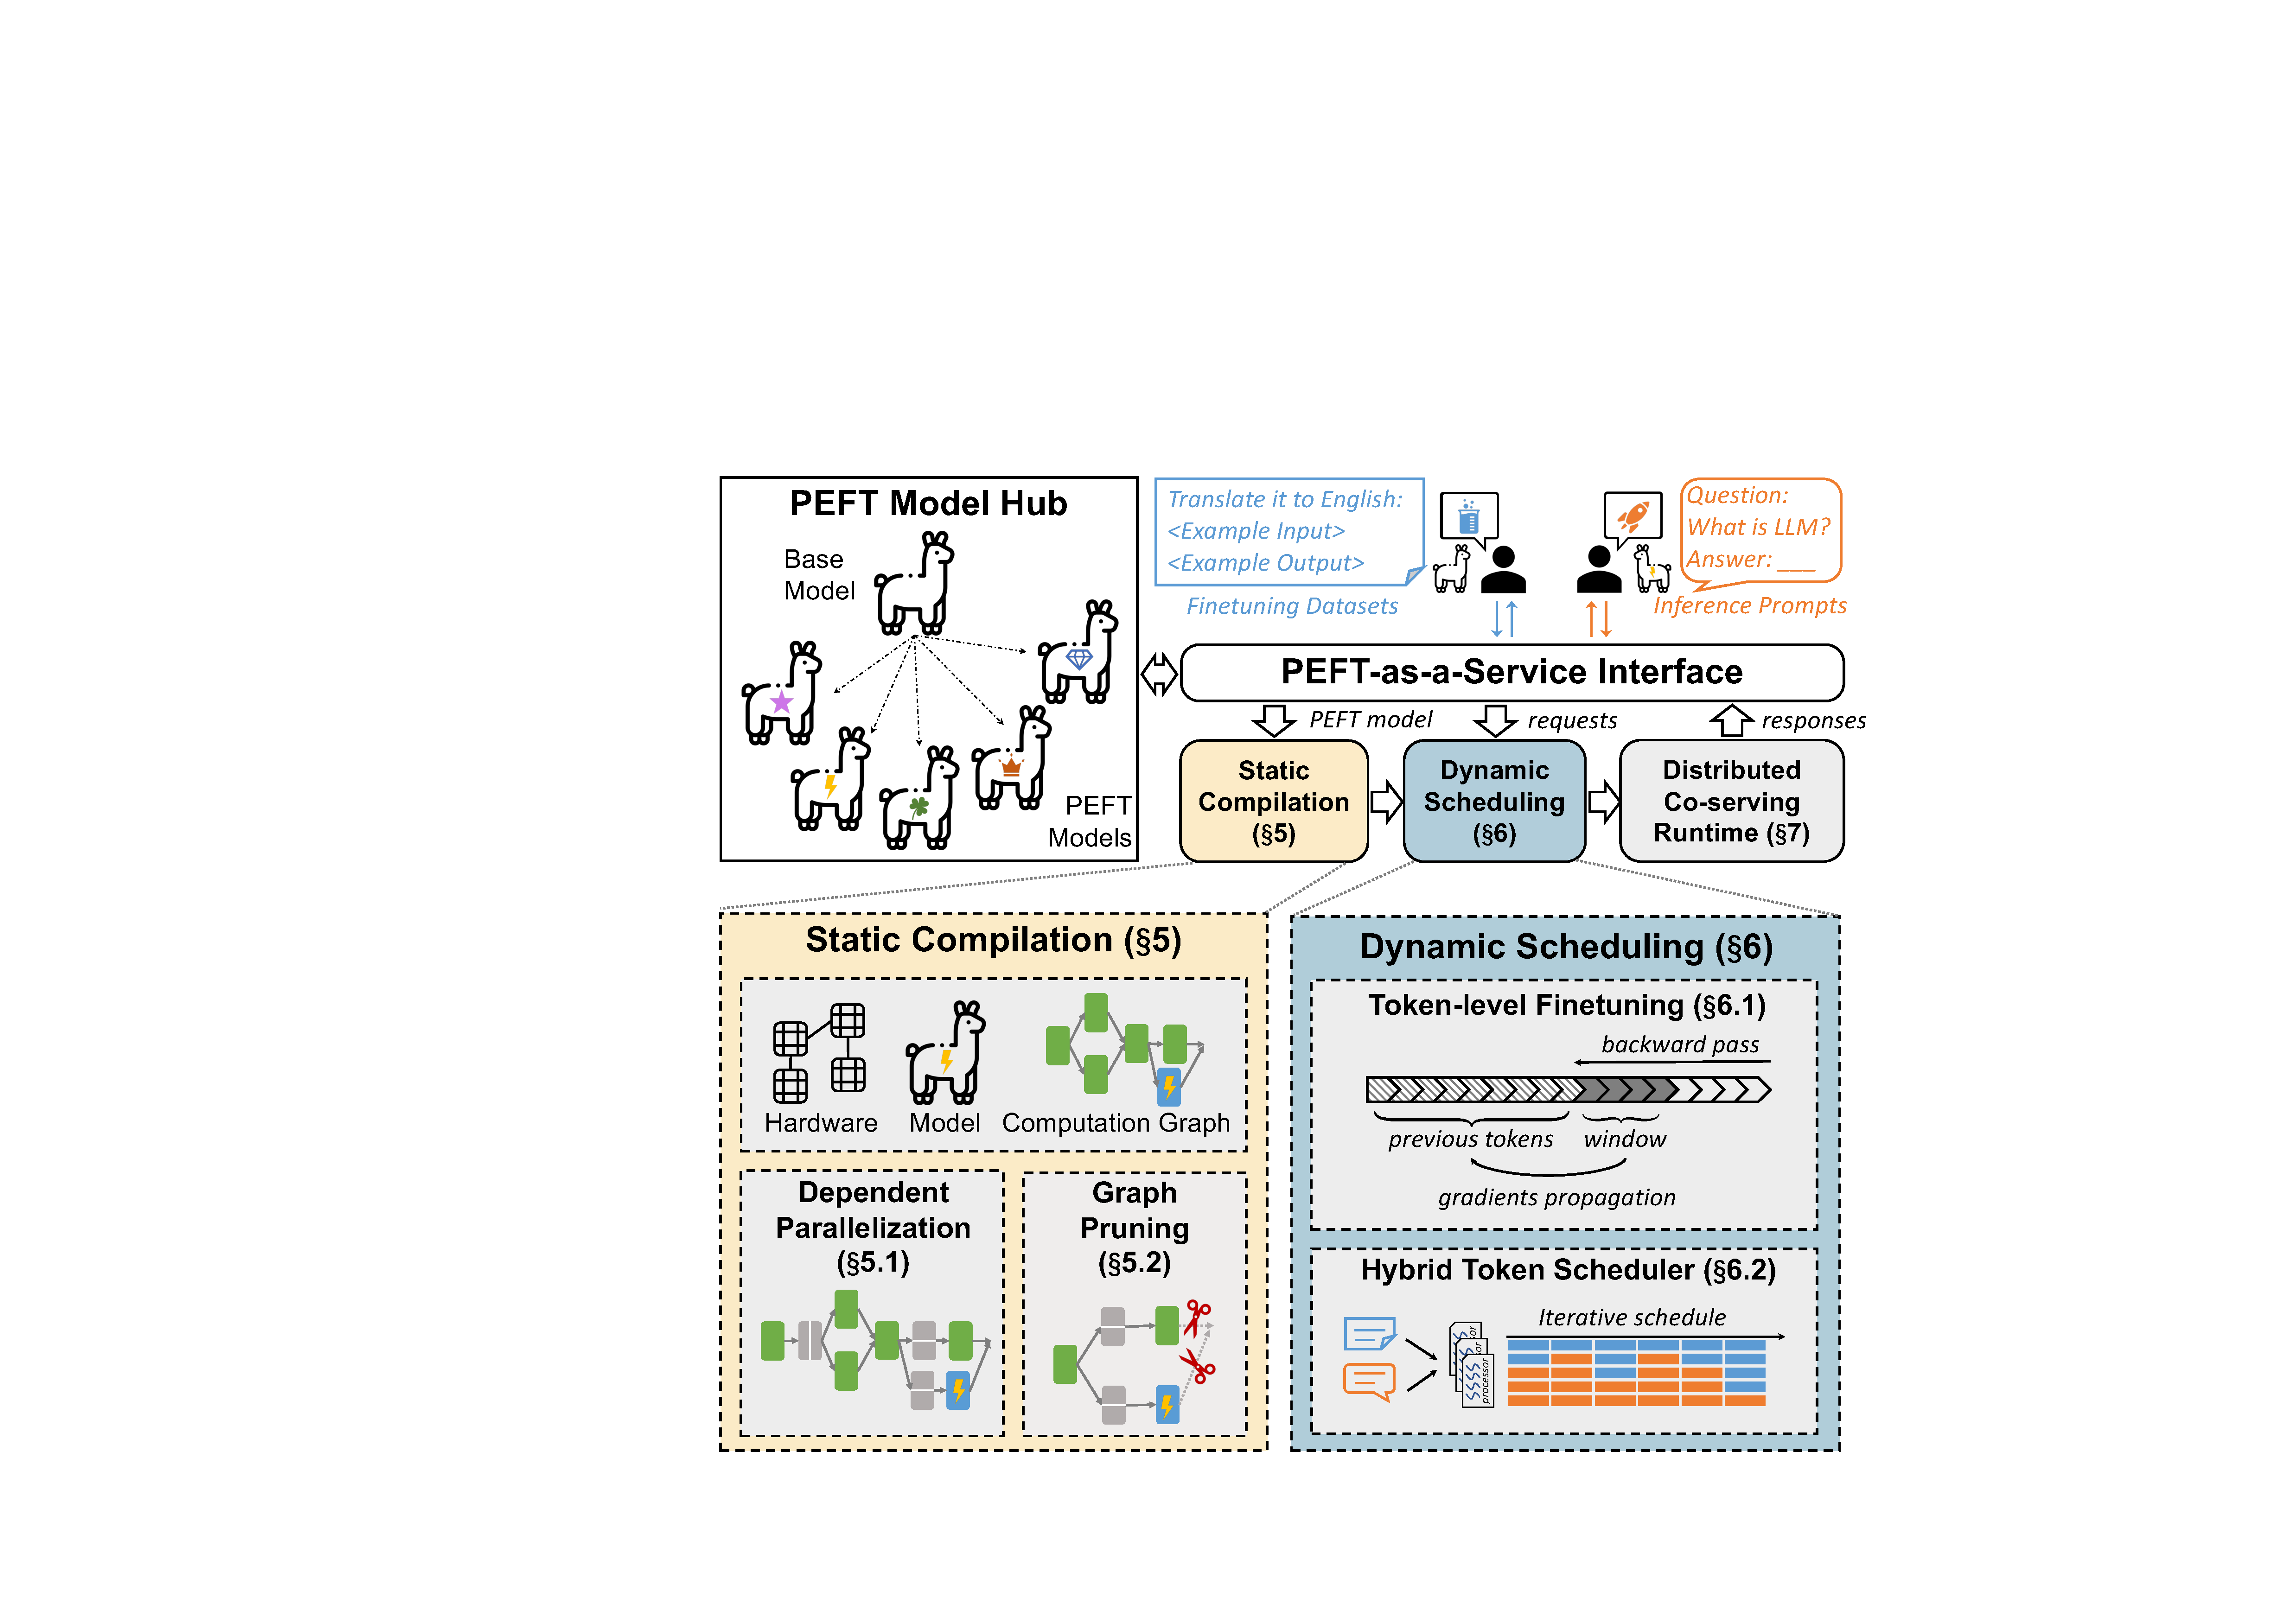
\includegraphics[width=0.8\linewidth]{figures/flexllm/overview4.pdf}
    \caption{An overview of \FlexLLM.}
    \label{flexllm:fig:overview}
\end{figure}

\Cref{flexllm:fig:overview} shows an overview of \FlexLLM, which co-serves both PEFT and inference requests for LLMs. Users can choose to use either finetuning or inference services on a model from the PEFT {\em model hub}, which stores the backbone LLM and all finetuned variants.
The programming interface for both inference and finetuning requests is unified through a \textit{PEFT-as-a-Service (PaaS) interface}.
\FlexLLM comprises three main components.
First, for finetuning requests that execute in parallel across multiple GPUs, the static compilation module (\Cref{flexllm:sec:compiler}) generates a parallel computation graph. This graph specifies the execution of the PEFT model over the distributed environment and optimizes the graph by pruning unnecessary tensors for memory saving.
Second, the dynamic scheduling module (\Cref{flexllm:sec:scheduling}) adopts a token-level finetuning mechanism. It mixes inference and finetuning tokens with a hybrid scheduling policy.
Finally, the computation graph and schedule plan are executed by \FlexLLM's distributed co-serving runtime (\Cref{flexllm:sec:impl}).

\begin{figure}[htbp]
    \centering
    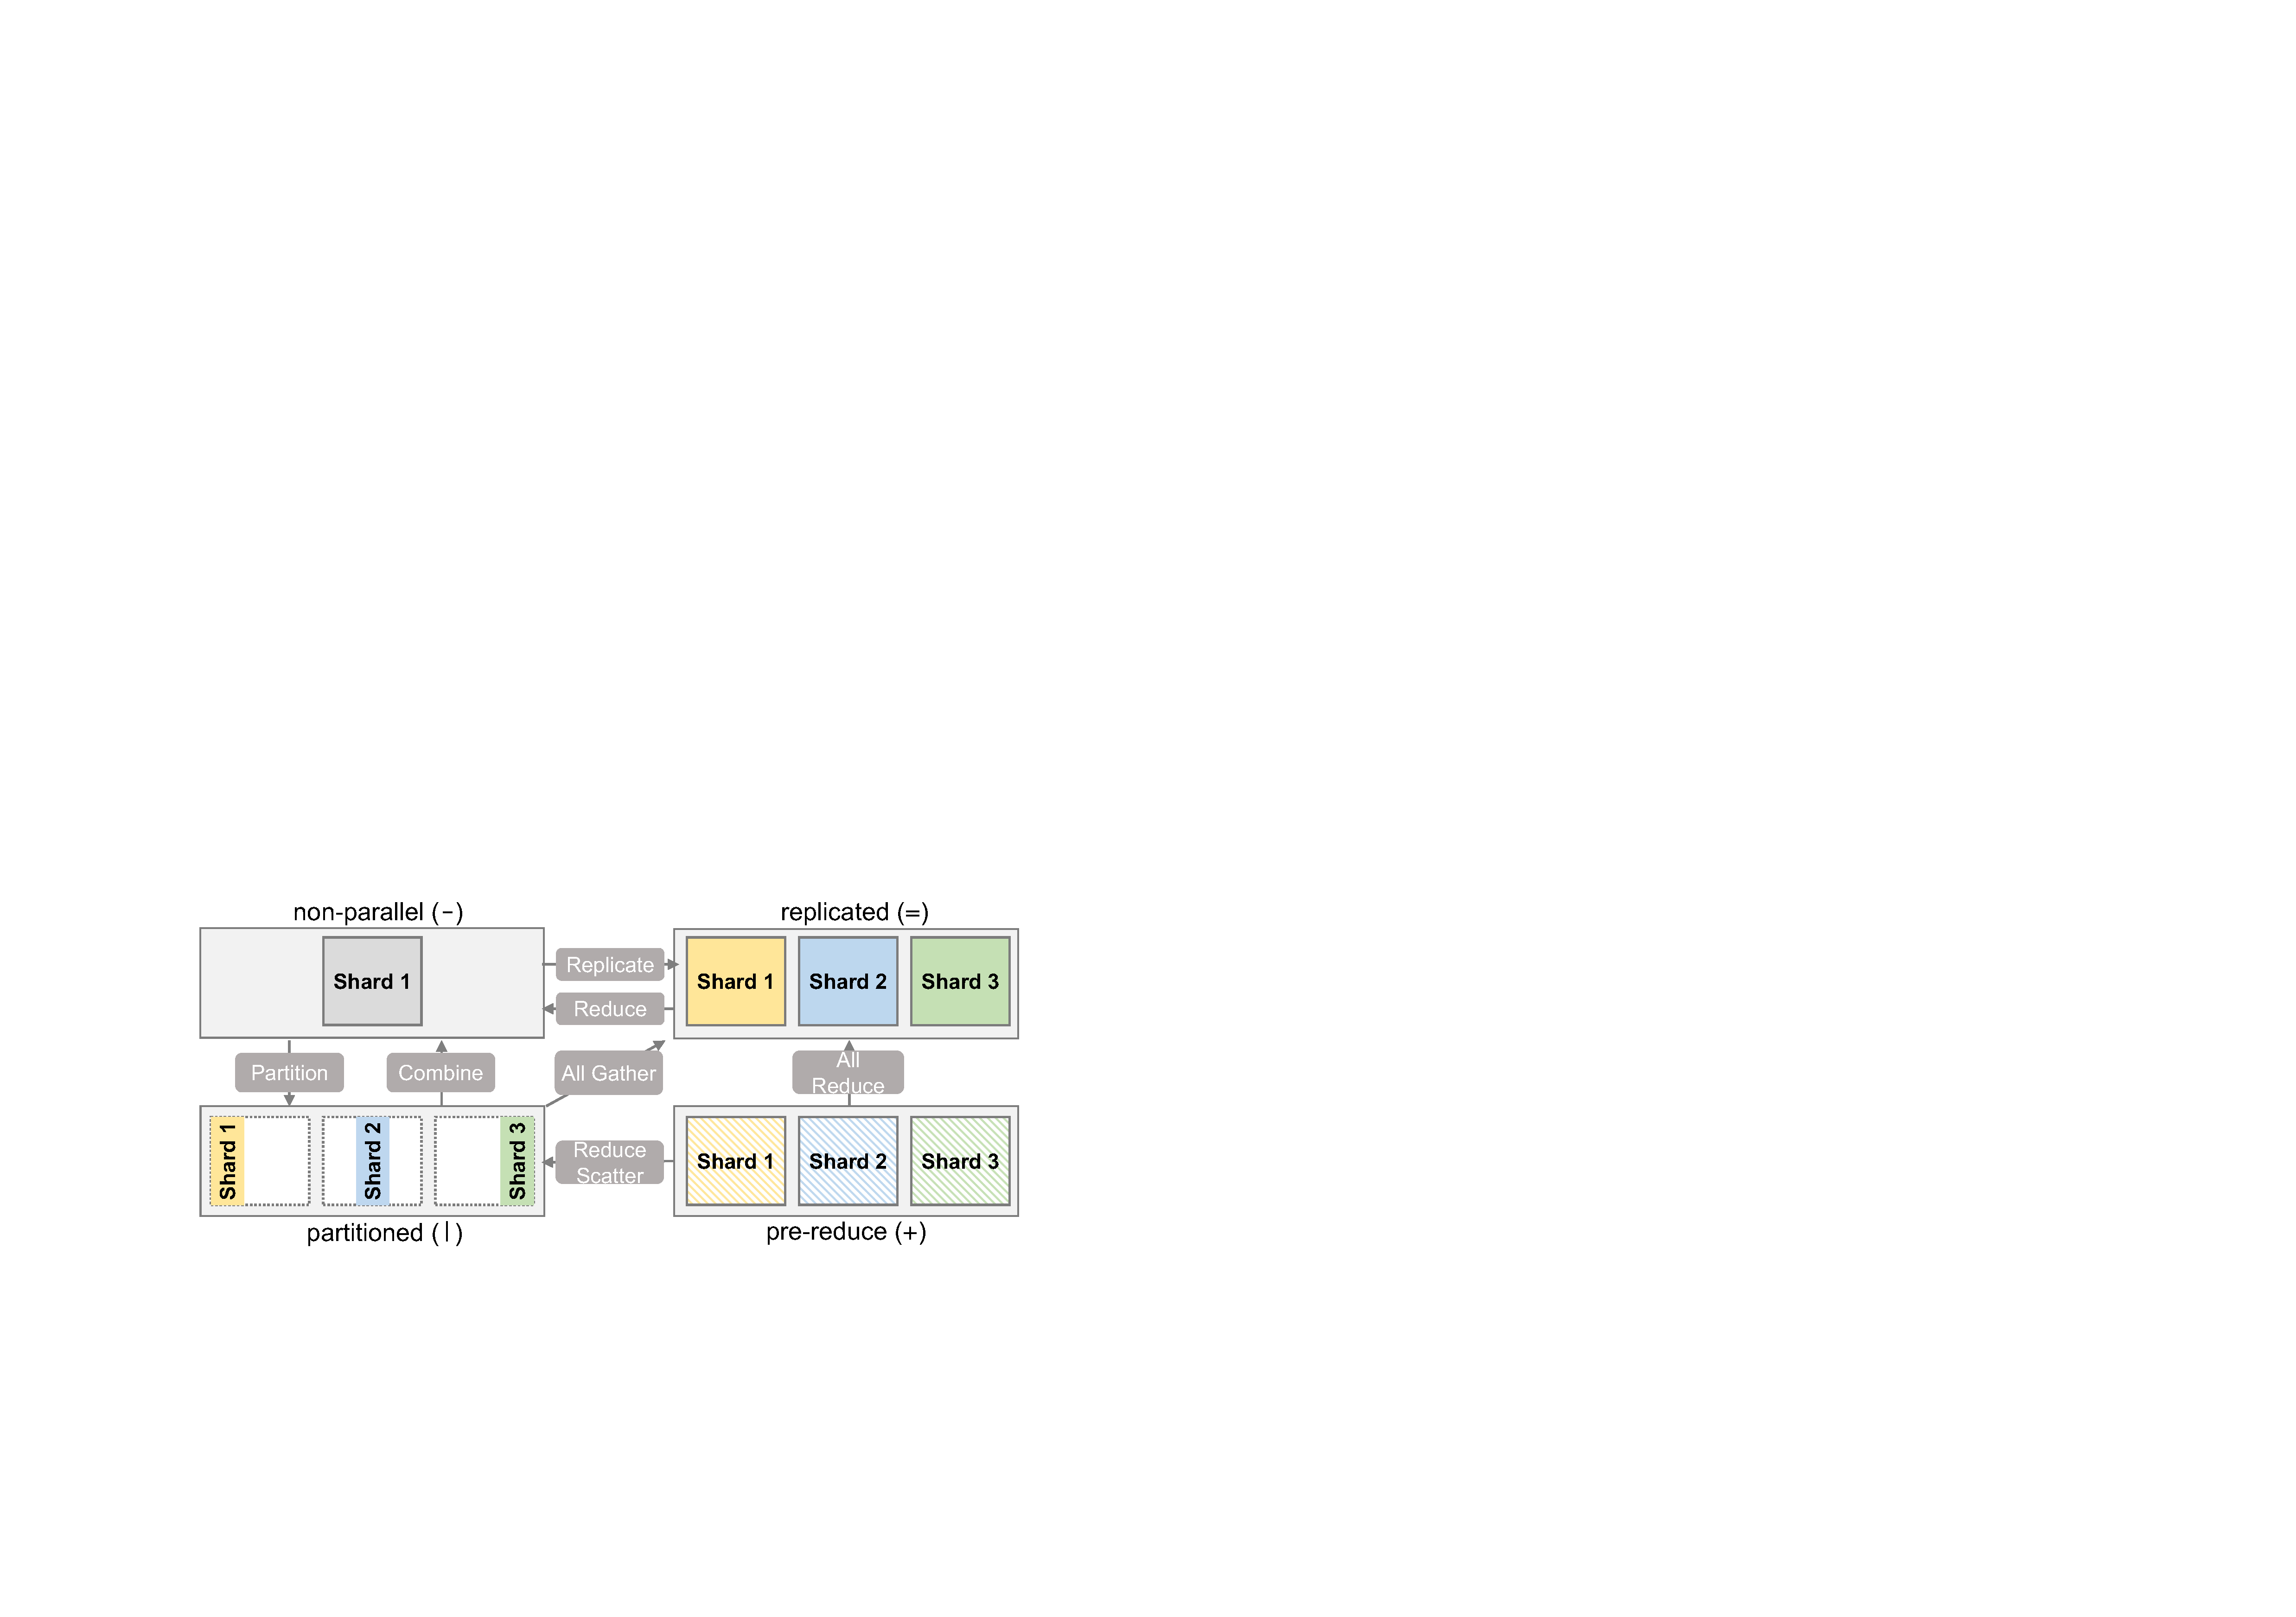
\includegraphics[width=0.7\linewidth]{figures/flexllm/pcg_states2.pdf}
    \caption{Four possible parallel states for a tensor dimension and their transitions. For each parallel state, the symbol in parentheses shows the notation \FlexLLM uses to represent it.}
    \label{flexllm:fig:pcg_states}
\end{figure}

\begin{figure}[htbp]
    \centering
    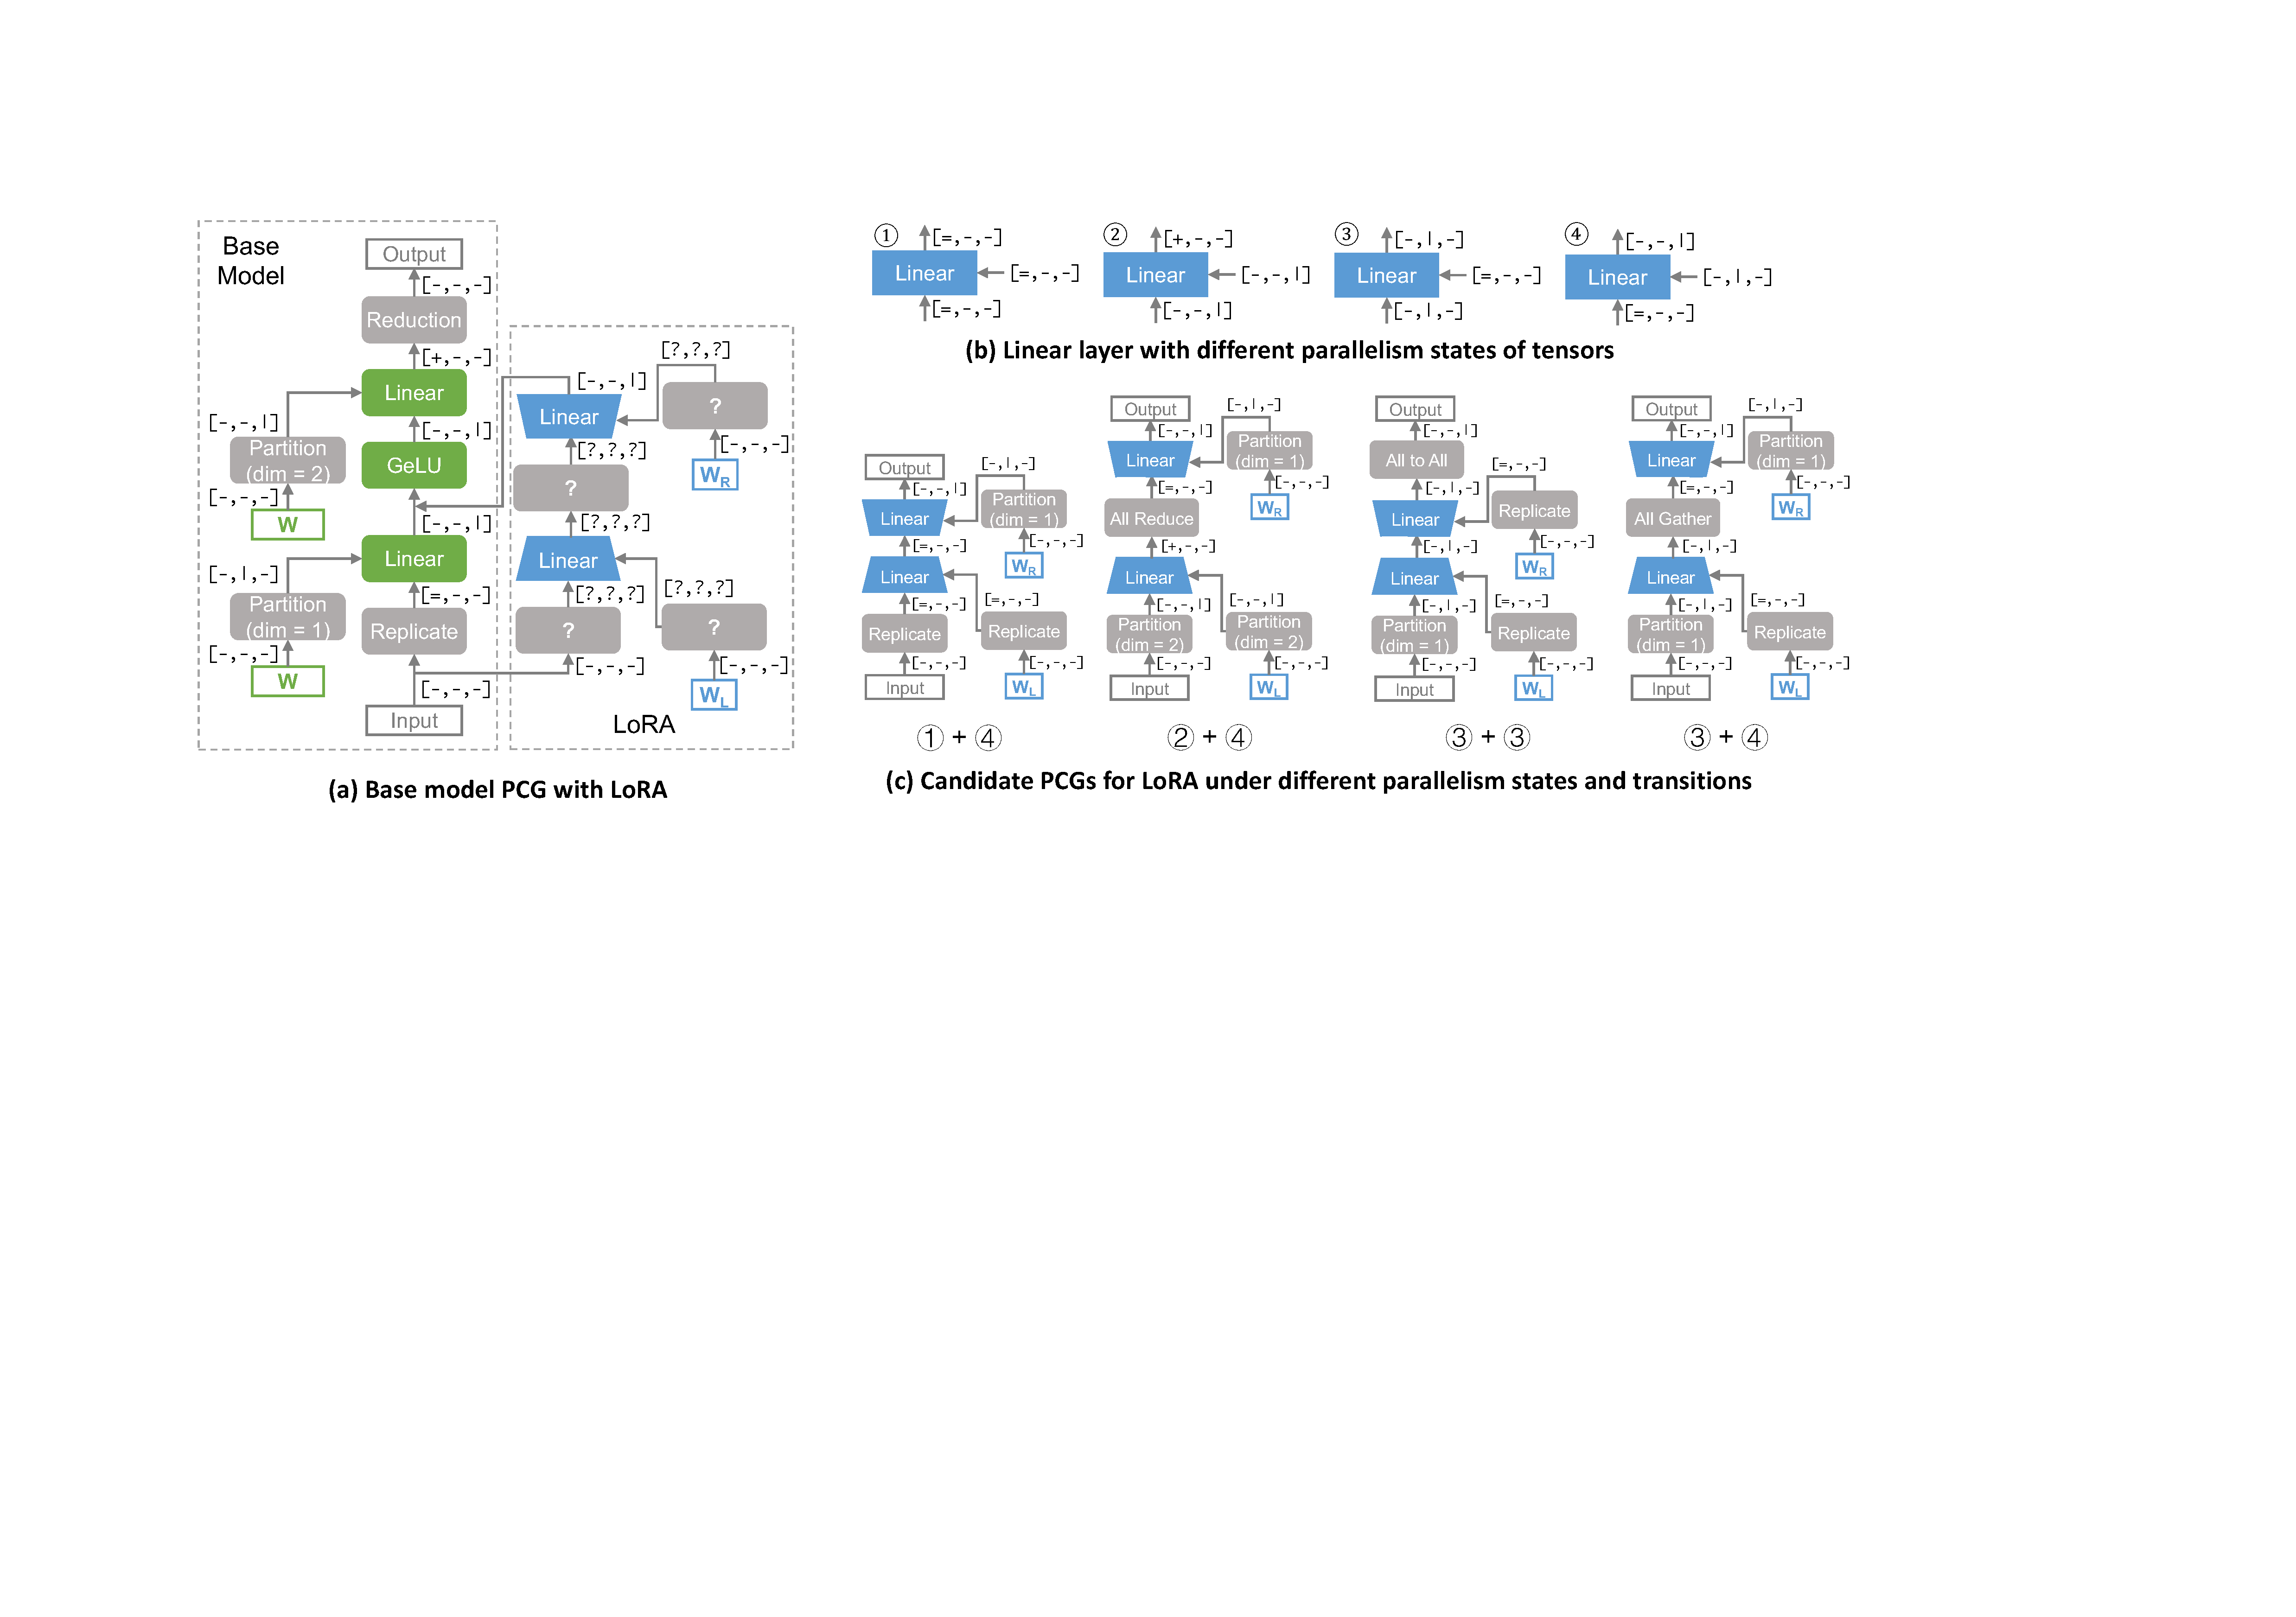
\includegraphics[width=\linewidth]{figures/flexllm/parallelization2.pdf}
    \caption{Illustration of \FlexLLM's different dependent parallelization strategies with the LoRA example. Each green (or gray) box indicates a compute (or parallelization) operator, and each edge between operators represents a parallel tensor, and the parallelization states of the tensor's dimensions are shown next to the edge.
    }
    \label{flexllm:fig:candidate_pcg}
\end{figure}

\subsection{PEFT-as-a-Service Interface}
\label{flexllm:subsec:paas_apis}

To facilitate the sharing of the backbone LLM across different tasks, \FlexLLM represents a PEFT model as a sequence of {\em bypass networks} attached to the backbone LLM.
%
Each bypass network takes a {\em single} tensor from the backbone LLM as input and produces a {\em single} output tensor, which is added to one tensor of the backbone LLM.
%
Let $X$ and $Y$ denote the input and output tensor of the bypass network, and let $f_B(X)$ and $f_A(X)$ denote the neural architecture of the backbone and bypass network for calculating $Y$. The bypass network can be formulated as $Y = f_B(X) + f_A(X)$.
%
All existing PEFT methods can be represented in this format. For instance, the (IA)$^3$ architecture modifies the topology of the backbone LLM by inserting an elementwise multiplication operator. It can be transformed into \FlexLLM's bypass network format since $Y = X\odot W = X + X \odot (W - O)$, where $\odot$ is elementwise multiplication and $O$ is a matrix of the same shape as $W$ whose elements are all one.
%
A significant benefit of this interface is that all PEFT models preserve the neural architecture of the backbone LLM, which enables \FlexLLM to fuse the computation graphs of different PEFT models.
%
\FlexLLM provides a unified user interface to launch inference and finetuning tasks by specifying a PEFT model and committing different types of input data, such as finetuning datasets or inference prompts.

\section{Static Compilation}
\label{flexllm:sec:compiler}

Once a PEFT model is registered, \FlexLLM compiles it into a parallel computation graph (PCG)~\cite{unger2022unity}. To optimize finetuning performance, \FlexLLM applies two key static compilation optimizations to discover an optimized PCG: {\em dependent parallelization} (\Cref{flexllm:subsec:parallelization}) and {\em graph pruning} (\Cref{flexllm:subsec:pruning}).

\subsection{Dependent Parallelization}
\label{flexllm:subsec:parallelization}

To minimize memory overhead, \FlexLLM allows finetuning and inference tasks to utilize the same backbone LLM and share memory allocated for both model weights and intermediate activations. This approach avoids redundant memory consumption while requiring the parallelization strategies of the PEFT models to be compatible with that of the backbone LLM, a task termed {\em dependent parallelization}.

Existing auto-parallelization approaches like Alpa~\cite{zheng22-alpa} and Unity~\cite{unger2022unity} can identify optimal parallelization strategies for backbone LLMs.
\FlexLLM extends the optimization target to also include the bypass networks in PEFT models.
To achieve this goal, \FlexLLM generalizes the {\em parallel computation graph} (PCG) abstraction introduced in Unity~\cite{unger2022unity} by associating a {\em state} field with each tensor dimension.

\Cref{flexllm:fig:pcg_states} shows the four possible tensor states when parallelizing a tensor, including {\em non-parallel} ({\tt -}), {\em partitioned} ({\tt |}), {\em replicated} ({\tt =}), and {\em pre-reduce} ({\tt +}), as well as the state transitions.
Given the fixed parallelization of the backbone LLM, \FlexLLM searches for an optimal PCG for each bypass network by enumerating possible parallelization operators---{\tt partition}, {\tt combine}, {\tt replicate}, and {\tt reduce}---inferring output tensor states, and validating their compatibility.
\Cref{flexllm:fig:candidate_pcg} shows four candidate PCGs discovered by \FlexLLM for parallelizing a LoRA network. To select the best strategy, \FlexLLM reuses Unity's profiling-based cost model~\cite{unger2022unity} and chooses the candidate PCG with the lowest estimated execution cost.

\begin{algorithm}[htbp]
\caption{Static graph pruning. For an operator $n$, $\textproc{UpdateInput}(n, \mathcal{O}(n))$ returns a set of input tensors needed in order only to compute $\mathcal{O}(n)$ of the operator.}
\label{flexllm:alg:graph_pruning}
\begin{algorithmic}[1]
\State {\bf Inputs:} PCG of a PEFT model $\mathcal{G}$
\State {\bf Outputs:} $\mathcal{A}$ is a set of tensors to be memorized, $\mathcal{R}$ is a set of tensors to be rematerialized
\flexllmLeftComment{Step 1: computation graph pruning}
\State $\overline{\mathcal{G}} = \Call{ReverseAutoDiff}{\mathcal{G}}$
\State $\mathcal{Q} = \emptyset$ \Comment{$\mathcal{Q}$ is a queue of updated operators}
\For{operator $n \in \overline{\mathcal{G}}$}
\For{output tensor $t \in \mathcal{O}(n)$}
\If{$t$ is the weight gradient of the base LLM}
\State $\mathcal{O}(n) = \mathcal{O}(n) \setminus \{t\}$
\State $\mathcal{I}(n) = \Call{UpdateInput}{n, \mathcal{O}(n)}$
\State $\mathcal{Q}$.push\_back($n$)
\EndIf
\EndFor
\EndFor
\While{$\mathcal{Q}$ is not empty}
\State $n = \mathcal{Q}$.pop\_front()
\For{output tensor $t \in \mathcal{O}(n)$}
\If{$\nexists u. t \in \mathcal{I}(u)$ }
\State $\mathcal{O}(n) = \mathcal{O}(n) \setminus \{t\}$
\State $\mathcal{I}(n) = \Call{UpdateInput}{n, \mathcal{O}(n)}$
\State $\mathcal{Q}$.push\_back($n$)
\EndIf
\EndFor
\EndWhile
\State $\mathcal{A} = \emptyset$
\For{operator $n \in \mathcal{G}$}
\For{tensor $t \in \mathcal{O}(n)$}
\If{$\exists u \in \overline{\mathcal{G}}. t \in \mathcal{I}(u)$}
\State $\mathcal{A} = \mathcal{A} \cup \{ t\}$
\EndIf
\EndFor
\EndFor
\flexllmLeftComment{Step 2: opportunistically rematerializing tensors}
\For{tensor $t \in \mathcal{A}$}
\State Let $n$ be the operator that outputs $t$ (i.e., $t \in \mathcal{O}(n)$)
\If{$\mathcal{I}(n) \subseteq \mathcal{A}$ and $\Call{Cost}{n} < threshold$}
\State $\mathcal{A} = \mathcal{A} \setminus \{t\}$, $\mathcal{R} = \mathcal{R} \cup \{t\}$
\EndIf
\EndFor
\State {\bf return} $\mathcal{A}, \mathcal{R}$
\end{algorithmic}
\end{algorithm}

\begin{figure}[htbp]
    \centering
    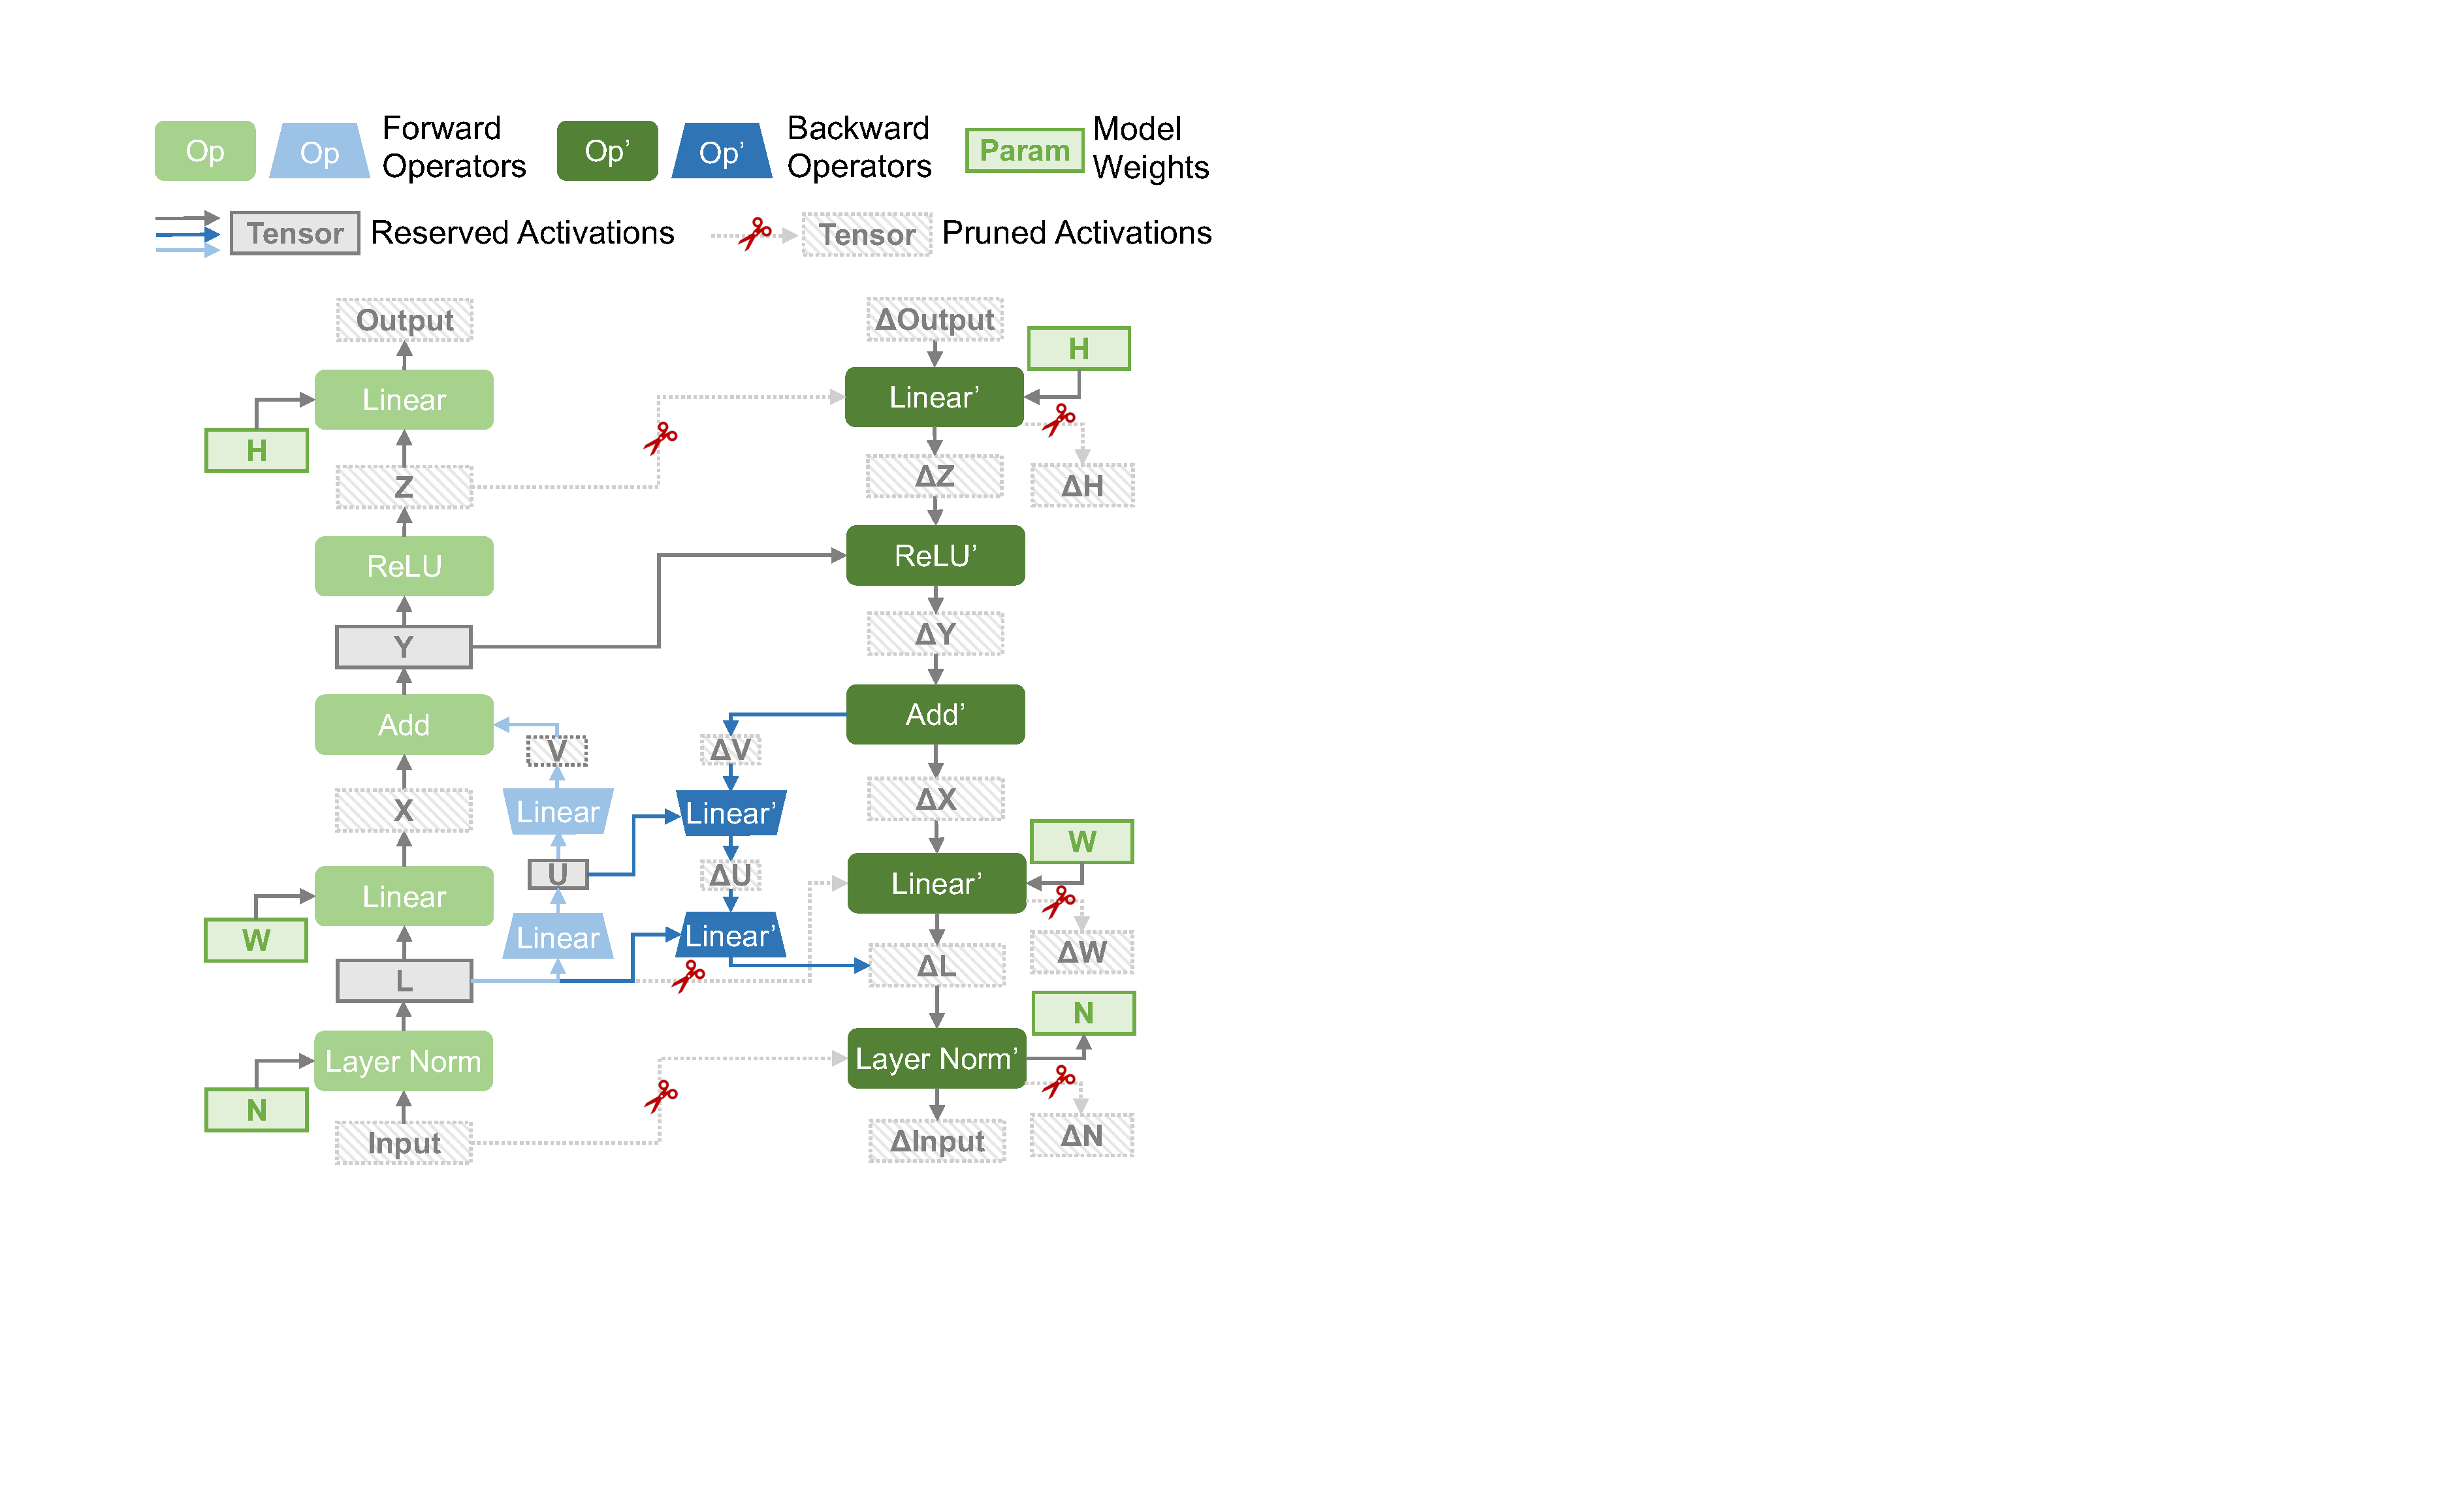
\includegraphics[width=0.65\linewidth]{figures/flexllm/graph_pruning2.pdf}
    \caption{Static graph pruning for an MLP model with LoRA.}
    \label{flexllm:fig:graph_pruning}
\end{figure}

\begin{figure}[htbp]
    \centering
    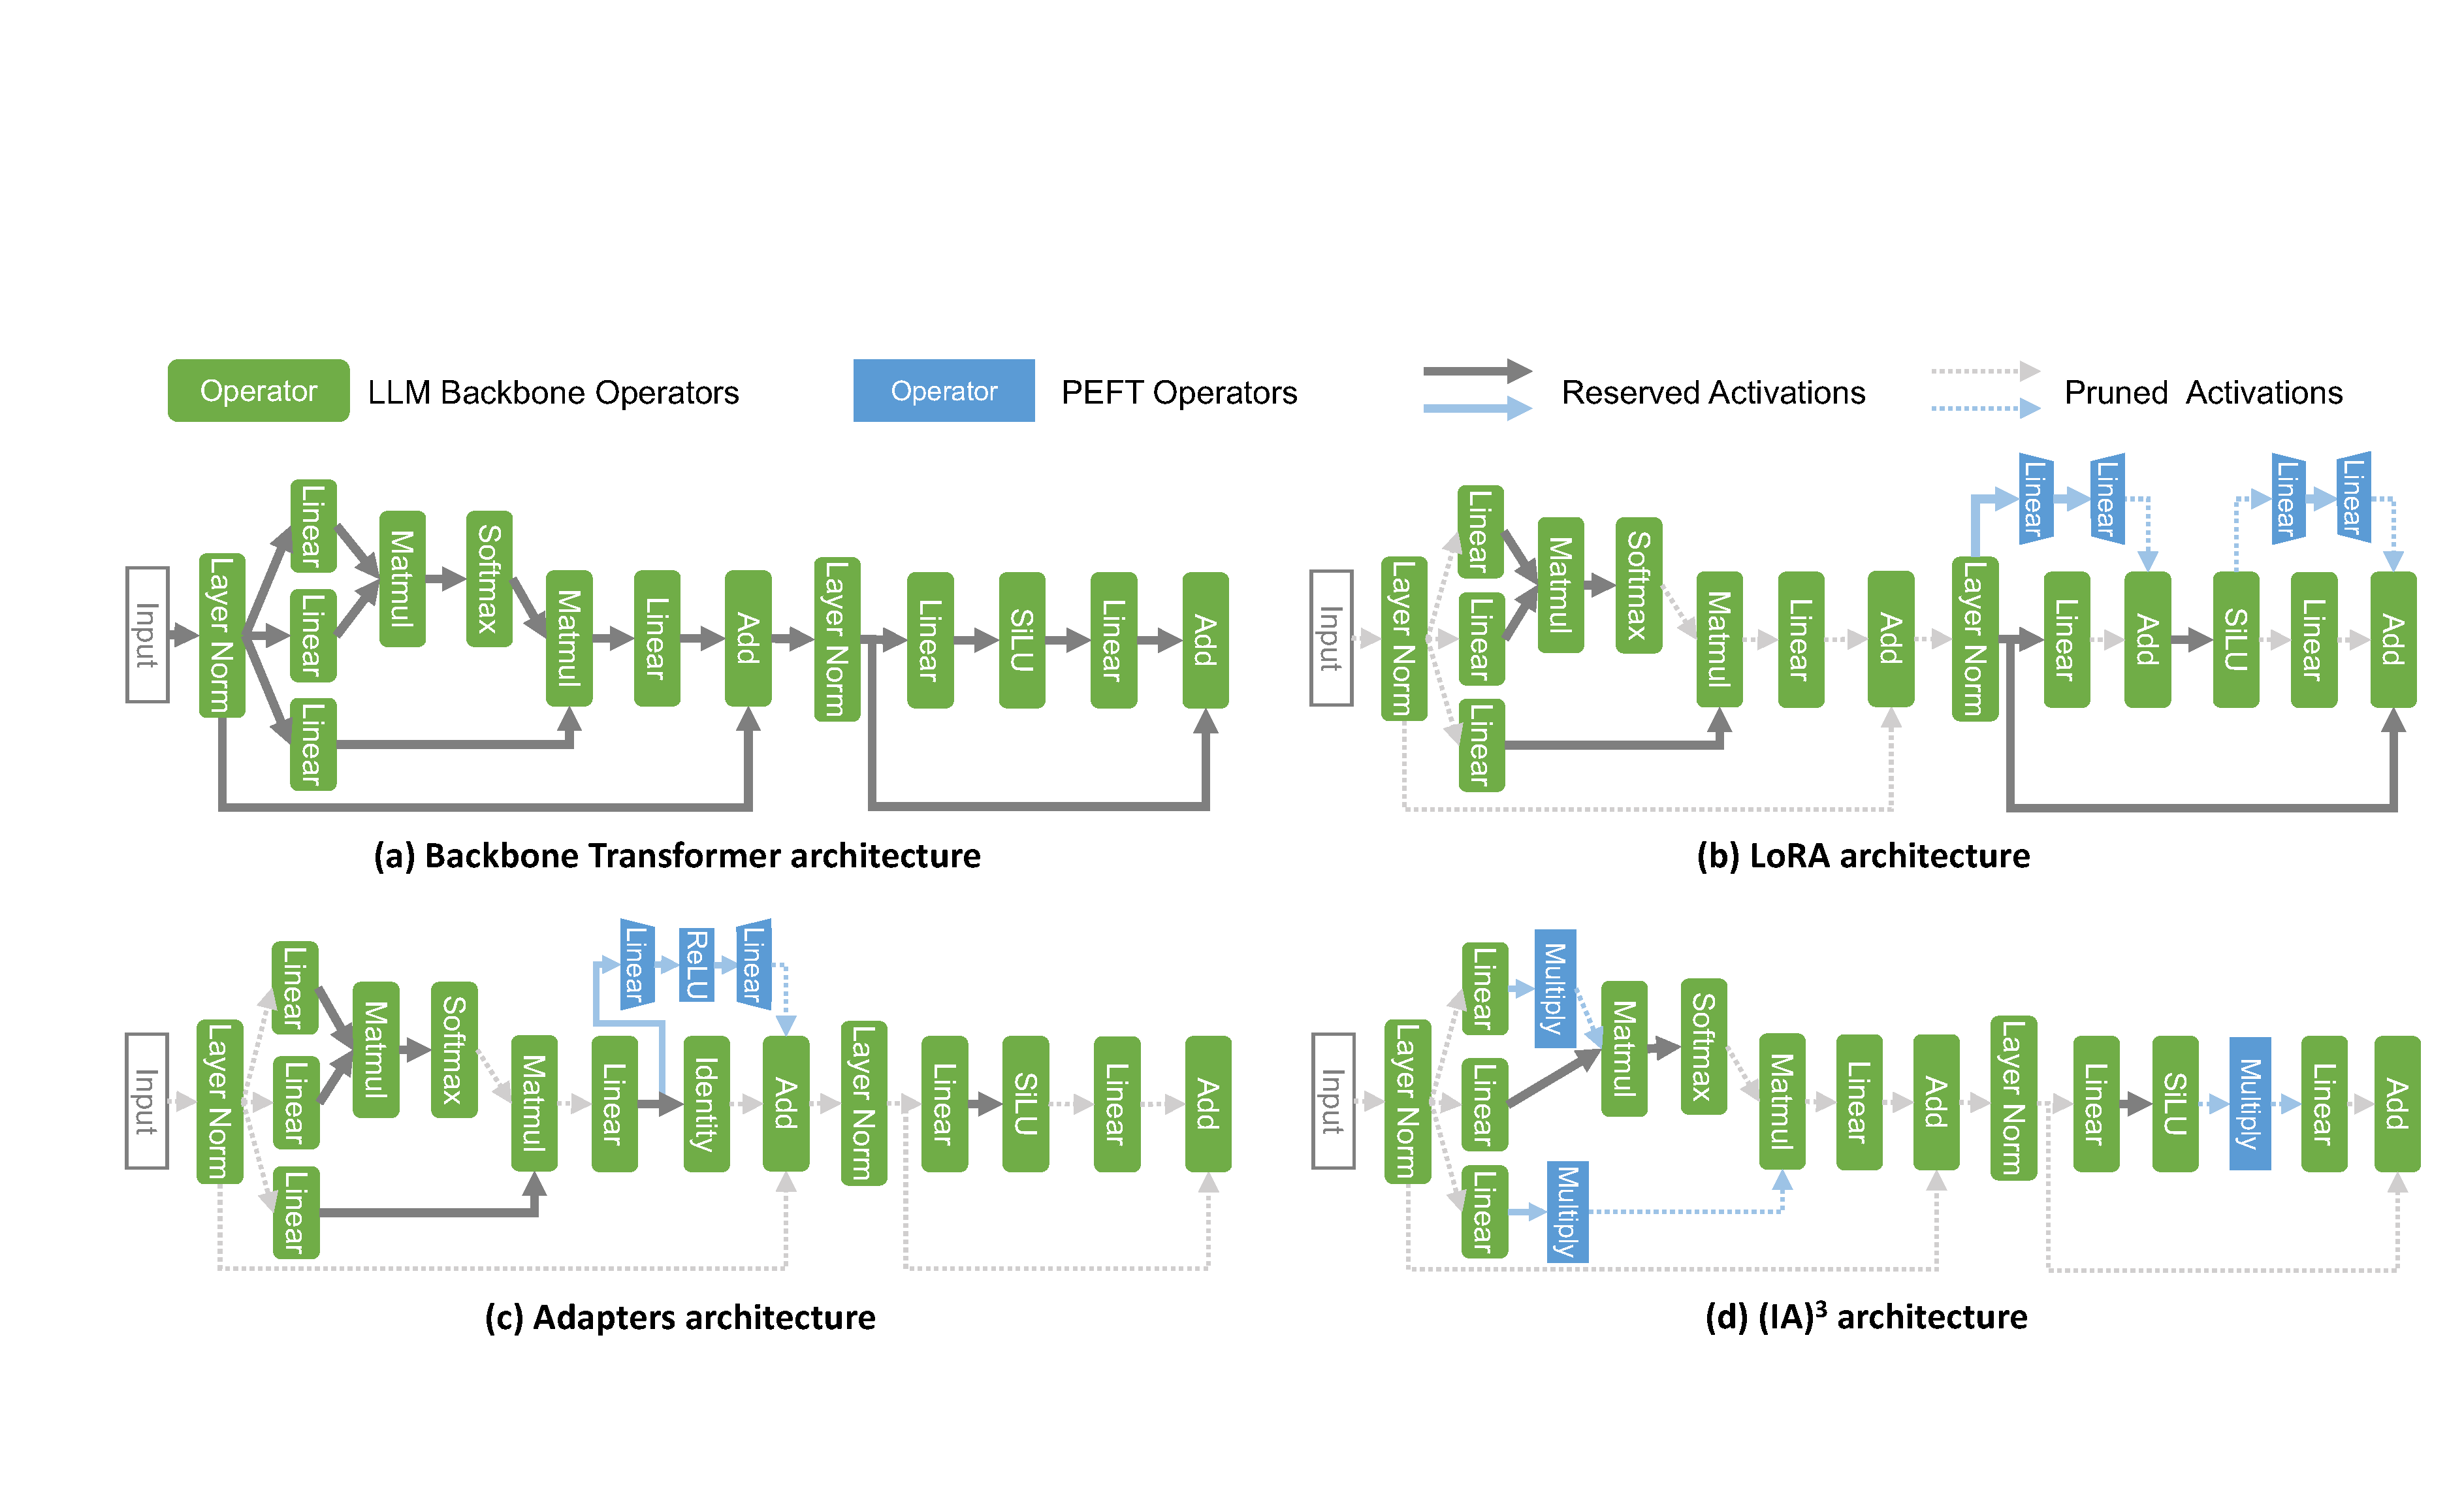
\includegraphics[width=0.9\linewidth]{figures/flexllm/architecture2.pdf}
    \caption{An overview of existing parameter-efficient finetuning (PEFT) methods. Green boxes show the operators of the backbone LLM, while blue boxes are the operators introduced by different PEFT methods. Arrows represent intermediate activations to be reserved and the dashed arrows demonstrate they are pruned by \FlexLLM.}
    \label{flexllm:fig:peft-methods}
\end{figure}

\subsection{Graph Pruning}
\label{flexllm:subsec:pruning}

\FlexLLM's {\em graph pruning} algorithm takes as input a PEFT model and its backbone LLM, and outputs a minimal set of intermediate activations that must be reserved to perform finetuning of the bypass networks.
%
This pruning process requires reasoning over data dependencies between operators, specifically their input and output tensors. Importantly, this pruning process preserves model quality since gradients with respect to frozen parameters are mathematically unnecessary for PEFT optimization and do not affect the final trained model. To facilitate the analysis of data dependencies, \FlexLLM introduces additional notation in the PCG representation.
Let $\mathcal{G}=(\mathcal{N}, \mathcal{E})$ denote the PCG of a PEFT model, where each node $n \in \mathcal{N}$ represents a tensor algebra (or parallelization) operator, and each edge $e=(n_1, n_2) \in \mathcal{E}$ is a tensor shared between operators. For a node $n$, let $\mathcal{I}(n)$ and $\mathcal{O}(n)$ denote its set of input and output tensors.
%
By definition, $(n_1, n_2) \in \mathcal{E}$ if and only if $\mathcal{O}(n_1) \cap \mathcal{I}(n_2) \neq \emptyset$, i.e., when at least one output tensor of $n_1$ serves as an input to $n_2$.

The design of \FlexLLM's graph pruning algorithm is based on two key observations.
%
First, conventional ML training procedures maintain all intermediate activations during the forward pass to compute gradients in the backward pass.
%
However, due to the linear algebra nature of most operators, these intermediate activations are primarily used to compute gradients with respect to the base LLM's trainable parameters. In the case of PEFT, the backbone LLM parameters are frozen, and only the parameters in the bypass networks are updated.
%
This insight allows \FlexLLM to eliminate most intermediate activations, retaining only those necessary for computing gradients of the bypass networks.
Second, different PEFT methods connect bypass networks at varying locations within the backbone LLMs, and therefore require different subsets of intermediate activations for backpropagation.
\Cref{flexllm:fig:peft-methods} illustrates examples of how various PEFT methods attach their bypass networks to the base LLM.

Building on these observations, \FlexLLM performs {\em static} graph pruning during the construction of the PCG for each registered PEFT model, and {\em dynamic} scheduling to manage finetuning and inference tasks, along with corresponding memory allocations (see \Cref{flexllm:sec:scheduling}).
%
\Cref{flexllm:alg:graph_pruning} shows \FlexLLM's graph pruning algorithm, with \Cref{flexllm:fig:graph_pruning} illustrating the process for an MLP model with LoRA. Given a PEFT model's PCG $\mathcal{G}$, the algorithm generates an execution plan specifying which intermediate activations to cache for efficient backpropagation.

The algorithm constructs the backward graph $\overline{\mathcal{G}}$ using reverse-mode automatic differentiation~\cite{hogan2014fast}, then prunes gradients for frozen base LLM weights. It iteratively processes operators to discover pruning opportunities, ultimately identifying the minimal set of activations $\mathcal{A}$ required for the backward pass. \FlexLLM combines this with {\em rematerialization} and {\em activation compression}.

\paragraph{Rematerialization and compression.}
\FlexLLM applies tensor rematerialization~\cite{checkmate}, selectively discarding tensors in the forward pass and recomputing them during backpropagation. For each tensor $t \in \mathcal{A}$ after graph pruning, \FlexLLM rematerializes $t$ if all input tensors are stored and recomputation has low overhead. Additionally, \FlexLLM opportunistically applies lossless compression when operators like {\tt ReLU} don't require access to original input tensors.
Consider $y=\texttt{ReLU}(x) = \max{(x, 0)}$, whose derivative is $\partial y/\partial x = 1$ for $x>0$ and $0$ for $x\leq0$. Therefore, instead of storing the original input tensor $x$, \FlexLLM keeps the bitmask of $x$.

\section{Dynamic Scheduling}
\label{flexllm:sec:scheduling}
Once static compilation produces an executable generalized PCG for a PEFT model, \FlexLLM must determine an execution schedule capable of concurrently handling both finetuning and inference requests.
%
This is particularly challenging due to the distinct characteristics of these two workloads.
%
First, inference requests arrive in an online and highly dynamic manner, requiring the system to rapidly adapt GPU resource allocation to maintain low-latency responses. In contrast, finetuning involves both a forward pass---similar to inference---and a backward pass to update model parameters.
Additionally, auto-regressive inference for generative LLMs proceeds in a token-by-token fashion, while finetuning is typically performed at the sequence level to maximize throughput.
To address these challenges, \FlexLLM introduces a novel \textit{token-level finetuning} mechanism along with a \textit{hybrid token scheduler}.

\begin{figure}[htbp]
    \centering
    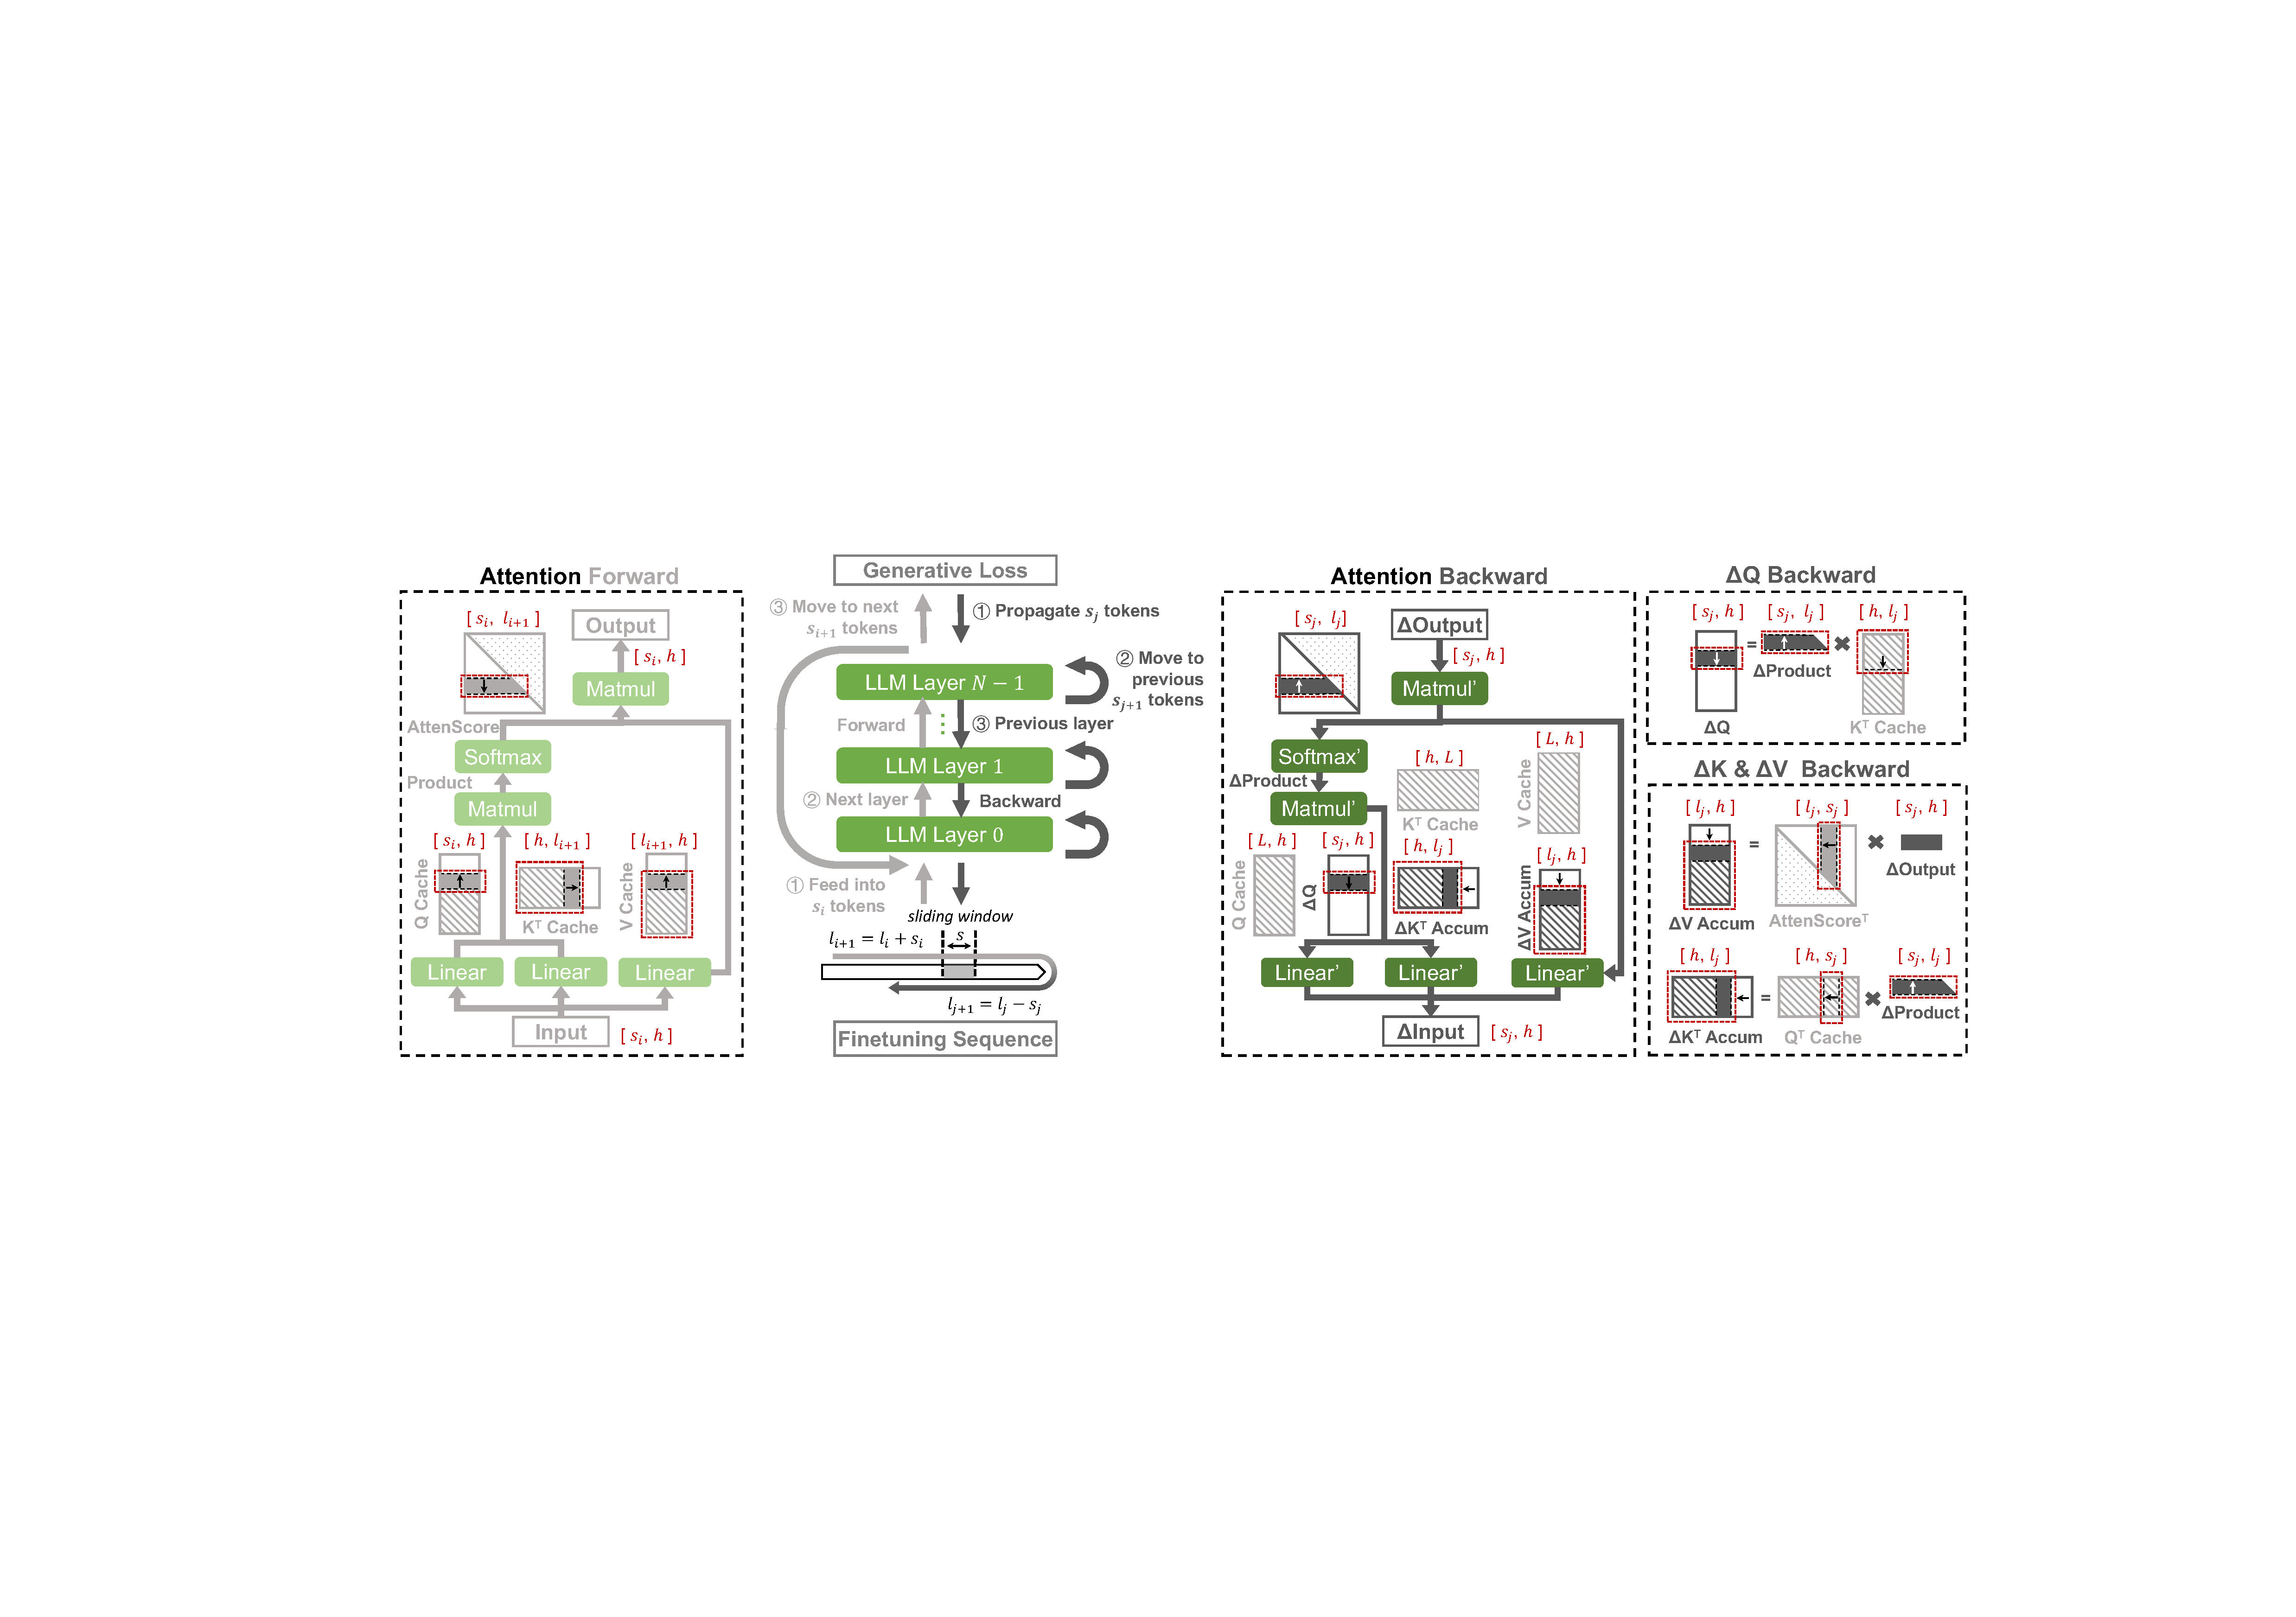
\includegraphics[width=\linewidth]{figures/flexllm/tokenlevel2.pdf}
    \caption{Illustration of the attention module's forward and backward execution with \FlexLLM's token-level finetuning mechanism.}
    \label{flexllm:fig:token-level-finetuning}
\end{figure}

\begin{figure}[htbp]
    \centering
    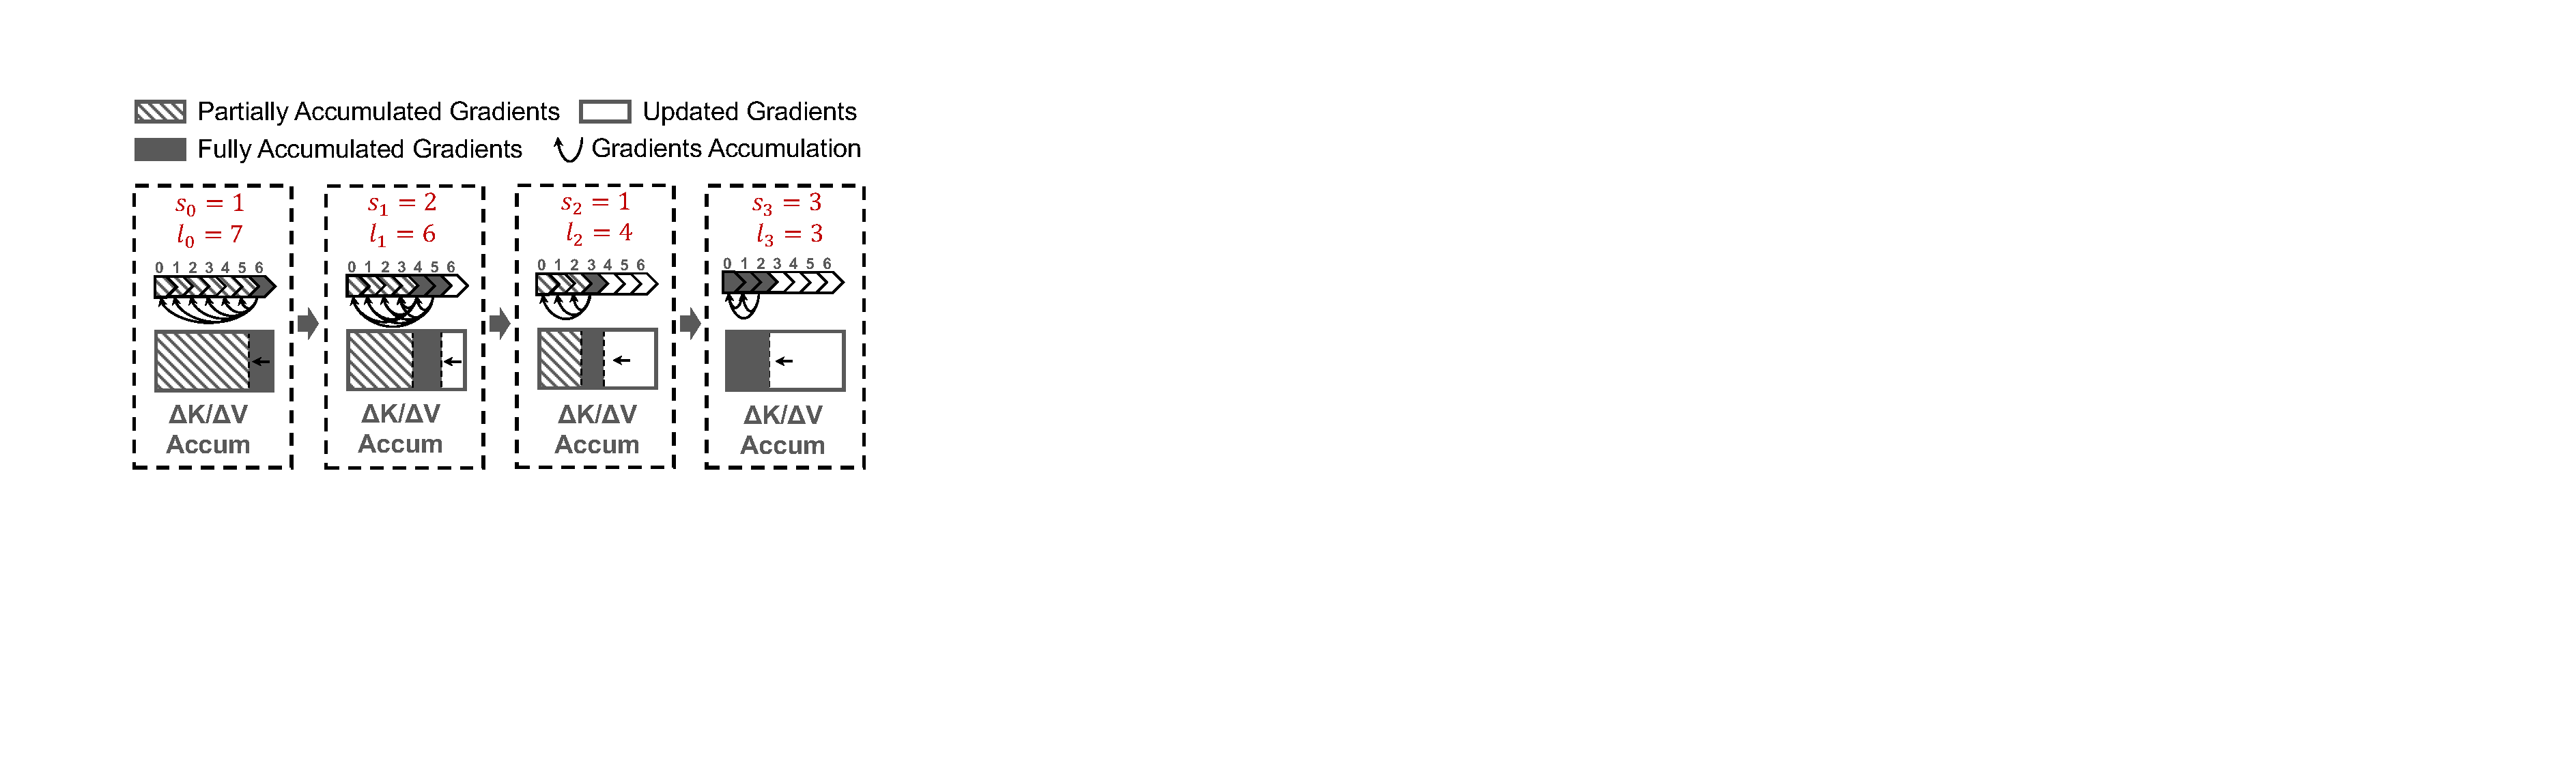
\includegraphics[width=0.6\linewidth]{figures/flexllm/blockwise_back2.pdf}
    \caption{Illustration of KV gradients accumulation in the backward pass of \FlexLLM's token-level finetuning mechanism, where $s_j$ and $l_j$ are the window length and the starting position of the $j$-th slice of the sequence.}
    \label{flexllm:fig:token-level-backword}
\end{figure}

\subsection{Token-Level Finetuning}
\label{flexllm:subsec:incremental_finetuning}

Processing a finetuning request typically involves performing both forward and backward passes across all model layers for the entire input sequence.
When co-served with inference requests, this sequence-level execution can significantly interfere with the token-wise inference kernels and degrade system goodput---that is, the effective inference throughput that meets latency SLOs.

While sequence-level parallelism~\cite{megatron-sp,deepspeed-ulysses} could help reduce the added finetuning latency per GPU, this approach would suffer from coarse-grained scheduling, forcing the system to wait for entire finetuning sequences to complete before reallocating resources to handle inference bursts.

To address this problem and maximize GPU utilization, \FlexLLM introduces a \textit{token-level finetuning} mechanism, detailed in \Cref{flexllm:alg:token-level-finetuning}. The key idea is to decompose the finetuning computation into smaller steps using a dynamic sliding window over tokens. This window spans both the forward and backward passes, with its size dynamically determined by the hybrid token scheduler (lines 4 and 15) to ensure that inference requests continue to meet their SLO constraints (\Cref{flexllm:subsec:scheduler}).

During the forward pass (lines 3--11), the finetuning sequence is partitioned into windows of $s_i$ tokens (line 5), which are incrementally fed into the model. The model processes each token window layer by layer (lines 7--8), computes the generative loss for the window (line 10), and then advances to the next set of tokens (line 11).
To preserve the semantics of full sequence-level finetuning, \FlexLLM caches key and value tensors---similar to incremental decoding in inference~\cite{yu2022orca}---as well as query tensors, which are reused during backward attention computations. This caching follows the {\em causal mask} constraint inherent in LLMs.

During the backward pass (lines 12--21), \FlexLLM executes the model layers in reverse order (line 13).
Within each layer, the finetuning request is again divided into token windows (lines 14--16).
However, unlike the relatively straightforward forward pass, token-level backward execution of the attention module is more complex due to auto-regressive token dependencies.

\Cref{flexllm:fig:token-level-finetuning} illustrates the forward and backward PCGs of the attention module. When computing gradients for $s_j$ tokens, the resulting gradients $\Delta Q$, $\Delta K$, $\Delta V$ have shapes $[s_j, h]$ for queries but $[l_j, h]$ for keys and values due to autoregressive attention dependencies (\Cref{flexllm:fig:token-level-backword}). \FlexLLM accumulates KV gradients across steps, applying them only after complete backward traversal. This accumulation strategy minimally increases memory consumption due to layer-wise execution enabling workspace memory reuse.

\begin{algorithm}[htbp]
\caption{Token-level finetuning mechanism.}
\label{flexllm:alg:token-level-finetuning}
\begin{algorithmic}[1]
\State {\bf Inputs}: PEFT model $M$ of depth $N$; finetuning request $r$ with sequence length $L$
\State {\bf Outputs}: PEFT model gradients $\Delta M$
\For{$i\gets 0, l_0 \gets 0$; $l_i<L$; $i\texttt{++}$} \Comment{Forward pass}
\State $s_i\gets \Call{HybridTokenScheduler}{l_i, L}$
\State $r_i \gets \Call{Slice}{r, l_i, s_i}$
\State $X_{0,i} \gets \Call{Tokenize}{r_i}$
\For{model layer index $n \in \Call{Range}{0, N}$}
\State $X_{n+1, i}, Q_{n, i}, K_{n, i}, V_{n, i} \gets \Call{Forward}{M_n, X_{n, i}}$
\State $QKVCache_n\gets \Call{Append}{Q_{n, i}, K_{n, i}, V_{n, i}}$
\EndFor
\State $Loss_{i} \gets \Call{GenerativeLoss}{X_{N, i}, r_i}$
\State $l_{i+1}\gets l_i + s_i$
\EndFor
\State $Y_{N}\gets Loss$
\For{model layer index $n \in \Call{Range}{N-1, -1, -1}$}
\For{$j\gets 0, l_0 \gets L$; $l_j>0$; $j\texttt{++}$} \Comment{Backward pass}
\State $s_j\gets \Call{HybridTokenScheduler}{l_j, 0}$
\State $Y_{n+1, j} \gets \Call{Slice}{Y_{n+1}, l_j, s_j}$
\State $Y_{n, j}, \Delta K_{n, j}, \Delta V_{n, j} \gets \textsc{Backward}(M_n, Y_{n+1, j},$
\Statex \hfill $QKVCache_n, \Delta KVAccum_n)$
\State $\Delta KVAccum_n\gets\Call{Add}{\Delta K_{n, j}, \Delta V_{n, j}}$
\State $G_{n, j}\gets \Call{Slice}{\Delta KVAccum_n, l_j, s_j}$
\State $\Delta M_{n} \gets \Delta M_{n}+\Call{CalculateGrads}{M_n, G_{n, j}}$
\EndFor
\State $l_{j+1}\gets l_j-s_j$
\EndFor
\State {\bf return} $\Delta M$
\end{algorithmic}
\end{algorithm}

\begin{figure}[htbp]
    \centering
    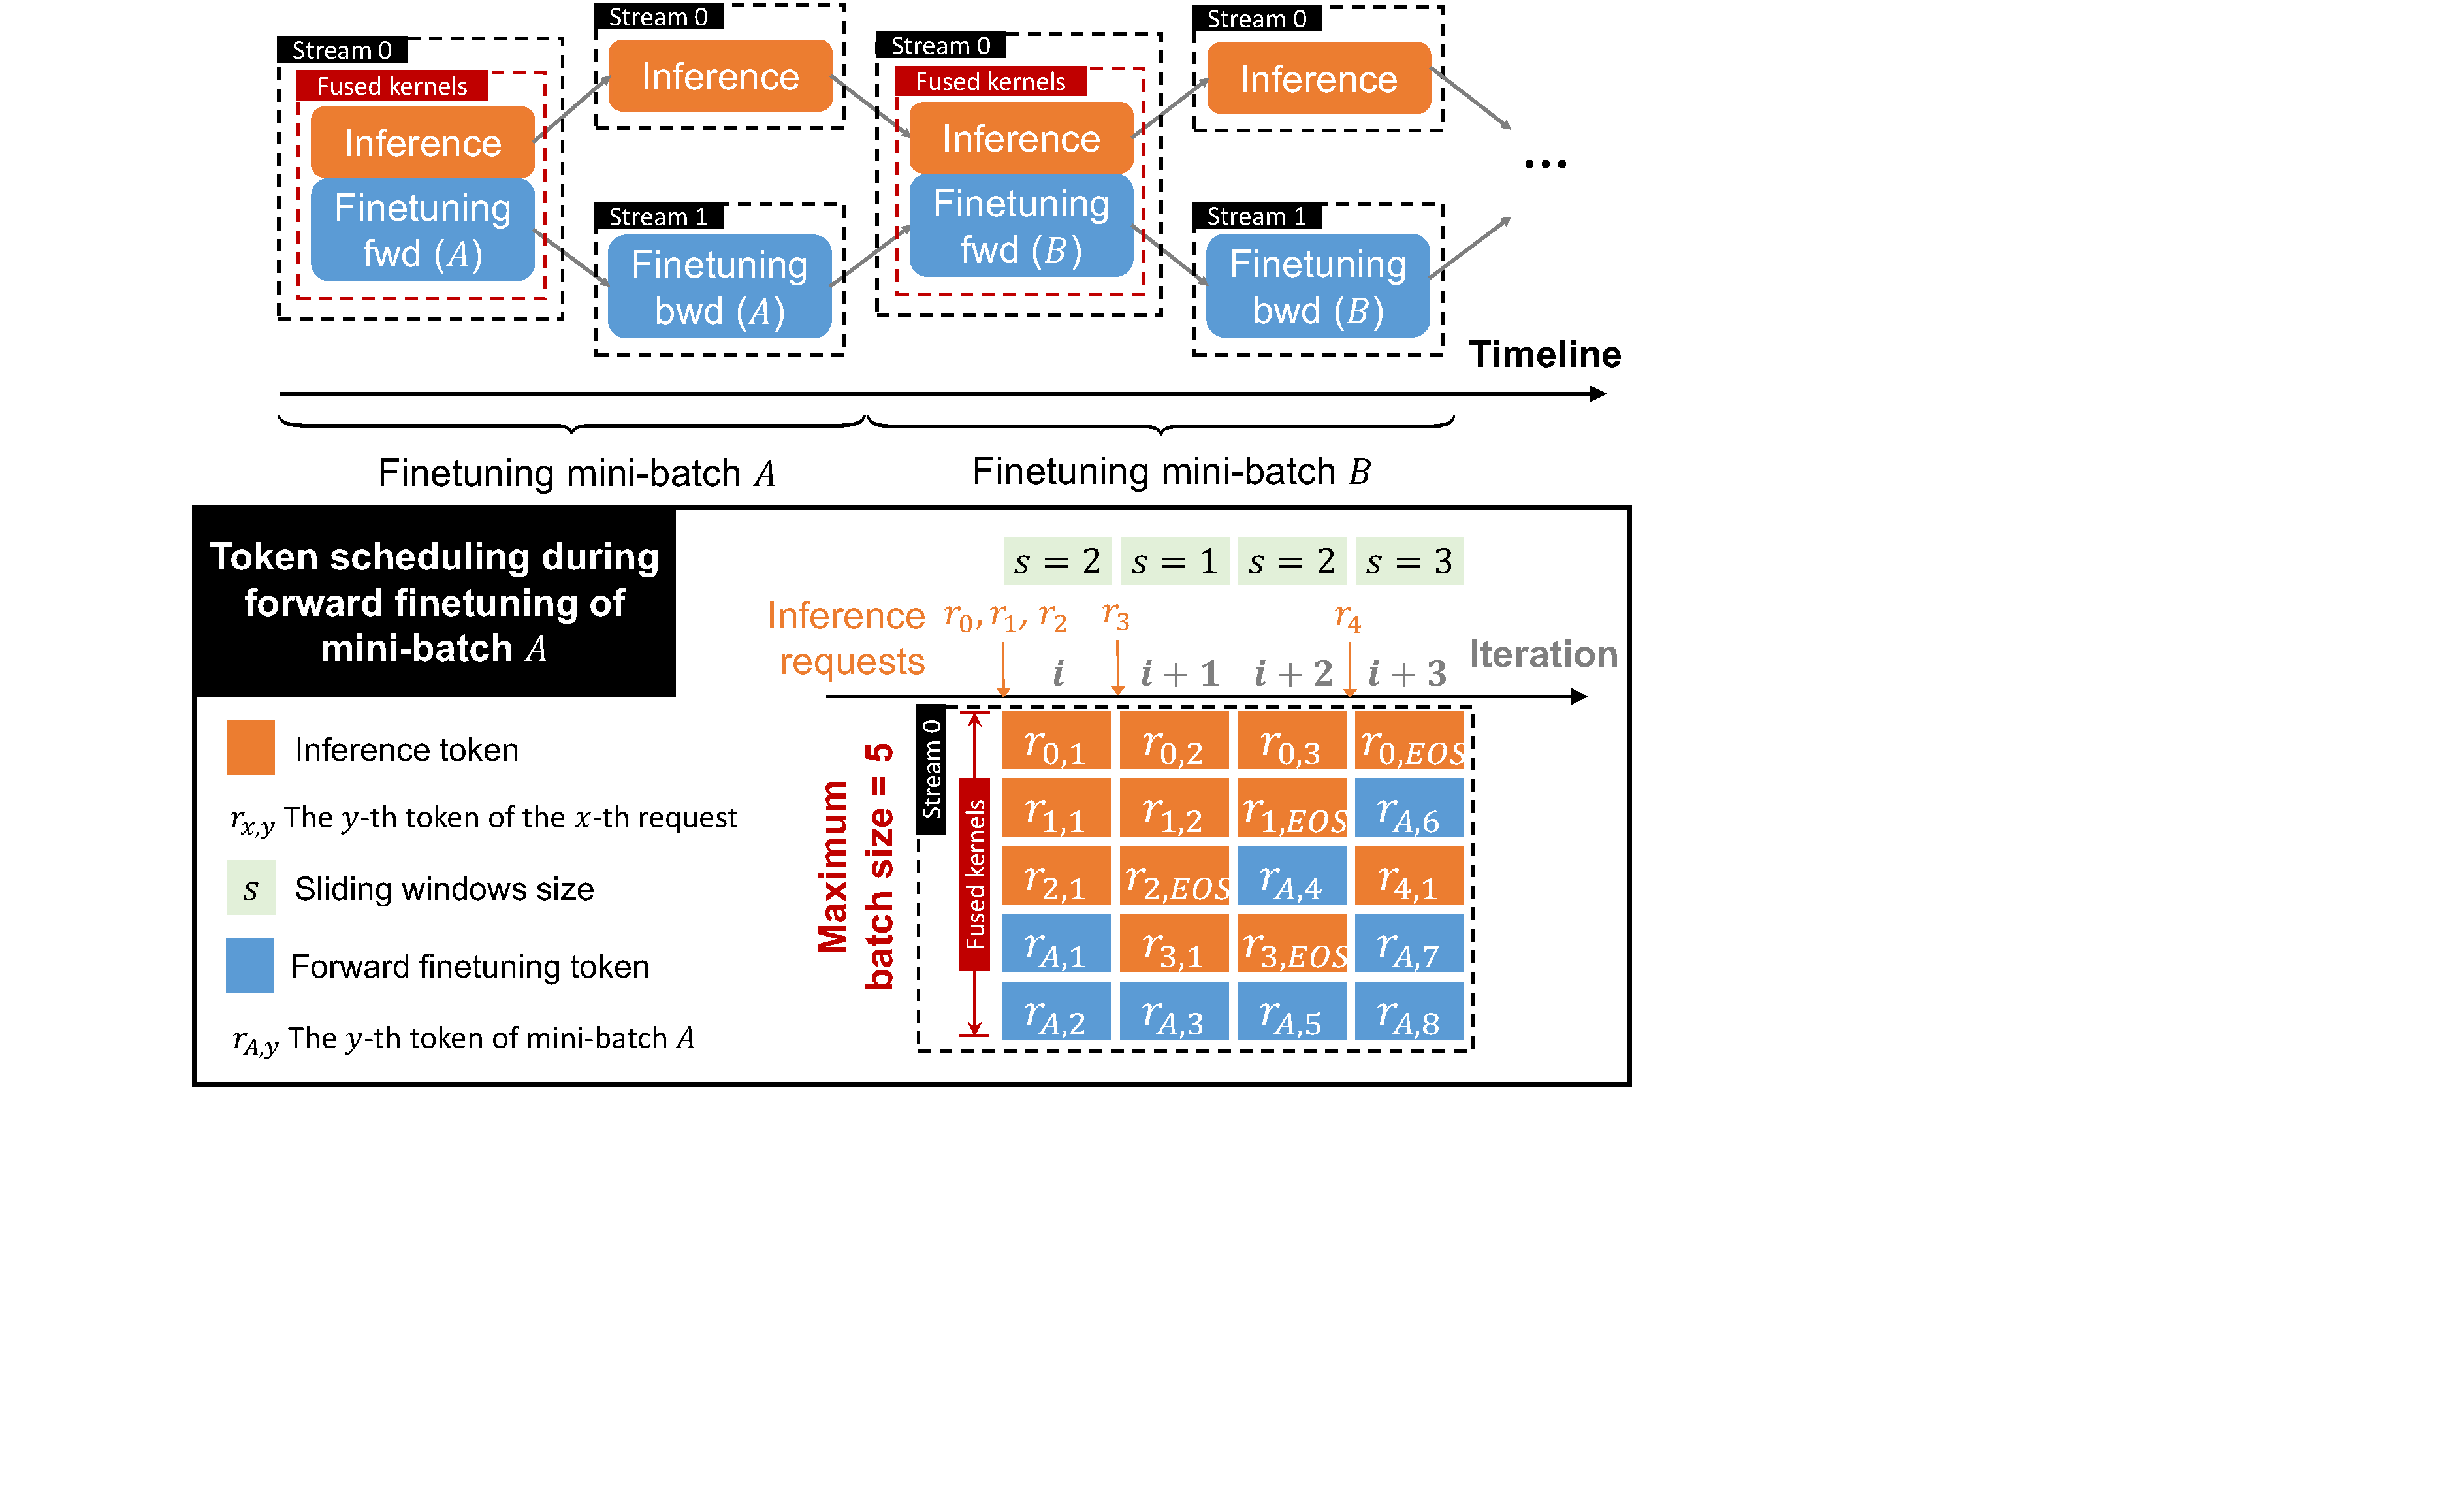
\includegraphics[width=0.8\linewidth]{figures/flexllm/token_level_scheduling4.pdf}
    \caption{Execution timeline and token scheduling when co-serving inference requests and a finetuning mini-batch.}
    \label{flexllm:fig:execution_timeline}
\end{figure}

\subsection{Hybrid Token Scheduler}
\label{flexllm:subsec:scheduler}

\FlexLLM's \textit{hybrid token scheduler} coordinates token-level GPU execution in two stages.
%
First, \FlexLLM determines the scheduling of available inference requests based on specific scheduling policies. By default, \FlexLLM adopts Orca's \textit{iteration-level scheduling}~\cite{yu2022orca}, which maintains a fixed maximum batch size and dynamically replaces each completed request with a new one whenever available.
%
To further mitigate blocking caused by long input sequences, \FlexLLM incorporates the chunked-prefill optimization~\cite{agrawal2024taming}.

Second, after determining the inference schedule for a given iteration, \FlexLLM opportunistically appends as many finetuning tokens as possible---determined by the sliding window size $s$---to maximize GPU utilization. The number of finetuning tokens added is determined automatically using the formula $s=\operatorname*{arg\,max}_s f(c, s)\leq$ SLO, where $f(\cdot, \cdot)$ is the latency estimation function and $c$ is the number of inference tokens scheduled in the current iteration. Here $f(\cdot, \cdot)$ is derived via offline profiling of the LLM's execution~\cite{narayanan2023cheaply}.
%
Such a window-based, best-effort scheduling mechanism ensures that \FlexLLM can automatically adapt to inference workload fluctuations, maintaining inference SLOs while opportunistically allocating compute to finetuning tasks (\Cref{flexllm:sec:exp:dynamic}).

\Cref{flexllm:fig:execution_timeline} illustrates the execution timeline of \FlexLLM and shows an example of a token scheduling plan for a finetuning mini-batch $A$, under a representative inference request arrival pattern (i.e., $r_0$ to $r_4$).
To preserve the semantics of finetuning, \FlexLLM enforces the execution dependencies between the forward and backward passes of each mini-batch.
During the forward pass, \FlexLLM leverages fused GPU kernels to jointly process both inference and finetuning tokens. This approach avoids additional kernel launch overhead and is enabled by the shared token-wise computation logic between inference and finetuning. In particular, finetuning tokens follow the same execution pattern and causal masking rules as inference tokens during the prefill phase, guaranteeing compatibility at the kernel level.
For the backward pass, \FlexLLM adopts a space-sharing approach, using two separate GPU streams: one for inference tokens and another for finetuning tokens. This design allows concurrent execution without interference.

\subsection{Preventing Tenant Interference with Virtual Token Counters}
\label{flexllm:sec:vtc-integration}

\FlexLLM can prevent tenant interference (e.g., noisy neighbor problems) thanks to the Virtual Token Counter (VTC) algorithm~\cite{sheng2024fairness}, which can be combined with our co-serving scheduler. This integration ensures fair resource allocation across tenants while maintaining high GPU utilization.

In multi-tenant PEFT serving, tenants may submit requests at vastly different rates. Without fairness controls, aggressive tenants can monopolize resources and degrade service for others. VTC addresses this by tracking per-tenant service consumption and prioritizing underserved tenants.

\Cref{flexllm:alg:flexllm-vtc} shows the integration of VTC into \FlexLLM's token-level scheduling. Key modifications include: (1) per-tenant virtual counters $c_i$ tracking cumulative service, (2) counter lifting when idle tenants rejoin to prevent unfair credit accumulation, (3) fair selection of both inference and finetuning tokens based on minimum counter values, and (4) weighted counter updates reflecting different costs of input ($w_p$), output ($w_q$), and finetuning ($w_r$) tokens.

The integration guarantees bounded fairness across tenants. In the analysis, finetuning requests are treated as a special case of inference requests, allowing us to directly apply results from the Virtual Token Counter analysis~\cite{sheng2024fairness}. Let $W_i(t_1, t_2)$ denote the weighted service received by tenant $i$ and $M$ be the maximum number of tokens. The following lemma and theorems formalize the fairness bounds.

\begin{lemma}
When $Q \neq \emptyset$,
\begin{equation}\label{flexllm:eq:vtc}
    \max_{i \in Q} c_i - \min_{i \in Q} c_i \le \max(w_p \cdot L_{\text{input}}, \max(w_q, w_r) \cdot M).
\end{equation}
\end{lemma}

\begin{theorem}[Fairness for overloaded tenants]
    For any tenants $f$ and $g$, for any time interval $[t_1,t_2)$ in which $f$ and $g$ are backlogged, \Cref{flexllm:alg:flexllm-vtc} guarantees
\[
    |W_f(t_1, t_2) - W_g(t_1, t_2)| \leq 2\max(w_p \cdot L_{\text{input}}, \max(w_q, w_r) \cdot M).
\]
\end{theorem}

\begin{theorem}[Fairness for non-overloaded tenants]
    Let $[t_1, t_2)$ be any time interval, $T(t,t_2)$ be the total services received for all tenants during $[t,t_2)$, $n(t,t_2)$ be the number of tenants that have requested services during the interval, and $U$ be the upper bound from \Cref{flexllm:eq:vtc}.

    Assume a tenant $f$ is not backlogged at $t_1$ and has requested services less than $\frac{T(t,t_2)}{n(t,t_2)}-5U$ during $[t_1, t_2)$. Then, all of the services requested from $f$ during the interval $[t_1,t_2)$ will be dispatched.
\end{theorem}

The algorithm remains work-conserving---idle resources are allocated to active tenants---while preventing any single tenant from monopolizing the system. The overhead is minimal: $O(n)$ counters for $n$ tenants, with updates occurring at \FlexLLM's existing token-level granularity. This integration preserves \FlexLLM's memory optimizations (dependent parallelization, graph pruning) while adding fairness guarantees essential for multi-tenant deployments.

\begin{algorithm}[htbp]
\caption{\FlexLLM with Virtual Token Counter for fair co-serving.}
\label{flexllm:alg:flexllm-vtc}
\begin{algorithmic}[1]
\State \textbf{Input:} Input weight $w_p$, output weight $w_q$, finetuning weight $w_r$, max tokens $M$
\State \textbf{Initialize:} $B \leftarrow \emptyset$, $c_i \leftarrow 0$ for all tenants $i$, $Q \leftarrow \emptyset$
\State
\flexllmLeftComment{Monitoring Stream}
\While{True}
    \If{request $r$ from tenant $u$ arrives}
        \If{$\not\exists r' \in Q, \mathit{tenant}(r') = u$}
            \If{$Q = \emptyset$}
                \State $l \gets$ the last tenant that left $Q$
                \State $c_u \gets \max\{c_u, c_l\}$
            \Else
                \State $c_u \gets \max\{c_u, \min\{c_i \mid i \in Q\}\}$
            \EndIf
        \EndIf
        \State $Q_u \leftarrow Q_u \cup \{r\}$
    \EndIf
\EndWhile
\State
\flexllmLeftComment{Execution Stream}
\While{True}
    \If{can\_add\_new\_requests()}
        \flexllmLeftComment{Fair inference selection}
        \While{memory available for inference}
            \State $k \leftarrow \arg\min_{i \in \{\mathit{tenant}(r) \mid r \in Q \text{ is an inference task}\}} c_i$
            \State $r \gets$ the earliest inference request in $Q$ from $k$
            \State Add inference request from $Q_k$ to batch $B$
            \State $c_k \leftarrow c_k + w_p \cdot \text{input\_length}(r)$
        \EndWhile
        \flexllmLeftComment{Fair finetuning token selection}
        \State $s \leftarrow$ compute\_finetuning\_window()
        \While{$s > 0$ and memory available}
            \State $k \leftarrow \arg\min_{i \in \{\mathit{tenant}(r) \mid r \in Q \text{ is a finetuning task}\}} c_i$
            \State $t \gets \min(s, \text{available})$
            \State Process next $t$ tokens from tenant $k$
            \State $c_k \gets c_k + w_r \cdot t$
            \State $s \leftarrow s - t$
        \EndWhile
    \EndIf
    \State Execute decode step for $B$
    \For{each tenant $i$ with tokens generated}
        \State $c_i \leftarrow c_i + w_q \cdot \text{output\_tokens}_i$
    \EndFor
\EndWhile
\end{algorithmic}
\end{algorithm}

\section{Implementation}
\label{flexllm:sec:impl}
\FlexLLM is built on FlexFlow Serve~\cite{specinfer} with 9K lines of C++ and CUDA code. It provides C++ and Python bindings, with full HuggingFace compatibility for the \texttt{PEFT}~\cite{peft} and \texttt{transformers}~\cite{transformers} libraries. \FlexLLM supports PEFT models with LLaMA~\cite{touvron2023llama}, GPT~\cite{brown2020language}, OPT~\cite{zhang2022opt}, Falcon~\cite{falcon40b}, or MPT~\cite{MosaicML2023Introducing} backbones, among others.

\paragraph{Memory management.}
\FlexLLM manages the required GPU memory using a combination of static and dynamic allocation. Static allocation reserves GPU space for the backbone weights and the KV cache required for incremental decoding during inference. Dynamic allocation is used for gradients, activations, and optimizer states. When a finetuning request is received, \FlexLLM allocates memory during the first forward pass and reuses it during subsequent backward passes, freeing up space when it is no longer needed.
For inference memory management, \FlexLLM employs paged attention~\cite{vllm} with chunked prefill~\cite{agrawal2023sarathi} to dynamically allocate KV cache pages and minimize evictions. New inference requests are only admitted if the entire prompt can fit within available KV cache pages, preventing memory fragmentation and ensuring stable inference performance during co-serving.

\begin{figure}[htbp]
    \centering
    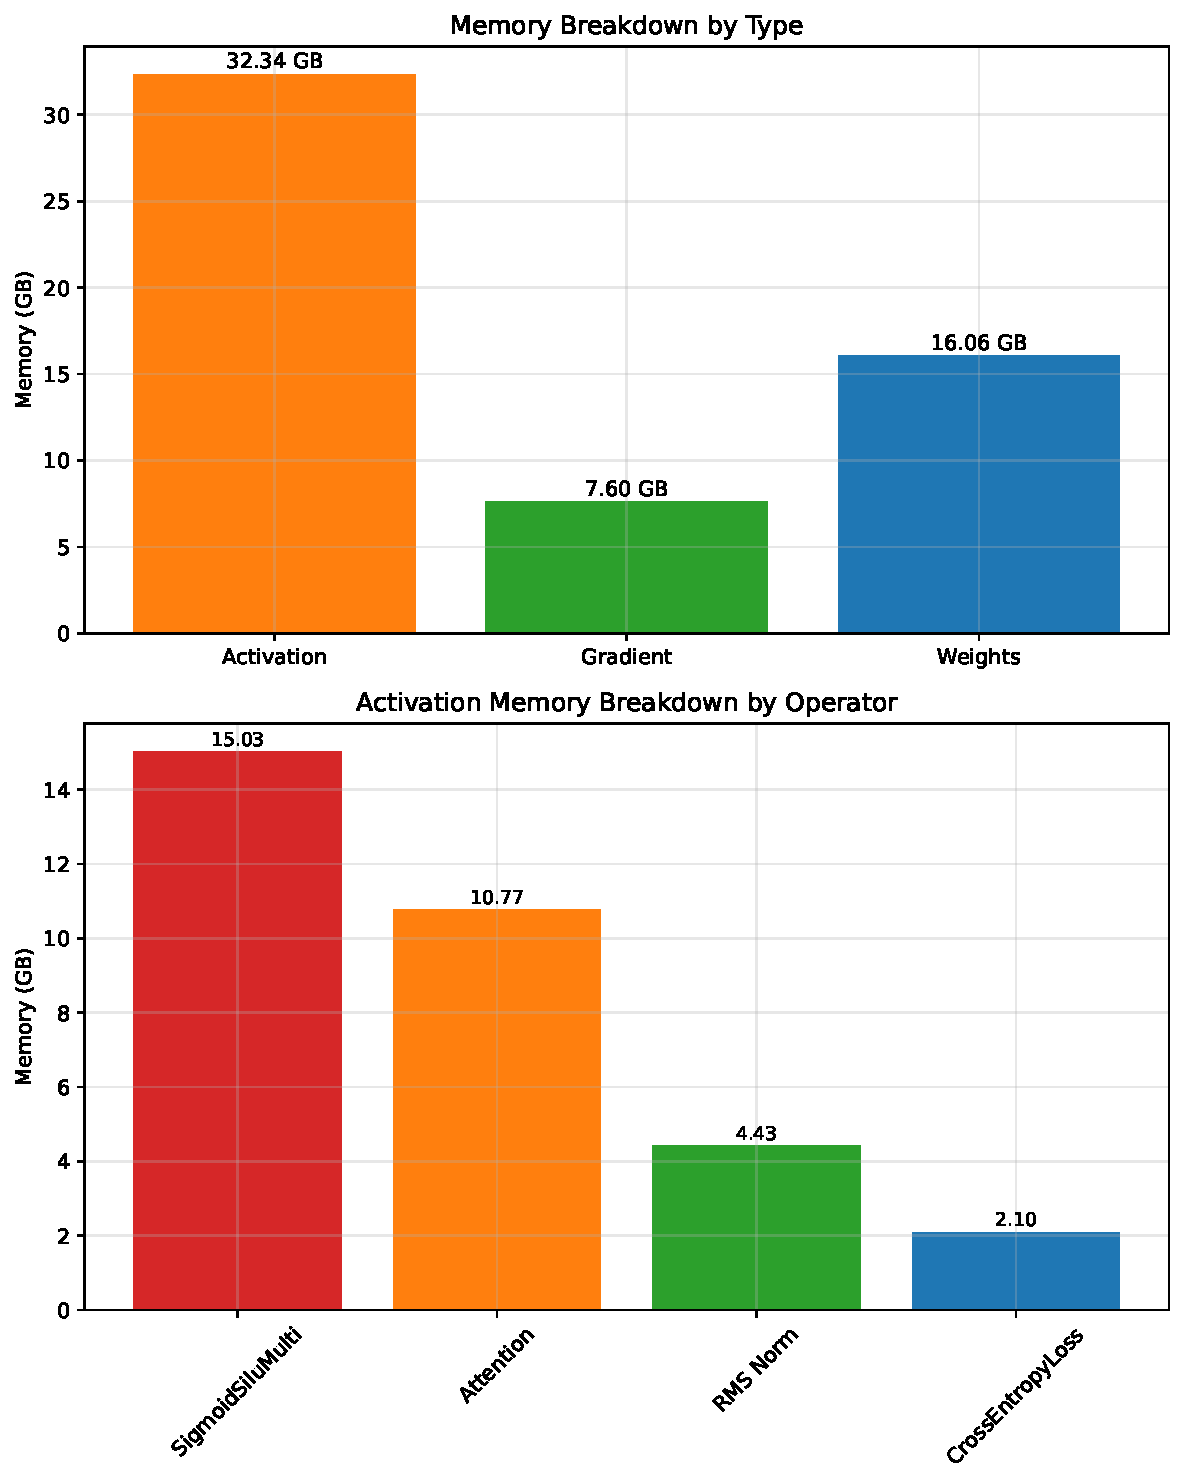
\includegraphics[width=0.75\linewidth]{figures/flexllm/memory_breakdown.pdf}
    \caption{Component-wise memory breakdown for \FlexLLM co-serving LLaMA-3.1-8B with LoRA finetuning.}
    \label{flexllm:fig:memory-breakdown-detailed}
\end{figure}

\paragraph{Finetuning memory budget.}
\Cref{flexllm:fig:memory-breakdown-detailed} shows the component-wise memory breakdown for \FlexLLM co-serving LLaMA-3.1-8B with LoRA rank 16. For finetuning memory management, \FlexLLM preallocates a fixed budget sufficient for the largest supported PEFT configuration (maximum rank with all target modules enabled). This budget covers PEFT weights, gradients, optimizer momentum values, and low-rank activations. The static allocation strategy prevents memory fragmentation during dynamic co-serving while ensuring deterministic memory bounds regardless of the specific PEFT configurations being served.

\paragraph{Key-value gradient accumulator.}
To support token-level finetuning, it is necessary to accumulate key-value gradients for every preceding token in a given sequence during backpropagation. \FlexLLM utilizes static allocation to reserve space for key-value gradient accumulation. During backpropagation, the gradients for keys and values of a specific segment are obtained, and the position of this segment in the overall sequence is determined. \FlexLLM then accumulates the new key-value gradients of all subsequently scheduled segments. When a segment is scheduled during backpropagation, it includes accumulated gradients from future tokens.

\section{Evaluation}
\label{flexllm:sec:eval}

\begin{figure}[htbp]
    \centering
    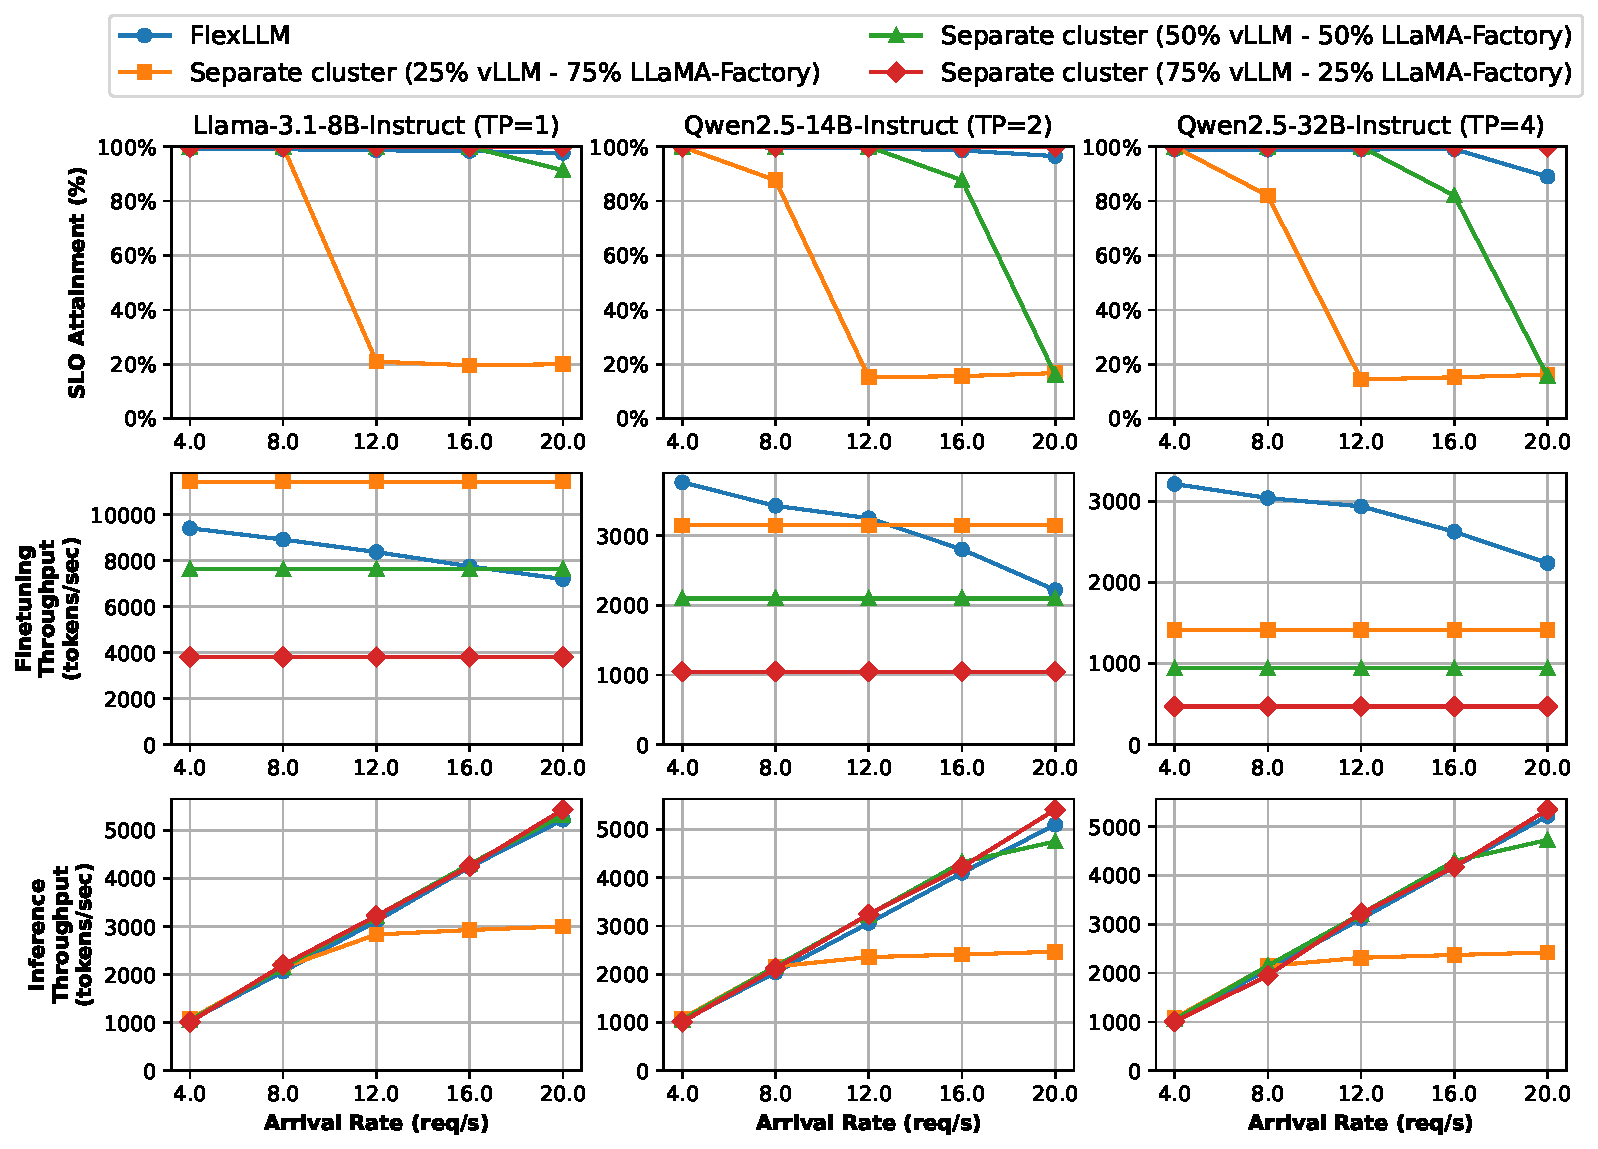
\includegraphics[width=\linewidth]{figures/flexllm/combined_plot.pdf}
    \caption{End-to-end comparison between co-serving and using separate resources on three models.}
    \label{flexllm:fig:end-to-end}
\end{figure}

\begin{figure}[htbp]
    \centering
    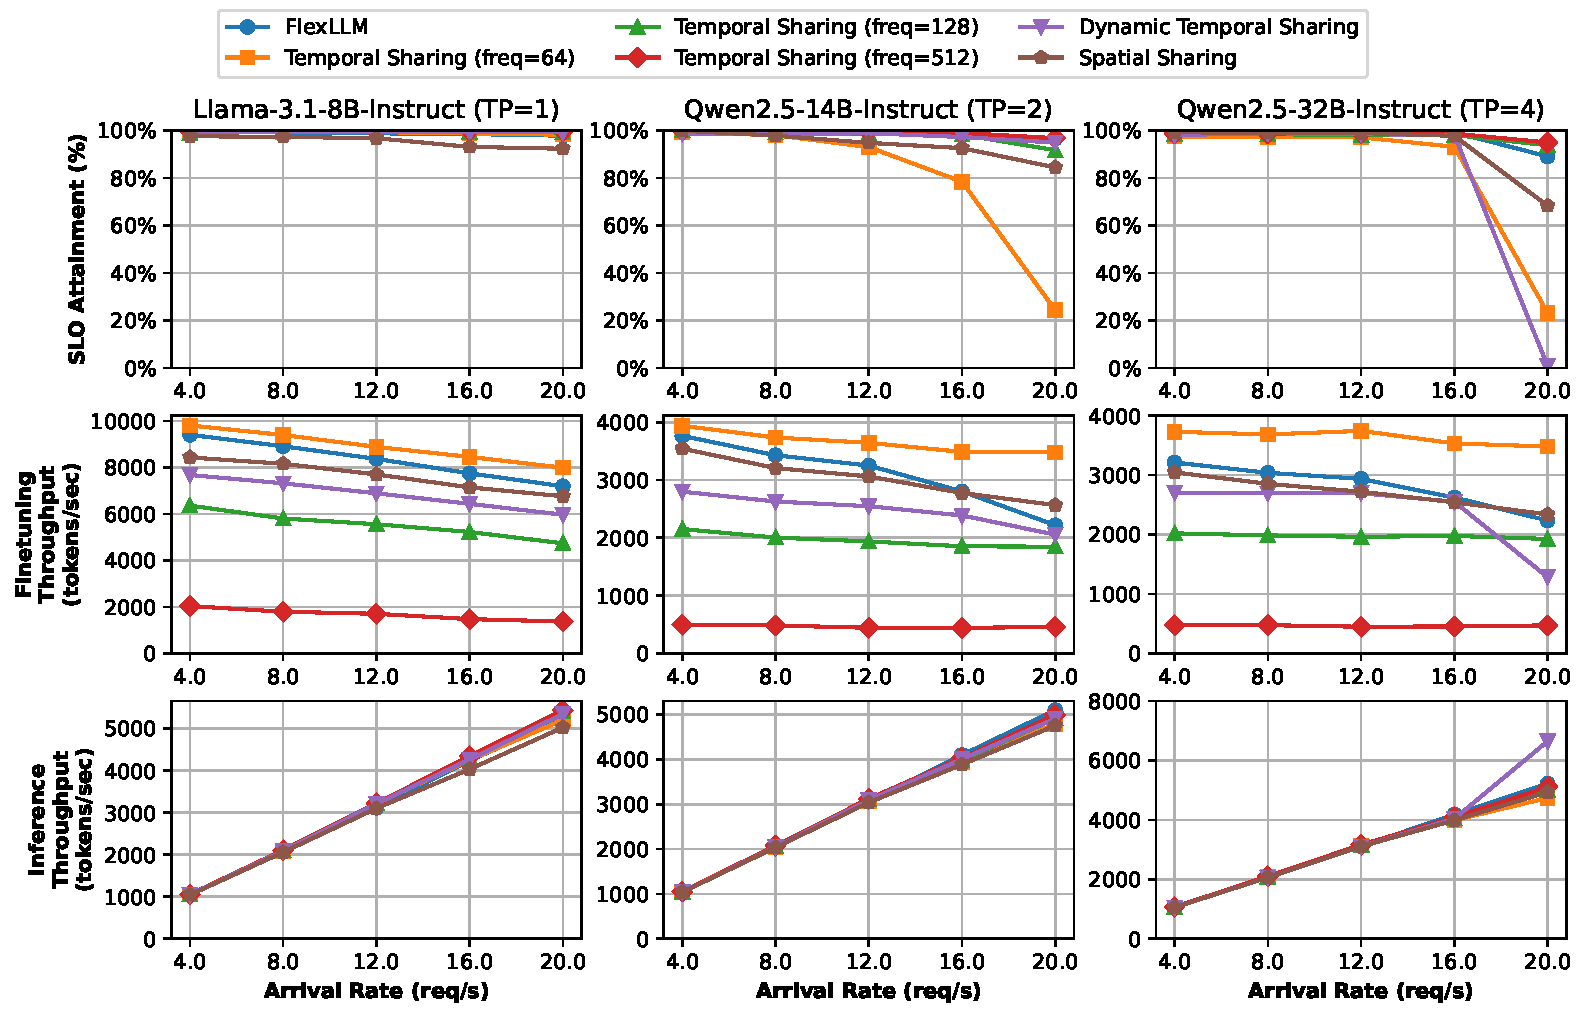
\includegraphics[width=\linewidth]{figures/flexllm/internal_baselines.pdf}
    \caption{End-to-end comparison of co-serving with temporal and spatial sharing strategies.}
    \label{flexllm:fig:temporal-spatial-sharing}
\end{figure}

\paragraph{LLMs and PEFT models.} We evaluated \FlexLLM across three publicly available LLMs: LLaMA-3.1-8B~\cite{llama2}, Qwen-2.5-14B~\cite{qwen2025qwen25technicalreport}, and Qwen-2.5-32B~\cite{qwen2025qwen25technicalreport} from HuggingFace~\cite{huggingfacemodels}.
Since existing LLM serving systems only support base models and LoRA-based PEFT, we focus on these configurations for fair comparison.
We applied LoRA with rank 16 to MLP down projection layers, yielding 9.4M, 14.5M, and 25.16M trainable parameters respectively.

\paragraph{Platform.} Experiments were performed on Perlmutter~\cite{perlmutter} nodes with AMD EPYC 7763 processors, 256\,GB DRAM, and four NVIDIA A100-SXM4-80GB GPUs connected via HPE Slingshot (200\,Gb/s). We used tensor-model parallelism for LLM serving and finetuning.

\paragraph{Workload.}
We synthesized inference workloads using ShareGPT~\cite{sharegpt} prompt/generation lengths and Azure ChatGPT production traces~\cite{burstgpt} for realistic arrival patterns, following recent work~\cite{vllm,zhong2024distserve,agrawal2023sarathi,nanoflow,pipellm,medusa}. The original trace spans multiple days and captures real production arrival patterns from ChatGPT serving on Azure OpenAI, providing realistic inference workload characteristics including bursty request arrivals and varying concurrency patterns.  We sampled 20-minute intervals, adjusting the arrival times to simulate different average arrival rates.
We set TPOT SLOs to 50ms (8B model) and 75ms (14B/32B models) following the methodology from prior work~\cite{agrawal2023sarathi}, with 5s maximum TTFT to prevent excessive queueing.

We sampled each finetuning request from the \texttt{Sky-T1\_data\_17k} dataset~\cite{novasky2025dataset}, used to finetune the \texttt{Sky-T1-32B-Preview} reasoning model~\cite{novasky2025model}, a finetuned Qwen2.5 variant with performance comparable to OpenAI's o1-preview~\cite{o1-preview} on math and coding benchmarks. We truncated sequences to 8192 tokens and used the Adam optimizer~\cite{kingma2014adam}.

\subsection{End-to-end Comparison}
\label{flexllm:sec:exp:e2e}

We compare \FlexLLM's co-serving approach with existing approaches that employ separate clusters for inference and finetuning tasks. In the separate cluster approach, we use vLLM~\cite{vllm} and LlamaFactory~\cite{llamafactory} as the inference and finetuning systems, respectively, as they represent state-of-the-art solutions for these workloads. We selected vLLM over alternatives like DeepSpeed-MII~\cite{deepspeed-mii} and TensorRT-LLM~\cite{tensorrt-llm} because recent vLLM optimizations have closed previous performance gaps, while PipeSwitch~\cite{bai2020pipeswitch} lacks support for autoregressive LLM generation. We enable all available optimizations, including \texttt{torch.compile} and chunked prefills for vLLM v1; DeepSpeed ZeRO Stage 3, Unsloth and FlashAttention for LlamaFactory.
We allocated 4, 8, and 16 A100 GPUs for the three models respectively.

\Cref{flexllm:fig:end-to-end} shows the results. The separate approach uses tensor parallelism (degree 1, 2, 4) for the three models respectively, creating four pipelines in total. We explored various strategies to distribute resources between inference and finetuning tasks. Configurations like 25\% vLLM -- 75\% LlamaFactory allocate 25\% of resources (i.e., 1 pipeline) to inference, 75\% (i.e., 3 pipelines) to finetuning.

Configurations with fewer inference pipelines (25\%--50\% vLLM) handle only lightweight workloads, achieving limited inference throughput and SLO attainment under more intensive workloads. Dedicating more pipelines to inference (75\% vLLM) maintains high SLO attainment but reduces finetuning throughput.

\FlexLLM maintains near-optimal SLO attainment without compromising finetuning performance by prioritizing latency-sensitive inference and opportunistically maximizing finetuning tokens.

Across all three models, \FlexLLM matches the 75\% vLLM -- 25\% LlamaFactory configuration in inference SLO attainment (at or above 90\% even at 20 req/s) and inference throughput, while dramatically improving finetuning throughput. Specifically, under heavy inference loads (20 req/s), \FlexLLM sustains finetuning throughputs of 7.2K, 2.2K and 2.2K tokens/s for LLaMA-3.1-8B, Qwen-2.5-14B, and Qwen-2.5-32B respectively, compared to only 3.8K, 1.0K, and 0.5K tokens/s in the 75\% vLLM -- 25\% LlamaFactory setup, i.e., a \textbf{1.9$\times$--4.8$\times$} improvement. Under light inference loads (4.0 req/s), \FlexLLM sustains finetuning throughputs of 9.4K, 3.7K, and 3.2K tokens/s for the same models, translating to a \textbf{2.5$\times$--6.8$\times$} improvement over the 75\% vLLM -- 25\% LlamaFactory setup.

\subsection{GPU Scheduling}
\label{flexllm:sec:exp:scheduling}

This section compares \FlexLLM's co-serving mechanism with two commonly used GPU scheduling strategies: {\em temporal sharing} and {\em spatial sharing}.
Temporal sharing interleaves the execution of inference and finetuning tasks over time, as illustrated in \Cref{flexllm:fig:baseline}. Spatial sharing simultaneously launches inference and finetuning computations using separate CUDA resources. Both strategies are implemented on top of \FlexLLM by replacing the co-serving mechanism with their respective scheduling strategies. To ensure a fair comparison, all memory optimizations are enabled in each baseline.

\Cref{flexllm:fig:temporal-spatial-sharing} shows the results. For temporal sharing, interleaving one inference iteration with one finetuning iteration would violate the SLOs for nearly all inference requests.
This is because each inference iteration is expected to complete within tens of milliseconds, whereas a finetuning iteration requires several seconds. To mitigate this issue, in the temporal sharing experiments, we interleave each finetuning iteration with $n$ inference iterations, where $n$ is the inference frequency shown in the figure.

While adopting a low inference frequency in temporal sharing (i.e., frequency = 64) maximizes finetuning throughput, it adversely impacts the SLO attainment and throughput for inference requests.
Employing a frequency of 128 enables temporal sharing to match the inference throughput and SLO attainment rate of co-serving. However, it also reduces finetuning throughput by 0.57$\times$--0.86$\times$ compared to co-serving.

Finally, we also implemented a dynamic temporal sharing baseline (described below), where the interleaving frequency is determined dynamically based on queue lengths, batch sizes, arrival rates, and completion rates.
Dynamic temporal sharing outperforms fixed-frequency temporal sharing by adapting to workload conditions, maintaining SLO attainment above 90\% in most scenarios, and achieving impressive inference throughputs of 5.4K, 4.9K, and 6.6K tokens/s for the three models under heavy loads (20 req/s). However, it still lags behind co-serving, whose finetuning throughput is \textbf{1.0--1.7$\times$} higher, and shows instability under the heaviest loads as SLO attainment drops significantly for the 32B model.

Spatial sharing allocates separate GPU resources for inference and finetuning, achieving comparable finetuning throughput to co-serving. However, it remains suboptimal in SLO attainment under heavy inference workloads due to the interference between inference and finetuning tasks.

\paragraph{Dynamic temporal sharing baseline.}
\label{flexllm:sec:dts-appendix}
Dynamic Temporal Sharing (DTS) is an adaptive baseline that dynamically adjusts the frequency of switching between inference and finetuning phases based on real-time system conditions. The algorithm (\Cref{flexllm:alg:dts}) continuously monitors queue lengths, batch sizes, arrival rates, and completion rates to compute a multi-dimensional pressure metric comprising queue pressure ($\text{avg\_queue}/20.0$), spike pressure ($\text{max\_queue}/25.0$), and backlog pressure ($(\text{arrival\_rate} - \text{completion\_rate})/8.0$). Based on the total pressure, DTS adaptively selects finetuning intervals between 64--512 steps using pressure thresholds (pressure $\leq 0.8$ for minimum frequency, pressure $\geq 2.0$ for maximum frequency) and linear interpolation with a $0.6\times$ scaling factor for intermediate values. To ensure system stability, the algorithm incorporates hysteresis through weighted historical averaging ($(\text{frequency} + 2 \times \text{prev\_frequency})/3$), applies stabilization adjustments to computed frequencies, and implements decision delays where frequency recomputation occurs only every third scheduling decision to prevent oscillatory behavior under varying workloads.

\begin{algorithm}[htbp]
\caption{Dynamic temporal sharing (DTS) baseline.}
\label{flexllm:alg:dts}
\begin{algorithmic}[1]
\Require $q$, $b$, $a$, $c$
\State $Q[]$, $B[]$, $r_a$, $r_c$
\State $s$, $f_p$, $d$
\Procedure{Scheduler\_Step}{$q$, $b$, $a$, $c$}
    \State $r_a \leftarrow r_a + a$
    \State $r_c \leftarrow r_c + c$
    \State $Q$.append($q$)
    \State $B$.append($b$)
    \State $s \leftarrow s - 1$
    \If{$s \leq 0$}
        \State $d \leftarrow d + 1$
        \If{$d \geq 3$}
            \State $s \leftarrow$ \Call{Compute\_Next\_Interval}{}
            \State $d \leftarrow 0$
        \Else
            \State $s \leftarrow \min(512, f_p \times 1.1)$
        \EndIf
        \State \Call{Reset\_Stats}{}
        \State \Return True \Comment{switch to finetuning}
    \EndIf
    \State \Return False \Comment{continue inference}
\EndProcedure
\Procedure{Compute\_Next\_Interval}{}
    \If{$Q$.empty()}
        \State \Return 64
    \EndIf
    \State $\bar{q} \leftarrow$ mean($Q$)
    \State $q_{max} \leftarrow$ max($Q$)
    \State $\bar{b} \leftarrow$ mean($B$)
    \State $\lambda \leftarrow r_a / |Q|$
    \State $\mu \leftarrow r_c / |Q|$
    \State $p_q \leftarrow \min(1.0, \bar{q} / 20.0)$
    \State $p_s \leftarrow \min(0.5, q_{max} / 25.0)$
    \State $p_b \leftarrow \max(0.0, (\lambda - \mu) / 8.0)$
    \State $p \leftarrow p_q + p_s + p_b$
    \If{$p \leq 0.8$}
        \State $f \leftarrow 64$
    \ElsIf{$p \geq 2.0$}
        \State $f \leftarrow 512$
    \Else
        \State $p_n \leftarrow (p - 0.8) / 1.2$
        \State $f \leftarrow 64 + p_n \times 0.6 \times (512 - 64)$
    \EndIf
    \State $f \leftarrow f \times 1.35$ \Comment{stabilization adjustment}
    \State $f_s \leftarrow (f + 2 \times f_p) / 3$
    \State $f_p \leftarrow f_s$
    \State $f_s \leftarrow \max(f_s, 64 + 16)$
    \State \Return clamp($f_s$, 64, 512)
\EndProcedure
\end{algorithmic}
\end{algorithm}

\begin{figure}[htbp]
    \centering
    \begin{subfigure}[t]{0.75\linewidth}
      \centering
      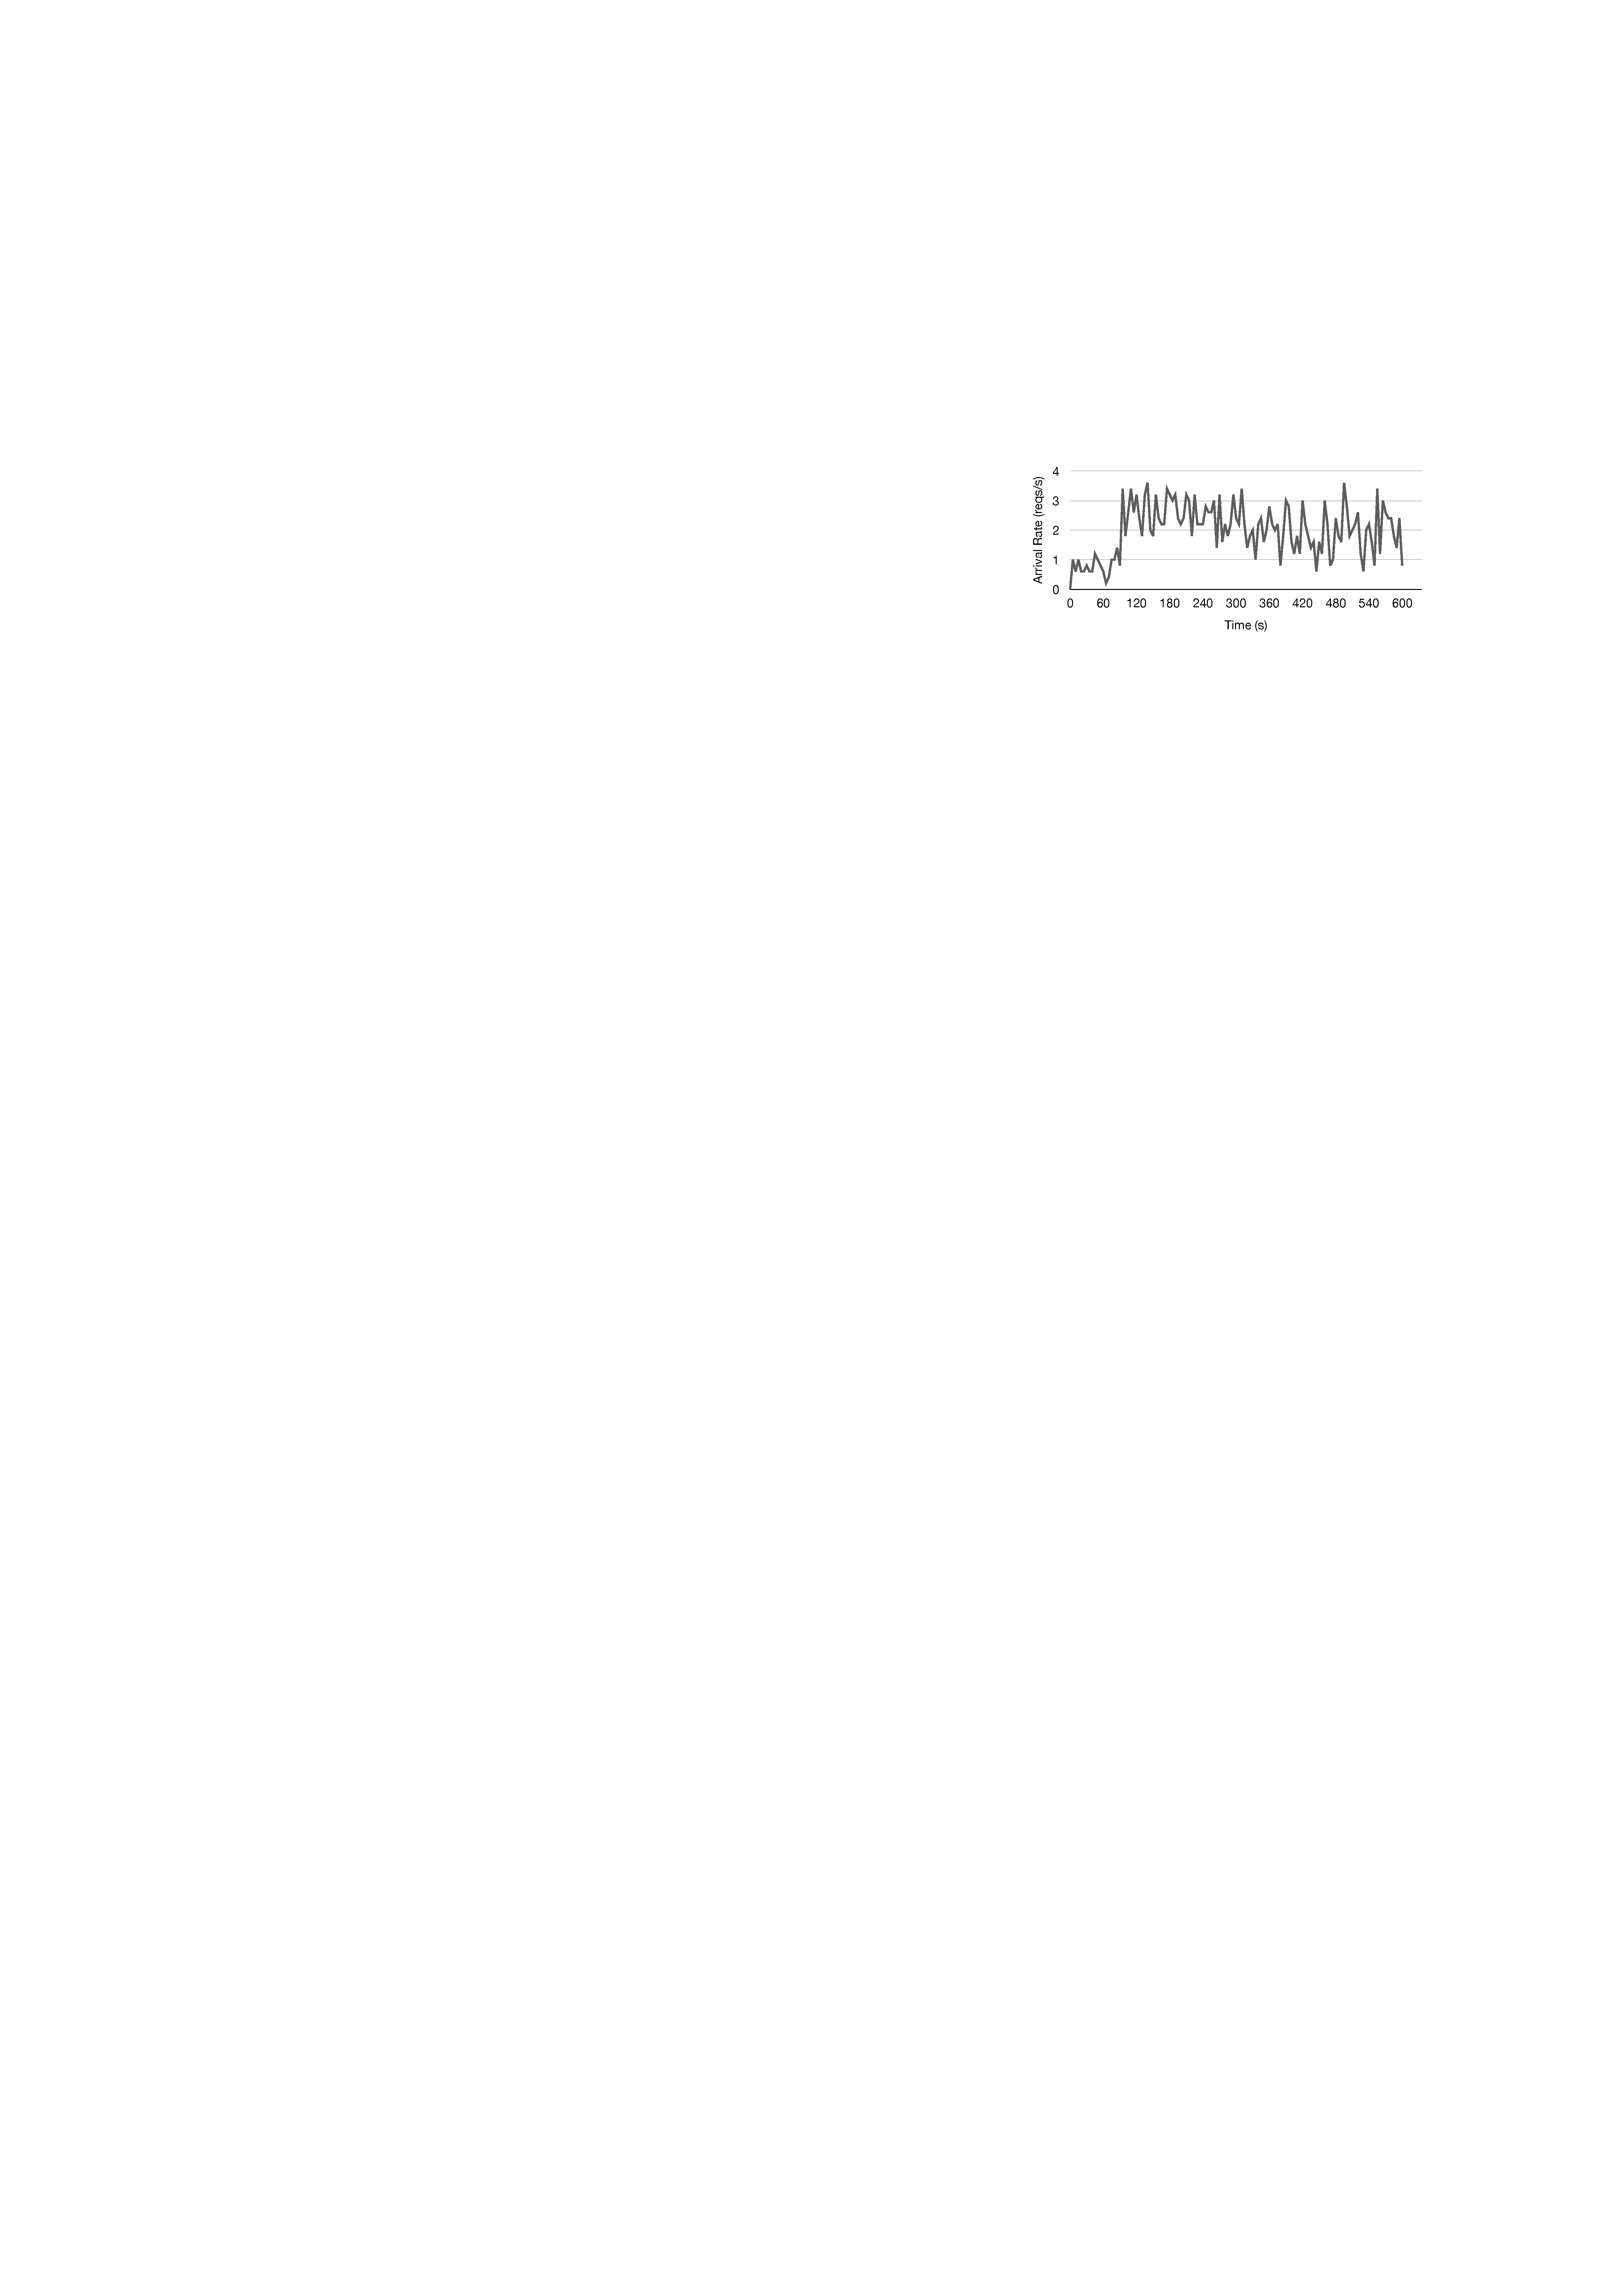
\includegraphics[width=\linewidth]{figures/flexllm/case_arrival.pdf}
      \caption{Arrival of inference requests}
    \end{subfigure}\\[1ex]
    \begin{subfigure}[t]{0.75\linewidth}
      \centering
      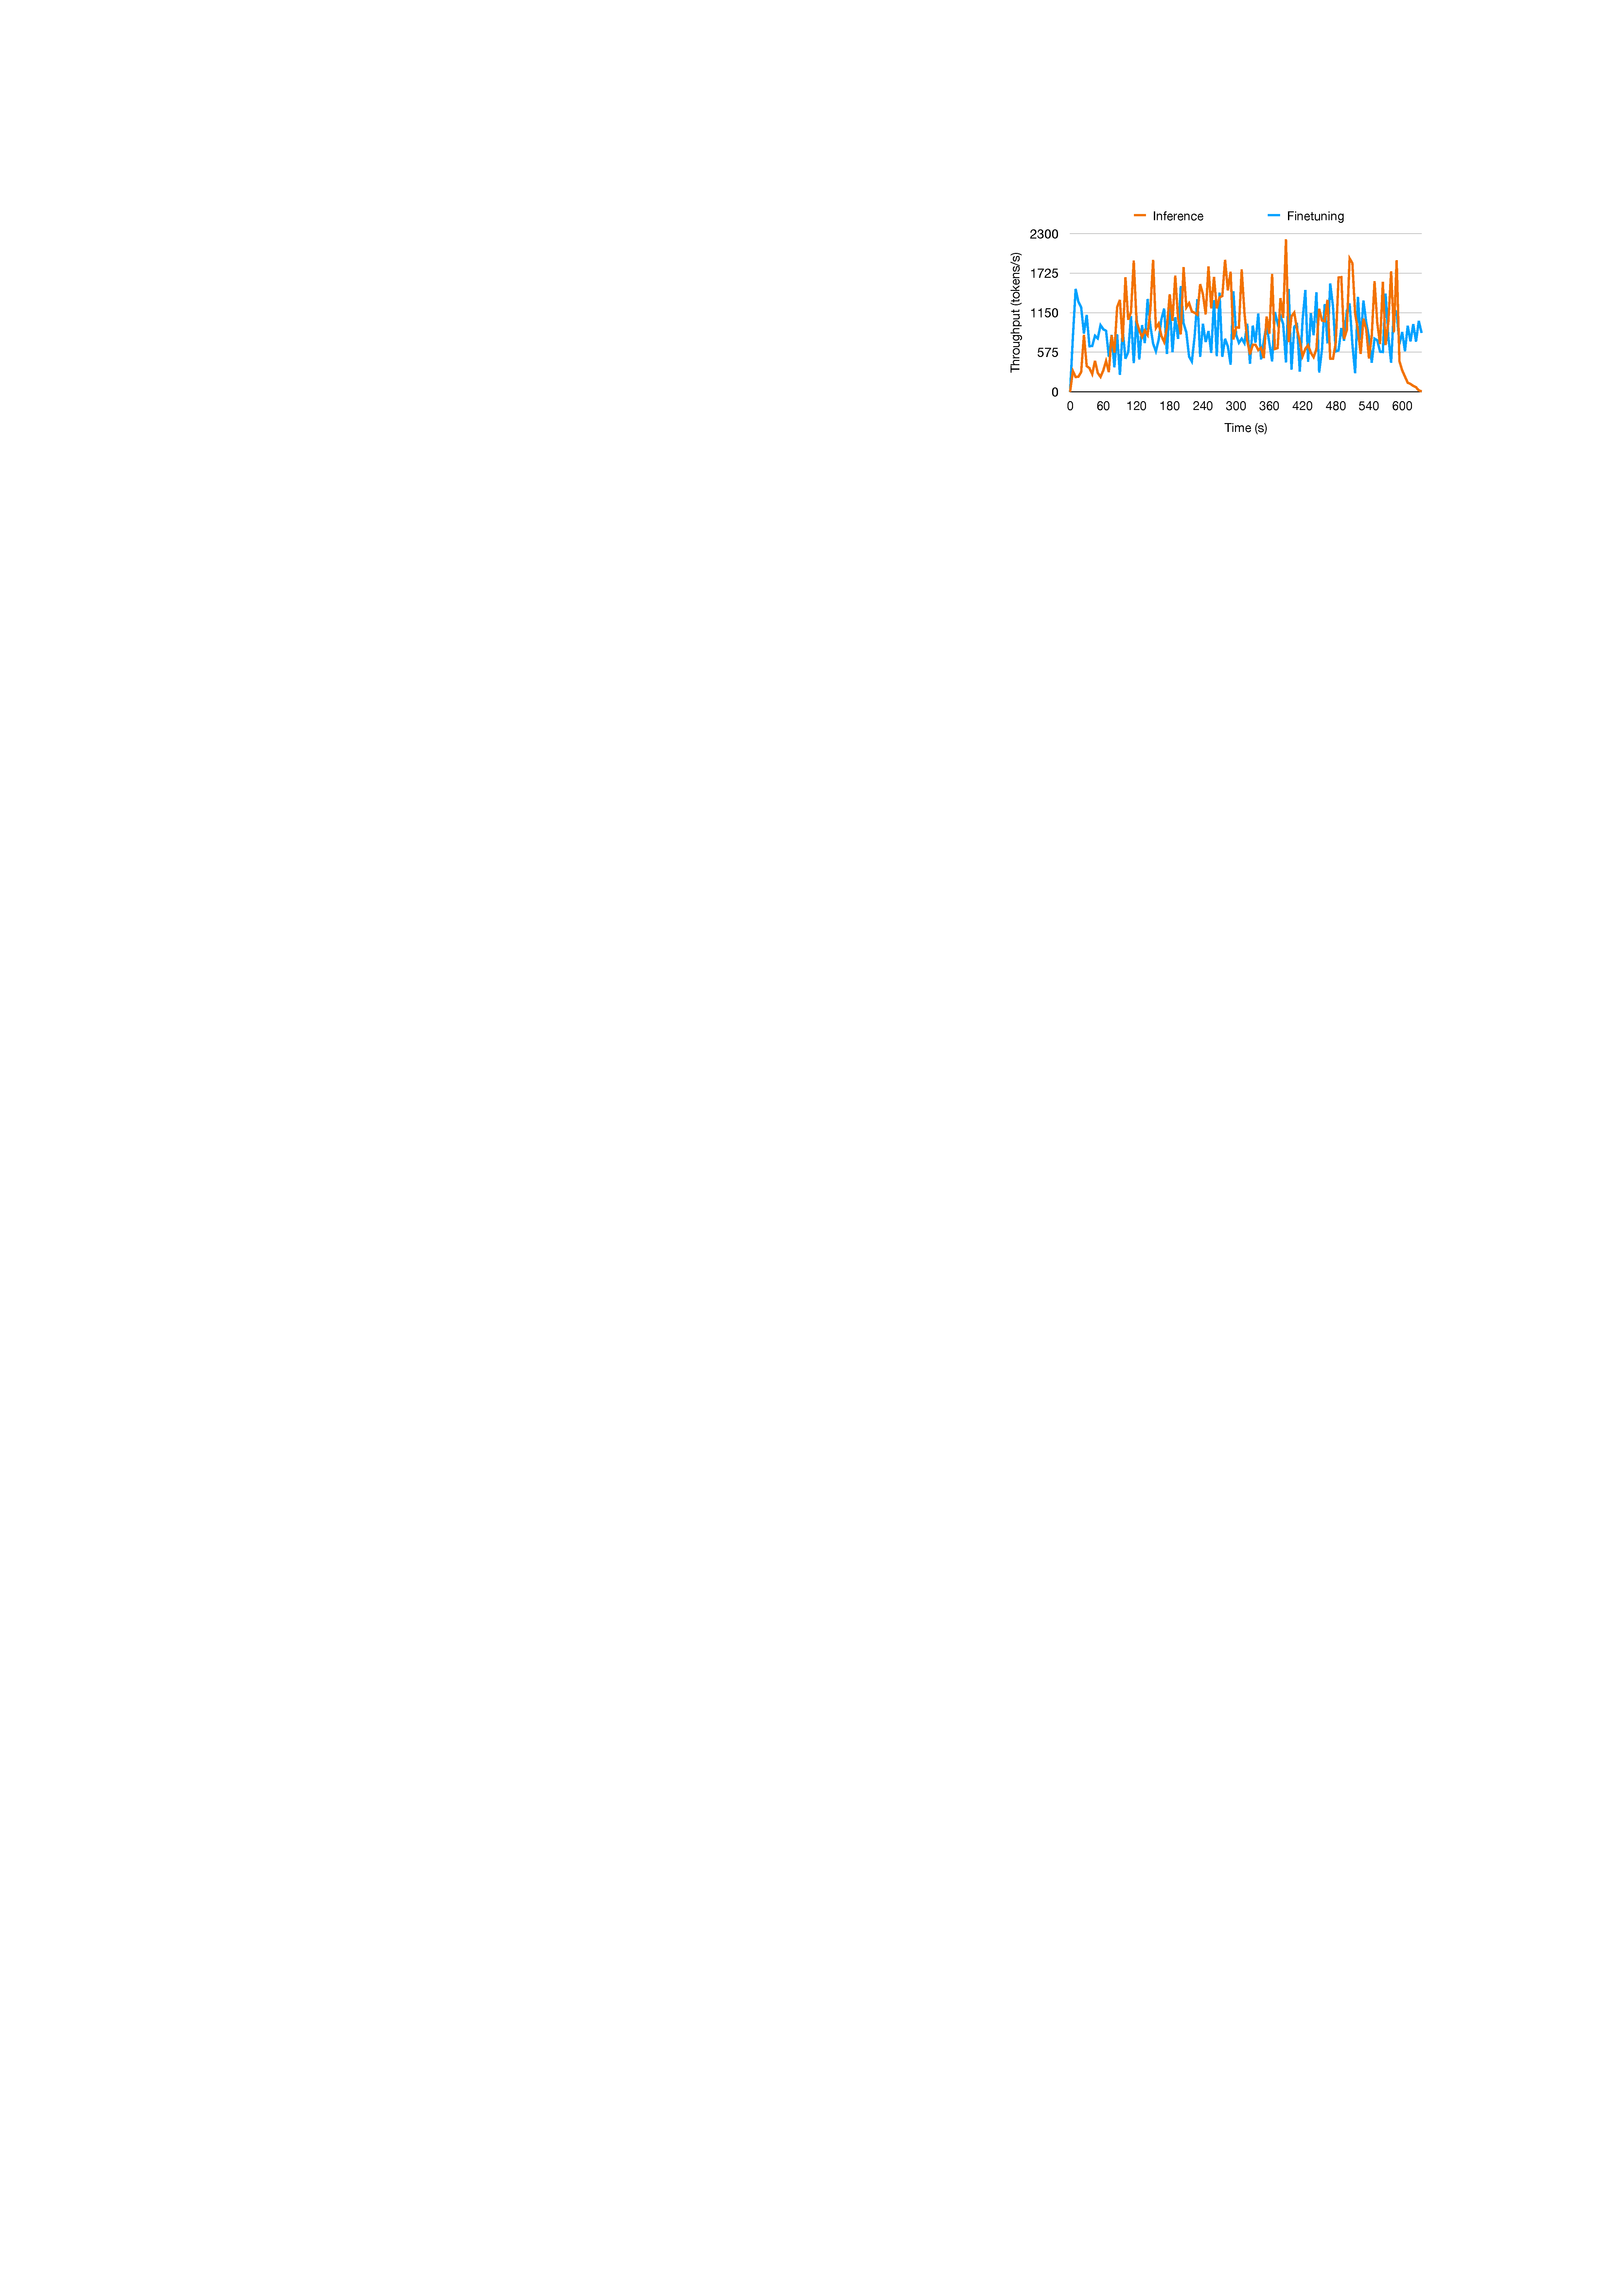
\includegraphics[width=\linewidth]{figures/flexllm/case_tpt.pdf}
      \caption{System throughput}
    \end{subfigure}
  \caption{Case study of \FlexLLM's system throughput for a fluctuating inference workload.}
  \label{flexllm:fig:case_study}
\end{figure}

\subsection{Case Study}
\label{flexllm:sec:exp:dynamic}
This case study demonstrates \FlexLLM's ability to dynamically adapt to fluctuating inference workloads in real time. We evaluate \FlexLLM using a 10-min interval of the BurstGPT trace with the Qwen-2.5-14B model. To ensure compatibility with our experiment environments, we replayed this trace segment and re-scaled its arrival intensity, as previous works have done~\cite{285173,258862,ali2022optimizing,miao2023spotserve}. In the experiment, each inference request and finetuning request are sampled from the ShareGPT dataset and the Sky-T1 dataset respectively.

In our case study, as shown in \Cref{flexllm:fig:case_study}, we observed that the arrival rate of the inference requests initially increased to a peak level after around 90 seconds, and then gradually decreased with some peaks. \FlexLLM could automatically detect the fluctuations in the workload and improve the ratio of inference tokens (vs.\ finetuning tokens) in each iteration's batch. This significantly increased inference throughput from a few hundred to 2.25K tokens/s.

\subsection{Memory Optimization}
\label{flexllm:eval:memory_optimization}
\begin{figure}[htbp]
    \centering
    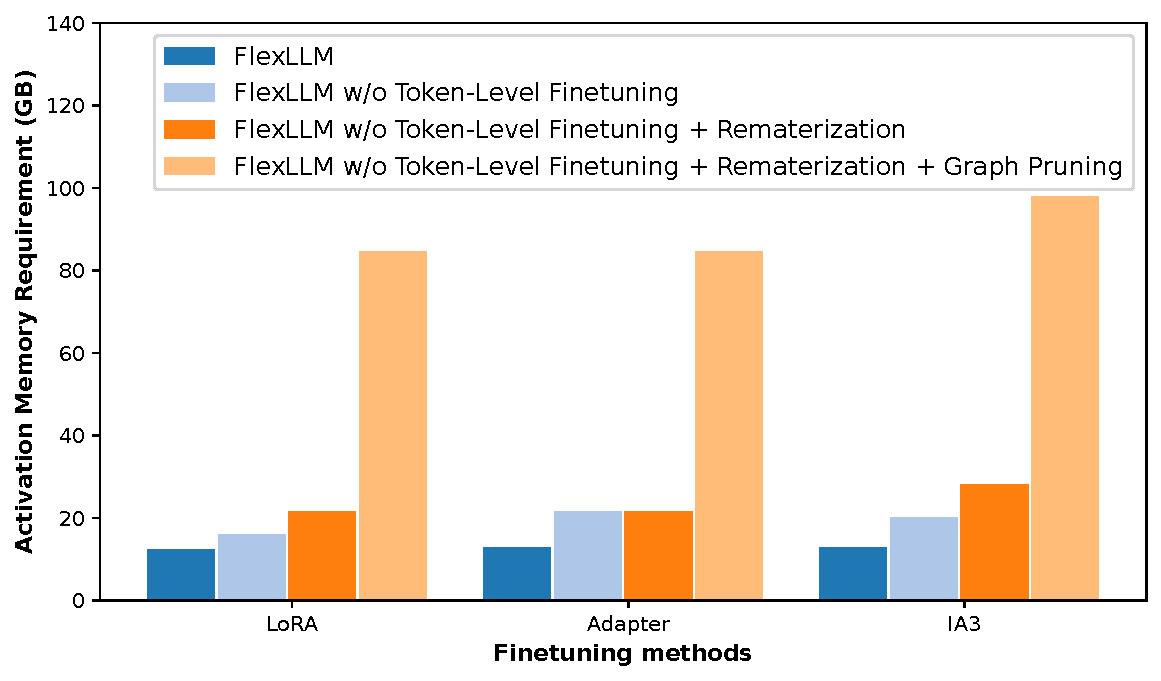
\includegraphics[width=0.7\linewidth]{figures/flexllm/fig_memory_act3.pdf}
    \caption{Ablation study of memory optimizations.}
    \label{flexllm:fig:memory_ablation}
\end{figure}

\FlexLLM introduces a series of memory optimizations to reduce the memory overhead of PEFT finetuning and allow co-serving finetuning with inference workloads.
%
To understand the effectiveness of \FlexLLM's memory optimizations, we perform an ablation study that incrementally turns off these optimizations (graph pruning, rematerialization, and token-level finetuning) and measures the memory requirements.
%
\Cref{flexllm:fig:memory_ablation} shows the activation memory requirements of \FlexLLM for different finetuning methods on a 70B LLM and a sequence length of 1024. \FlexLLM saves $85\%$--$87\%$ of the memory requirements for activations compared to existing approaches. The major improvement comes from graph pruning. With graph pruning only, \FlexLLM achieves a $71\%$--$74\%$ activation memory overhead reduction. Rematerialization and token-level finetuning further reduce memory overhead by $0$--$8\%$ and $4\%$--$10\%$, respectively. These memory optimizations are highly effective in practice, enabling \FlexLLM to retain sufficient memory for the inference requests' KV cache, ensuring eviction rates of 0\% in most cases and peaking at only 1.2\% for the largest model (Qwen2.5-32B) under the heaviest loads.

\paragraph{Eviction rates.}
\label{flexllm:sec:coserving_evictions}
\Cref{flexllm:tab:coserving_evictions} shows the percentage of inference requests experiencing a KV cache eviction during the evaluation of co-serving under the end-to-end experiment described in \Cref{flexllm:sec:exp:e2e}. Overall, the eviction rates are negligible. The eviction rate for the Qwen2.5-32B (TP=4) model is 0.29\% when the inference requests arrive at a rate of 16 req/s, and reaches a maximum of 1.20\% when the arrival rate is 20 req/s. In all other scenarios, no evictions occurred.

\begin{table}[htbp]
\centering
\caption{Percentage of inference requests experiencing a KV cache eviction under co-serving.}
\label{flexllm:tab:coserving_evictions}
\begin{tabular}{lccccc}
\toprule
Model & QPS=4 & QPS=8 & QPS=12 & QPS=16 & QPS=20 \\
\midrule
Llama-3.1-8B & 0.00\% & 0.00\% & 0.00\% & 0.00\% & 0.00\% \\
Qwen2.5-14B & 0.00\% & 0.00\% & 0.00\% & 0.00\% & 0.00\% \\
Qwen2.5-32B & 0.00\% & 0.00\% & 0.00\% & 0.29\% & 1.20\% \\
\bottomrule
\end{tabular}
\end{table}

\section{Discussion}
\label{flexllm:sec:discussion}

\subsection{Deployment Considerations}
\label{flexllm:sec:deployment}

\FlexLLM excels in scenarios where its co-serving architecture can maximize resource utilization while maintaining inference performance. \Cref{flexllm:tab:decision_framework} provides a decision framework to help practitioners identify when \FlexLLM delivers optimal benefits.

\FlexLLM is particularly well-suited for: (1) inference workloads with moderate burstiness and periods of low utilization, (2) environments with substantial and ongoing finetuning demands, and (3) deployments with moderate SLO requirements (50--100ms TPOT). These conditions allow \FlexLLM to fully exploit its co-serving capabilities and memory optimizations.

\begin{table}[htbp]
\centering
\caption{Decision framework for \FlexLLM adoption.}
\label{flexllm:tab:decision_framework}
\begin{tabular}{lcc}
\toprule
\textbf{Scenario} & \textbf{\FlexLLM} & \textbf{Separate Clusters} \\
\midrule
Bursty inference + high finetuning & \checkmark & \\
Consistent high inference load & & \checkmark \\
Minimal finetuning requirements & & \checkmark \\
Moderate SLOs (50--100ms TPOT) & \checkmark & \\
Strict SLOs ($<$25ms TPOT) & & \checkmark \\
Cost-sensitive deployments & \checkmark & \\
Operational simplicity priority & & \checkmark \\
\bottomrule
\end{tabular}
\end{table}

\FlexLLM's implementation comprises approximately 9K lines of code distributed across compilation, scheduling, memory management, and kernel integration components. The system leverages advanced techniques in GPU programming, distributed systems, and ML compiler optimizations to achieve its performance gains.

Under stricter SLO requirements, \FlexLLM's performance characteristics follow predictable queueing theory principles: co-serving introduces service time variance that can affect tail latencies. This trade-off between resource efficiency and latency guarantees becomes more pronounced as SLO targets approach inherent inference latency bounds, making \FlexLLM most effective in moderate SLO environments where it can fully utilize its resource optimization capabilities.

\subsection{Limitations and Future Work}
\label{flexllm:sec:limitations}
While \FlexLLM demonstrates significant improvements in GPU utilization and finetuning throughput, we identify several promising directions for future work. First, extending our implementation beyond offline finetuning scenarios where sequences are processed individually (batch size 1), to reinforcement-learning-based approaches like RLHF~\cite{sheng2024hybridflow,Stiennon2020} and Group Relative Policy Optimization (GRPO)~\cite{guo2025deepseek,MultiObjGRPO,DAPO} presents an exciting opportunity, as our token-level co-serving architecture naturally fits these methods where auto-regressive generation and gradient updates are tightly coupled. Second, developing adaptive strategies for workloads with consistently high inference demand could further expand co-serving opportunities. Finally, advancing beyond our current simple scheduling heuristics to more sophisticated algorithms that optimize for task priorities, deadlines, and QoS requirements could unlock additional system efficiency gains.

\section{Related Work}
\label{flexllm:sec:related}

\paragraph{ML serving and inference systems.} Numerous ML serving systems~\cite{258862,gunasekaran2022cocktail,lee2018pretzel,romero2021infaas,crankshaw2017clipper} address challenges like latency prediction, scalability, swapping~\cite{bai2020pipeswitch}, preemption~\cite{choi2020prema}, workload estimation~\cite{285173}, and cost-effectiveness~\cite{zhang2019mark}. Systems like Nexus~\cite{shen2019nexus} and Gpulet~\cite{choi2022serving} focus on batching and GPU virtualization for small models.
Recent LLM serving systems include vLLM~\cite{vllm}, Sarathi~\cite{agrawal2023sarathi}, SGLang~\cite{sglang}, AlpaServe~\cite{li2023alpaserve}, Punica~\cite{chen2023punica}, and S-LoRA~\cite{sheng2023s}, which improve throughput through batching and specialized PEFT kernels. Aqua~\cite{aqua2024} introduces fine-grained fair scheduling among multiple inference workloads.
Speculative decoding~\cite{chen2023accelerating,specinfer,suffixdecoding} can reduce serving latency and improve SLO attainment~\cite{adaserve} and goodput~\cite{turbospec}; combining it with co-serving is future work.

\paragraph{GPU resource sharing for ML.} GPU resource sharing focuses on efficient allocation among multiple ML users. Lyra~\cite{li2023lyra} allocates dedicated resources with dynamic adjustment. Gandiva~\cite{xiao2018gandiva} and Antman~\cite{xiao2020antman} use time-slicing for better cluster utilization. GSLICE~\cite{dhakal2020gslice} develops adaptive allocation schemes for different SLO constraints. Although these approaches cannot directly solve the resource utilization problem in PEFT service, we believe GPU resource sharing will be increasingly important as GPUs become more powerful.

\section{Summary}
\label{flexllm:sec:summary}
This chapter presented \FlexLLM, a system for co-serving parameter-efficient finetuning and inference of large language models on shared GPUs. We observed that finetuning and inference workloads have distinct GPU resource utilization characteristics---finetuning is throughput-oriented and latency-tolerant, whereas inference is bursty and latency-critical---and that running them on dedicated clusters wastes the capacity that must be reserved for inference bursts. \FlexLLM exploits the fact that both workloads share a frozen backbone LLM: its PEFT-as-a-Service interface unifies the two task types, static compilation (dependent parallelization and graph pruning) shrinks the memory footprint of finetuning by up to 80\%, and token-level finetuning combined with a hybrid token scheduler interleaves finetuning tokens with inference tokens at millisecond granularity while preserving inference SLOs.

Our evaluation on LLaMA-3.1-8B, Qwen-2.5-14B, and Qwen-2.5-32B shows that \FlexLLM matches the SLO attainment and inference throughput of a dedicated-cluster deployment while improving finetuning throughput by $1.9$--$4.8\times$ under heavy inference load and $2.5$--$6.8\times$ under light load, and that it outperforms temporal and spatial sharing baselines built on the same runtime. These results demonstrate that fine-grained, token-level co-serving is a practical way to reclaim the idle GPU capacity of LLM inference deployments without compromising their latency guarantees.

\chapter{\SuffixDecoding: Repetition-Aware Speculative Decoding for Agentic Workloads}
\label{ch:suffixdecoding}

% Chapter-local macros (prefixed to avoid collisions with other chapters).
\providecommand{\sdMaxSpec}{\texttt{MAX\_SPEC}\xspace}
\providecommand{\sdCount}{\texttt{COUNT}}
\providecommand{\sdChildren}{\texttt{CHILDREN}}
\providecommand{\sdParent}{\texttt{PARENT}}
\providecommand{\sdToken}{\texttt{TOKEN}}
\providecommand{\sdScore}{\texttt{SCORE}}

Speculative decoding is widely adopted to reduce latency in large language model (LLM) inference by leveraging smaller draft models capable of handling diverse user tasks. However, emerging AI applications, such as LLM-based agents, present unique workload characteristics: instead of diverse independent requests, agentic frameworks typically submit repetitive inference requests, such as multi-agent pipelines performing similar subtasks or self-refinement loops iteratively enhancing outputs. These workloads result in long and highly predictable sequences, which the speculative decoding methods discussed so far in this thesis, including \SpecInfer (\Cref{ch:specinfer}), do not effectively exploit. To address this gap, this chapter introduces \SuffixDecoding, a model-free speculative decoding method that utilizes efficient suffix trees to cache long token sequences from prompts and previous outputs. By adaptively speculating more tokens when acceptance likelihood is high and fewer when it is low, \SuffixDecoding effectively exploits opportunities for longer speculations while conserving computation when those opportunities are limited. Evaluations on agentic benchmarks, including SWE-Bench and Text-to-SQL, demonstrate that \SuffixDecoding achieves speedups of up to 5.3$\times$, outperforming state-of-the-art methods---2.8$\times$ faster than model-based approaches like EAGLE-2/3 and 1.9$\times$ faster than model-free approaches such as Token Recycling. \SuffixDecoding is open-sourced as part of ArcticInference at \url{https://github.com/snowflakedb/ArcticInference}.

\section{Introduction}
\label{suffixdecoding:sec:intro}

Large language models (LLMs) are foundational to agentic AI applications, such as automated coding assistants~\citep{openhands,yang2024sweagent}, multi-agent workflows~\citep{wang2024mixtureofagentsenhanceslargelanguage,chen2024autoagentsframeworkautomaticagent}, and retrieval systems~\citep{wang2024speculativeragenhancingretrieval,gao2024retrievalaugmentedgenerationlargelanguage}. Unlike basic chatbots, these workloads issue repetitive and predictable inference requests. For instance, multi-agent systems repeatedly perform similar tasks, and reasoning loops~\citep{wang2023selfconsistencyimproveschainthought,madaan2023selfrefine} regenerate similar token sequences. Despite this predictable repetition, existing methods fail to fully exploit recurring patterns, leaving latency as a bottleneck.

A popular strategy for mitigating inference latency is \emph{speculative decoding}~\citep{leviathan2022fast,chen2023accelerating,specinfer,cai2024medusasimplellminference,bita,draftverify}. While an LLM can only generate one token per forward pass, it can verify {\em multiple} tokens. Leveraging this phenomenon, speculative decoding methods use small ``draft'' models or additional decoding heads to predict multiple candidate tokens, which the LLM then verifies in parallel.

To efficiently handle the long repetitions common in agent-driven applications, speculative decoding methods must satisfy two critical requirements. First, they need to generate draft tokens rapidly and with minimal overhead, enabling maximal exploitation of long speculation lengths. Second, they must do so \emph{adaptively}---only generating more draft tokens when acceptance likelihood is high and fewer tokens when acceptance likelihood is low, to prevent verification from becoming a bottleneck.

However, existing speculative decoding approaches fall short in meeting these dual requirements. Model-based methods can use significant GPU time when speculating long sequences, and can incur memory contention and kernel-level transitions~\citep{sequoia,eagle2} that must be managed carefully. Conversely, existing model-free approaches, such as prompt-lookup decoding (PLD)~\citep{saxena2023prompt}, achieve low overhead and rapid token generation, but typically lack adaptivity. These methods speculate a fixed number of tokens irrespective of acceptance likelihood, leading to wasted computational resources on verifying long and improbable draft sequences.

\begin{figure}[htbp]
\centering
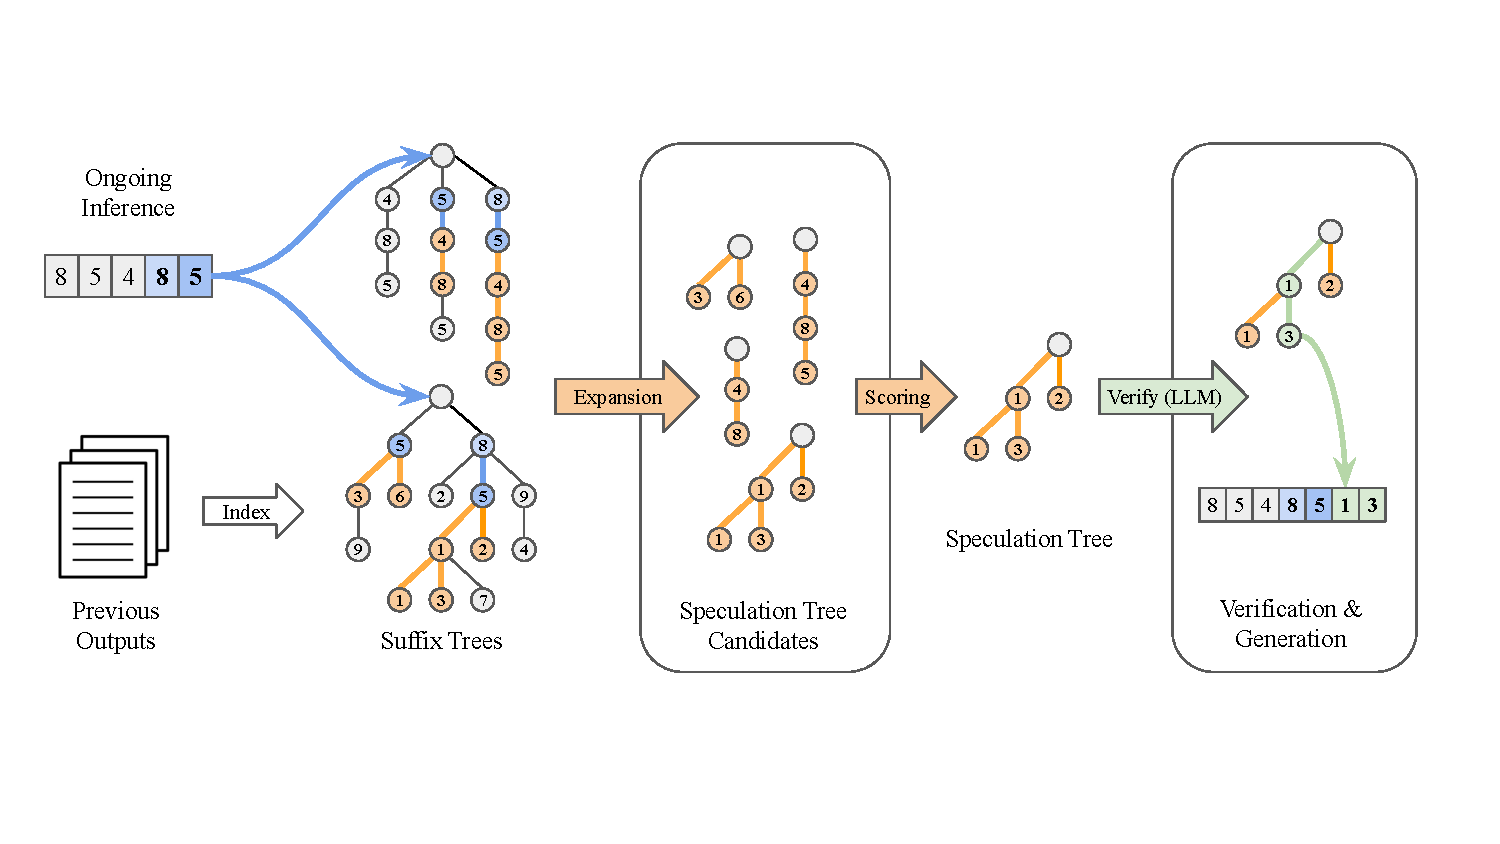
\includegraphics[width=\linewidth,trim={0 80 0 60},clip]{figures/suffixdecoding/suffix-decoding.pdf}
\caption{Overview of \SuffixDecoding's algorithm. Two suffix trees track ongoing inference (top-left) and previous outputs (bottom-left). \SuffixDecoding uses these trees to find matching patterns based on recently generated tokens. It constructs a speculation tree (middle) by selecting the most likely continuations, scoring them based on frequency statistics. Finally, the best candidate is verified by the LLM in a single forward pass (right), with accepted tokens (shown in green) being added to the output and used for the next round of speculation.}
\label{suffixdecoding:fig:suffix-decoding}
\end{figure}

To address these limitations, we introduce \SuffixDecoding (\Cref{suffixdecoding:fig:suffix-decoding}), a model-free speculative decoding method for repetitive, agent-driven workloads. \SuffixDecoding uses efficient suffix trees to cache long token sequences from prompts and previous outputs. Each node represents a token, and paths encode previously observed subsequences, enabling rapid pattern matching to identify continuations based on prior occurrences. Draft tokens are generated extremely quickly ($\sim$20 microseconds per token) without GPU overhead.

At each inference step, \SuffixDecoding adaptively limits its number of draft tokens based on the length of the pattern match, and uses frequency-based statistics captured within the suffix trees to score and select the best speculation candidate. Longer pattern matches enable confident speculation of longer token sequences, maximizing its effectiveness on agentic workloads, while shorter pattern matches trigger conservative speculation to avoid computational waste. Moreover, \SuffixDecoding can seamlessly integrate with existing model-based speculative decoding methods. This flexibility enables a hybrid approach that leverages suffix-tree-based speculation for repetitive, predictable agentic workloads, while exploiting the strengths of model-based speculation methods for open-ended conversational tasks, thus achieving the best of both worlds.

We evaluate \SuffixDecoding on two practical agent-driven workloads: SWE-Bench, an LLM-based software engineering benchmark, and AgenticSQL, a proprietary multi-agent pipeline application for SQL generation. We compare with state-of-the-art model-based and model-free speculative decoding methods using Spec-Bench~\citep{xia2024unlockingefficiencylargelanguage}, showing up to 2.8$\times$ faster decoding than EAGLE-2/3~\citep{li2025eagle3scalinginferenceacceleration}, and 1.9$\times$ faster decoding than Token Recycling~\citep{luo2024turningtrashtreasureaccelerating}. For SWE-Bench, we also measured the comprehensive, end-to-end task completion time---including prompt prefilling, token generation, and execution of external actions---and demonstrate speculative speedups of up to 4.5$\times$. These results highlight that \SuffixDecoding substantially reduces latency for real-world agentic applications, addressing a critical bottleneck in practical inference scenarios.

The rest of this chapter is organized as follows. Background on LLM inference, speculative decoding, and agentic workloads is covered in \Cref{ch:background}. \Cref{suffixdecoding:sec:method} presents the design of \SuffixDecoding, and \Cref{suffixdecoding:sec:evaluation} evaluates it against state-of-the-art baselines, including end-to-end experiments in vLLM, ablation studies, scalability measurements, and detailed per-task results. \Cref{suffixdecoding:sec:discussion} discusses limitations and extensions, \Cref{suffixdecoding:sec:related} surveys related work, and \Cref{suffixdecoding:sec:summary} concludes the chapter.

\section{\SuffixDecoding}
\label{suffixdecoding:sec:method}

The goal of \SuffixDecoding is to enable fast, adaptive speculative decoding over long sequences, particularly suited for agentic applications where repeated inference calls often contain highly predictable and overlapping token sequences. In such settings, long stretches of output can be accurately predicted from prior and ongoing requests.

To fully exploit these opportunities, \SuffixDecoding must address two key challenges. First, it must support \emph{fast generation of speculative sequences}---including long continuations---without relying on draft models or expensive token-by-token prediction. Second, it must be \emph{adaptive} to the current prediction context: aggressively speculating long continuations only when they are likely to be accepted, and speculating shorter sequences when uncertain to avoid wasted verification compute.

To support fast speculation, \SuffixDecoding builds a \emph{suffix tree}~\citep{10.1109/SWAT.1973.13} over the tokens in the current and prior requests, and uses the suffix tree to generate speculative tokens.
The root node of the tree represents the beginning of a suffix of any token sequence stored in the tree, each child of a node represents a specific token which is a possible continuation from that node, and the path from the root to each node represents a distinct subsequence.

For each request, we consider speculating token sequences from (1) the prompt and output of that request, and (2) the outputs of prior requests. Doing so captures the source of output token repetition from many agentic algorithms, including self-consistency, self-refinement, and multi-agent pipelines.

\SuffixDecoding leverages suffix trees to perform fast pattern matching and find possible continuations of token sequences. Suppose the prompt and output tokens of an ongoing inference is \( x_{1:t} \). Consider a suffix \( x_{t-p+1:t} \) of length \( p \), which we will refer to as the \emph{pattern} sequence. We walk the suffix tree starting from the root node, and at each step taking the child that corresponds to token \( x_{t-p+i} \). If no such child exists, then the pattern is not found and \SuffixDecoding reverts to standard non-speculative decoding. Otherwise, after \( p \) steps, we arrive at a node whose descending paths are the possible continuations of the pattern sequence.

Although this procedure can quickly find a (potentially large) set of candidate sequences, verifying all of them in speculative decoding may be cost-prohibitive. Instead, \SuffixDecoding builds a much smaller and more likely speculation tree through a greedy expansion and scoring procedure, and uses this smaller tree in tree-based speculation. An overall illustration of \SuffixDecoding is shown in \Cref{suffixdecoding:fig:suffix-decoding}, which we detail in the rest of this section.

\subsection{Suffix Tree Construction}
\label{suffixdecoding:sec:construction}

Building the suffix tree and updating it as part of an online inference service involves two stages. First, the previous inference outputs can be added to the tree in a single offline processing step (e.g., from historical logs), or online during inference serving after each inference request completes. Second, the current ongoing prompt and output tokens are added online as new requests are received and as each new token is generated.

In practice, we found it convenient to maintain two different suffix trees: a \emph{global} tree for the previously generated outputs, and a separate \emph{per-request} tree for the current ongoing inference request. This circumvents the complexities and overheads due to synchronizing the suffix tree updates from multiple concurrent requests. The global tree can be constructed offline in \( O(n) \) time, while the per-request tree can be efficiently constructed and updated online~\citep{10.1007/BF01206331}.

Although suffix trees are memory-efficient at \( O(n) \) space, the global tree can still become large when there are many previous outputs. However, they only require CPU memory, which is typically plentiful and under-utilized in LLM serving scenarios. For example, AWS \texttt{p5.48xlarge} instances are often used for LLM serving and have 2TB of main memory, which is easily enough to support a suffix tree over millions of historical outputs and billions of tokens. Given typical server configurations, \SuffixDecoding can cache approximately a month's worth of generated tokens before requiring cache eviction (see \Cref{suffixdecoding:sec:scalability} for a detailed memory overhead analysis).

\subsection{Speculation Tree Expansion}
\label{suffixdecoding:sec:expansion}

Given a pattern sequence \( x_{t-p+1:t} \) of an ongoing inference \( x_{1:t} \), \SuffixDecoding can quickly find a node \( N_p \) in the global or per-request suffix tree whose descending paths are the possible continuations of the pattern sequence. To select a smaller, more likely sub-tree that is of a more practical size for speculative verification, we start with the single node \( N_p \) and grow a sub-tree greedily by expanding one leaf node at a time.

In particular, we define:
\[
C(N) = \frac{\sdCount(N)}{\sum_{M \in \sdChildren(\sdParent(N))} \sdCount(M)}
\]
\[
D(N) = \begin{cases}
    D(\sdParent(N)) \times C(N), & \text{if $N \neq N_p$}\\
    1, & \text{otherwise}
\end{cases},
\]
where \( \sdCount(N) \) is the number of occurrences of node \( N \) in the reference corpus, which can be computed when constructing the suffix tree. Starting with the single node \( N_p \) in our speculation sub-tree, we consider all children of all of its leaf nodes, and add the node \( N \) with the highest \( D(N) \). This process is repeated until the sub-tree reaches a predetermined size limit, \sdMaxSpec.

Intuitively, \( C(N) \) estimates the probability that \( \sdToken(N) \) would be the next observed token in a subsequence \( \sdToken(N_p), \ldots, \sdToken(\sdParent(N))\), and \( D(N) \) estimates the probability that \( \sdToken(N) \) would be ultimately accepted by the speculative tree verification, assuming the output tokens follow historical patterns.
Thus, \SuffixDecoding builds the speculation tree by greedily adding leaf nodes that it believes to be the most likely to be accepted during verification.

\begin{algorithm}[htbp]
\caption{Speculation tree generation in \SuffixDecoding.}
\label{suffixdecoding:alg:suffix-decoding}
\begin{algorithmic}[1]
\Function{ExpandSpeculationTree}{$N_p$, \sdMaxSpec}
   \State \textbf{Input:} suffix tree node $N_p$, size limit \sdMaxSpec
   \State Initialize $T \gets \{ N_p \}$
   \While{$|T| < \text{\sdMaxSpec}$}
   \State $N \gets \arg\max_{N \in \sdChildren(\text{LEAVES}(T))} D(N)$
   \State $T \gets T \cup \{ N \}$
   \EndWhile
   \State \textbf{return} $T$
\EndFunction
\Statex
\Function{MatchPattern}{$S$, $x_{1:t}$, $p$}
   \State \textbf{Input:} suffix tree $S$, sequence $x_{1:t}$, pattern length $p$
   \State Initialize $N_p \gets \text{ROOT}(S)$
   \For{$i=1$ \textbf{to} $p$}
   \If{$\text{NO\_CHILD}(N_p, x_{t-p+i})$}
   \State \textbf{return} $\emptyset$
   \EndIf
   \State $N_p \gets \text{CHILD}(N_p, x_{t-p+i})$
   \EndFor
   \State \textbf{return} $N_p$
\EndFunction
\Statex
\Function{GenerateCandidateTree}{$S_g$, $S_r$, $x_{1:t}$, $\alpha$, $P$}
   \State \textbf{Input:} global suffix tree $S_g$, per-request suffix tree $S_r$, sequence $x_{1:t}$, max speculation factor $\alpha$, max pattern size $P$
   \State Initialize $T_{\text{best}} \gets \emptyset$, $\sdScore_{\text{best}} \gets 0$
   \For{$S$ \textbf{in} $\{S_g, S_r\}$}
   \For{$p=1$ \textbf{to} $P$}
   \State $N \gets \textsc{MatchPattern}(S, x_{1:t}, p)$
   \State $T \gets \textsc{ExpandSpeculationTree}(N, \alpha p)$
   \If{$\sdScore(T) > \sdScore_{\text{best}}$}
   \State $T_{\text{best}} \gets T$
   \State $\sdScore_{\text{best}} \gets \sdScore(T)$
   \EndIf
   \EndFor
   \EndFor
   \State \textbf{return} $T_{\text{best}}$
\EndFunction
\end{algorithmic}
\end{algorithm}

\begin{figure}[htbp]
\centering
\begin{subfigure}[t]{0.42\linewidth}
\centering
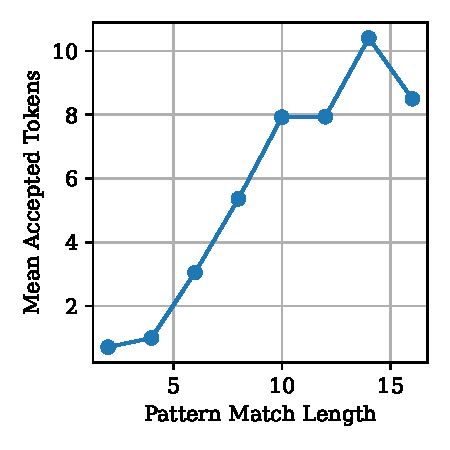
\includegraphics[width=\linewidth,trim={5 5 5 5},clip]{figures/suffixdecoding/pattern_vs_accept.pdf}
\caption{Average accepted tokens vs.\ pattern match length.}
\label{suffixdecoding:fig:pattern-vs-accept}
\end{subfigure}
\hspace{0.04\linewidth}
\begin{subfigure}[t]{0.42\linewidth}
\centering
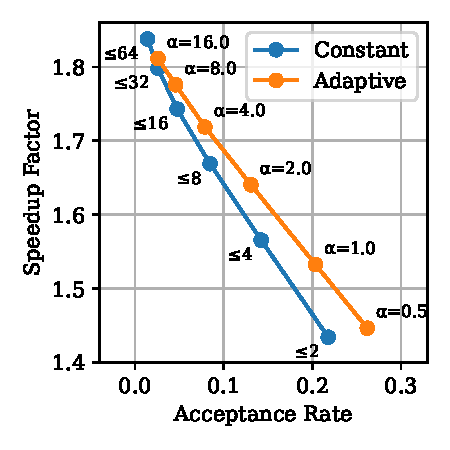
\includegraphics[width=\linewidth,trim={5 5 5 5},clip]{figures/suffixdecoding/max_spec_tokens_vs_factor.pdf}
\caption{Constant vs.\ adaptive \sdMaxSpec.}
\label{suffixdecoding:fig:constant-vs-adaptive}
\end{subfigure}
\caption{Motivation for adaptive speculation lengths. (a) The mean number of accepted tokens increases with the length of the pattern match, which motivates \( \sdMaxSpec = \alpha p \). (b) This choice achieves a better trade-off between acceptance rate and speculative speedup than a constant \sdMaxSpec.}
\label{suffixdecoding:fig:adaptive-motivation}
\end{figure}

\subsection{Adaptive Speculation Lengths}
\label{suffixdecoding:sec:adaptive}

While the procedure above allows \SuffixDecoding to cache and quickly speculate long token sequences based on empirical probability estimates, it also needs a mechanism for \emph{adaptively} controlling the number of tokens it speculates. \SuffixDecoding achieves this by dynamically adjusting \sdMaxSpec. Low values mean fewer but more likely tokens would be chosen for speculation, while higher values mean more but less likely tokens would be chosen. If too low, then the speedup from speculation can be limited, and if too high, then compute may be wasted on verifying unlikely tokens.

To guide how to adaptively set \sdMaxSpec, we observed that the number of accepted tokens in practice typically increases with longer pattern sequence lengths \( p \) (\Cref{suffixdecoding:fig:pattern-vs-accept}). Thus, we define \sdMaxSpec adaptively as
\[
\sdMaxSpec(p) = \alpha p,
\]
where \( \alpha \) is a user-defined max speculation factor. \Cref{suffixdecoding:fig:constant-vs-adaptive} shows that setting \sdMaxSpec adaptively according to the pattern length results in a better trade-off between acceptance rate and speculative speedup. In practice, we found that \( \alpha \in [1, 4] \) works well for agentic applications.

\subsection{Speculation Tree Scoring}
\label{suffixdecoding:sec:scoring}

So far, we have discussed how to obtain a speculation tree given a suffix tree and a pattern length \( p \). However, \SuffixDecoding maintains two suffix trees, the global suffix tree and the per-request suffix tree, each with many choices for \( p \). To obtain just a single speculation tree, we build speculation trees for both the global suffix tree and the per-request suffix tree, and for a range of values of \( p \). Then, a single speculation tree is selected according to a scoring function:
\[
\sdScore(T_{spec}) = \sum_{N \in T_{spec}} D(N).
\]
Intuitively, if \( D(N) \) estimates the probability that node \( N \) in a speculation tree \( T_{spec} \) would be accepted, then \( \sdScore(T_{spec}) \) estimates the expected number of accepted tokens. \SuffixDecoding then selects the \( T_{spec} \) with the highest \( \sdScore \) as the final speculation tree to be verified.
The end-to-end candidate generation from speculation tree expansion to scoring is described in \Cref{suffixdecoding:alg:suffix-decoding}.

\subsection{Hybrid Suffix Speculative Decoding}
\label{suffixdecoding:sec:hybrid}

Lastly, we find that \( \sdScore(T_{spec}) \) can be used to dynamically decide between using \SuffixDecoding or falling back to a model-based speculation method, which is useful for practical scenarios when the workload can be mixed between agentic and more diverse applications. Specifically, for each decoding iteration, we always speculate using \SuffixDecoding first. If \( \sdScore(T_{spec}) > \tau \), where \( \tau \) is a configurable threshold, then \SuffixDecoding's draft tokens are used. Otherwise, we use a fall-back speculation method, such as EAGLE-3~\citep{li2025eagle3scalinginferenceacceleration}.

As a practical guideline, we find that setting $\tau$ close to the mean accepted tokens of the fallback speculator works well for mixed workloads, while using \SuffixDecoding alone ($\tau = 0$) is optimal for highly repetitive agentic tasks. A detailed sensitivity analysis of $\tau$ across different workload types is provided in \Cref{suffixdecoding:sec:threshold-sensitivity}. For batched serving scenarios, \SuffixDecoding can be integrated with existing batch-level speculation control methods (see \Cref{suffixdecoding:sec:batch-speculation}).

\section{Evaluation}
\label{suffixdecoding:sec:evaluation}

\subsection{Evaluation Methodology}
\label{suffixdecoding:sec:evaluation-methodology}

\begin{figure}[htbp]
\centering
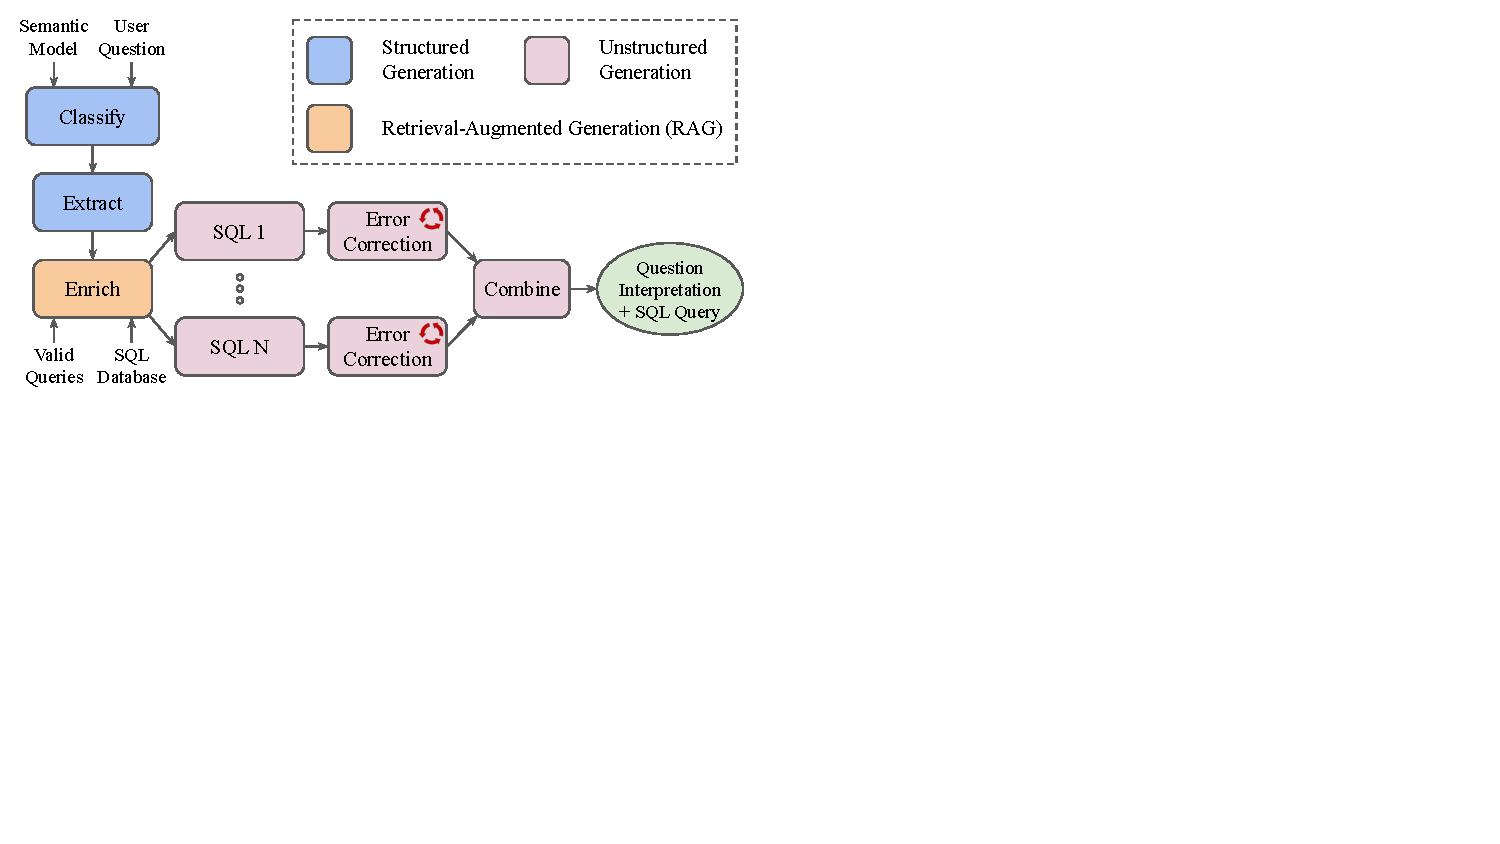
\includegraphics[width=0.75\linewidth,trim={0 220 360 0},clip]{figures/suffixdecoding/agentic-sql.pdf}
\caption{AgenticSQL is a multi-agent workflow consisting of structured generation, unstructured generation, and retrieval-augmented generation steps across several different LLMs. Useful features are extracted from the user question (Classify and Extract) and supplemented with retrieved context (Enrich). Several text-to-SQL steps propose solutions to the user question (SQL 1\ldots N) in parallel with feedback from an error corrector. A last Combine step synthesizes the proposed SQL candidates into a final SQL query and text response.}
\label{suffixdecoding:fig:agentic-sql}
\end{figure}

\paragraph{Baseline Comparisons.}
We compare with both model-based and model-free speculative decoding methods using Spec-Bench~\citep{xia2024unlockingefficiencylargelanguage}: (1) \emph{EAGLE-2} and \emph{EAGLE-3}~\citep{li2025eagle3scalinginferenceacceleration}, state-of-the-art model-based speculators, (2) \emph{Prompt-Lookup Decoding (PLD)}~\citep{saxena2023prompt}, a simple model-free speculator based on n-gram matching, and (3) \emph{Token Recycling}~\citep{luo2024turningtrashtreasureaccelerating}, a more recent model-free speculator that sources token sequences from both the prompt and previous outputs. EAGLE-3 and Token Recycling both leverage tree speculation~\citep{specinfer}.

\paragraph{Datasets and Agentic Applications.}
We evaluate on both agentic and non-agentic workloads. For agentic applications, we trace requests from two real applications: OpenHands~\citep{openhands} on \emph{SWE-Bench}~\citep{jimenez2024swebenchlanguagemodelsresolve} (a GitHub issue resolution benchmark), and \emph{AgenticSQL}, a proprietary multi-agent SQL generation workflow (\Cref{suffixdecoding:fig:agentic-sql}). For non-agentic workloads, we use Spec-Bench, consisting of open-ended, single-turn tasks across 13 categories, including 8 MT-Bench categories (Writing, Roleplay, Reasoning, Math, Coding, Extraction, STEM, Humanities). We include Spec-Bench to stress-test \SuffixDecoding's limitations and evaluate the hybrid fallback mechanism.

\paragraph{End-to-end System Evaluation.} We implemented \SuffixDecoding in vLLM~\citep{vllm}. By running OpenHands live, we show \SuffixDecoding accelerates end-to-end task completion times, including prefill and code execution.

\paragraph{Hardware Configuration.}
We conducted our experiments on a single \texttt{p5.48xlarge} AWS instance equipped with \( 8\times \) NVIDIA H100 80GB GPUs and 2TB of main memory.

\paragraph{Setup of the Spec-Bench Experiments.}
We conducted our Spec-Bench experiments (\Cref{suffixdecoding:sec:baseline-comparisons}) by running the Spec-Bench codebase from the original repository with the following modifications. First, we updated the code to work with the latest version of the \texttt{transformers} library, which is required to run recent open-source LLMs such as \texttt{meta-llama/Llama-3.1}. We also added support for arbitrary datasets (such as SWE-Bench and AgenticSQL) and implemented \SuffixDecoding within the framework. We ran each baseline using one GPU and a batch size of 1, just like in the original Spec-Bench code.

\paragraph{Setup of the vLLM SWE-Bench Experiment.}
For the end-to-end SWE-Bench experiment (\Cref{suffixdecoding:sec:vllm-swebench-results}), we served the \texttt{all-hands/openhands-lm-32b-v0.1-ep3} model locally using vLLM, with a tensor parallelism degree of 4 and with prefix caching enabled. We used the FlashInfer kernels for sampling. We made some minor modifications to vLLM to record the per-request and per-step statistics of interest (time-per-token latency, throughput, acceptance length, acceptance rate). We used the same settings for all baselines. We ran the OpenHands daemon on the same machine, and used the OpenAI API to interact with the vLLM server. We ran OpenHands with the CodeActAgent~\citep{wang2024executablecodeactionselicit} with \texttt{ITERATIVE\_EVAL\_MODE=true}, and a maximum of 100 iterations, as recommended by the OpenHands authors. We used a maximum of 16 concurrent workers to run the SWE-Bench tasks.

\paragraph{Simulated Ablations.}
In addition to our main evaluation using real hardware, we also leverage a simulated verifier for the ablation experiments in \Cref{suffixdecoding:sec:ablation-experiments}. Given a prompt \( x_{1:n} \) and example ground-truth response \( y_{n+1:t} \), we can accurately simulate speculative verification for greedy sampling by verifying that speculated token \( x_{n+i} = y_{n+i} \).

\subsection{Baseline Comparisons}
\label{suffixdecoding:sec:baseline-comparisons}

\begin{figure}[htbp]
\centering
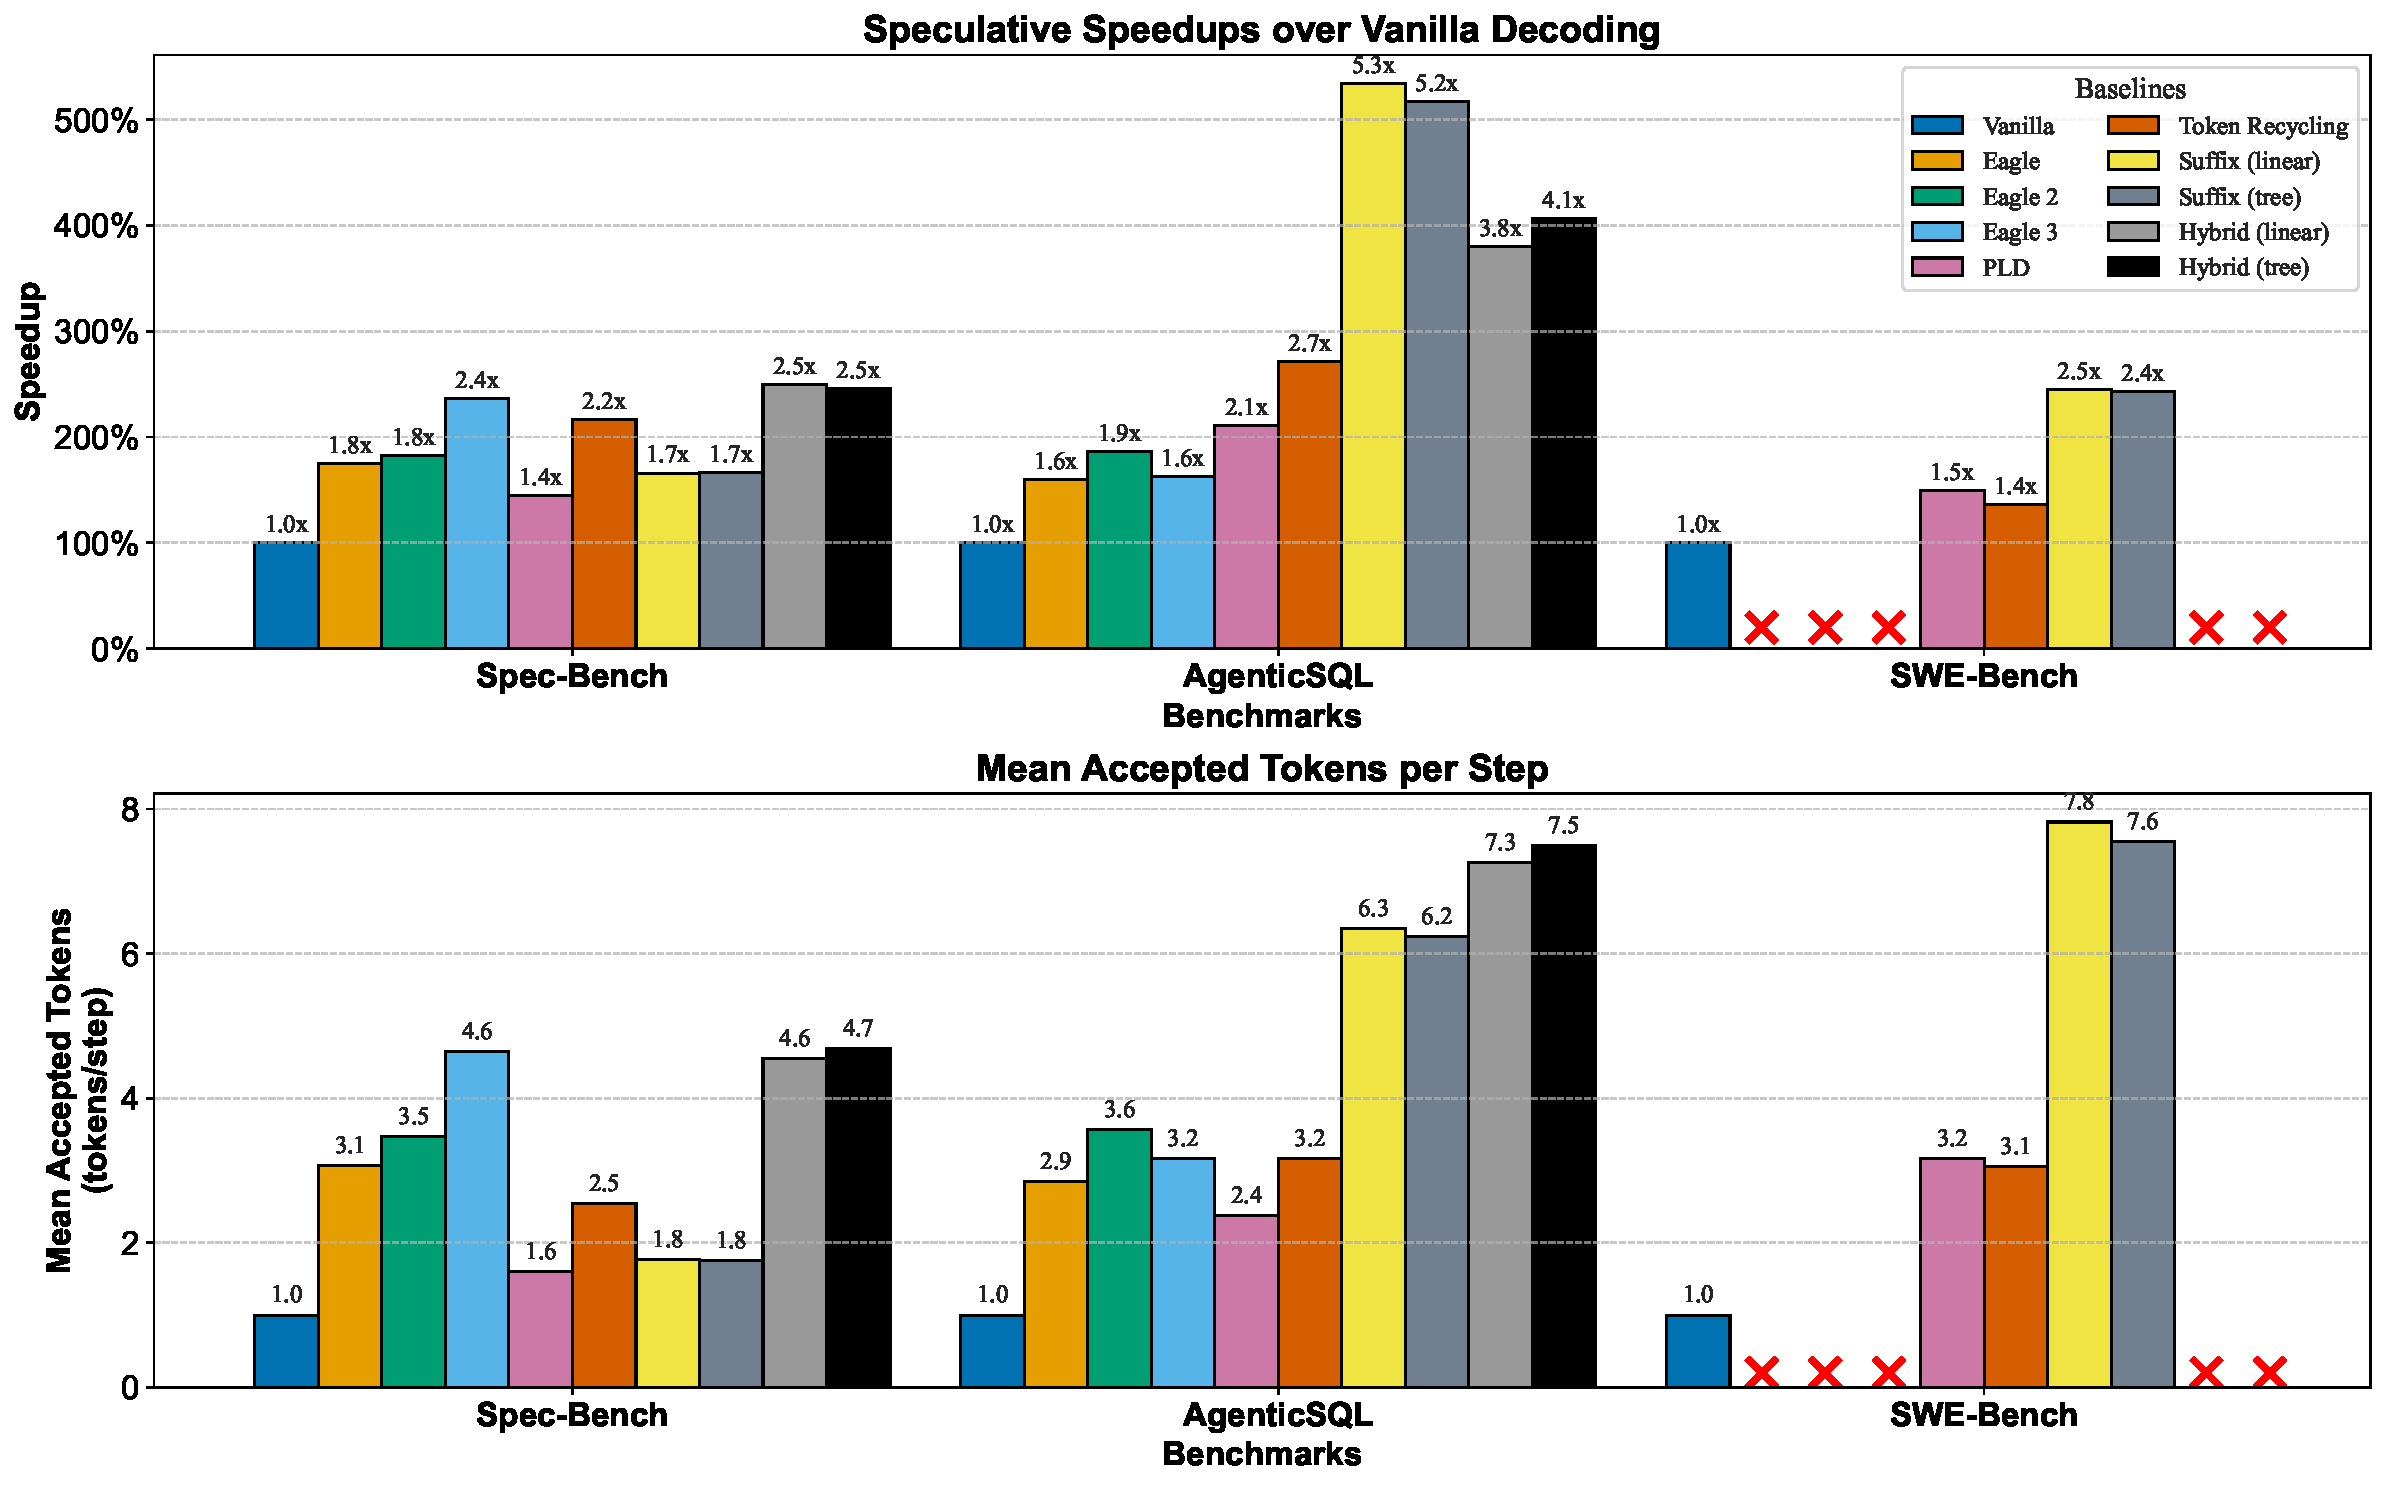
\includegraphics[width=\linewidth]{figures/suffixdecoding/benchmark_comparison.pdf}
\caption{Speculative speedups (top) and mean accepted tokens per step (bottom) compared to vanilla decoding for \SuffixDecoding and baseline methods on three benchmarks: Spec-Bench, AgenticSQL, and SWE-Bench. Experiments use Llama-3.1-8B-Instruct on a single H100 GPU with batch size 1. Speedup is measured as the ratio of wall-clock time-per-output-token relative to vanilla decoding. Suffix (tree) and Hybrid (tree) use \SuffixDecoding's tree speculation algorithm, which constructs a speculation tree from the suffix tree for parallel verification. Suffix (linear) and Hybrid (linear) use a simpler linear speculation approach that only allows sequential token chains. The hybrid variants combine \SuffixDecoding with EAGLE-3, dynamically selecting between suffix-based and model-based speculation based on pattern match confidence. Note that EAGLE-2/3 and Token Recycling failed to run on several SWE-Bench tasks due to long context lengths ($>$8192 tokens), indicated by missing bars. Spec-Bench represents a non-agentic workload and is included for comparison. Further sub-task breakdowns, including the raw time-per-output-token and mean acceptance lengths, can be found in \Cref{suffixdecoding:sec:detailed-results}.}
\label{suffixdecoding:fig:throughput-tpot}
\end{figure}

We compare \SuffixDecoding with EAGLE-2, EAGLE-3, PLD, and Token Recycling on SWE-Bench and AgenticSQL. We also run the Spec-Bench standard dataset, which is a more traditional non-agentic workload. \Cref{suffixdecoding:fig:throughput-tpot} shows the results. First, on the agentic workloads, \SuffixDecoding outperforms all baselines. In AgenticSQL, \SuffixDecoding obtains a mean speedup of $5.3\times$ over vanilla decoding, a $2.8 \times$ improvement over EAGLE-2/3, and $1.9\times$ higher than Token Recycling. In SWE-Bench, EAGLE-2/3 fail due to their maximum sequence length limitations. \SuffixDecoding obtains a mean speedup of $2.5\times$ over vanilla decoding, a $1.7 \times$ improvement over PLD, the next best baseline. \SuffixDecoding's superior performance in agentic workloads can be attributed to its consistently higher mean accepted tokens per decoding step. In AgenticSQL, \SuffixDecoding reaches 6.3 mean accepted tokens per step---substantially higher than EAGLE-3 (3.6 tokens) and Token Recycling (3.2 tokens). In SWE-Bench, \SuffixDecoding achieves 7.8 mean accepted tokens per step, while PLD only accepts 3.2 tokens per step on average.

On non-agentic workloads such as Spec-Bench (which includes open-ended single-turn tasks and 8 MT-Bench categories), \SuffixDecoding alone is outperformed by EAGLE-2/3 and Token Recycling, as expected for less repetitive scenarios. However, the hybrid approach of \SuffixDecoding + EAGLE-3 achieves the best of both worlds: we speculate with the faster \SuffixDecoding method whenever possible and fall back to EAGLE-3 when the speculation score is too low. The hybrid approach obtains a mean speedup of $2.5\times$ over vanilla decoding, outperforming the $2.4\times$ speedup from standalone EAGLE-3 and the $2.2\times$ speedup from Token Recycling.

The hybrid approach also performs well in AgenticSQL, achieving a $4.1\times$ speedup in the tree variant, significantly better than the $1.9\times$ speedup from standalone EAGLE-2/3 and the $2.7\times$ speedup from Token Recycling. These speedups are achieved thanks to the hybrid approach's impressive 7.5 mean accepted tokens per step, more than $2\times$ higher than EAGLE-2/3 and Token Recycling. \SuffixDecoding has a slightly lower mean acceptance length of 6.3, but its much lower speculation cost and higher acceptance rate make it the winning solution in agentic tasks ($5.3\times$ average speedup compared to the $4.1\times$ speedup of the hybrid approach).

\paragraph{A Peek into a Speculation Tree.}

\begin{figure}[htbp]
    \centering
    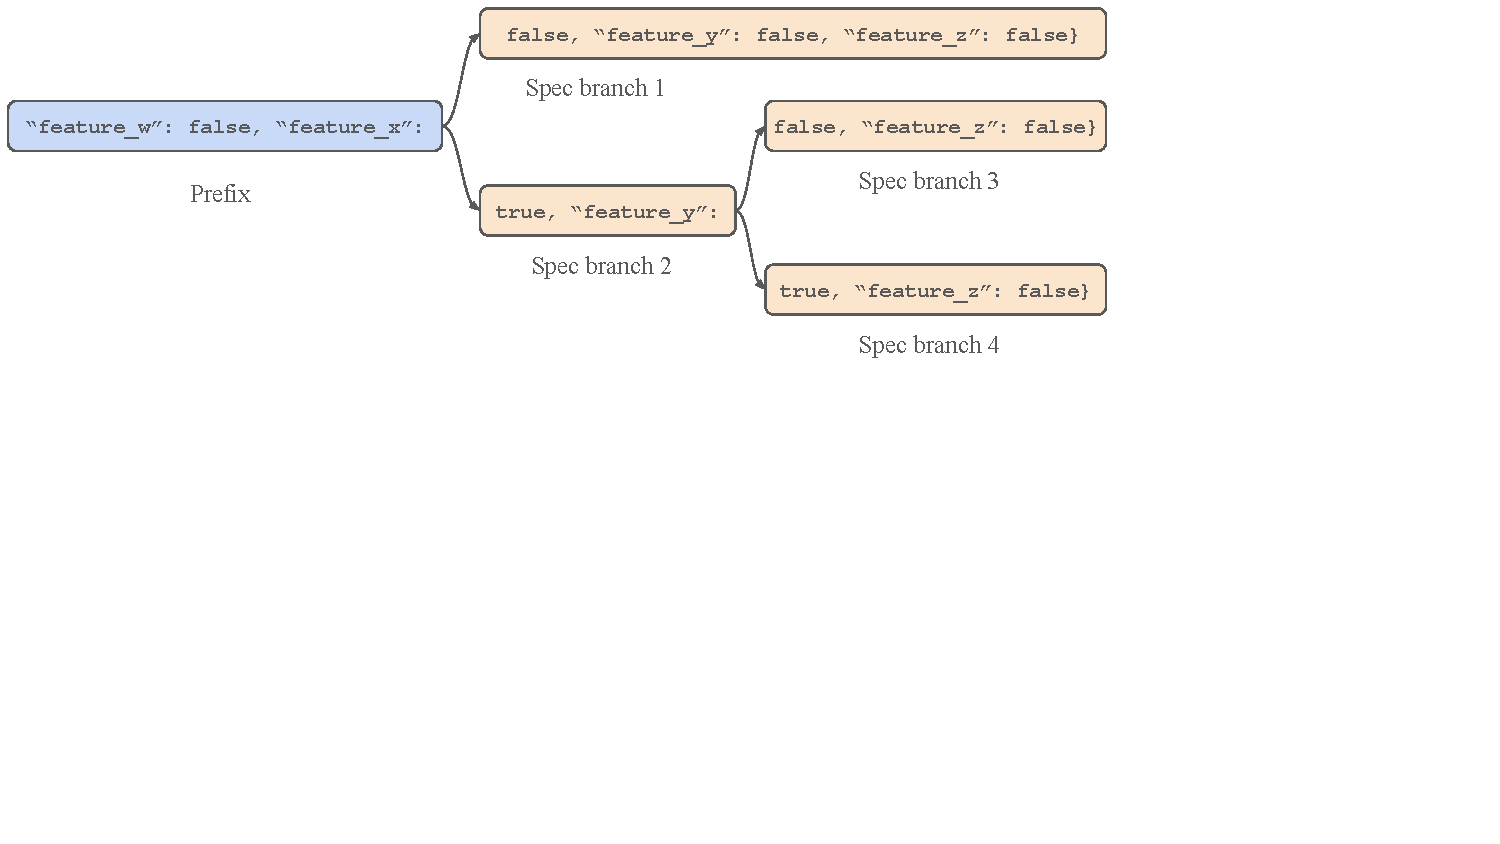
\includegraphics[width=\linewidth,trim={0 230 180 0},clip]{figures/suffixdecoding/speculation-tree-example.pdf}
    \caption{A \SuffixDecoding speculation tree containing 66 tokens for the AgenticSQL Extract task.}
    \label{suffixdecoding:fig:speculation-tree-example}
\end{figure}

To gain some intuition into why \SuffixDecoding performs so well for certain tasks, we examine how it builds a speculation tree for the AgenticSQL Extract task.
The outputs of the Extract task have many characteristics in common. First, they are all JSON documents following the same format and key names, with keys often appearing in the same order. Second, many of the features are discrete values, and in particular, boolean true/false values. These patterns are recorded in \SuffixDecoding's global suffix tree and guide its speculation tree construction.

\Cref{suffixdecoding:fig:speculation-tree-example} shows an example of a speculation tree constructed by \SuffixDecoding. We observed many instances of large speculation trees that branch at each boolean true/false value of several consecutive features. These speculation trees always contain a branch with high acceptance, advancing output generation by dozens of tokens or more in one step.
Although this is one specific example of a speculation tree, it demonstrates that \SuffixDecoding can find complex patterns in previous outputs, particularly for structured generation tasks, that help accelerate output generation.

\subsection{End-to-End SWE-Bench on vLLM}
\label{suffixdecoding:sec:vllm-swebench-results}

In this section, we show that \SuffixDecoding can be efficiently integrated into vLLM, a popular inference system used in production deployments, and that it can effectively accelerate end-to-end agentic task completion time. For this experiment, we run OpenHands directly on vLLM with \SuffixDecoding, so the agent is solving each benchmark problem live. We also use the specially-trained LLM \texttt{all-hands/openhands-lm-32b-v0.1-ep3}, which was fine-tuned for SWE-Bench and achieves 37.2\% on SWE-Bench Verified. Since there are no model-based methods with draft models trained for this LLM, we compare with vLLM's native implementation of PLD.

\Cref{suffixdecoding:fig:vllm-spec-bench} shows the results. First, we note that decoding time (i.e., output generation) takes a majority of the time across all SWE-Bench tasks, dominating both prefilling and agentic actions (i.e., code execution). In this end-to-end scenario, \SuffixDecoding outperforms PLD by 1.3--3\(\times\), leading to a 1.8--4.5\(\times\) speculative speedup over vanilla decoding. Since \SuffixDecoding exactly preserves the output distribution of the LLM, it matches the original model's 37.2\% score on SWE-Bench Verified.

\begin{figure}[htbp]
\centering
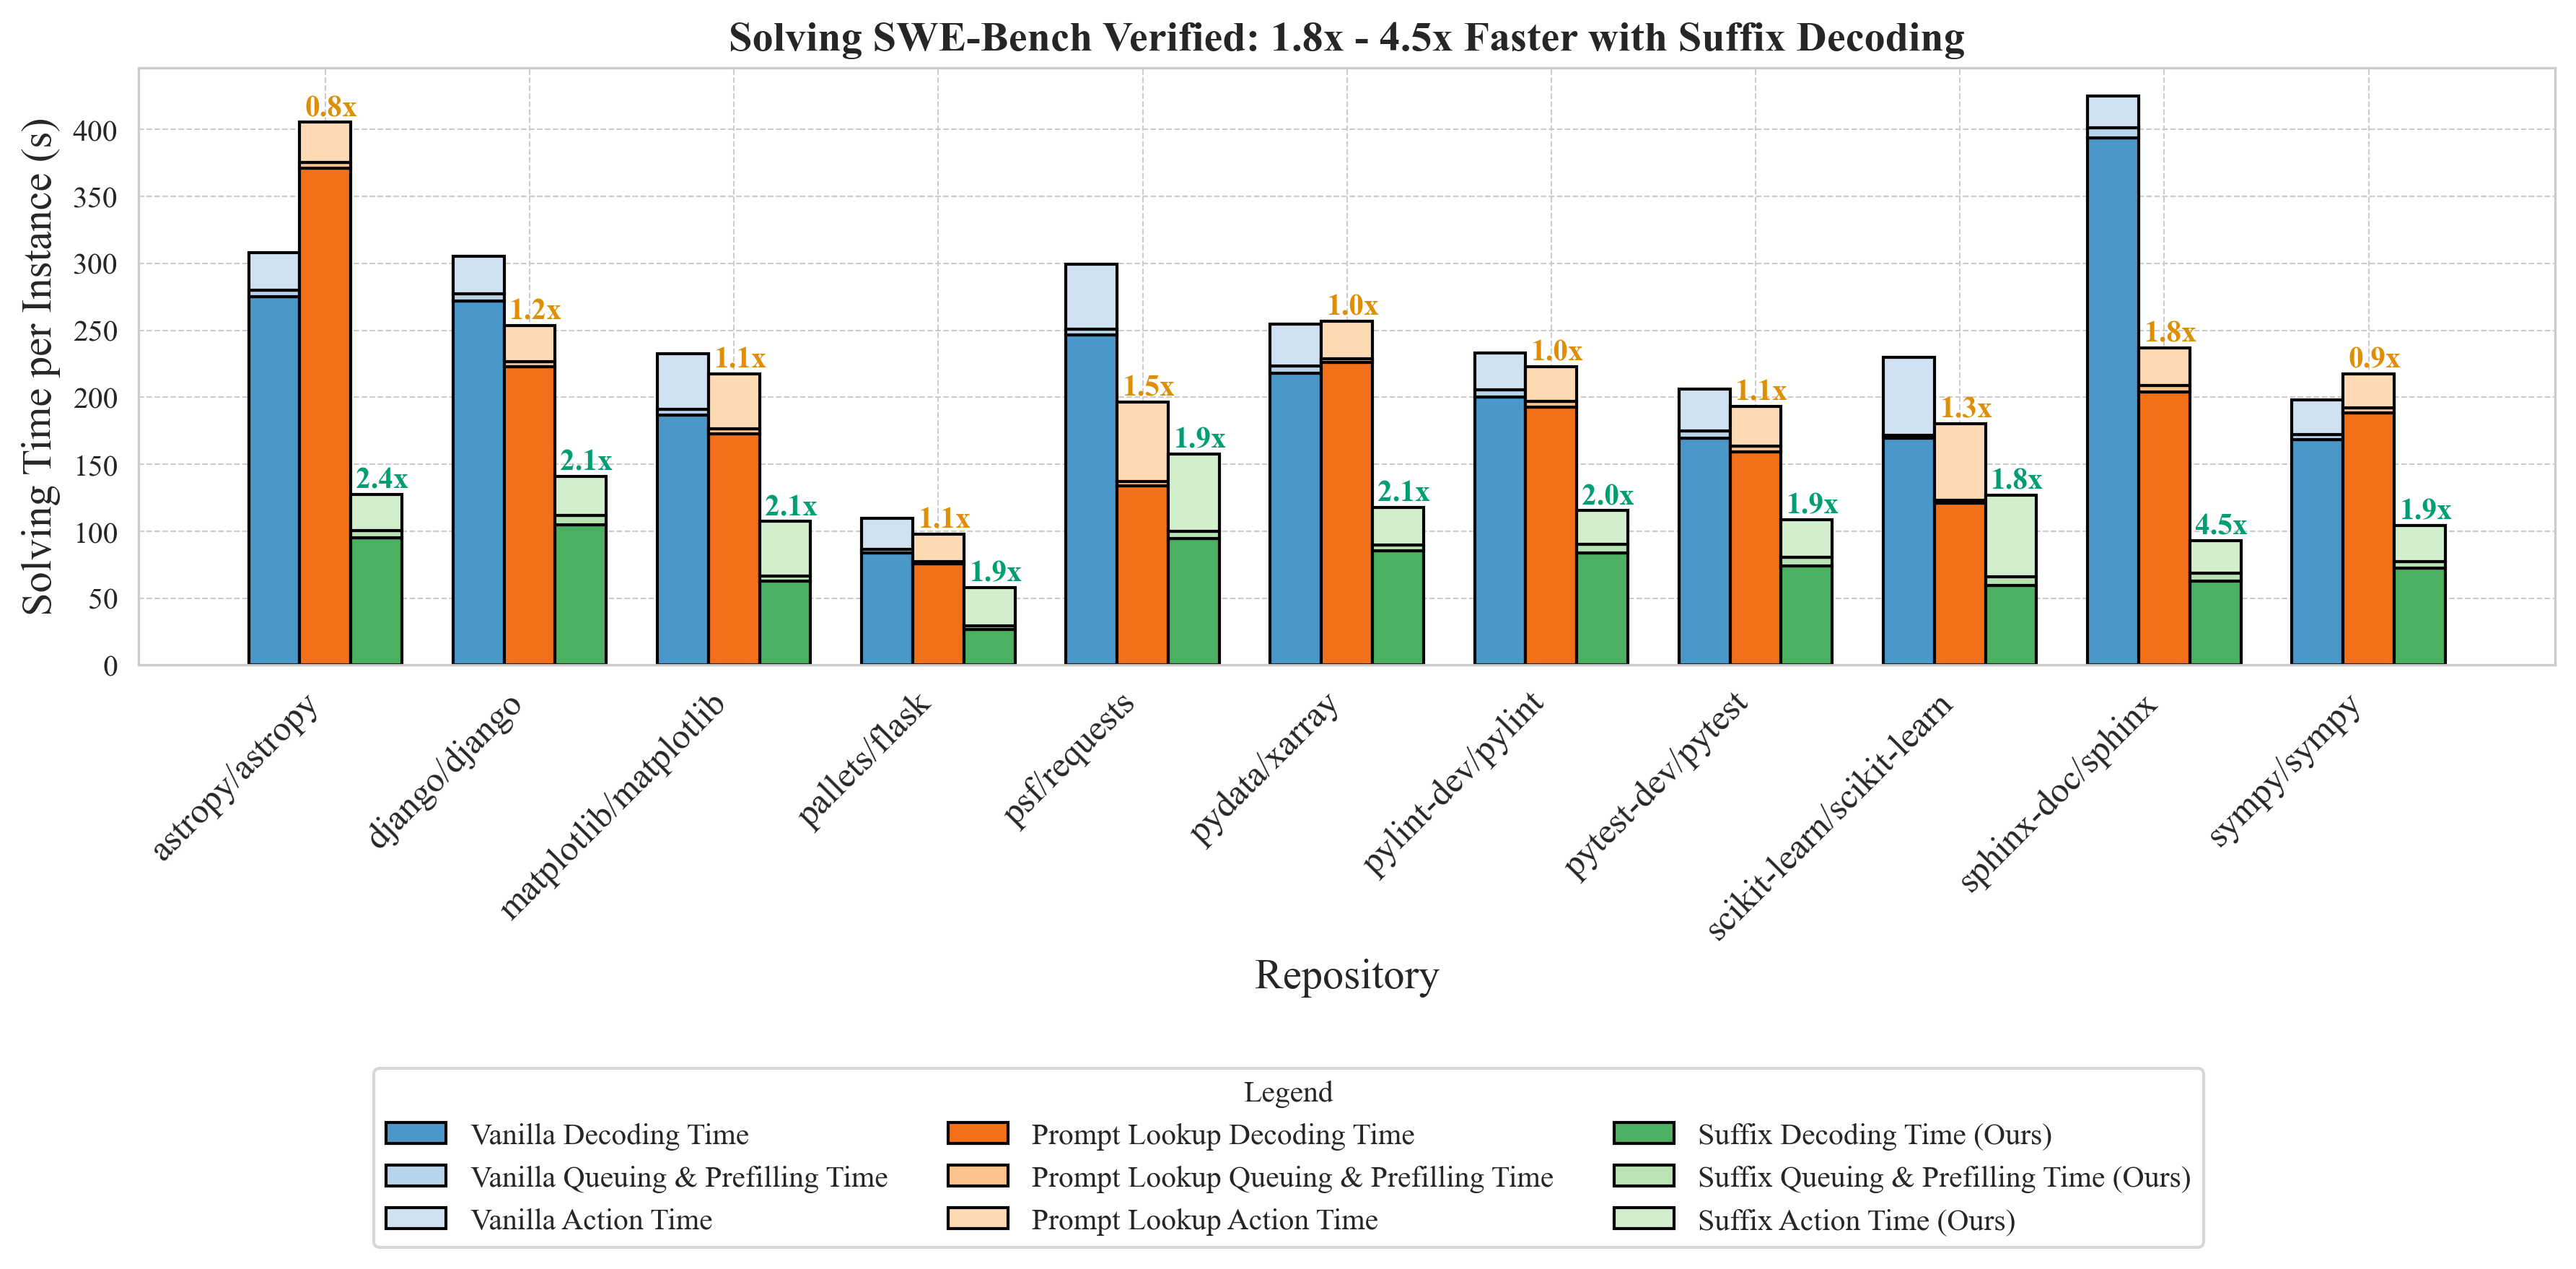
\includegraphics[width=\linewidth]{figures/suffixdecoding/combined_latency_breakdown.png}
\caption{End-to-end task-completion time of the OpenHands agent on SWE-Bench Verified. The benchmarks are run with a concurrency of 8 tasks running simultaneously. vLLM is deployed on 4 H100 GPUs configured with 4-way tensor parallelism and prefix caching enabled. The results are broken down by the different code repositories in SWE-Bench.}
\label{suffixdecoding:fig:vllm-spec-bench}
\end{figure}

\subsection{Ablation Experiments}
\label{suffixdecoding:sec:ablation-experiments}

In this section, we present ablation studies on \SuffixDecoding using a simulated verifier on offline traces. Given a ground-truth prompt-response pair from an LLM, we can verify the draft tokens proposed by \SuffixDecoding by comparing with the ground truth responses. Besides the AgenticSQL traces, some of these studies use the following additional datasets.

\begin{enumerate}
\item \emph{WildChat}~\citep{zhao2024wildchat}. We use instructions from the WildChat dataset, which consists of real-world interactions between users and the ChatGPT service. WildChat represents the most diverse and open-domain dataset used in our evaluations.
\item \emph{Magicoder}~\citep{wei2023magicoder}. Specifically, we use instructions from the Magicoder-Evol-Instruct-110K dataset, which consists of code-related questions and instructions generated via Self-Instruct~\citep{codealpaca,wang-etal-2023-self-instruct} and further augmented for difficulty and diversity~\citep{luo2023wizardcoder} by GPT-4.
\item \emph{SpiderSQL}. Spider~\citep{yu-etal-2018-spider} is a dataset of manually-annotated questions and SQL responses over 200 different databases with multiple tables, covering 138 different domains. We use instructions from DAIL-SQL~\citep{10.14778/3641204.3641221}, which consists of LLM prompts with instructions to answer questions from Spider using structured SQL code.
\end{enumerate}

\paragraph{Global vs.\ Per-Request Suffix Trees.}

\begin{figure}[htbp]
    \centering
    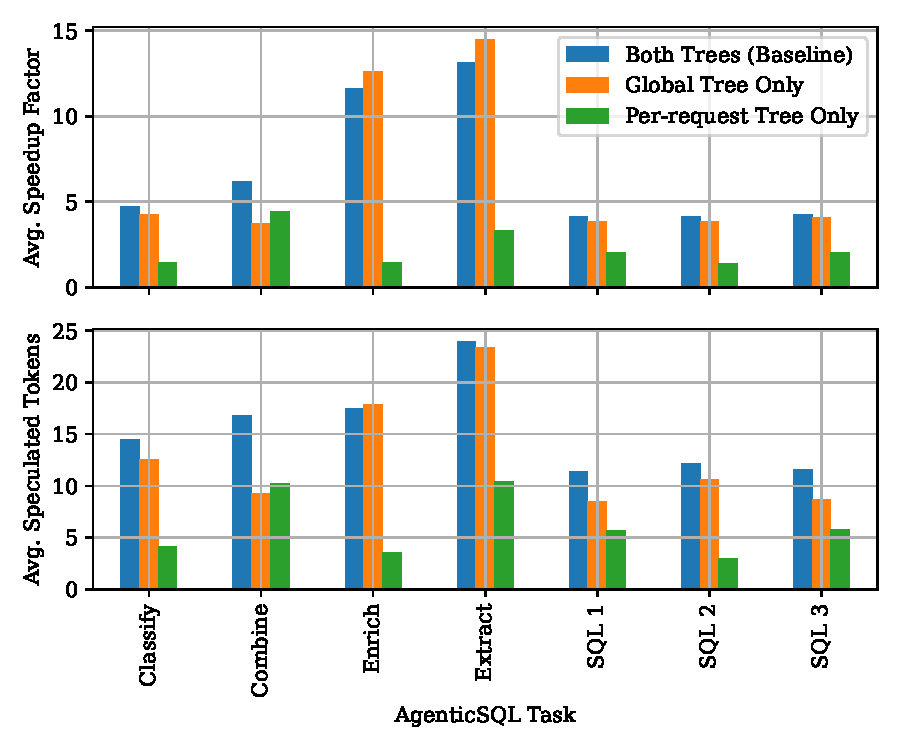
\includegraphics[width=0.7\linewidth]{figures/suffixdecoding/per_request_tree.pdf}
    \caption{Speedup factor and number of speculated tokens for the tasks in AgenticSQL. \SuffixDecoding was run with only the global suffix tree, only the per-request suffix tree, and both (baseline).}
    \label{suffixdecoding:fig:per-request-tree}
\end{figure}

We study the impact of the two suffix trees: the global suffix tree containing previous outputs, and the per-request suffix tree containing the prompt and generation of the current ongoing request. To do so, we ran the tasks in AgenticSQL using \SuffixDecoding (1) with the global suffix tree only, (2) with the per-request suffix tree only, and (3) using both trees.

\Cref{suffixdecoding:fig:per-request-tree} shows the results. First, we note that with the exception of the Content Enrichment (Enrich) and Extract steps, using both suffix trees performs better than using just one. The small degradations on the Enrich and Extract steps suggest that, when both trees are present, \SuffixDecoding may sometimes choose a speculation tree from the per-request suffix tree when the global suffix tree may have been the better choice. Improvements to \SuffixDecoding's speculation tree scoring mechanism may help bridge this gap.

Second, the global tree outperforms the per-request tree on all tasks except for Combine. This is because the Combine task heavily re-uses tokens from its context, which are the proposed SQL solutions from the previous steps in the workflow. Although there is a diversity of task characteristics, \SuffixDecoding is able to achieve high speedups on all of them by combining both suffix trees.

\paragraph{\SuffixDecoding in Open-Ended Scenarios.}

\begin{figure}[htbp]
\centering
\begin{subfigure}[t]{0.42\linewidth}
\centering
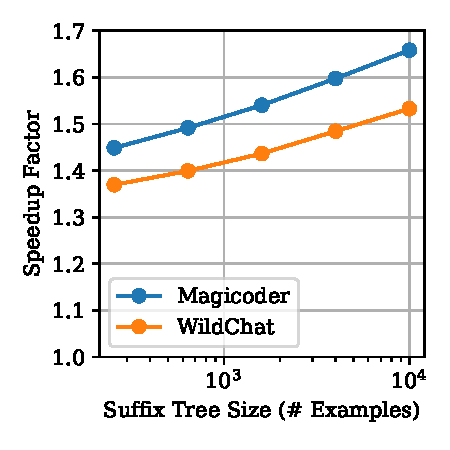
\includegraphics[width=\linewidth,trim={5 5 5 5},clip]{figures/suffixdecoding/global_suffix_tree_size_speedup.pdf}
\caption{Speedup.}
\label{suffixdecoding:fig:global-suffix-tree-size-speedup}
\end{subfigure}
\hspace{0.04\linewidth}
\begin{subfigure}[t]{0.42\linewidth}
\centering
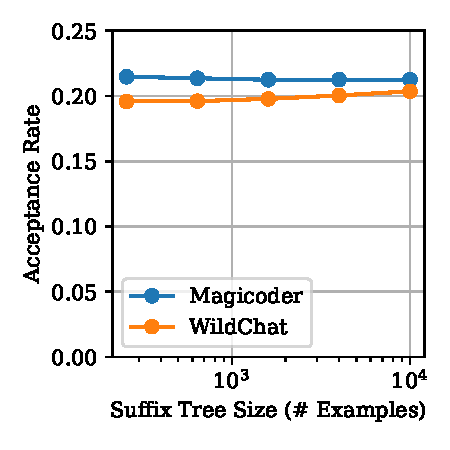
\includegraphics[width=\linewidth,trim={5 5 5 5},clip]{figures/suffixdecoding/global_suffix_tree_size_acceptance.pdf}
\caption{Acceptance rate.}
\label{suffixdecoding:fig:global-suffix-tree-size-acceptance}
\end{subfigure}
\caption{Speedup (left) and acceptance rate (right) vs.\ global suffix tree size for Magicoder and WildChat (\( \alpha = 1 \)). The speedup from \SuffixDecoding continues to increase with more previous output examples, while the acceptance rate holds steady.}
\label{suffixdecoding:fig:global-suffix-tree-size}
\end{figure}

Although \SuffixDecoding is designed for agentic workloads with long repeated token sequences, it is also interesting to evaluate it using more open-ended workloads like WildChat (open-ended chat)~\citep{zhao2024wildchat} and Magicoder (code-oriented chat)~\citep{wei2023magicoder}.

In \Cref{suffixdecoding:fig:global-suffix-tree-size}, we show the speedup and acceptance rate of \SuffixDecoding on WildChat and Magicoder across a range of suffix tree sizes between 256 and 10,000 output examples. First, we note a promising pattern: the speedup consistently improves as the size of the suffix tree grows. This indicates that \SuffixDecoding can learn useful patterns even in workloads with lower token repetition, and may be a substitute for model-based methods when a draft model is not available.

Second, perhaps surprisingly, the acceptance rate does not change much even when the suffix tree size varies across almost two orders of magnitude. We believe this is primarily due to the effect of the adaptive speculation length \( \sdMaxSpec = \alpha p \). Although less data may mean less certainty in the speculated tokens, the pattern matches are also shorter, which results in fewer speculated tokens.

\paragraph{Effect of Input Distribution Shift.}

In real-world LLM serving, the input characteristics of requests may change over time, and may be out-of-distribution from the output examples that \SuffixDecoding was trained on. To evaluate this scenario, we run \SuffixDecoding trained on WildChat outputs, and begin to send it inputs from SpiderSQL, which represents a very sudden distribution shift.

\Cref{suffixdecoding:fig:distribution-shift} shows the results. \SuffixDecoding starts from having 4,000 output examples from WildChat, and begins to receive SpiderSQL inference requests. Without any adaptation, \SuffixDecoding still achieves \( 1.5\times \) speedup and \( 8\% \) acceptance rate, but is far from the \( 2.6\times \) speedup and \( 20\% \) acceptance rate it would achieve if it were trained on 500 examples from SpiderSQL instead.

After processing each SpiderSQL inference request, \SuffixDecoding can insert its output into its global suffix tree, which means it can adapt in an online fashion to the new input distribution. As \Cref{suffixdecoding:fig:distribution-shift} shows, the performance of \SuffixDecoding improves with the number of SpiderSQL inference requests processed. Perhaps surprisingly, after observing 500 SpiderSQL requests and adapting online, \SuffixDecoding's performance is almost indistinguishable from its performance if it were trained offline on the 500 SpiderSQL examples alone. This suggests that \SuffixDecoding is able to adapt to input distribution shifts quickly and at no loss in performance.

\begin{figure}[htbp]
\centering
\begin{subfigure}[t]{0.85\linewidth}
\centering
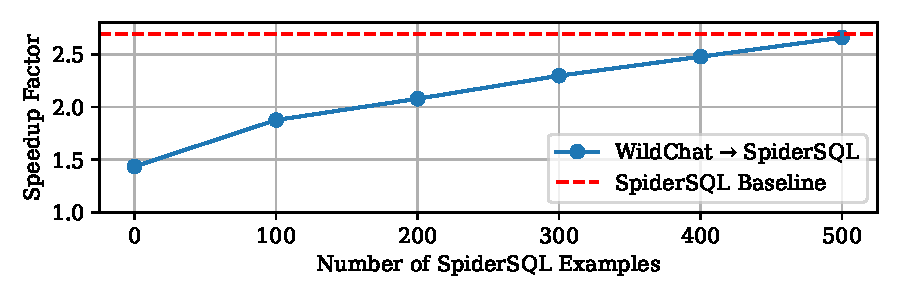
\includegraphics[width=\linewidth,trim={5 5 5 5},clip]{figures/suffixdecoding/distribution_shift_speedup.pdf}
\caption{Speedup.}
\label{suffixdecoding:fig:distribution-shift-speedup}
\end{subfigure}
\par\medskip
\begin{subfigure}[t]{0.85\linewidth}
\centering
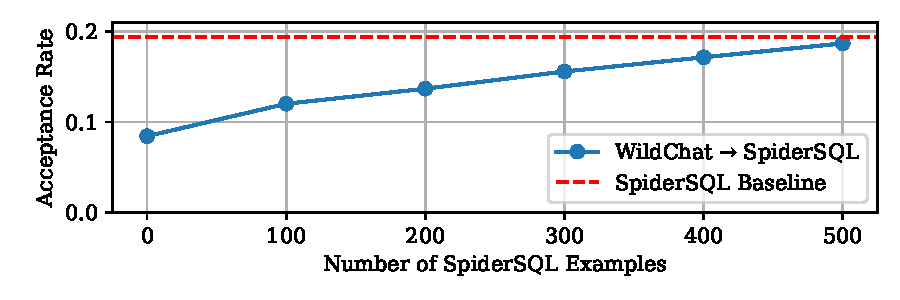
\includegraphics[width=\linewidth,trim={5 5 5 5},clip]{figures/suffixdecoding/distribution_shift_acceptance.pdf}
\caption{Acceptance rate.}
\label{suffixdecoding:fig:distribution-shift-acceptance}
\end{subfigure}
\caption{Speedup (top) and acceptance rate (bottom) of \SuffixDecoding under input distribution shift. \SuffixDecoding was trained on outputs from WildChat, while being evaluated on SpiderSQL. X axis: the number of SpiderSQL inputs, which are added to the global suffix tree after they are processed. Red line: the performance of \SuffixDecoding if trained on 500 output examples from only SpiderSQL offline.}
\label{suffixdecoding:fig:distribution-shift}
\end{figure}

\paragraph{Predicting \SuffixDecoding Effectiveness.}
\label{suffixdecoding:sec:measuring-entropy}

\SuffixDecoding tends to perform better on more structured tasks compared to very open-ended ones (e.g., AgenticSQL vs.\ WildChat). We can measure this ``structuredness'' using empirical entropy. The steps are as follows: (1) create a suffix tree from example model outputs (100 examples is typically enough), (2) calculate the entropy of each node's output distribution by determining how often each child node is accessed, and (3) compute a weighted average of this entropy across all nodes. A low average entropy indicates that output tokens are more predictable based on their prefixes, which generally suggests that \SuffixDecoding will perform better.

\begin{table}[htbp]
\caption{Measured empirical entropy of our various evaluation datasets.}
\label{suffixdecoding:tab:entropy}
\centering
\begin{tabular}{lc}
\toprule
Dataset & Average Entropy \\
\midrule
AgenticSQL (Enrich)   & 0.171 \\
AgenticSQL (Classify) & 0.738 \\
AgenticSQL (Extract)  & 0.0862 \\
AgenticSQL (SQL1)     & 1.52 \\
AgenticSQL (SQL2)     & 1.49 \\
AgenticSQL (SQL3)     & 1.51 \\
AgenticSQL (Combine)  & 1.49 \\
Spider                & 2.50 \\
WildChat              & 3.43 \\
Magicoder             & 2.95 \\
\bottomrule
\end{tabular}
\end{table}

\Cref{suffixdecoding:tab:entropy} shows the empirical entropy measured on samples from each of our evaluation datasets. We find that the average entropy is closely related to the intuitive understanding of the ``structuredness'' of each dataset. Additionally, it correlates well with the performance of \SuffixDecoding on those datasets. Therefore, practitioners can calculate this value using a small number of output examples to assess whether \SuffixDecoding is appropriate for their specific tasks.

\subsection{Scalability and Memory Overhead}
\label{suffixdecoding:sec:scalability}

The suffix trees employed by \SuffixDecoding are highly time and memory efficient. \Cref{suffixdecoding:tab:scalability} shows the per-token lookup time, update time, and memory consumption across various tree sizes (using requests from the SWE-Bench dataset).

\begin{table}[htbp]
\centering
\caption{Suffix tree memory footprint and per-token update and lookup times for different numbers of cached entries (SWE-Bench requests).}
\label{suffixdecoding:tab:scalability}
\small
\begin{tabular}{ccccc}
\toprule
Total \# entries & Total \# tokens & Memory footprint & Avg update time & Avg lookup time \\
                 &                 & (MB)             & per token ($\mu$s)  & per speculated token ($\mu$s) \\
\midrule
1 K entries & 27 M & 1670 MB & 3.95 & 12.18 \\
5 K entries & 143 M & 2980 MB & 4.06 & 10.93 \\
10 K entries & 285 M & 4070 MB & 4.05 & 12.00 \\
15 K entries & 429 M & 5110 MB & 4.07 & 11.62 \\
20 K entries & 572 M & 6150 MB & 4.04 & 11.64 \\
\bottomrule
\end{tabular}
\end{table}

Overall, the total memory consumption scales linearly with the size of the tree, and both the update and lookup times remain fast even with larger trees. Given typical server configurations, \SuffixDecoding can cache many weeks of generated tokens before hitting CPU memory limits. For example, optimized inference engines running Llama-8B on an A100 GPU can typically generate $\sim 5000$ tokens per second~\citep{yin2024sglang} or $\sim 432$M tokens per day. Typical A100 systems (e.g., AWS \texttt{p4d.24xlarge}) have 144GB of CPU memory per A100 GPU. This means that \SuffixDecoding can potentially cache 31 days of generated tokens per A100 GPU before hitting CPU memory limits, as the following calculation shows:
\begin{enumerate}
    \item Memory per token: $6.15~\text{GB} \div 572\text{M tokens} = 1.075 \times 10^{-8}~\text{GB/token}$;
    \item Total token capacity: $144~\text{GB} \div (1.075 \times 10^{-8}~\text{GB/token}) = 1.34 \times 10^{10}~\text{tokens}$;
    \item Time to fill: $(1.34 \times 10^{10}~\text{tokens}) \div (5000~\text{tok/s}) = 2.68 \times 10^{6}~\text{seconds} = 31.0~\text{days}$.
\end{enumerate}
Beyond this limit, it is also straightforward to incorporate cache eviction (e.g., LRU) into \SuffixDecoding to avoid out-of-memory problems.

\subsection{Hybrid Fallback Threshold Sensitivity}
\label{suffixdecoding:sec:threshold-sensitivity}

The hybrid \SuffixDecoding approach (\Cref{suffixdecoding:sec:hybrid}) uses a fallback threshold $\tau$ to determine when to use suffix-tree-based speculation versus falling back to a model-based speculator (e.g., EAGLE-3). This section analyzes the sensitivity of performance to different threshold values across both open-ended and agentic workloads.

\Cref{suffixdecoding:tab:threshold-specbench} shows the wall-clock speedup results on Spec-Bench for various threshold values. For open-ended generation tasks, we find that setting $\tau$ close to or slightly exceeding the mean accepted tokens (MAT) of the model-based speculator yields the best performance. For instance, EAGLE-3 achieves a MAT of approximately 4.65 tokens/step on Spec-Bench. The results show that $\tau \in [5, 7]$ produces the highest overall speedups ($2.5\times$), with performance being relatively stable across this range.

\begin{table}[htbp]
\centering
\caption{Hybrid \SuffixDecoding speedup on Spec-Bench across different threshold values $\tau$.}
\label{suffixdecoding:tab:threshold-specbench}
\small
\begin{tabular}{lccccccc}
\toprule
$\tau$ & coding & qa & math & reasoning & stem & writing & Overall \\
\midrule
7 & 3.44 & 2.40 & 3.14 & 2.50 & 2.87 & 2.83 & 2.50 \\
6 & 3.19 & 2.22 & 2.88 & 2.30 & 2.68 & 2.61 & 2.31 \\
5 & 3.25 & 2.28 & 2.70 & 2.35 & 2.74 & 2.70 & 2.37 \\
4 & 3.07 & 2.22 & 2.72 & 2.25 & 2.57 & 2.64 & 2.25 \\
3 & 2.88 & 2.09 & 2.54 & 2.10 & 2.39 & 2.50 & 2.13 \\
2 & 2.73 & 2.04 & 2.40 & 2.01 & 2.19 & 2.36 & 2.03 \\
1 & 2.28 & 1.86 & 2.01 & 1.69 & 1.90 & 2.12 & 1.80 \\
0 (suffix only) & 1.83 & 1.77 & 1.97 & 1.39 & 1.39 & 1.33 & 1.66 \\
\bottomrule
\end{tabular}
\end{table}

Conversely, \Cref{suffixdecoding:tab:threshold-agenticsql} shows results for AgenticSQL, a highly repetitive agentic workload. Here, the standalone \SuffixDecoding ($\tau = 0$) achieves the best overall speedup ($5.35\times$), as it can confidently speculate much longer sequences than model-based methods. Higher threshold values progressively degrade performance as the system increasingly falls back to less effective model-based speculation.

\begin{table}[htbp]
\centering
\caption{Hybrid \SuffixDecoding speedup on AgenticSQL across different threshold values $\tau$.}
\label{suffixdecoding:tab:threshold-agenticsql}
\small
\begin{tabular}{lcccccc}
\toprule
$\tau$ & Classify & Extract & Enrich & Combine & SQL & Overall \\
\midrule
0 (suffix only) & 3.02 & 9.85 & 10.41 & 4.85 & 3.09 & 5.35 \\
1 & 2.31 & 7.03 & 8.37 & 3.38 & 2.17 & 3.95 \\
2 & 2.24 & 7.14 & 7.97 & 3.33 & 2.29 & 3.80 \\
3 & 2.22 & 5.51 & 5.68 & 3.52 & 2.20 & 3.22 \\
7 & 2.06 & 6.79 & 7.10 & 3.44 & 2.29 & 3.66 \\
\bottomrule
\end{tabular}
\end{table}

In summary, practitioners should set $\tau \approx \text{MAT}_{\text{fallback}}$ for mixed or open-ended workloads, where $\text{MAT}_{\text{fallback}}$ is the mean accepted tokens of the fallback model-based speculator. For highly repetitive agentic workloads, using \SuffixDecoding alone ($\tau = 0$ or very low values) yields the best performance.

\subsection{Detailed Per-Task Results}
\label{suffixdecoding:sec:detailed-results}

The following tables present detailed performance metrics across all evaluation benchmarks, complementing the aggregate results of \Cref{suffixdecoding:fig:throughput-tpot}. For each of SWE-Bench (\Crefrange{suffixdecoding:tab:swe-mat}{suffixdecoding:tab:swe-speedup}), AgenticSQL (\Crefrange{suffixdecoding:tab:sql-mat}{suffixdecoding:tab:sql-speedup}), and Spec-Bench (\Crefrange{suffixdecoding:tab:spec-mat}{suffixdecoding:tab:spec-speedup}), we report the mean accepted tokens per step, the mean acceptance rate (the fraction of speculated tokens that are accepted), the wall-clock time per output token, the speculation time per generated token, and the resulting speedup over vanilla decoding. For Spec-Bench, the 13 categories include both single-turn open-ended tasks (qa, rag, math\_reasoning, summarization, translation) and multi-turn tasks. Eight of these categories (Writing, Roleplay, Reasoning, Math, Coding, Extraction, STEM, Humanities) are from MT-Bench~\citep{mtbench}, allowing direct performance comparison on this widely-used benchmark. The ``Suffix'' rows correspond to standalone \SuffixDecoding and the ``Hybrid'' rows to \SuffixDecoding combined with EAGLE-3, each in both the tree and linear speculation variants.

\begin{table}[htbp]
\centering
\caption{SWE-Bench: mean accepted tokens (tokens/step) for \SuffixDecoding and all baselines, broken down by repository (Llama-3.1-8B-Instruct, one H100 GPU, batch size 1). EAGLE-2/3 and the hybrid variants could not run on SWE-Bench because of its long contexts (over 8192 tokens), and Token Recycling failed on some repositories; the corresponding rows and cells are omitted or marked with a dash.}
\label{suffixdecoding:tab:swe-mat}
\small
\begin{adjustbox}{width=\linewidth}
\begin{tabular}{lccccccccccccc}
\toprule
\textbf{System} & astropy & django & matplotlib & seaborn & flask & requests & xarray & pylint & pytest & scikit-learn & sphinx & sympy & \textbf{Overall} \\
\midrule
Suffix (linear) & 6.415 & 6.546 & 5.521 & 7.207 & 3.772 & 6.480 & 7.137 & 4.635 & 5.412 & 5.933 & 17.140 & 5.165 & 7.821 \\
Suffix (tree) & 6.262 & 6.221 & 4.992 & 7.064 & 3.708 & 5.922 & 6.764 & 4.452 & 5.311 & 5.600 & 16.876 & 5.020 & 7.552 \\
PLD & 2.831 & 3.008 & 2.756 & 3.080 & 2.195 & 2.996 & 3.223 & 2.629 & 2.904 & 2.669 & 4.724 & 2.641 & 3.168 \\
Token Recycling & 3.159 & 3.058 & 3.004 & 3.133 & - & - & 2.978 & 3.072 & 2.992 & 3.046 & 2.994 & - & 3.054 \\
Vanilla & 1.000 & 1.000 & 1.000 & 1.000 & 1.000 & 1.000 & 1.000 & 1.000 & 1.000 & 1.000 & 1.000 & 1.000 & 1.000 \\
\bottomrule
\end{tabular}
\end{adjustbox}
\end{table}

\begin{table}[htbp]
\centering
\caption{SWE-Bench: mean acceptance rate for \SuffixDecoding and all baselines, broken down by repository (Llama-3.1-8B-Instruct, one H100 GPU, batch size 1). Methods that could not run on SWE-Bench are omitted (see \Cref{suffixdecoding:tab:swe-mat}).}
\label{suffixdecoding:tab:swe-rate}
\small
\begin{adjustbox}{width=\linewidth}
\begin{tabular}{lccccccccccccc}
\toprule
\textbf{System} & astropy & django & matplotlib & seaborn & flask & requests & xarray & pylint & pytest & scikit-learn & sphinx & sympy & \textbf{Overall} \\
\midrule
Suffix (linear) & 0.252 & 0.255 & 0.238 & 0.293 & 0.167 & 0.250 & 0.281 & 0.204 & 0.230 & 0.243 & 0.554 & 0.217 & 0.296 \\
Suffix (tree) & 0.235 & 0.230 & 0.195 & 0.272 & 0.153 & 0.222 & 0.250 & 0.183 & 0.217 & 0.216 & 0.539 & 0.196 & 0.274 \\
PLD & 0.191 & 0.210 & 0.184 & 0.215 & 0.128 & 0.208 & 0.231 & 0.174 & 0.199 & 0.175 & 0.379 & 0.175 & 0.225 \\
Token Recycling & 0.028 & 0.027 & 0.026 & 0.028 & - & - & 0.025 & 0.027 & 0.025 & 0.026 & 0.026 & - & 0.026 \\
\bottomrule
\end{tabular}
\end{adjustbox}
\end{table}

\begin{table}[htbp]
\centering
\caption{SWE-Bench: time per output token (ms) for \SuffixDecoding and all baselines, broken down by repository (Llama-3.1-8B-Instruct, one H100 GPU, batch size 1). Methods that could not run on SWE-Bench are omitted (see \Cref{suffixdecoding:tab:swe-mat}).}
\label{suffixdecoding:tab:swe-tpot}
\small
\begin{adjustbox}{width=\linewidth}
\begin{tabular}{lccccccccccccc}
\toprule
\textbf{System} & astropy & django & matplotlib & seaborn & flask & requests & xarray & pylint & pytest & scikit-learn & sphinx & sympy & \textbf{Overall} \\
\midrule
Suffix (linear) & 30.563 & 21.881 & 26.013 & 37.012 & 22.238 & 23.828 & 23.598 & 27.739 & 29.313 & 31.949 & 25.613 & 17.072 & 27.436 \\
Suffix (tree) & 30.800 & 22.238 & 26.278 & 37.095 & 22.728 & 23.998 & 23.847 & 28.388 & 29.451 & 32.496 & 25.853 & 17.199 & 27.711 \\
PLD & 41.675 & 31.029 & 34.447 & 47.588 & 31.549 & 31.155 & 31.330 & 37.386 & 38.238 & 41.531 & 41.877 & 25.142 & 37.758 \\
Token Recycling & 41.328 & 31.847 & 34.155 & 49.670 & - & - & 33.434 & 34.304 & 38.438 & 39.667 & 78.153 & - & 43.774 \\
Vanilla & 50.080 & 41.102 & 43.019 & 57.069 & 35.040 & 39.268 & 41.213 & 42.107 & 45.633 & 46.061 & 77.815 & 32.527 & 50.074 \\
\bottomrule
\end{tabular}
\end{adjustbox}
\end{table}

\begin{table}[htbp]
\centering
\caption{SWE-Bench: speculation time per generated token (ms) for \SuffixDecoding and all baselines, broken down by repository (Llama-3.1-8B-Instruct, one H100 GPU, batch size 1). Methods that could not run on SWE-Bench are omitted (see \Cref{suffixdecoding:tab:swe-mat}).}
\label{suffixdecoding:tab:swe-spectime}
\small
\begin{adjustbox}{width=\linewidth}
\begin{tabular}{lccccccccccccc}
\toprule
\textbf{System} & astropy & django & matplotlib & seaborn & flask & requests & xarray & pylint & pytest & scikit-learn & sphinx & sympy & \textbf{Overall} \\
\midrule
Vanilla & 0.000 & 0.000 & 0.000 & 0.000 & 0.000 & 0.000 & 0.000 & 0.000 & 0.000 & 0.000 & 0.000 & 0.000 & 0.000 \\
Suffix (linear) & 0.156 & 0.122 & 0.175 & 0.185 & 0.198 & 0.182 & 0.178 & 0.203 & 0.217 & 0.203 & 0.125 & 0.167 & 0.171 \\
Suffix (tree) & 0.170 & 0.135 & 0.172 & 0.172 & 0.191 & 0.165 & 0.165 & 0.235 & 0.235 & 0.212 & 0.138 & 0.150 & 0.175 \\
PLD & 0.191 & 0.197 & 0.208 & 0.176 & 0.266 & 0.200 & 0.191 & 0.222 & 0.208 & 0.228 & 0.126 & 0.217 & 0.191 \\
Token Recycling & 9.298 & 6.023 & 7.982 & 13.731 & - & - & 6.607 & 7.665 & 8.081 & 11.748 & 19.653 & - & 10.582 \\
\bottomrule
\end{tabular}
\end{adjustbox}
\end{table}

\begin{table}[htbp]
\centering
\caption{SWE-Bench: speedup over vanilla decoding for \SuffixDecoding and all baselines, broken down by repository (Llama-3.1-8B-Instruct, one H100 GPU, batch size 1). Methods that could not run on SWE-Bench are omitted (see \Cref{suffixdecoding:tab:swe-mat}).}
\label{suffixdecoding:tab:swe-speedup}
\small
\begin{adjustbox}{width=\linewidth}
\begin{tabular}{lccccccccccccc}
\toprule
\textbf{System} & astropy & django & matplotlib & seaborn & flask & requests & xarray & pylint & pytest & scikit-learn & sphinx & sympy & \textbf{Overall} \\
\midrule
Suffix (linear) & 2.213 & 2.442 & 2.039 & 1.951 & 1.792 & 1.962 & 2.210 & 1.792 & 1.888 & 2.356 & 4.453 & 2.292 & 2.452 \\
Suffix (tree) & 2.158 & 2.412 & 1.991 & 1.985 & 1.759 & 1.972 & 2.190 & 1.754 & 1.912 & 2.296 & 4.417 & 2.280 & 2.433 \\
PLD & 1.440 & 1.516 & 1.425 & 1.360 & 1.242 & 1.399 & 1.486 & 1.270 & 1.326 & 1.429 & 2.006 & 1.483 & 1.495 \\
Token Recycling & 1.427 & 1.458 & 1.483 & 1.264 & - & - & 1.360 & 1.311 & 1.290 & 1.399 & 1.328 & - & 1.358 \\
Vanilla & 1.000 & 1.000 & 1.000 & 1.000 & 1.000 & 1.000 & 1.000 & 1.000 & 1.000 & 1.000 & 1.000 & 1.000 & 1.000 \\
\bottomrule
\end{tabular}
\end{adjustbox}
\end{table}

\begin{table}[htbp]
\centering
\caption{AgenticSQL: mean accepted tokens (tokens/step) for \SuffixDecoding and all baselines, broken down by sub-task (Llama-3.1-8B-Instruct, one H100 GPU, batch size 1).}
\label{suffixdecoding:tab:sql-mat}
\small
\begin{adjustbox}{width=\linewidth}
\begin{tabular}{lcccccccc}
\toprule
\textbf{System} & Classify & Extract & Enrich & Combine & SQL1 & SQL2 & SQL3 & \textbf{Overall} \\
\midrule
Hybrid (tree) & 4.180 & 14.813 & 15.081 & 6.448 & 3.983 & 3.932 & 4.006 & 7.500 \\
Hybrid (linear) & 4.008 & 13.473 & 15.304 & 6.362 & 3.876 & 3.842 & 3.913 & 7.262 \\
Suffix (linear) & 3.577 & 11.833 & 12.395 & 5.924 & 3.665 & 3.005 & 4.005 & 6.349 \\
Suffix (tree) & 3.470 & 11.724 & 12.137 & 5.834 & 3.633 & 2.914 & 3.904 & 6.236 \\
EAGLE-2 & 3.156 & 5.173 & 3.249 & 3.534 & 3.066 & 3.761 & 3.057 & 3.572 \\
Token Recycling & 2.915 & 4.125 & 3.125 & 3.138 & 2.951 & 2.929 & 2.994 & 3.169 \\
EAGLE-3 & 2.529 & 3.374 & 4.198 & 3.179 & 2.142 & 4.622 & 2.056 & 3.160 \\
EAGLE & 2.305 & 4.062 & 2.877 & 3.127 & 2.166 & 3.295 & 2.109 & 2.851 \\
PLD & 1.427 & 4.134 & 1.455 & 3.914 & 2.074 & 1.452 & 2.151 & 2.373 \\
Vanilla & 1.000 & 1.000 & 1.000 & 1.000 & 1.000 & 1.000 & 1.000 & 1.000 \\
\bottomrule
\end{tabular}
\end{adjustbox}
\end{table}

\begin{table}[htbp]
\centering
\caption{AgenticSQL: mean acceptance rate for \SuffixDecoding and all baselines, broken down by sub-task (Llama-3.1-8B-Instruct, one H100 GPU, batch size 1).}
\label{suffixdecoding:tab:sql-rate}
\small
\begin{adjustbox}{width=\linewidth}
\begin{tabular}{lcccccccc}
\toprule
\textbf{System} & Classify & Extract & Enrich & Combine & SQL1 & SQL2 & SQL3 & \textbf{Overall} \\
\midrule
Suffix (linear) & 0.212 & 0.628 & 0.740 & 0.428 & 0.318 & 0.245 & 0.330 & 0.415 \\
Suffix (tree) & 0.189 & 0.605 & 0.614 & 0.397 & 0.294 & 0.225 & 0.298 & 0.375 \\
Hybrid (tree) & 0.131 & 0.642 & 0.683 & 0.249 & 0.138 & 0.143 & 0.140 & 0.304 \\
Hybrid (linear) & 0.124 & 0.595 & 0.750 & 0.242 & 0.130 & 0.139 & 0.133 & 0.302 \\
PLD & 0.061 & 0.365 & 0.069 & 0.355 & 0.137 & 0.076 & 0.144 & 0.173 \\
EAGLE & 0.052 & 0.122 & 0.075 & 0.085 & 0.047 & 0.092 & 0.044 & 0.074 \\
EAGLE-2 & 0.036 & 0.070 & 0.037 & 0.042 & 0.034 & 0.046 & 0.034 & 0.043 \\
EAGLE-3 & 0.025 & 0.040 & 0.053 & 0.036 & 0.019 & 0.060 & 0.018 & 0.036 \\
Token Recycling & 0.025 & 0.041 & 0.028 & 0.027 & 0.025 & 0.024 & 0.026 & 0.028 \\
\bottomrule
\end{tabular}
\end{adjustbox}
\end{table}

\begin{table}[htbp]
\centering
\caption{AgenticSQL: time per output token (ms) for \SuffixDecoding and all baselines, broken down by sub-task (Llama-3.1-8B-Instruct, one H100 GPU, batch size 1).}
\label{suffixdecoding:tab:sql-tpot}
\small
\begin{adjustbox}{width=\linewidth}
\begin{tabular}{lcccccccc}
\toprule
\textbf{System} & Classify & Extract & Enrich & Combine & SQL1 & SQL2 & SQL3 & \textbf{Overall} \\
\midrule
Suffix (linear) & 9.552 & 2.687 & 3.007 & 6.023 & 9.559 & 10.588 & 9.767 & 7.306 \\
Suffix (tree) & 9.594 & 2.876 & 3.188 & 6.164 & 10.339 & 10.935 & 10.090 & 7.592 \\
Hybrid (tree) & 11.975 & 3.491 & 3.633 & 7.883 & 14.329 & 11.600 & 14.399 & 9.604 \\
Token Recycling & 10.316 & 7.314 & 9.470 & 9.724 & 10.981 & 9.981 & 10.702 & 9.782 \\
Hybrid (linear) & 12.563 & 3.681 & 3.762 & 8.603 & 14.827 & 11.639 & 21.219 & 10.874 \\
EAGLE-2 & 16.814 & 9.210 & 15.078 & 13.877 & 17.967 & 12.312 & 17.531 & 14.677 \\
PLD & 20.146 & 7.735 & 20.321 & 8.173 & 14.605 & 20.546 & 14.646 & 15.169 \\
EAGLE & 21.221 & 11.308 & 15.760 & 15.688 & 23.353 & 13.396 & 24.595 & 17.887 \\
EAGLE-3 & 23.334 & 14.729 & 12.513 & 16.863 & 26.997 & 10.747 & 27.728 & 18.966 \\
Vanilla & 26.578 & 25.292 & 25.032 & 25.406 & 27.011 & 25.851 & 26.307 & 25.924 \\
\bottomrule
\end{tabular}
\end{adjustbox}
\end{table}

\begin{table}[htbp]
\centering
\caption{AgenticSQL: speculation time per generated token (ms) for \SuffixDecoding and all baselines, broken down by sub-task (Llama-3.1-8B-Instruct, one H100 GPU, batch size 1).}
\label{suffixdecoding:tab:sql-spectime}
\small
\begin{adjustbox}{width=\linewidth}
\begin{tabular}{lcccccccc}
\toprule
\textbf{System} & Classify & Extract & Enrich & Combine & SQL1 & SQL2 & SQL3 & \textbf{Overall} \\
\midrule
Vanilla & 0.000 & 0.000 & 0.000 & 0.000 & 0.000 & 0.000 & 0.000 & 0.000 \\
Suffix (linear) & 0.060 & 0.015 & 0.015 & 0.033 & 0.059 & 0.058 & 0.061 & 0.043 \\
Suffix (tree) & 0.064 & 0.017 & 0.020 & 0.035 & 0.064 & 0.062 & 0.064 & 0.047 \\
PLD & 0.419 & 0.124 & 0.422 & 0.130 & 0.281 & 0.434 & 0.276 & 0.298 \\
Token Recycling & 0.762 & 0.303 & 0.399 & 0.577 & 0.928 & 0.260 & 0.922 & 0.592 \\
Hybrid (tree) & 1.728 & 0.249 & 0.376 & 1.112 & 2.350 & 0.927 & 2.372 & 1.299 \\
Hybrid (linear) & 1.776 & 0.256 & 0.358 & 1.177 & 2.387 & 0.930 & 4.389 & 1.604 \\
EAGLE & 3.189 & 1.693 & 2.423 & 2.372 & 3.423 & 2.197 & 3.616 & 2.700 \\
EAGLE-2 & 4.118 & 2.006 & 3.292 & 3.308 & 4.599 & 2.597 & 4.509 & 3.487 \\
EAGLE-3 & 6.092 & 3.526 & 3.021 & 4.350 & 7.156 & 2.543 & 7.332 & 4.854 \\
\bottomrule
\end{tabular}
\end{adjustbox}
\end{table}

\begin{table}[htbp]
\centering
\caption{AgenticSQL: speedup over vanilla decoding for \SuffixDecoding and all baselines, broken down by sub-task (Llama-3.1-8B-Instruct, one H100 GPU, batch size 1).}
\label{suffixdecoding:tab:sql-speedup}
\small
\begin{adjustbox}{width=\linewidth}
\begin{tabular}{lcccccccc}
\toprule
\textbf{System} & Classify & Extract & Enrich & Combine & SQL1 & SQL2 & SQL3 & \textbf{Overall} \\
\midrule
Suffix (linear) & 3.016 & 9.854 & 10.406 & 4.848 & 3.205 & 2.839 & 3.211 & 5.345 \\
Suffix (tree) & 2.998 & 9.545 & 10.009 & 4.765 & 3.008 & 2.733 & 3.133 & 5.175 \\
Hybrid (tree) & 2.338 & 7.672 & 8.191 & 3.613 & 2.057 & 2.496 & 2.077 & 4.068 \\
Hybrid (linear) & 2.243 & 7.137 & 7.965 & 3.327 & 1.993 & 2.483 & 1.405 & 3.799 \\
Token Recycling & 2.588 & 3.472 & 2.672 & 2.640 & 2.502 & 2.604 & 2.492 & 2.710 \\
PLD & 1.330 & 3.695 & 1.255 & 3.298 & 1.936 & 1.311 & 1.905 & 2.105 \\
EAGLE-2 & 1.591 & 2.751 & 1.673 & 1.855 & 1.527 & 2.119 & 1.527 & 1.864 \\
EAGLE-3 & 1.328 & 1.720 & 2.025 & 1.619 & 1.108 & 2.496 & 1.056 & 1.623 \\
EAGLE & 1.324 & 2.246 & 1.598 & 1.669 & 1.229 & 1.955 & 1.138 & 1.595 \\
Vanilla & 1.000 & 1.000 & 1.000 & 1.000 & 1.000 & 1.000 & 1.000 & 1.000 \\
\bottomrule
\end{tabular}
\end{adjustbox}
\end{table}

\begin{table}[htbp]
\centering
\caption{Spec-Bench: mean accepted tokens (tokens/step) for \SuffixDecoding and all baselines, broken down by category (Llama-3.1-8B-Instruct, one H100 GPU, batch size 1).}
\label{suffixdecoding:tab:spec-mat}
\small
\begin{adjustbox}{width=\linewidth}
\begin{tabular}{lcccccccccccccc}
\toprule
\textbf{System} & coding & extraction & humanities & math & math\_reasoning & qa & rag & reasoning & roleplay & stem & summarization & translation & writing & \textbf{Overall} \\
\midrule
Hybrid (tree) & 6.325 & 5.418 & 4.980 & 5.817 & 5.080 & 4.958 & 4.812 & 4.610 & 4.556 & 5.155 & 4.550 & 3.432 & 5.306 & 4.684 \\
EAGLE-3 & 5.975 & 5.373 & 5.180 & 5.745 & 5.562 & 4.351 & 5.009 & 4.956 & 4.664 & 5.299 & 4.767 & 2.909 & 5.093 & 4.647 \\
Hybrid (linear) & 5.958 & 5.249 & 4.966 & 5.446 & 5.121 & 4.452 & 4.753 & 4.607 & 4.557 & 5.089 & 4.520 & 3.345 & 5.158 & 4.553 \\
EAGLE-2 & 4.766 & 3.842 & 3.612 & 4.242 & 4.129 & 3.324 & 3.630 & 3.892 & 3.353 & 3.736 & 3.254 & 2.605 & 3.383 & 3.466 \\
EAGLE & 4.149 & 3.469 & 3.177 & 3.724 & 3.617 & 2.857 & 3.239 & 3.328 & 2.968 & 3.311 & 2.926 & 2.352 & 3.082 & 3.065 \\
Token Recycling & 3.044 & 2.610 & 2.539 & 3.128 & 2.980 & 2.372 & 2.352 & 2.537 & 2.338 & 2.697 & 2.614 & 2.305 & 2.417 & 2.548 \\
Suffix (linear) & 1.981 & 1.757 & 1.454 & 2.161 & 1.661 & 1.878 & 1.999 & 1.521 & 1.252 & 1.485 & 1.725 & 1.705 & 1.435 & 1.766 \\
Suffix (tree) & 1.960 & 1.754 & 1.461 & 2.134 & 1.638 & 1.874 & 1.957 & 1.504 & 1.259 & 1.501 & 1.703 & 1.705 & 1.424 & 1.750 \\
PLD & 1.911 & 1.670 & 1.387 & 1.957 & 1.475 & 1.461 & 1.967 & 1.490 & 1.206 & 1.430 & 1.816 & 1.362 & 1.394 & 1.606 \\
Vanilla & 1.000 & 1.000 & 1.000 & 1.000 & 1.000 & 1.000 & 1.000 & 1.000 & 1.000 & 1.000 & 1.000 & 1.000 & 1.000 & 1.000 \\
\bottomrule
\end{tabular}
\end{adjustbox}
\end{table}

\begin{table}[htbp]
\centering
\caption{Spec-Bench: mean acceptance rate for \SuffixDecoding and all baselines, broken down by category (Llama-3.1-8B-Instruct, one H100 GPU, batch size 1).}
\label{suffixdecoding:tab:spec-rate}
\small
\begin{adjustbox}{width=\linewidth}
\begin{tabular}{lcccccccccccccc}
\toprule
\textbf{System} & coding & extraction & humanities & math & math\_reasoning & qa & rag & reasoning & roleplay & stem & summarization & translation & writing & \textbf{Overall} \\
\midrule
Suffix (linear) & 0.255 & 0.216 & 0.162 & 0.240 & 0.163 & 0.152 & 0.216 & 0.171 & 0.116 & 0.169 & 0.199 & 0.216 & 0.208 & 0.190 \\
Suffix (tree) & 0.244 & 0.211 & 0.156 & 0.232 & 0.149 & 0.144 & 0.203 & 0.156 & 0.115 & 0.165 & 0.189 & 0.208 & 0.194 & 0.179 \\
PLD & 0.132 & 0.097 & 0.063 & 0.126 & 0.071 & 0.088 & 0.119 & 0.076 & 0.037 & 0.068 & 0.103 & 0.130 & 0.072 & 0.099 \\
EAGLE & 0.126 & 0.099 & 0.087 & 0.109 & 0.105 & 0.074 & 0.090 & 0.093 & 0.079 & 0.092 & 0.077 & 0.054 & 0.083 & 0.083 \\
Hybrid (linear) & 0.109 & 0.084 & 0.072 & 0.100 & 0.078 & 0.074 & 0.075 & 0.069 & 0.062 & 0.075 & 0.068 & 0.044 & 0.077 & 0.070 \\
Hybrid (tree) & 0.107 & 0.084 & 0.072 & 0.101 & 0.077 & 0.075 & 0.074 & 0.069 & 0.062 & 0.076 & 0.068 & 0.045 & 0.077 & 0.070 \\
EAGLE-3 & 0.083 & 0.073 & 0.070 & 0.079 & 0.076 & 0.056 & 0.067 & 0.066 & 0.061 & 0.072 & 0.063 & 0.032 & 0.068 & 0.061 \\
EAGLE-2 & 0.063 & 0.047 & 0.044 & 0.054 & 0.052 & 0.039 & 0.044 & 0.048 & 0.039 & 0.046 & 0.038 & 0.027 & 0.040 & 0.041 \\
Token Recycling & 0.026 & 0.020 & 0.019 & 0.027 & 0.025 & 0.017 & 0.017 & 0.020 & 0.017 & 0.021 & 0.020 & 0.017 & 0.018 & 0.020 \\
\bottomrule
\end{tabular}
\end{adjustbox}
\end{table}

\begin{table}[htbp]
\centering
\caption{Spec-Bench: time per output token (ms) for \SuffixDecoding and all baselines, broken down by category (Llama-3.1-8B-Instruct, one H100 GPU, batch size 1).}
\label{suffixdecoding:tab:spec-tpot}
\small
\begin{adjustbox}{width=\linewidth}
\begin{tabular}{lcccccccccccccc}
\toprule
\textbf{System} & coding & extraction & humanities & math & math\_reasoning & qa & rag & reasoning & roleplay & stem & summarization & translation & writing & \textbf{Overall} \\
\midrule
Hybrid (linear) & 7.218 & 9.235 & 8.970 & 7.974 & 8.783 & 11.534 & 10.576 & 9.899 & 10.195 & 8.698 & 9.857 & 14.858 & 8.806 & 10.747 \\
Hybrid (tree) & 7.251 & 9.588 & 9.519 & 8.203 & 9.194 & 11.880 & 11.098 & 10.543 & 10.775 & 9.133 & 10.214 & 15.262 & 9.141 & 11.153 \\
Token Recycling & 9.475 & 11.528 & 11.333 & 9.224 & 9.749 & 13.475 & 12.957 & 11.489 & 12.425 & 10.691 & 11.373 & 13.104 & 12.019 & 11.947 \\
EAGLE-2 & 9.721 & 13.256 & 12.822 & 11.157 & 11.338 & 14.903 & 14.012 & 12.631 & 14.229 & 12.461 & 14.422 & 19.116 & 13.992 & 14.387 \\
EAGLE & 10.201 & 13.193 & 13.570 & 11.485 & 11.895 & 16.219 & 14.222 & 13.215 & 14.639 & 13.022 & 14.840 & 19.425 & 14.280 & 14.925 \\
Suffix (tree) & 13.833 & 16.284 & 18.670 & 13.547 & 16.304 & 19.839 & 15.285 & 18.382 & 21.339 & 18.034 & 15.825 & 16.595 & 19.154 & 16.875 \\
Suffix (linear) & 13.595 & 16.245 & 18.212 & 13.292 & 16.447 & 19.999 & 15.378 & 18.061 & 21.217 & 18.041 & 15.925 & 16.670 & 18.925 & 16.936 \\
PLD & 14.681 & 17.524 & 20.469 & 14.450 & 19.179 & 22.693 & 16.383 & 19.173 & 23.300 & 19.714 & 15.949 & 22.214 & 20.438 & 19.190 \\
Vanilla & 24.721 & 24.903 & 24.979 & 24.466 & 24.992 & 25.082 & 25.698 & 24.475 & 24.433 & 24.871 & 25.114 & 24.904 & 24.463 & 25.076 \\
\bottomrule
\end{tabular}
\end{adjustbox}
\end{table}

\begin{table}[htbp]
\centering
\caption{Spec-Bench: speculation time per generated token (ms) for \SuffixDecoding and all baselines, broken down by category (Llama-3.1-8B-Instruct, one H100 GPU, batch size 1).}
\label{suffixdecoding:tab:spec-spectime}
\small
\begin{adjustbox}{width=\linewidth}
\begin{tabular}{lcccccccccccccc}
\toprule
\textbf{System} & coding & extraction & humanities & math & math\_reasoning & qa & rag & reasoning & roleplay & stem & summarization & translation & writing & \textbf{Overall} \\
\midrule
Vanilla & 0.000 & 0.000 & 0.000 & 0.000 & 0.000 & 0.000 & 0.000 & 0.000 & 0.000 & 0.000 & 0.000 & 0.000 & 0.000 & 0.000 \\
Suffix (linear) & 0.071 & 0.079 & 0.099 & 0.067 & 0.087 & 0.097 & 0.089 & 0.084 & 0.101 & 0.094 & 0.092 & 0.076 & 0.084 & 0.088 \\
Suffix (tree) & 0.074 & 0.080 & 0.104 & 0.069 & 0.091 & 0.099 & 0.093 & 0.088 & 0.103 & 0.097 & 0.096 & 0.079 & 0.086 & 0.091 \\
Token Recycling & 0.243 & 0.318 & 0.291 & 0.240 & 0.255 & 0.391 & 0.419 & 0.304 & 0.320 & 0.275 & 0.321 & 0.365 & 0.310 & 0.340 \\
PLD & 0.291 & 0.357 & 0.421 & 0.277 & 0.392 & 0.480 & 0.326 & 0.391 & 0.492 & 0.407 & 0.325 & 0.466 & 0.428 & 0.395 \\
Hybrid (linear) & 1.369 & 1.838 & 2.026 & 1.510 & 1.854 & 2.455 & 2.152 & 2.070 & 2.353 & 1.925 & 2.118 & 3.096 & 1.949 & 2.259 \\
EAGLE & 1.698 & 1.977 & 2.268 & 1.877 & 1.892 & 2.389 & 2.034 & 2.060 & 2.421 & 2.166 & 2.434 & 2.885 & 2.351 & 2.289 \\
Hybrid (tree) & 1.445 & 1.935 & 2.152 & 1.580 & 1.947 & 2.553 & 2.238 & 2.196 & 2.506 & 2.010 & 2.200 & 3.141 & 2.056 & 2.344 \\
EAGLE-3 & 1.913 & 2.172 & 2.218 & 2.001 & 2.030 & 2.674 & 2.419 & 2.334 & 2.500 & 2.160 & 2.402 & 4.084 & 2.237 & 2.634 \\
EAGLE-2 & 2.055 & 2.656 & 2.714 & 2.338 & 2.346 & 2.962 & 2.807 & 2.584 & 2.997 & 2.628 & 3.062 & 3.826 & 2.946 & 2.936 \\
\bottomrule
\end{tabular}
\end{adjustbox}
\end{table}

\begin{table}[htbp]
\centering
\caption{Spec-Bench: speedup over vanilla decoding for \SuffixDecoding and all baselines, broken down by category (Llama-3.1-8B-Instruct, one H100 GPU, batch size 1).}
\label{suffixdecoding:tab:spec-speedup}
\small
\begin{adjustbox}{width=\linewidth}
\begin{tabular}{lcccccccccccccc}
\toprule
\textbf{System} & coding & extraction & humanities & math & math\_reasoning & qa & rag & reasoning & roleplay & stem & summarization & translation & writing & \textbf{Overall} \\
\midrule
Hybrid (linear) & 3.441 & 2.795 & 2.800 & 3.139 & 2.866 & 2.404 & 2.542 & 2.496 & 2.461 & 2.871 & 2.573 & 1.759 & 2.833 & 2.500 \\
Hybrid (tree) & 3.442 & 2.717 & 2.644 & 3.132 & 2.736 & 2.611 & 2.445 & 2.344 & 2.330 & 2.732 & 2.485 & 1.713 & 2.736 & 2.458 \\
EAGLE-3 & 3.115 & 2.634 & 2.713 & 2.910 & 2.888 & 2.172 & 2.474 & 2.446 & 2.394 & 2.764 & 2.520 & 1.447 & 2.622 & 2.367 \\
Token Recycling & 2.619 & 2.234 & 2.209 & 2.660 & 2.577 & 1.951 & 2.057 & 2.150 & 1.979 & 2.334 & 2.218 & 1.932 & 2.057 & 2.169 \\
EAGLE-2 & 2.548 & 1.998 & 1.958 & 2.215 & 2.220 & 1.733 & 1.877 & 1.968 & 1.751 & 2.007 & 1.756 & 1.336 & 1.791 & 1.825 \\
EAGLE & 2.427 & 1.956 & 1.848 & 2.142 & 2.112 & 1.600 & 1.841 & 1.871 & 1.703 & 1.922 & 1.702 & 1.305 & 1.753 & 1.752 \\
Suffix (tree) & 1.796 & 1.620 & 1.350 & 1.930 & 1.558 & 1.785 & 1.886 & 1.364 & 1.149 & 1.389 & 1.624 & 1.627 & 1.310 & 1.661 \\
Suffix (linear) & 1.828 & 1.630 & 1.383 & 1.967 & 1.544 & 1.773 & 1.890 & 1.389 & 1.156 & 1.386 & 1.618 & 1.618 & 1.327 & 1.659 \\
PLD & 1.712 & 1.484 & 1.231 & 1.753 & 1.323 & 1.326 & 1.807 & 1.320 & 1.055 & 1.275 & 1.628 & 1.219 & 1.232 & 1.448 \\
Vanilla & 1.000 & 1.000 & 1.000 & 1.000 & 1.000 & 1.000 & 1.000 & 1.000 & 1.000 & 1.000 & 1.000 & 1.000 & 1.000 & 1.000 \\
\bottomrule
\end{tabular}
\end{adjustbox}
\end{table}


\section{Discussion}
\label{suffixdecoding:sec:discussion}

\paragraph{Limitations.}
In terms of speculation performance, \SuffixDecoding is limited by its context defined by the prefix sequence it uses to look up candidate tokens. Although \SuffixDecoding performs well in our evaluations, there may be other datasets in which long-range dependencies are more frequent and would be detrimental to \SuffixDecoding's performance. The empirical entropy measure of \Cref{suffixdecoding:sec:measuring-entropy} offers a cheap way to assess, from a small number of output samples, whether a given workload is a good fit.

\paragraph{Privacy Considerations.}
There may be privacy concerns in re-using previously generated outputs to speculate new outputs. We suggest two methods to mitigate this. First, \SuffixDecoding is an exact speculative decoding method, meaning it precisely preserves the original LLM output distribution, even if draft tokens are selected from a different request. We consider this property as a first layer of privacy protection. Second, in real-world enterprise deployments, \SuffixDecoding makes it easy to build and maintain disjoint suffix trees per user or customer of the LLM service. For each user, it is efficient to maintain suffix trees just for the private use of that user.

\paragraph{Batch-Level Speculation Control.}
\label{suffixdecoding:sec:batch-speculation}
For batched serving scenarios, optimizing the speculation per request in a batch is crucial for many practical online deployments. While \SuffixDecoding focuses on \textit{what} tokens to speculate, it is also compatible with existing works that explore \textit{how much} to speculate per request. For example, TurboSpec~\citep{turbospec} uses a ``goodput'' metric to balance speculation lengths and batch size, noting that optimal speculation decreases as batch size increases. AdaServe~\citep{adaserve} formulates multi-SLO serving as a constrained optimization problem and introduces SLO-customized speculative decoding that constructs speculation trees tailored to each request's latency target.
By dynamically adjusting the number of speculative tokens generated from the suffix tree per request, \SuffixDecoding can be integrated with TurboSpec to maximize the batch-wise goodput metric.
Furthermore, the statistics-based scoring used by \SuffixDecoding can potentially better inform methods like TurboSpec, for example by choosing to speculate more from sequences that have a higher marginal score.
These are interesting and important directions for future work.

\section{Related Work}
\label{suffixdecoding:sec:related}

\paragraph{Speculative Decoding.} Speculative decoding~\citep{leviathan2022fast,chen2023accelerating} can improve LLM inference latency without compromising the quality of the generated text. Model-based methods include Medusa~\citep{cai2024medusasimplellminference} and \SpecInfer~\citep{specinfer}, which first introduced tree-based speculation. Medusa uses multiple decoding heads for parallel candidate generation, while \SpecInfer uses multiple draft models or speculative sampling to generate a tree of candidate tokens. EAGLE-2/3~\citep{eagle2,li2025eagle3scalinginferenceacceleration} train lightweight draft heads that reuse the target model's hidden features and build dynamic speculation trees, and Sequoia~\citep{sequoia} optimizes the speculation tree topology for a given hardware setting. Other approaches include multi-token prediction~\citep{gloeckle2024multitoken} and blockwise parallel decoding~\citep{stern2018blockwise,kim2024accelerating}.
There are also several model-free speculation methods, such as Prompt Lookup Decoding~\citep{saxena2023prompt}, Token Recycling~\citep{luo2024turningtrashtreasureaccelerating}, LLMA~\citep{yang2023inference}, and ANPD~\citep{ou2024losslessaccelerationlargelanguage}. These methods rely on small reference texts such as the prompt or retrieved contexts, and lack the adaptive speculation mechanisms of \SuffixDecoding. Compared to prior speculative decoding methods, \SuffixDecoding is uniquely designed for the emerging class of agentic LLM applications.

\paragraph{Methods for Accelerating LLM Agents.} Recent works also target the problem of latency in agentic applications. ALTO~\citep{10.1145/3642970.3655844} takes a systems-oriented approach to optimize the latency of multi-agent workflows through more efficient pipelining and scheduling. Dynasor~\citep{fu2024efficientlyservingllmreasoning} monitors the certainty of agentic reasoning algorithms as they run, and early-terminates reasoning paths that are unlikely to improve the final answer. Compared to these systems, \SuffixDecoding takes an orthogonal speculative decoding approach, and they can be used in combination.

\section{Summary}
\label{suffixdecoding:sec:summary}

In this chapter, we presented \SuffixDecoding, a model-free speculative decoding approach designed for emerging agentic applications. Using efficient suffix tree data structures, \SuffixDecoding effectively exploits long and repetitive token sequences found in many agentic algorithms, such as self-consistency, self-refinement, and multi-agent pipelines. Its adaptive speculation length and frequency-based scoring let it speculate aggressively when the recent context matches historical patterns and conservatively otherwise, and the same scoring function provides a natural hook for a hybrid mode that falls back to model-based speculators on open-ended inputs. Using two practical agentic applications, OpenHands and AgenticSQL, we showed that \SuffixDecoding significantly accelerates their decoding latency and task-completion times, and is also significantly faster than other model-based and model-free speculative decoding baselines.

\chapter{\FastKernels: Benchmarking GPU Kernel Generation in Production}
\label{ch:fastkernels}

% Adapted from reference/papers/fastkernels (FastKernels: Benchmarking GPU
% Kernel Generation in Production). All labels are prefixed with "fastkernels:".
% No chapter-specific macros are needed: the paper's \fastkernels{} macro maps
% to the preamble's \FastKernels, and \textsc{MacroEval} is written inline.
% The paper's appendix has been folded into the body: methodology, setup, and
% supporting results are kept in the relevant sections; exhaustive
% per-architecture and per-model tables are cut and referred to the paper.

\section{Introduction}
\label{fastkernels:sec:introduction}

LLM-based agents for GPU kernel generation now achieve strong scores on isolated benchmarks~\citep{kernelbench,solexecbench,flashinferbench}, with state-of-the-art systems autonomously compiling, profiling, and refining CUDA or Triton code.
Yet these gains often fail to transfer into production inference frameworks such as vLLM~\citep{vllm} and SGLang~\citep{sglang}: kernels that score well in sandbox evaluation routinely regress once they encounter real serving interfaces, compilation stacks, and workloads.

The root cause is \textbf{benchmark--production misalignment}.
Current benchmarks rely heavily on synthetic inputs, single-GPU isolated kernels, simplified interfaces, and independent task levels that do not compose into full inference pipelines.
They therefore reward kernels that are fast in isolation but brittle in deployed systems, hiding interface mismatches, compilation-stack conflicts, and correctness degradation that only appears at model scale.

This chapter introduces \FastKernels, a benchmark of \textbf{384 tasks} drawn from 47 representative architectures across 8 categories, whose kernels suffice to reimplement \textbf{94.6\% (472/499)} of HuggingFace Transformers architectures with outputs matching the native implementations.
Each task mirrors the interface of the corresponding production module and is scored against the kernels production frameworks ship, and tasks form a compositional hierarchy, from primitives to full models, in which higher-level modules import lower-level ones.
Candidates are scored at the kernel level and end to end inside the models they come from, on the production execution path, and \textsc{MacroEval} aggregates calibrated correctness, coverage, and speedup into a leaderboard.
Seeding it with five representative agents (6{,}900 agent-hours), we find that kernel-level speedups of $1.6$--$6.6\times$ shrink to \textbf{at most $1.25\times$} end to end, \textbf{only 20\%} of winning kernel sets run correctly as-is, and kernel-level scores \textbf{mis-rank agents}: Claude Code matches or beats KDA at every level in isolation, yet KDA scores $3\times$ higher end to end.
The benchmark and its evaluation scripts are open source.\footnote{\url{https://github.com/Snowflake-AI-Research/fastkernels}}

\paragraph{Our approach.}
\FastKernels (\Cref{fastkernels:fig:overview}) is a benchmark for kernel agents designed so that its scores predict deployment outcomes.
\FastKernels derives 384 tasks top-down from 47 real model architectures across 8 categories; each task's interface matches the corresponding module in the production library for its family, and each candidate is scored against the kernels that library ships.
Crucially, its task levels are compositional: Level~1 primitives feed Level~2 fused operators, which feed Level~3 layers and Level~4 models.
Unlike benchmarks whose levels are independent, this hierarchy enables a dynamic-programming style optimization loop: an agent can reuse an optimized lower-level kernel, such as a linear operator, when optimizing higher-level modules such as MLPs or transformer blocks, instead of rediscovering the same building block from scratch.

Because integration failures only surface at model scale, \FastKernels also scores every candidate end to end, inside the models its tasks come from and on their production execution path (continuous batching, chunked prefill, CUDA graphs, \texttt{torch.compile}, tensor parallelism).
This model runtime is the benchmark's measurement instrument, not a separate contribution, and we validate it against vLLM, SGLang, and the other production references before scoring any agent (\Cref{fastkernels:sec:eval-results}).
The result is an open leaderboard that ranks agents by what survives deployment, scored with \textsc{MacroEval}, and we seed it with a 6{,}900-agent-hour evaluation of five representative agents, from an RL-trained kernel model to contest-winning long-horizon harnesses.

\begin{figure}[t]
\centering
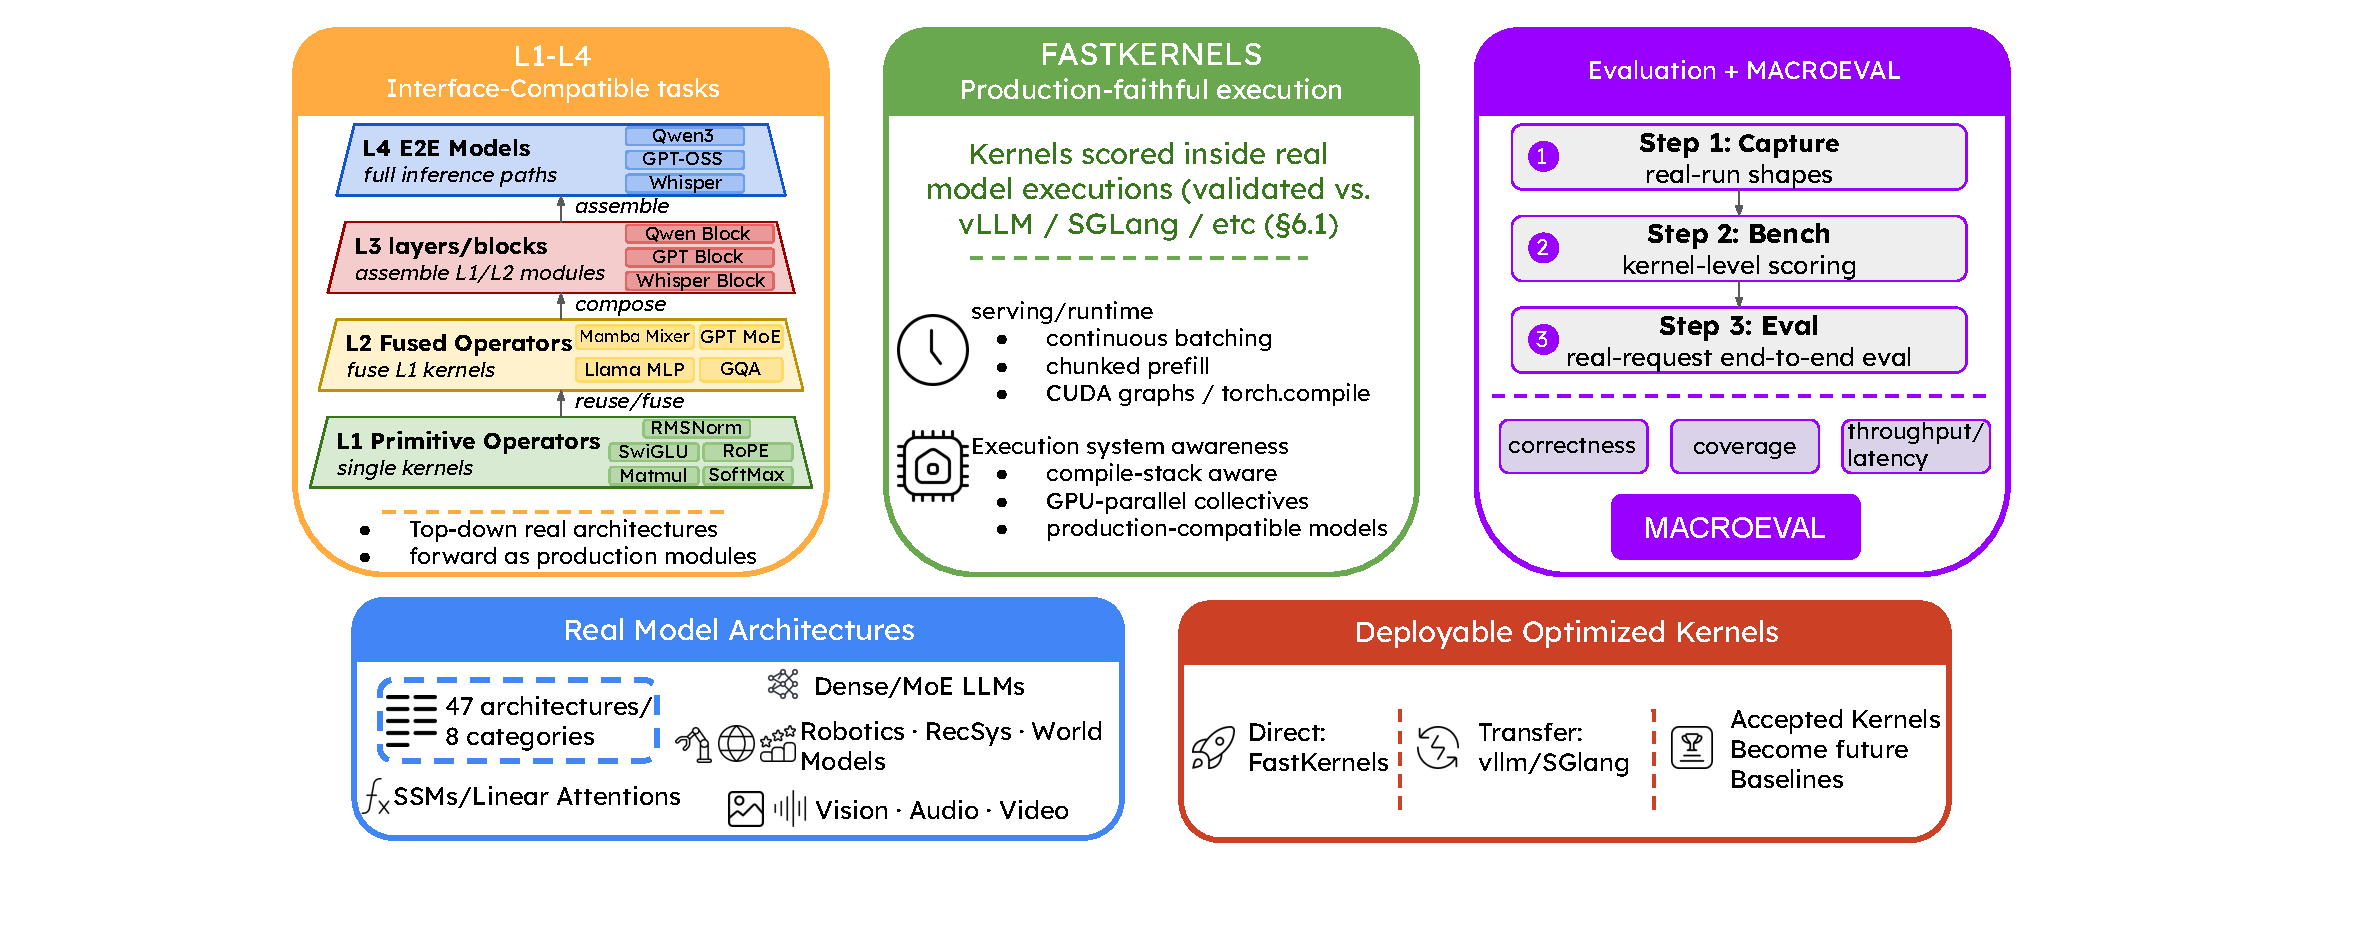
\includegraphics[width=\linewidth]{figures/fastkernels/overview.pdf}
\caption{\textbf{\FastKernels overview.} Tasks derived from 47 real architectures (bottom left) form a compositional L1--L4 hierarchy with production interfaces (top left) and run inside validated production model executions (center). Candidates are scored by capture, kernel-level bench, and end-to-end eval, aggregated by \textsc{MacroEval} (right); optimized kernels deploy directly or transfer into vLLM and SGLang (bottom right).}
\label{fastkernels:fig:overview}
\end{figure}

\paragraph{Contributions.}
This chapter makes the following contributions.
\begin{enumerate}[leftmargin=*, itemsep=2pt, topsep=2pt]
\item \textbf{Production-aligned task suite.}
384 tasks from 47 architectures across 8 categories, from dense and MoE LLMs and SSMs to vision, audio, robotics, 3D, recommendation, and world models, with production module interfaces and speedups measured against production kernels.

\item \textbf{Compositional task hierarchy.}
Unlike flat benchmarks, the primitives-to-models hierarchy exposes \emph{composition effects}: 37\% of the agents' L3 winners break once their own lower-level kernels are active, and regenerating them on frozen lower-level winners yields 80 correct L3 winners instead of 45 (\Cref{fastkernels:sec:eval-agents}).

\item \textbf{Production-faithful evaluation.}
Kernel-level scoring on captured production shapes, with collectives on real tensor-parallel groups, and end-to-end scoring inside full models.

\item \textbf{A deployment-grounded leaderboard.}
\textsc{MacroEval} ranks agents by calibrated correctness, coverage, and end-to-end speedup across model families. Our seed evaluation of five representative agents shows kernel-level speedups of up to $6.6\times$ shrinking to at most $1.25\times$ end to end, and kernel-level scores that mis-rank agents (\Cref{fastkernels:sec:eval-e2e}).
\end{enumerate}

The rest of this chapter is organized as follows.
\Cref{fastkernels:sec:benchmark} describes task construction, the compositional hierarchy, and production-matched interfaces; \Cref{fastkernels:sec:benchmarking_tooling} describes the evaluation stack, its scenario sets, and the workload-capture pipeline; \Cref{fastkernels:sec:metrics} defines \textsc{MacroEval}; and \Cref{fastkernels:sec:evaluation} describes the experimental setup, validates the benchmark, and reports the seed agent evaluation.
\Cref{fastkernels:sec:related} discusses related work and \Cref{fastkernels:sec:summary} concludes.

\section{Benchmark Design}
\label{fastkernels:sec:benchmark}

\FastKernels derives all tasks top-down from real model architectures, ensuring that every kernel can be traced to a specific layer in a specific model and evaluated end-to-end.

\subsection{Top-Down, Model-Driven Construction}
\label{fastkernels:sec:construction}

Unlike prior benchmarks that construct tasks bottom-up by combining primitive operators~\citep{kernelbench} or extracting subgraphs via automated pipelines~\citep{solexecbench}, \FastKernels takes a \emph{top-down} approach.
We begin with real model families---selected to represent the current and near-future frontier of AI workloads---and recursively decompose them into the kernels that constitute their inference paths.

\paragraph{Task construction.}
For each model architecture, we load the HuggingFace configuration and architecture definition, walk the forward pass, and produce standalone task implementations for each computational kernel with all configuration constants (hidden size, number of heads, data types) inlined from the model's configuration.
Every task is then audited to verify: (i)~semantic correctness of the reference implementation, (ii)~that the task captures the operator as it actually executes in the model (not a simplified proxy), (iii)~that tensor shapes and data types match the model's real configuration, and (iv)~that the task's interface matches the corresponding module in the production reference library (\Cref{fastkernels:sec:interface}).
The construction pipeline ships with \FastKernels, so users can add new architectures from HuggingFace with minimal effort.
No task is synthetic: unlike KernelBench's Level-2 random fusions or SOL-ExecBench's LLM-selected subgraphs, every task is an operation that runs in a real model during inference.

\subsection{Task Hierarchy}
\label{fastkernels:sec:hierarchy}

\FastKernels organizes tasks into four levels of increasing scope:

\begin{itemize}[leftmargin=*, itemsep=2pt, topsep=2pt]
\item \textbf{Level 1 --- Primitive operators.}
Individual operations: attention variants (GQA, MLA, sliding-window), normalizations (RMSNorm, LayerNorm), activations (SwiGLU, GeGLU), positional encodings (RoPE, ALiBi), and quantization/dequantization routines.

\item \textbf{Level 2 --- Fused operators.}
Multi-operation kernels representing natural fusion opportunities as they arise in real models: residual-add + RMSNorm + quantization, attention + output projection, MoE gate + dispatch + expert computation.

\item \textbf{Level 3 --- Full layers and blocks.}
Complete architectural blocks: transformer decoder layers, SSM scan blocks, MoE layers with routing, cross-attention layers, and vision encoder stages.

\item \textbf{Level 4 --- End-to-end model architectures.}
Full model inference paths evaluated as integrated systems.
The 47 representative architectures in Level~4 serve as the end-to-end evaluation set, but the underlying L1--L3 kernels cover most operators across ML models.
\end{itemize}

\paragraph{Standalone and composed evaluation.}
Crucially, the hierarchy is not just organizational---it is \emph{executable}.
L2--L4 baselines import their lower-level dependencies via relative imports (e.g., an L3 decoder layer does \texttt{from~..L2.attention~import~Attention}), mirroring how production frameworks assemble modules.
In \emph{standalone} mode (\texttt{-{}-standalone}), each candidate is benched in isolation: imported lower-level modules resolve to their production baselines regardless of what other candidate files exist.
In \emph{composed} mode, all candidate files in the candidate directory are active simultaneously, so an L3 block's lower-level imports resolve to agent-generated candidates rather than production baselines.
The standalone score measures how well the agent optimized one module; the composed score measures what a real deployment would observe when multiple agent-generated modules interact.
The gap between the two---the \emph{composition effect}---is a first-order signal that flat benchmarks are structurally unable to produce (\Cref{fastkernels:sec:eval-agents}).

\subsection{Architecture Coverage}
\label{fastkernels:sec:coverage}

\FastKernels is designed to cover as many model architectures as possible with the \emph{minimum} number of kernels, by consolidating near-identical operators (e.g., RoPE variants, normalizations, attention backends) into a single L1/L2 task and picking a small set of representative architectures whose union of operators subsumes the long tail of model families. The resulting 47 architectures (\Cref{fastkernels:tab:categories}) span 8 categories and precision formats from 1.58-bit through FP32, and comprise 384 unique tasks: 108 L1, 155 L2, and 74 L3 kernel tasks, shared across architectures, plus the 47 end-to-end L4 models (\Cref{fastkernels:fig:arch_pie}).

\begin{table}[t]
  \centering
  \caption{\textbf{Categories and architectures of \FastKernels.} The 47 end-to-end (L4) architectures by category, with the inference precision formats each category exercises.}
  \label{fastkernels:tab:categories}
  \small
  \setlength{\tabcolsep}{4pt}
  \begin{adjustbox}{max width=\linewidth}
  \begin{tabular}{@{}lc>{\raggedright\arraybackslash}p{7.2cm}l@{}}
  \toprule
  \textbf{Category} & \textbf{\#} & \textbf{Architectures} & \textbf{dtypes} \\
  \midrule
  Dense \& MoE LLMs & 7 & Llama-3.1, GLM-5.2, Mixtral, BitNet 1.58b, GPT-OSS, EAGLE-3, Gemma-4 & BF16, W1.58, MXFP4, NVFP4 \\
  Linear attention \& new archs & 9 & Mamba, Mamba2, RWKV-7, GLA, RetNet, Qwen-3-Next, Kimi-Linear, TTT-E2E, Jamba & BF16 \\
  Vision / video / audio & 6 & FLUX.1-Dev, HunyuanVideo-1.5, SDXL, SAM3.1, Whisper, CosyVoice3 & BF16, FP16 \\
  Multimodal \& encoders & 7 & Qwen2-VL, Qwen3-VL-8B, Qwen3-VL-235B, Qwen-2.5-Omni, SigLIP-2, DINOv3, SwinV2 & BF16, FP8, FP32 \\
  Edge \& detection & 5 & MobileNetV4, ConvNeXtV2, EfficientNetV2, YOLOv10, RTDetrV2 & FP32, FP16 \\
  3D / robotics / science & 6 & 3DGS, InstantNGP, PointTransformerV3, OpenFold3, Pi0, DP3 & FP32, FP16, BF16 \\
  Recommendation \& specialized & 5 & DLRMv2, LightGCN, BGE-M3, ColBERTv2, LLaDA & FP32, FP16, BF16 \\
  World models & 2 & Oasis, V-JEPA 2 & BF16 \\
  \bottomrule
  \end{tabular}
  \end{adjustbox}
\end{table}

\paragraph{Counting rule.}
A task is one module file under \texttt{tasks/baseline/L$n$/} that defines at least one benchmarkable \texttt{nn.Module} and is reachable, through the import graph, from at least one of the 47 L4 architectures; it is counted once even when it ships a CUDA sidecar (17 tasks do) or defines several module classes.
Twelve function-only helper kernels (e.g., Triton attention-merge and causal-convolution kernels) are called from inside other tasks and are optimized through them, so they are not counted separately.
L4 counts one task per end-to-end architecture: the encoder sub-models that some pipelines import (the CLIP and T5 text encoders, the Qwen2.5-VL vision encoder) are part of those pipelines' L4 tasks, and the L1--L3 set is identical with or without DeepSeek-V3.2, whose modules GLM-5.2 builds on.
Because tasks are shared, the number of tasks the individual architectures use sums to more than 384.
We refer the reader to the \FastKernels paper~\cite{fastkernels} for the per-architecture breakdown, with the reference checkpoint, default inference dtype, and number of L1--L3 tasks of every architecture.

\paragraph{HuggingFace coverage.}
To measure coverage, we implemented every architecture in HuggingFace Transformers (commit \texttt{89b6b17}) on \FastKernels without adding any operator: for each architecture, an agent implemented the model on top of the \FastKernels repository using only its existing operators (minimal patches were allowed, but no new operators or primitives), and we compared a few forward passes on a fixed batch whose input sizes exercise the model's relevant computation (one step for non-autoregressive models, one prefill and two decode steps for autoregressive ones) against native HF.
An architecture counts as supported if the implementation runs without errors and the relative L2 difference of its output is within a \texttt{dtype}-dependent threshold: 0.01\% (FP32), 0.5\% (FP16), 2\% (BF16), 5\% (FP8), and 10--20\% (FP4).
\textbf{94.6\% (472/499)} of the architectures pass; of the remainder, only 5 require a genuinely new operation, and the others are generic wrappers without modeling code of their own, architectures whose native HF implementation itself fails, or architectures that run but exceed their tolerance.
We refer the reader to the \FastKernels paper~\cite{fastkernels} for the full per-architecture audit.

\begin{figure}[t]
\centering
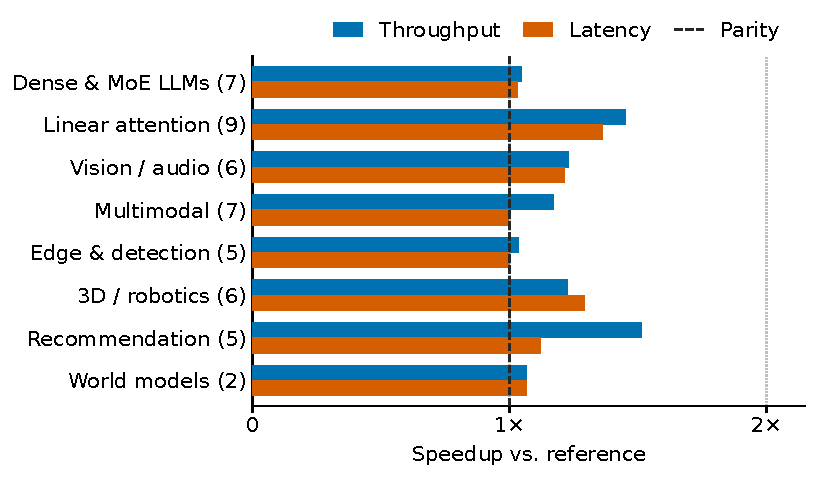
\includegraphics[width=0.7\linewidth]{figures/fastkernels/eval_e2e.pdf}
\caption{\textbf{Composition and reference performance of \FastKernels}: 47 end-to-end architectures across 8 categories (count in parentheses).
Each bar is the geometric-mean end-to-end speedup of \FastKernels over the production reference across the category's architectures (throughput and latency) on B200 (\Cref{fastkernels:sec:eval-results}).}
\label{fastkernels:fig:arch_pie}
\label{fastkernels:fig:eval-e2e}
\end{figure}

\subsection{Interface-Compatible Design}
\label{fastkernels:sec:interface}

A central design principle of \FastKernels is that optimized kernels should be deployable into existing production systems with minimal effort.
For each model architecture family, we identify the corresponding state-of-the-art production library (e.g., vLLM for LLMs, SGLang for serving) and design each task's interface---its \texttt{\_\_init\_\_} constructor signature and \texttt{forward} method---to closely match the corresponding module in that reference library.

A kernel optimized within \FastKernels can therefore be copied into vLLM, SGLang, or another production framework without interface refactoring.
Unlike FlashInfer-Bench's FIApply, which substitutes at the kernel dispatch level (an abstraction internal to FlashInfer), \FastKernels's compatibility operates at the \emph{module} level, the unit production frameworks compose.
\Cref{fastkernels:fig:interface} shows two representative examples, the Mamba-2 mixer and its gated RMSNorm, side by side with the corresponding vLLM modules.
The shared \texttt{\_\_init\_\_} and \texttt{forward} arguments make substitution a file swap: call sites need not change, and any residual differences are optional framework kwargs rather than a different compute interface.

\begin{figure}[tbp]
\noindent\textbf{Mamba-2 mixer.}

\noindent
\begin{minipage}[t]{0.48\linewidth}
\vspace{0pt}
\textbf{\FastKernels interface:}
\begin{lstlisting}[basicstyle=\ttfamily\scriptsize,columns=fullflexible,keepspaces=true,breaklines=true,showstringspaces=false,frame=single,aboveskip=2pt,belowskip=2pt]
class Mamba2Mixer(nn.Module):
  def __init__(self, hidden_size,
      ssm_state_size,
      conv_kernel_size,
      intermediate_size,
      use_conv_bias, use_bias,
      n_groups=1, num_heads=128,
      head_dim=64,
      rms_norm_eps=1e-5,
      activation="silu",
      use_rms_norm=True, ...):
    ...

  def forward(self, hidden_states):
    ...
\end{lstlisting}
\end{minipage}
\hfill
\begin{minipage}[t]{0.48\linewidth}
\vspace{0pt}
\textbf{vLLM interface:}
\begin{lstlisting}[basicstyle=\ttfamily\scriptsize,columns=fullflexible,keepspaces=true,breaklines=true,showstringspaces=false,frame=single,aboveskip=2pt,belowskip=2pt]
class MambaMixer2(nn.Module):
  def __init__(self, hidden_size,
      ssm_state_size,
      conv_kernel_size,
      intermediate_size,
      use_conv_bias, use_bias,
      n_groups=1, num_heads=128,
      head_dim=64,
      rms_norm_eps=1e-5,
      activation="silu",
      use_rms_norm=True, ...):
    ...

  def forward(self, hidden_states):
    ...
\end{lstlisting}
\end{minipage}

\medskip

\noindent\textbf{Mamba-2 gated RMSNorm.}

\noindent
\begin{minipage}[t]{0.48\linewidth}
\vspace{0pt}
\textbf{\FastKernels interface:}
\begin{lstlisting}[basicstyle=\ttfamily\scriptsize,columns=fullflexible,keepspaces=true,breaklines=true,showstringspaces=false,frame=single,aboveskip=2pt,belowskip=2pt]
class Mixer2RMSNormGated(
    nn.Module):
  def __init__(self,
      full_hidden_size,
      full_n_groups,
      use_rms_norm=True,
      eps=1e-6):
    ...

  def forward(self, x, gate):
    ...
\end{lstlisting}
\end{minipage}
\hfill
\begin{minipage}[t]{0.48\linewidth}
\vspace{0pt}
\textbf{vLLM interface:}
\begin{lstlisting}[basicstyle=\ttfamily\scriptsize,columns=fullflexible,keepspaces=true,breaklines=true,showstringspaces=false,frame=single,aboveskip=2pt,belowskip=2pt]
class Mixer2RMSNormGated(
    nn.Module):
  def __init__(self,
      full_hidden_size,
      full_n_groups,
      use_rms_norm=True,
      eps=1e-6):
    ...

  def forward(self, x, gate):
    ...
\end{lstlisting}
\end{minipage}
\caption{\textbf{Interface compatibility.} The \FastKernels task interfaces of the Mamba-2 mixer (top) and gated RMSNorm (bottom), next to the corresponding vLLM modules.}
\label{fastkernels:fig:interface}
\end{figure}

\subsection{Multi-GPU Communication Kernels}
\label{fastkernels:sec:multigpu}

Production inference at scale is almost always distributed, and its collectives and communication--computation overlaps materially affect end-to-end latency.
\FastKernels includes the communication path of its tensor-parallel models as tasks: the custom IPC all-reduce (L1); the tensor-parallel linear, embedding, and MoE layers that issue it (L2); and a decoder layer that fuses it with residual addition and RMSNorm (L3).
The all-reduce and row-parallel linear are benched in a real NCCL group of the capture's TP degree, and all of these operators run end to end inside models served at TP 2--8.
Dedicated benchmarks~\citep{commbench,parallelkernelbench} cover more communication patterns but score each program in isolation; \FastKernels places every collective in the schedule it shares with the model's compute kernels, where a kernel $1.5\times$ faster on one GPU can still slow the model.

\section{Benchmarking Stack}
\label{fastkernels:sec:benchmarking_tooling}

\FastKernels exposes one evaluation stack through two tiers, \emph{kernel-level} (\texttt{fastkernels bench}) and \emph{end-to-end} (\texttt{fastkernels eval}), each usable as a diagnostic tool or in leaderboard mode.
Both tiers operate on \emph{scenario sets} (\Cref{fastkernels:sec:scenarios}) and on the workloads captured from them (\Cref{fastkernels:sec:capture}); \Cref{fastkernels:sec:tiers} describes the tiers themselves and \Cref{fastkernels:sec:drift} how the production baselines they score against are versioned.

\subsection{Scenario Sets}
\label{fastkernels:sec:scenarios}

A scenario fixes a checkpoint, tensor-parallel degree, dtype, and workloads from public datasets for its modality (e.g., WildChat for LLMs, Parti-prompts for diffusion, COCO for detection).
Scenario sets are YAML tables shipped with \FastKernels; per-workload datasets, request counts, and sequence lengths are defined once in a workload registry, so every tier and every run of a set sees identical inputs.
Four sets ship with the benchmark:
\begin{itemize}[leftmargin=*, itemsep=1pt, topsep=2pt]
\item \textbf{full}: one scenario per architecture (47 scenarios, 184 workloads, TP 1--8; BF16, FP16, FP32, FP8, MXFP4, and NVFP4), and therefore every task. It is the set on which we validate the baselines against production references (\Cref{fastkernels:sec:eval-results}).
\item \textbf{default}: the 11 scenarios of \Cref{fastkernels:tab:default_scenarios} (48 workloads), on which all agent results are reported. It contains at least one model per category, which \textsc{MacroEval}'s per-family averaging requires, spans TP 1, 2, and 4 and BF16, FP16, FP8, and MXFP4 execution, and pairs throughput workloads (batched request mixes) with latency workloads (single requests or small fixed batches) for every model. Its B200 capture exercises 133 L1--L3 tasks (47 L1, 64 L2, 22 L3), which are the agents' targets; \texttt{oasis\_rollout}, a whole-model rollout driver rather than a kernel, is excluded from scoring, leaving 21 L3 targets.
\item \textbf{minimal}: Llama-3.1-8B with two workloads, a smoke test for the capture-to-bench pipeline.
\item \textbf{vllm\_only}: the 16 architectures whose reference is vLLM, used to compare vLLM releases for drift tracking (\Cref{fastkernels:sec:drift}).
\end{itemize}
Agents are scored on the default set rather than the full set because of cost: the long-horizon agents of \Cref{fastkernels:sec:eval-agents} spend 1{,}763--2{,}512 agent-hours each on the default set's 133 operators (\Cref{fastkernels:sec:eval-setup}), and the full set's architectures use more than twice as many L1--L3 tasks (337 versus 159 under the counting rule of \Cref{fastkernels:sec:coverage}, of which the default workloads invoke 133 on B200).

\begin{table}[t]
  \centering
  \caption{\textbf{The default scenario set.} Workloads are listed by name; their datasets and sizes are defined in the workload registry (\Cref{fastkernels:sec:eval-setup}).}
  \label{fastkernels:tab:default_scenarios}
  \scriptsize
  \setlength{\tabcolsep}{3pt}
  \begin{adjustbox}{max width=\linewidth}
  \begin{tabular}{@{}llcl>{\raggedright\arraybackslash}p{5.6cm}@{}}
  \toprule
  \textbf{Model} & \textbf{Category} & \textbf{TP} & \textbf{dtype} & \textbf{Workloads} \\
  \midrule
  Llama-3.1-8B-Instruct & Dense \& MoE LLMs & 1 & BF16 & mixed, long-context, single request, fixed batch 32 \\
  gpt-oss-120b & Dense \& MoE LLMs & 2 & MXFP4 & mixed, long-context, single request, fixed batch 32 \\
  Qwen3-Next-80B-A3B-Instruct & Linear Attention & 2 & BF16 & mixed, long-context, single request, fixed batch 32 \\
  Kimi-Linear-48B-A3B-Instruct & Linear Attention & 2 & BF16 & mixed, long-context, single request, fixed batch 32 \\
  GLA-2.7B & Linear Attention & 1 & BF16 & mixed, long-context, single request, fixed batch 32 \\
  FLUX.1-dev & Vision / Video / Audio & 1 & BF16 & 512 and 1024 px, batched and single image \\
  Qwen3-VL-235B-A22B-Instruct-FP8 & Multimodal & 4 & FP8 & text only, image, video, single image, single video \\
  YOLOv10n & Edge \& Detection & 1 & FP16 & COCO val, single image, batch 4 \\
  OpenFold3 & 3D / Robotics / Science & 1 & BF16 & four length buckets, batched and single \\
  BGE-M3 & Recommendation & 1 & FP16 & MLDR documents, single request, fixed batch 32 \\
  Oasis-500M & World Models & 1 & FP16 & four rollout / denoising settings, batch-1 latency \\
  \bottomrule
  \end{tabular}
  \end{adjustbox}
\end{table}

\subsection{Workload Capture and Case Selection}
\label{fastkernels:sec:capture}

The kernel tier does not benchmark synthetic shapes: it benchmarks the cases that the scenarios of a set actually produce, which \texttt{fastkernels capture} records by running each scenario end to end.

\paragraph{Instrumentation.}
\texttt{fastkernels capture <set>} loads each scenario into its own engine process (a TP-$N$ scenario claims $N$ GPUs; scenarios are packed onto the GPU pool and isolated so that a crash in one does not affect the others) and runs every listed workload on its real inputs.
Before the model is built, it wraps the constructor and \texttt{forward} of every \texttt{nn.Module} class under \texttt{tasks/baseline}.
A constructor call is recorded as a reconstructable \emph{recipe}: configuration dataclasses and enums with their field values, dtypes, tensor shapes, and references to other captured operators (e.g., the linear layers inside an attention block); runtime handles such as process groups are marked opaque.
A forward call is recorded as the shape, dtype, and, for non-contiguous tensors, stride of every tensor argument, together with the values of scalar arguments.
Shape capture stores no weights or activation values; golden inputs for data-dependent operators are recorded separately (below).

\paragraph{Deduplication.}
Each call is keyed by the canonical serialization of its record, and identical keys are merged into one \emph{variant} that keeps a call count.
Each forward variant also records which constructor variants built the instances it ran on, so the benchmark can rebuild exactly the module configuration that produced each shape.
Since every layer of a model and every decode step with the same batch composition produce the same key, the 12.4M L1--L3 forward calls of the default B200 capture reduce to 93.3K variants across its 48 per-workload reports, and to 87.7K distinct (constructor, forward) cases once merged across reports.
The distribution is long-tailed: half of the operators have at most seven distinct cases, while operators whose shapes follow the per-step token count (decode attention, RMSNorm, linear layers, embeddings) reach thousands.
For the few operators that read the global inference context inside \texttt{forward} (MLA attention), a coarse context summary (prefill or decode, and a power-of-two bucket of the number of prefill sequences) is folded into the key, which is enough to rebuild the code path without defeating deduplication.

\paragraph{Verification.}
Two independent checks run after every workload.
First, a forward pre-hook, registered separately from the wrappers, re-observes every operator call; its per-operator keys and counts must match the wrapper records.
Second, a mock continuous-batching and chunked-prefill scheduler, driven only by each request's real prompt and generated lengths, the engine's token and sequence budgets, and its KV-block pool, replays the serving schedule and predicts the per-step batch composition; the captured leading dimensions (token counts, sequence counts, batch sizes) must agree with it.
The replay does not model speculative decoding, so only the first check applies to EAGLE-3.

\paragraph{Case selection.}
\texttt{fastkernels bench} loads every report of a capture and deduplicates cases across reports by (constructor recipe, forward record).
When an operator has more than five distinct cases (the default budget), it keeps the smallest, median, and largest by total input elements and fills the remaining slots with the most frequently called cases, so the selection covers the size range rather than only the hot decode shape.
On the default B200 capture this yields 582 benchmarked cases over the 154 operator classes defined in the 133 target tasks.

\paragraph{Input materialization.}
Floating-point inputs are drawn from a standard normal (FP8 inputs are clamped normals cast to FP8) and masks are all ones.
Integer tensors are made valid for the call: cumulative sequence-length vectors are rebuilt as partitions consistent with the query and key token counts, token and position indices are bounded by the vocabulary size and maximum position, expert indices by the expert count, and slot mappings and block tables by the cache they index.
Captured non-contiguous layouts are reproduced with the recorded strides.
Baseline and candidate share randomly initialized weights; quantized weights (block-scaled FP8, NVFP4, MXFP4) are produced with the model's own quantization and weight-preparation routines, so kernels see the layouts they would see after checkpoint loading.
For data-dependent operators such as MoE dispatch, whose control flow depends on input values (\Cref{fastkernels:sec:eval-input-capture}), the kernel tier can instead replay golden inputs captured from real end-to-end executions, so that correctness and performance are measured on the tensors the model actually produces.
Cases whose inputs the baseline rejects, or whose baseline output is all zeros (so that a stub would pass), are skipped.
The all-reduce and row-parallel linear run in an NCCL group spawned with world size equal to the capture's TP degree, with every rank executing the same seeded cases.

\paragraph{Correctness and timing.}
Each case runs three rounds of fresh inputs, and an output passes when at least 99\% of its elements are within per-dtype tolerances ($\mathrm{atol},\mathrm{rtol}$ of $10^{-5},10^{-3}$ for FP32; $10^{-2},10^{-2}$ for FP16 and BF16; $0.125,0.125$ for FP8).
Timing uses CUDA events with 10 warm-up and 50 timed iterations, flushing the L2 cache and rotating input buffers between iterations, and reports the median.
Each operator runs in its own process, where the harness checks the identity of the timing primitive and of its own critical functions, background-thread counts, and output types, and reports any tampering as a reward hack.

\subsection{Case Study: Captured Inputs Matter for Data-Dependent Operators}
\label{fastkernels:sec:eval-input-capture}

\begin{figure}[t]
\centering
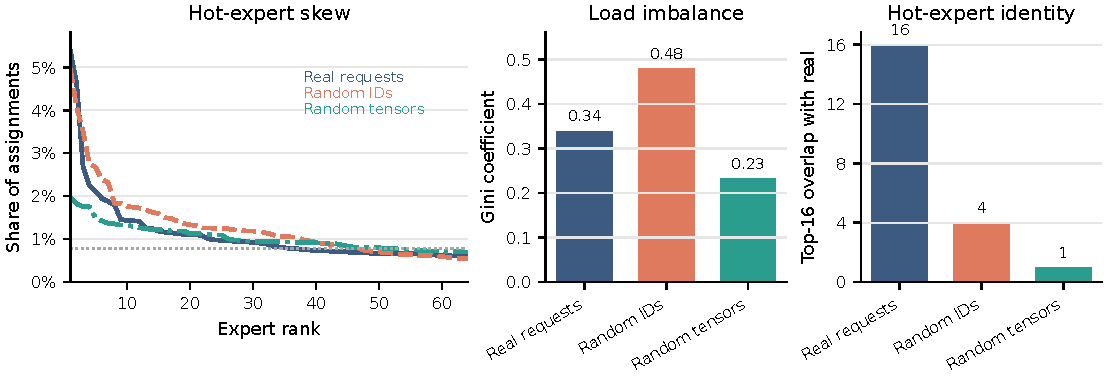
\includegraphics[width=0.7\textwidth]{figures/fastkernels/moe_input_capture.pdf}
\caption{\textbf{Input capture changes data-dependent execution.} First MoE layer of Qwen3-VL-30B-A3B-Instruct-FP8 (128 experts, top-8 routing) under three inputs: real WildChat requests, random token IDs (matched lengths), and random tensors injected at the gate. Random tensors look near-uniform; random tokens skew differently from real requests, with only 4 of the top-16 hot experts in common.}
\label{fastkernels:fig:moe-input-capture}
\end{figure}

Many production operators have data-dependent control flow---which experts, sparse blocks, cache slots, or communication paths execute is determined by the input.
We isolate this effect on a well-known case: the first MoE gate of Qwen3-VL-30B-A3B-Instruct-FP8 (\Cref{fastkernels:fig:moe-input-capture}). Random tensors yield a near-uniform gate (Gini $0.232$); random token IDs over-concentrate load and identify different hot experts from real WildChat requests (Gini $0.480$ vs.\ $0.339$; only $4 / 16$ shared hot experts).
\FastKernels's capture-and-replay path therefore rewards data-dependent kernels on the tensors production requests actually create, rather than on synthetic control flow: the kernel tier can replay golden inputs captured from real end-to-end executions (\Cref{fastkernels:sec:capture}), and the end-to-end tier runs real requests.

\subsection{Kernel-Level and End-to-End Tiers}
\label{fastkernels:sec:tiers}

\paragraph{Kernel-level tier.}
The kernel tier rebuilds each candidate next to its baseline from the captured recipe, shares weights, and compares outputs and runtimes on the selected cases, one operator per isolated process with reward-hack checks (\Cref{fastkernels:sec:capture}).
Values are synthesized from the captured shapes, with offsets, indices, and cache slots kept consistent with the call; for data-dependent operators such as MoE dispatch, \FastKernels additionally replays golden inputs captured from real end-to-end executions, ensuring that both correctness and performance are measured on the actual tensors encountered by the model (\Cref{fastkernels:sec:eval-input-capture}).

\paragraph{End-to-end tier.}
The end-to-end tier swaps a candidate set into full model executions on the production path and real requests, next to a baseline run and a noise run that calibrates correctness thresholds, and produces the \textsc{MacroEval} metrics (\Cref{fastkernels:sec:metrics}).
The kernel tier gives agents fast feedback; the end-to-end tier is the ground truth that the leaderboard reports.
Both tiers integrate with profilers, NVIDIA Nsight Compute (NCU) for kernel-level analysis and Nsight Systems (NSYS) for end-to-end traces, with LLM-based extraction of the main bottlenecks, and with MLflow for tracking kernel lineage across agent runs.

\paragraph{Leaderboard and submission portal.}
\FastKernels hosts a public leaderboard that ranks agent--mode entries by their \textsc{MacroEval} score (\Cref{fastkernels:sec:eval-e2e}), and a submission portal through which an agent is submitted as a repository of candidate files and scored with the same two-tier harness.

\subsection{Baseline Versioning and Drift}
\label{fastkernels:sec:drift}

Production kernels are a moving target, so \FastKernels is versioned: each release pins the exact revision of every reference library (vLLM, FlashInfer, FLA, diffusers, \dots) per target GPU, and the results in this chapter use vLLM~0.26.0 (released 2026-07-25).
A speedup over a \FastKernels baseline is therefore a speedup over production at that release.
To track drift, \FastKernels ships a daily CI job (\texttt{scripts/baseline\_drift.sh}): whenever a new vLLM release appears, it re-benchmarks only the reference models under that release on each pinned GPU type, in isolated environments with one job per node, and computes per-family drift coefficients (per-model geometric mean over workloads, models weighted equally within a family).
Dividing a speedup measured against the pinned baseline by the family coefficient estimates the speedup against the newer release; when any family moves by more than 10\%, a re-release with re-pinned references is prepared.

To estimate the cadence this implies, we ran the same measurement over the 127 days between vLLM~0.18.0 (2026-03-20) and 0.26.0 on 8$\times$H200 and 8$\times$B200, on the 13 reference models both releases serve, with identical workloads (\Cref{fastkernels:tab:drift}).
The median model moved by only $1.03\times$ (throughput) and $1.01\times$ (latency) on H200, and by $1.07\times$ and $1.09\times$ on B200.
Drift is concentrated rather than uniform: one family crossed the 10\% threshold on H200 (linear attention and SSMs, $1.15\times$ throughput) and two on B200, where the LLM family is dominated by gpt-oss-120b's MXFP4 path maturing on Blackwell ($2.8\times$, against $1.04\times$ on H200).
Newer releases are not uniformly faster: Qwen3-VL-235B-FP8 lost throughput on both GPUs ($0.83\times$ and $0.87\times$).
This implies a re-release at least every four months, sooner on newer hardware whose support for new number formats is still maturing---comparable to the cadence at which any benchmark that stays current must add newly released architectures.

\begin{table}[t]
  \centering
  \caption{\textbf{Reference drift from vLLM~0.18.0 to 0.26.0} (127 days), as computed by the baseline-drift CI job: speedup of the newer release (${>}1$: faster), per-model geometric mean over workloads, models weighted equally within a family.
  Latencies are 5-iteration medians (${<}1\%$ spread); throughput is one timed pass per workload, which three repeated runs per release of Qwen3-VL-235B-FP8 place within 1.5\%.
  On B200, six models needed \texttt{nvidia-cutlass-dsl==4.5.3} to import under vLLM~0.18.0.}
  \label{fastkernels:tab:drift}
  \small
\begin{tabular}{@{}lr rr rr@{}}
\toprule
 & & \multicolumn{2}{c}{\textbf{H200}} & \multicolumn{2}{c}{\textbf{B200}} \\
\cmidrule(lr){3-4}\cmidrule(lr){5-6}
Model family & $n$ & Thr. & Lat. & Thr. & Lat. \\
\midrule
LLM (dense + MoE) & 3 & 1.09$\times$ & 1.08$\times$ & 1.44$\times$ & 1.37$\times$ \\
Linear attention / SSM / hybrid & 5 & 1.15$\times$ & 1.03$\times$ & 1.14$\times$ & 1.18$\times$ \\
Multimodal / VLM & 4 & 0.98$\times$ & 1.05$\times$ & 1.01$\times$ & 1.07$\times$ \\
Audio & 1 & 1.02$\times$ & 1.02$\times$ & 1.02$\times$ & 1.07$\times$ \\
\midrule
Median model & 13 & 1.03$\times$ & 1.01$\times$ & 1.07$\times$ & 1.09$\times$ \\
\bottomrule
\end{tabular}
\end{table}

\section{\textsc{MacroEval}: Cross-Architecture Metrics}
\label{fastkernels:sec:metrics}

\FastKernels evaluates candidate kernels by substituting them into end-to-end model executions and comparing each run with a reference run that uses the production baseline kernels.
The key challenge is that model families expose different correctness signals---tokens, embeddings, labels, rankings, trajectories, audio, or video---and different throughput--latency tradeoffs.
\textsc{MacroEval} addresses this by calibrating architecture-specific correctness to a common $[0,1]$ scale, measuring end-to-end speedup, and macro-averaging across families so no single architecture dominates the leaderboard.

\paragraph{Benchmark indexing.}
Let $f \in \mathcal{F}$ index architecture families, such as LLMs, diffusion models, vision models, speech and audio models, retrieval and recommender models, and robotics or world models.
For family $f$, let $i \in B_f$ index benchmark items, and let $r \in R_i$ index requests, prompts, seeds, or input instances for item $i$.
We write $y_{\mathrm{ref},i,r}$ and $y_{\mathrm{cand},i,r}$ for the reference and candidate outputs, and $T_{\mathrm{ref},i}$ and $T_{\mathrm{cand},i}$ for their measured runtimes.

\paragraph{Calibrated correctness.}
Raw output discrepancies are inherently architecture-dependent: teacher-forced top-1 disagreement with the reference tokens for autoregressive models (free-running greedy outputs diverge even between two correct runs, e.g.\ after a fresh compile), embedding or output distance for encoders and diffusion models, IoU discrepancy for detection or segmentation, WER/CER deltas for speech, ranking disagreement for retrieval, and trajectory error for robotics.
For each request, \FastKernels therefore computes a discrepancy $d_{i,r} = D_f(y_{\mathrm{cand},i,r}, y_{\mathrm{ref},i,r})$, with $D_f$ chosen for the output type of family $f$, and maps it to a calibrated correctness score in $[0,1]$:
\begin{equation}
C_{i,r} =
\begin{cases}
1, & d_{i,r} \le g_i, \\
\frac{f_i - d_{i,r}}{f_i - g_i}, & g_i < d_{i,r} < f_i, \\
0, & d_{i,r} \ge f_i.
\end{cases}
\end{equation}
Here $g_i$ is the threshold below which the candidate is indistinguishable from the reference, and $f_i$ is the threshold above which the output is incorrect or unusable.
Thresholds are fixed before evaluation. $g_i$ is calibrated per model from reference-vs-reference nondeterminism: a \emph{noise run} repeats the production reference in a fresh process with a cold compile cache (re-making every compilation and autotuning choice, as a candidate run does), and $g_i$ is the 95th percentile of its per-sample discrepancy against the reference, with a floor of $10^{-3}$.
The one exception is OpenFold3, which runs eagerly and deterministically, so that its noise run reproduces the reference bit for bit while its diffusion sampling amplifies any numerical change; its $g_i$ therefore comes from a calibration run that instead disables cuBLAS reduced-precision BF16 reductions, a benign numerical change.
We set $f_i = 0.5$ for every family---a candidate at least half as far from the reference as an unrelated output receives no credit---and $\tau_i = 0.9$; \Cref{fastkernels:tab:e2e-sensitivity} shows that the ranking is unchanged when $g_i$ and $f_i$ are halved or doubled.

Correctness is averaged over requests, then over items within each family, then over families:
\begin{equation}
C_i = \frac{1}{|R_i|}\sum_{r \in R_i} C_{i,r},
\qquad
C_f = \frac{1}{|B_f|}\sum_{i \in B_f} C_i,
\qquad
C_{\mathrm{macro}} = \frac{1}{|\mathcal{F}|}\sum_{f \in \mathcal{F}} C_f.
\end{equation}
This macro-family weighting gives each architecture family equal influence and prevents overrepresented families, such as LLMs, from dominating the correctness axis.

\paragraph{Validity and coverage.}
Although calibrated correctness is continuous, deployment requires a hard validity decision for each benchmark item.
We define $\operatorname{valid}_i = \mathbf{1}(C_i \ge \tau_i)$ for a pre-specified item or family threshold $\tau_i$.
Items are invalid if they crash, hang, trigger shape or type errors, access memory illegally, produce NaNs, or fall below the correctness threshold.
We report both item-level coverage and macro-family coverage:
\begin{equation}
\mathrm{Coverage} = \frac{1}{N}\sum_i \operatorname{valid}_i,
\qquad
\mathrm{Coverage}_{\mathrm{macro}} =
\frac{1}{|\mathcal{F}|}\sum_{f \in \mathcal{F}}
\frac{1}{|B_f|}\sum_{i \in B_f}\operatorname{valid}_i.
\end{equation}
Macro-coverage is the preferred statistic when architecture balance matters.

\paragraph{Throughput--latency speedup.}
For valid items (invalid items receive no speedup credit), performance is measured against the production reference with a geometric blend of throughput and latency speedups:
\begin{equation}
s_i =
\left(s_i^{\mathrm{thr}}\right)^{\lambda}
\left(s_i^{\mathrm{lat}}\right)^{1-\lambda},
\qquad
s_i^{\mathrm{thr}} =
\frac{\mathrm{Throughput}_{\mathrm{cand},i}}
     {\mathrm{Throughput}_{\mathrm{ref},i}},
\qquad
s_i^{\mathrm{lat}} =
\frac{\mathrm{Latency}_{\mathrm{ref},i}}
     {\mathrm{Latency}_{\mathrm{cand},i}}.
\end{equation}
The default $\lambda = 0.5$ is neutral: an optimization that improves throughput while equivalently degrading latency receives no net credit, since such gains are workload-dependent tradeoffs rather than universal improvements; users may pre-specify a different $\lambda$.
Because speedups are multiplicative, \FastKernels aggregates the blended speedups with geometric means.
For each family, let $B_f^{\mathrm{valid}} = \{i \in B_f : \operatorname{valid}_i = 1\}$.
The family-level and macro-geometric speedups are
\begin{equation}
S_f =
\exp\left(
\frac{1}{|B_f^{\mathrm{valid}}|}
\sum_{i \in B_f^{\mathrm{valid}}}\log s_i
\right),
\qquad
S_{\mathrm{macro}} =
\exp\left(
\frac{1}{|\mathcal{F}_{\mathrm{valid}}|}
\sum_{f \in \mathcal{F}_{\mathrm{valid}}}\log S_f
\right),
\end{equation}
where $\mathcal{F}_{\mathrm{valid}}$ contains families with at least one valid item.
A family with no valid item is excluded from speedup aggregation, so incorrect kernels earn no performance credit, and the failure is penalized through macro-coverage instead.

\paragraph{Leaderboard.}
The leaderboard reports $S_{\mathrm{macro}}$, $C_{\mathrm{macro}}$, and $\mathrm{Coverage}_{\mathrm{macro}}$ separately, so users can rank agents by whichever their deployment prioritizes.
As the default single ranking, \FastKernels uses their product $\mathrm{Score}_{\mathrm{default}} = S_{\mathrm{macro}} \cdot C_{\mathrm{macro}} \cdot \mathrm{Coverage}_{\mathrm{macro}}$, which rewards agents that are simultaneously fast, correct, and broadly applicable, and it also reports throughput-only ($\lambda{=}1$) and latency-only ($\lambda{=}0$) rankings for batched and interactive deployments.
All speedups are measured empirically against the reference, without speed-of-light or roofline bounds.

\section{Evaluation}
\label{fastkernels:sec:evaluation}

The evaluation has three parts: \Cref{fastkernels:sec:eval-setup} describes the hardware, workloads, and agents; \Cref{fastkernels:sec:eval-results} evaluates the \emph{benchmark itself}, checking that its baselines match each family's production framework so that speedups over them are meaningful; and \Cref{fastkernels:sec:eval-agents,fastkernels:sec:eval-e2e} evaluate \emph{kernel agents} on the default set, at the kernel level and end to end.

\subsection{Experimental Setup}
\label{fastkernels:sec:eval-setup}

\paragraph{Hardware.}
End-to-end L4 validation results (\Cref{fastkernels:sec:eval-results}) are measured on a NVIDIA DGX B200 box with 8x NVIDIA B200 SXM GPUs, 180 GB HBM3e each (1.44 TB total), interconnected via 5th-gen NVLink/NVSwitch.
Single-GPU experiments use one GPU; multi-GPU experiments use up to $8\times$B200 (tensor-parallel degree matching the production reference: e.g.\ TP=2 Mixtral/GPT-OSS, TP=8 GLM-5.2).
L1--L3 agent captures (\Cref{fastkernels:sec:eval-agents}) use the same B200 nodes.
The Hopper validation repeats the same L4 scenario table on a node with 8x NVIDIA H200 SXM GPUs, 141 GB HBM3e each, using the same tensor-parallel degrees; GLM-5.2 is not run there because its NVFP4 kernels require Blackwell.

\paragraph{Serving benchmark.}
Autoregressive L4 throughput uses a mixed-length request mix and a long-context mix against the production server (vLLM, SGLang, or FLA); latency uses single-request (batch 1) and fixed-batch-32 decoding.
Each latency measurement is the median of 5 iterations.
Non-AR models use family-specific public workloads (Parti-prompts, SEED-TTS-Eval, LibriSpeech, COCO val, Food101, MS MARCO, ALOHA, etc.), as defined in the workload registry of \Cref{fastkernels:sec:scenarios}.
In the end-to-end agent evaluation (\Cref{fastkernels:sec:eval-e2e}), Qwen3-VL-235B uses 200 requests per throughput workload and 32 correctness samples; GLA and OpenFold3 were re-run on cloud B200 nodes after a harness fix, and Codex's sets on a separate B200 node (its Llama baseline throughput is within 0.02\% of the other node's).
Every set's speedups and discrepancies are relative to the baseline measured in the same run.

\paragraph{Agent selection.}
We chose agents to cover the three lines of work that currently produce the strongest kernels.
From the KernelBench ecosystem we run Dr.~Kernel~\citep{drkernel}, an RL-trained model and one of its most recent agents; of the others we tried, KernelAgent~\citep{kernelagent} did not reproduce its reported results in our setting, and the rest assume KernelBench's single-file tasks with a self-contained reference and cannot load production-shaped modules that require configuration objects, KV-cache wrappers, packed quantized weights, or a distributed context.
From the MLSys 2026 FlashInfer AI Kernel Generation Contest~\citep{mlsys26contest}, whose tasks were drawn from production LLM workloads and scored against FlashInfer's expert kernels, we run KDA~\citep{kda}, whose full-agent entry placed first on MoE, second on DSA, and third on GDN, and AKO~\citep{ako} (its AKO4X harness was adapted by the GEMM People entry, which placed second on MoE), whose release reports beating the FlashInfer expert kernels on 9 of 10 operator families on B200.
Finally, we run Claude Code and Codex~\citep{codex} directly, with no harness.
Because KDA and AKO drive the same Claude model as our Claude Code runs (KDA adds a GPT reviewer), comparing them with Claude Code isolates the contribution of the harness.

\paragraph{Agent configurations.}
\Cref{fastkernels:tab:agent-config} summarizes how each agent was run.
All agents receive the same task: the baseline module, its captured cases, and \texttt{fastkernels bench} on a GPU that is leased only while they benchmark or profile.
A candidate becomes a \emph{winner} only if every non-skipped case passes and its geometric-mean speedup is at least $1\times$; an unchanged baseline that passes counts as correct at $1\times$ but not as a fast$_1$ win.
The independent campaign optimizes all 133 operators in standalone mode; the sequential campaign regenerates the 86 L2 and L3 operators on top of the frozen lower-level winners.

\begin{table}[t]
  \centering
  \caption{\textbf{Agent configurations.} \emph{Cap}: hang cap on one agent session (the candidate is kept on timeout), not a target budget.}
  \label{fastkernels:tab:agent-config}
  \scriptsize
  \setlength{\tabcolsep}{3pt}
  \begin{adjustbox}{max width=\linewidth}
  \begin{tabular}{@{}l>{\raggedright\arraybackslash}p{3.4cm}>{\raggedright\arraybackslash}p{6.2cm}l@{}}
  \toprule
  \textbf{Agent} & \textbf{Model(s)} & \textbf{Loop per operator} & \textbf{Cap} \\
  \midrule
  Dr.~Kernel & released \texttt{drkernel-14b} & 8 samples $\times$ 3 generate--execute--feedback turns (temperature 1.0, top-$p$ 0.95) & --- \\
  Claude Code & Claude Opus 5 (1M context, high effort) & one session with the default tools & 5\,h \\
  Codex & GPT-5.6 sol (high) & one session, same prompt as Claude Code & 5\,h \\
  KDA & Claude Opus 5 (draft, plan, implement); GPT-5.6 sol (review) & one planning cycle, then two implement--review rounds, with KernelWiki and Nsight Compute skills & 6\,h \\
  AKO & Claude Opus 5 (master and sub-agents) & two master-directed rounds, each a fresh sub-agent rewriting the kernel along one direction; improving kernels are archived & 5\,h/round \\
  \bottomrule
  \end{tabular}
  \end{adjustbox}
\end{table}

\paragraph{Budget and the number of agents.}
\Cref{fastkernels:tab:agent-cost} reports what each agent spent: 6{,}914 agent-hours and 41.9B tokens (266M output tokens) in total, of which Claude Code, KDA, and AKO account for 1{,}763, 2{,}512, and 2{,}234 agent-hours, with a median of 6--12 hours per operator.
These are the budgets at which such agents are used in practice: the MLSys 2026 contest gave teams 13 weeks, from the release of the starter kit (January 22) to the kernel deadline (April 24), to optimize five kernels~\citep{mlsys26contest}.
A leaderboard that samples many models for a few turns per task is far cheaper per entry, but it measures a different system than the long-horizon agents practitioners deploy, and the ranking of those agents is what \FastKernels is meant to report; we therefore evaluate fewer agents than single-turn leaderboards.
Each additional long-horizon agent costs about 2{,}000 agent-hours and 8--22B tokens on the default set.
Codex is the exception worth noting: its kernel-level results are comparable to the Claude-based agents' at 321 agent-hours.
\FastKernels imposes no structure on the agent, so any agent that writes candidate files can be scored with the same harness.

\begin{table}[t]
  \centering
  \caption{\textbf{Agent cost per campaign} (133 operators independently, 86 regenerated sequentially).
  \emph{Agent-hours}: sum over operators of each operator's wall-clock generation time, including relaunches; operators run in parallel, so this is not campaign wall-clock time.
  \emph{Tokens} as reported by each agent's CLI or API: input, output, and cached (re-read) context; output includes reasoning tokens.
  Dr.~Kernel runs a local model without prompt caching; KDA counts both its Claude and Codex sessions.}
  \label{fastkernels:tab:agent-cost}
  \small
  \setlength{\tabcolsep}{4pt}
\begin{tabular}{@{}ll r rr rrr@{}}
\toprule
 & & & \multicolumn{2}{c}{\textbf{Agent-hours}} & \multicolumn{3}{c}{\textbf{Tokens}} \\
\cmidrule(lr){4-5}\cmidrule(lr){6-8}
Agent & Campaign & Ops & Total & Median/op & Total (B) & Output (M) & Cached (\%) \\
\midrule
\multirow{2}{*}{Dr.~Kernel} & Independent & 133 & 53 & 0.26 & 0.03 & 10.4 & --- \\
 & Sequential & 86 & 32 & 0.34 & 0.02 & 8.0 & --- \\
\midrule
\multirow{2}{*}{Claude Code} & Independent & 133 & 1,171 & 7.27 & 4.35 & 31.4 & 97 \\
 & Sequential & 86 & 592 & 6.06 & 3.58 & 22.5 & 97 \\
\midrule
\multirow{2}{*}{KDA} & Independent & 133 & 1,751 & 12.33 & 12.31 & 62.8 & 96 \\
 & Sequential & 86 & 762 & 8.22 & 9.48 & 42.2 & 97 \\
\midrule
\multirow{2}{*}{AKO} & Independent & 133 & 1,421 & 9.43 & 5.47 & 47.4 & 97 \\
 & Sequential & 86 & 813 & 8.70 & 4.86 & 35.3 & 97 \\
\midrule
\multirow{2}{*}{Codex} & Independent & 133 & 253 & 1.86 & 1.02 & 4.0 & 98 \\
 & Sequential & 86 & 67 & 0.71 & 0.74 & 2.4 & 98 \\
\bottomrule
\end{tabular}
\end{table}

\paragraph{Evolutionary search.}
We omit evolutionary search.
AlphaEvolve~\citep{alphaevolve} and KernelEvolve~\citep{kernelevolve} are not publicly available.
OpenEvolve~\citep{openevolve} is, and was the organizers' agent baseline in the MLSys 2026 contest, but evolutionary frameworks evaluate a population of candidates in every generation, and on \FastKernels each evaluation compiles a kernel and benchmarks it on its production-shaped cases (for collectives, on a full tensor-parallel group); their cost per operator therefore scales with population size times the number of generations, on top of the LLM calls that produce each candidate, which puts a 133-operator campaign beyond our budget.
The AKO authors also report that, during the contest, search-based methods performed far worse than letting a coding agent optimize kernels directly~\citep{ako}.

\subsection{Benchmark Validation: Baselines vs.\ Production Frameworks}
\label{fastkernels:sec:eval-results}

On the full set, we benchmark every architecture's end-to-end performance (throughput and latency on real workloads) and the correctness of each L1--L4 task against the state-of-the-art production framework for its family (e.g., vLLM for LLMs, SGLang for serving, diffusers for SDXL, FLA for linear-attention recurrences, timm for vision encoders).
\Cref{fastkernels:fig:eval-e2e} reports the category-level geometric means on B200: gains concentrate in linear attention ($1.45\times$ throughput) and recommendation ($1.51\times$), and the other categories sit near parity.
References are pinned per release and GPU (vLLM~0.26.0 here); a daily CI job tracks their drift, 1--9\% for the median model over the four months before our pin (\Cref{fastkernels:sec:drift}).

Per architecture, the validation records the production reference, the public workload mix, the geometric mean of throughput and latency speedups over that mix, and an alignment metric against the reference (mean prefix-match length and exact-match rate for autoregressive models; cosine similarity, top-1 agreement, box/label agreement, or pass flags otherwise).
On B200, all 47 architectures run, and every architecture but two passes alignment: DLRMv2 reports a degenerate cosine against TorchRec on its checkpoint (with a maximum absolute difference of 0), and PointTransformerV3 sits just below threshold at feature cosine $0.986$.
The largest gains come from architectures whose production reference leaves performance on the table (Pi0 $3.1\times$ throughput, RetNet $3.4\times$, ColBERTv2 $3.1\times$, BGE-M3 $2.4\times$, CosyVoice3 $2.3\times$, Mamba $2.1\times$), whereas dense and MoE LLM serving against vLLM and SGLang stays within a few percent of parity in both directions.
Repeating the run on $8\times$H200 (46 architectures; GLM-5.2 is Blackwell-only) gives the same picture: the throughput geomean is $1.19\times$ on H200 versus $1.22\times$ on B200, the latency geomean is $1.15\times$ on both, the four largest H200 throughput gains (ColBERTv2, RetNet, Pi0, CosyVoice3) are also among the five largest on B200, and LLM serving stays at parity ($0.99\times$); the largest drops relative to B200 are Mamba ($2.10\times \to 1.08\times$) and BGE-M3 ($2.35\times \to 1.37\times$), and YOLOv10 fails alignment on H200, so its speedups there are not like-for-like.
We refer the reader to the \FastKernels paper~\cite{fastkernels} for the per-architecture B200 and H200 tables and speedup breakdowns.

\subsection{Agent Evaluation: Kernel-Level Results}
\label{fastkernels:sec:eval-agents}

\paragraph{Agents and modes.}
We evaluate the five agents of \Cref{fastkernels:sec:eval-setup}: Dr.~Kernel, an RL-trained kernel model from the KernelBench ecosystem; KDA and AKO, long-horizon harnesses behind winning MLSys 2026 FlashInfer contest entries; and Claude Code and Codex, the coding agents these harnesses build on.
Their campaigns total 6{,}900 agent-hours and 42B tokens (\Cref{fastkernels:tab:agent-cost}).
Each agent optimizes every L1--L3 operator captured from the default set on B200 (47 L1, 64 L2, and 21 L3 targets) against the human-expert kernels that production frameworks ship.
L4 tasks are full models, so benchmarking them is the end-to-end evaluation of \Cref{fastkernels:sec:eval-e2e}.
We bench L1--L3 in three modes:
\emph{independent} (each operator generated and benched in isolation, over production lower-level kernels),
\emph{composed} (the independent winners---correct, geomean speedup $\geq 1\times$---activated together, so higher-level kernels run on the agent's own lower-level winners), and
\emph{sequential} (L2 and L3 regenerated on top of the frozen lower-level winners, benched composed).

\paragraph{Results.}
Four agents reach geomean speedups of $1.6$--$6.6\times$ over the production kernels (\Cref{fastkernels:tab:kernel-levels}), but composition erodes them (\Cref{fastkernels:tab:kernel-composition}): once their children are also agent-generated, 26 of the agents' 71 L3 winners (37\%) fail correctness (13 of 18 for Codex), the surviving L3 winners of KDA and AKO lose 12--14\% of their speedup, and individual modules lose up to 76\% (Claude Code's \texttt{yolov10\_backbone}, $30.3\times \to 7.2\times$).
Sequential generation makes this an optimization target: it yields 80 correct L3 winners across agents instead of 45 composed, and the sequential L3 kernels of AKO and Codex are $1.48\times$ and $1.35\times$ faster than their composed independent ones.
\Cref{fastkernels:fig:kernel-fastp} extends the fast$_1$ and fast$_2$ columns of \Cref{fastkernels:tab:kernel-levels} to every speedup threshold $p$ for the independent mode: the curves separate the agents mostly at L2 and L3, where the long-horizon harnesses keep a large share of targets above $2\times$, while Dr.~Kernel's share decays quickly past parity at every level.

\begin{table}[t]
  \centering
  \caption{\textbf{Kernel agents on \FastKernels (B200, default set).}
  \emph{Corr.}: operators correct on every benchmarked case; \emph{Geo.}: geomean speedup over correct operators; fast$_p$: correct and more than $p\times$ faster than production (\Cref{fastkernels:fig:kernel-fastp}).
  Composed and sequential rows contain winners only.}
  \label{fastkernels:tab:kernel-levels}
  \small
  \setlength{\tabcolsep}{3pt}
  \begin{adjustbox}{max width=\linewidth}
\begin{tabular}{@{}llrrrrrrrrrrrr@{}}
\toprule
 & & \multicolumn{4}{c}{\textbf{L1} (47 targets)} & \multicolumn{4}{c}{\textbf{L2} (64 targets)} & \multicolumn{4}{c}{\textbf{L3} (21 targets)} \\
\cmidrule(lr){3-6}\cmidrule(lr){7-10}\cmidrule(lr){11-14}
Agent & Mode & Corr. & Geo. & fast$_{1}$ & fast$_{2}$ & Corr. & Geo. & fast$_{1}$ & fast$_{2}$ & Corr. & Geo. & fast$_{1}$ & fast$_{2}$ \\
\midrule
\multirow{3}{*}{Dr.~Kernel} & Independent & 31 & 0.93$\times$ & 18 & 1 & 18 & 0.59$\times$ & 5 & 0 & 4 & 0.97$\times$ & 1 & 0 \\
 & Composed & 18 & 1.29$\times$ & 18 & 1 & 5 & 1.07$\times$ & 4 & 0 & 1 & 1.03$\times$ & 1 & 0 \\
 & Sequential & 18 & 1.29$\times$ & 18 & 1 & 5 & 1.40$\times$ & 5 & 0 & 2 & 1.16$\times$ & 2 & 0 \\
\midrule
\multirow{3}{*}{Claude Code} & Independent & 47 & 1.81$\times$ & 42 & 10 & 64 & 2.66$\times$ & 56 & 37 & 20 & 4.74$\times$ & 19 & 16 \\
 & Composed & 42 & 1.79$\times$ & 40 & 10 & 54 & 3.52$\times$ & 54 & 36 & 14 & 6.28$\times$ & 14 & 12 \\
 & Sequential & 42 & 1.76$\times$ & 40 & 10 & 57 & 3.21$\times$ & 57 & 37 & 20 & 4.50$\times$ & 20 & 15 \\
\midrule
\multirow{3}{*}{KDA} & Independent & 47 & 1.64$\times$ & 42 & 8 & 63 & 2.56$\times$ & 61 & 37 & 20 & 3.05$\times$ & 18 & 14 \\
 & Composed & 43 & 1.69$\times$ & 40 & 9 & 51 & 2.62$\times$ & 51 & 31 & 11 & 3.45$\times$ & 11 & 9 \\
 & Sequential & 43 & 1.68$\times$ & 40 & 8 & 57 & 2.30$\times$ & 57 & 30 & 20 & 2.86$\times$ & 20 & 14 \\
\midrule
\multirow{3}{*}{AKO} & Independent & 45 & 1.84$\times$ & 44 & 11 & 64 & 3.35$\times$ & 64 & 41 & 18 & 6.48$\times$ & 18 & 17 \\
 & Composed & 45 & 1.87$\times$ & 44 & 11 & 60 & 3.54$\times$ & 60 & 43 & 14 & 6.59$\times$ & 14 & 13 \\
 & Sequential & 45 & 1.86$\times$ & 44 & 11 & 59 & 3.51$\times$ & 59 & 40 & 20 & 6.55$\times$ & 20 & 17 \\
\midrule
\multirow{3}{*}{Codex} & Independent & 47 & 1.62$\times$ & 40 & 9 & 64 & 2.87$\times$ & 60 & 39 & 19 & 2.92$\times$ & 18 & 12 \\
 & Composed & 41 & 1.76$\times$ & 40 & 9 & 47 & 3.52$\times$ & 45 & 33 & 5 & 5.79$\times$ & 5 & 4 \\
 & Sequential & 41 & 1.75$\times$ & 38 & 9 & 56 & 2.90$\times$ & 56 & 34 & 18 & 3.95$\times$ & 18 & 11 \\
\bottomrule
\end{tabular}
  \end{adjustbox}
\end{table}

\begin{table}[t]
  \centering
  \caption{\textbf{Composition effect and sequential generation}, over operators correct in both modes ($n$).
  \emph{Ratio}: geometric mean of the per-operator speedup ratio (composed / independent, or sequential / composed).
  \emph{Broke}: independent winners that fail correctness once composed.}
  \label{fastkernels:tab:kernel-composition}
  \small
  \setlength{\tabcolsep}{3pt}
\begin{tabular}{@{}l rrr rrr rr rr@{}}
\toprule
 & \multicolumn{6}{c}{\makecell{\textbf{Composition effect}\\(Independent $\to$ Composed)}} & \multicolumn{4}{c}{\makecell{\textbf{Sequential}\\(Composed $\to$ Seq.)}} \\
\cmidrule(lr){2-7}\cmidrule(lr){8-11}
 & \multicolumn{3}{c}{L2} & \multicolumn{3}{c}{L3} & \multicolumn{2}{c}{L2} & \multicolumn{2}{c}{L3} \\
\cmidrule(lr){2-4}\cmidrule(lr){5-7}\cmidrule(lr){8-9}\cmidrule(lr){10-11}
Agent & $n$ & Ratio & Broke & $n$ & Ratio & Broke & $n$ & Ratio & $n$ & Ratio \\
\midrule
Dr.~Kernel & 5 & 0.99$\times$ & 0 & 1 & 1.00$\times$ & 0 & 1 & 1.78$\times$ & 0 & --- \\
Claude Code & 54 & 1.09$\times$ & 2 & 14 & 0.99$\times$ & 4 & 50 & 0.99$\times$ & 14 & 0.97$\times$ \\
KDA & 51 & 0.98$\times$ & 10 & 11 & 0.88$\times$ & 6 & 47 & 0.90$\times$ & 11 & 1.07$\times$ \\
AKO & 60 & 1.00$\times$ & 4 & 14 & 0.86$\times$ & 3 & 55 & 1.05$\times$ & 14 & 1.48$\times$ \\
Codex & 47 & 0.97$\times$ & 13 & 5 & 1.04$\times$ & 13 & 43 & 0.94$\times$ & 5 & 1.35$\times$ \\
\bottomrule
\end{tabular}
\end{table}

\begin{figure}[t]
  \centering
  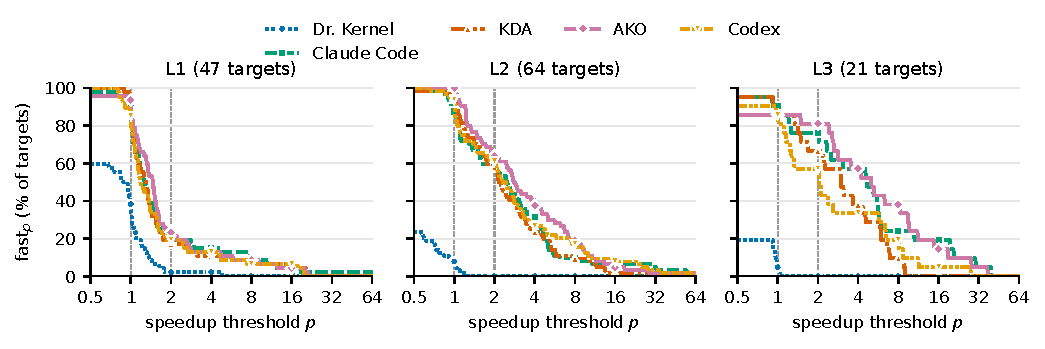
\includegraphics[width=\linewidth]{figures/fastkernels/kernel_fastp.pdf}
  \caption{\textbf{fast$_p$ by level (independent mode).} Share of targets whose kernel is correct and more than $p\times$ faster than the production baseline; the value at the left edge approaches the share of correct kernels. Dashed lines mark $p=1$ and $p=2$.}
  \label{fastkernels:fig:kernel-fastp}
\end{figure}

\subsection{Agent Evaluation: End-to-End Leaderboard}
\label{fastkernels:sec:eval-e2e}

We deploy each agent's independent and sequential winner sets into the 11 default models (each receiving the kernels it instantiates) and run their real workloads on the production path, next to a baseline run and a noise run (\Cref{fastkernels:sec:metrics}).
If a set crashes the model or grossly corrupts its outputs, the offending kernel (named in the traceback, else found by bisection) is dropped and the model re-run; the first subset that runs correctly is the agent's \emph{deployable subset}, timed on the full workloads.
\Cref{fastkernels:tab:e2e-macroeval} scores both the full winner sets as-is (\emph{all winners}) and the deployable subsets, and \Cref{fastkernels:tab:e2e-drops} counts the kernels each set requests and keeps across models and why kernels were dropped.
Per model, KDA's sets reach a deployable subset on all 11 models in both modes, whereas Dr.~Kernel, Claude Code, AKO, and Codex fail to converge to one within the attempt budget on 3, 8, 5, and 8 of their 22 (model, set) deployments, respectively; we refer the reader to the \FastKernels paper~\cite{fastkernels} for the per-model outcomes, speedups, and discrepancies of every agent set.

\begin{table}[t]
  \centering
  \caption{\textbf{End-to-end \textsc{MacroEval} leaderboard on the default set (B200).} \emph{Rank}: position of each agent--mode entry by Score (10 entries).
  \emph{Valid}: models with $C_i \geq \tau$; macro metrics as in \Cref{fastkernels:sec:metrics}; \emph{Thr.}/\emph{Lat.}: $\lambda{=}1$/$\lambda{=}0$.
  \emph{Deployable subset}: after dropping the kernels that crash or break the model; \emph{All winners}: every kernel-level winner as-is.}
  \label{fastkernels:tab:e2e-macroeval}
  \small
  \setlength{\tabcolsep}{3pt}
  \begin{adjustbox}{max width=\linewidth}
\begin{tabular}{@{}ll rrr rrr rr rr@{}}
\toprule
 & & \multicolumn{8}{c}{\textbf{Deployable subset}} & \multicolumn{2}{c}{\textbf{All winners}} \\
\cmidrule(lr){3-10}\cmidrule(lr){11-12}
 & & & & & \multicolumn{3}{c}{$S_{\mathrm{macro}}$} & & & & \\
\cmidrule(lr){6-8}
Agent & Mode & Valid & Cov$_{\mathrm{macro}}$ & $C_{\mathrm{macro}}$ & $\lambda{=}0.5$ & Thr. & Lat. & Score & Rank & Valid & Cov$_{\mathrm{macro}}$ \\
\midrule
\multirow{2}{*}{Dr.~Kernel} & Independent & 9/11 & 0.75 & 0.85 & 0.98$\times$ & 1.01$\times$ & 0.95$\times$ & 0.63 & 4 & 2/11 & 0.25 \\
 & Sequential & 9/11 & 0.75 & 0.75 & 0.99$\times$ & 1.02$\times$ & 0.96$\times$ & 0.55 & 5 & 2/11 & 0.25 \\
\midrule
\multirow{2}{*}{Claude Code} & Independent & 6/11 & 0.52 & 0.61 & 1.09$\times$ & 1.08$\times$ & 1.11$\times$ & 0.35 & 8 & 2/11 & 0.25 \\
 & Sequential & 7/11 & 0.56 & 0.55 & 1.11$\times$ & 1.09$\times$ & 1.14$\times$ & 0.34 & 9 & 1/11 & 0.12 \\
\midrule
\multirow{2}{*}{KDA} & Independent & 11/11 & 1.00 & 0.98 & 1.13$\times$ & 1.08$\times$ & 1.19$\times$ & \textbf{1.11} & \textbf{1} & 4/11 & 0.42 \\
 & Sequential & 11/11 & 1.00 & 0.98 & 1.04$\times$ & 1.03$\times$ & 1.05$\times$ & 1.03 & 2 & 6/11 & 0.58 \\
\midrule
\multirow{2}{*}{AKO} & Independent & 7/11 & 0.56 & 0.65 & 1.15$\times$ & 1.13$\times$ & 1.16$\times$ & 0.42 & 7 & 1/11 & 0.12 \\
 & Sequential & 9/11 & 0.83 & 0.82 & 1.25$\times$ & 1.08$\times$ & 1.44$\times$ & 0.85 & 3 & 2/11 & 0.25 \\
\midrule
\multirow{2}{*}{Codex} & Independent & 5/11 & 0.33 & 0.33 & 0.96$\times$ & 0.98$\times$ & 0.94$\times$ & 0.11 & 10 & 1/11 & 0.12 \\
 & Sequential & 8/11 & 0.71 & 0.71 & 1.10$\times$ & 1.11$\times$ & 1.08$\times$ & 0.55 & 6 & 1/11 & 0.12 \\
\bottomrule
\end{tabular}
  \end{adjustbox}
\end{table}

\begin{table}[t]
  \centering
  \caption{\textbf{Why kernel-level winners are dropped end to end.} Kernels are counted per (model, kernel) pair.
  Causes: \emph{Comp.}: breaks the compilation stack (not traceable by \texttt{torch.compile}, or breaks dynamic shapes); \emph{Run.}: crashes at run time on real engine shapes; \emph{T/O}: hangs; \emph{Imp.}: fails to import; \emph{Inc.}: runs but produces wrong outputs.
  \emph{AW crash / broken}: models where the full winner set crashes / runs with wrong outputs; \emph{Not conv.}: no deployable subset found within the attempt budget.}
  \label{fastkernels:tab:e2e-drops}
  \small
  \setlength{\tabcolsep}{3pt}
  \begin{adjustbox}{max width=\linewidth}
\begin{tabular}{@{}ll rr rrrrr rrrrr@{}}
\toprule
 & & \multicolumn{2}{c}{\textbf{Kernels}} & \multicolumn{5}{c}{\textbf{Dropped, by cause}} & \multicolumn{5}{c}{\textbf{Models}} \\
\cmidrule(lr){3-4}\cmidrule(lr){5-9}\cmidrule(lr){10-14}
Agent & Mode & Req. & Kept & Comp. & Run. & T/O & Imp. & Inc. & \makecell{AW\\crash} & \makecell{AW\\broken} & Empty & \makecell{Not\\conv.} & N/A \\
\midrule
\multirow{3}{*}{Dr.~Kernel} & Independent & 53 & 31 & 6 & 7 & 0 & 0 & 4 & 6 & 3 & 0 & 1 & 0 \\
 & Sequential & 54 & 25 & 6 & 7 & 0 & 0 & 5 & 6 & 3 & 0 & 2 & 0 \\
 & Ind.\,+\,Seq. & 107 & 56 & 12 & 14 & 0 & 0 & 9 & 12 & 6 & 0 & 3 & 0 \\
\midrule
\multirow{3}{*}{Claude Code} & Independent & 175 & 85 & 11 & 11 & 1 & 0 & 2 & 6 & 3 & 0 & 4 & 0 \\
 & Sequential & 190 & 93 & 12 & 8 & 1 & 0 & 3 & 8 & 2 & 0 & 4 & 0 \\
 & Ind.\,+\,Seq. & 365 & 178 & 23 & 19 & 2 & 0 & 5 & 14 & 5 & 0 & 8 & 0 \\
\midrule
\multirow{3}{*}{KDA} & Independent & 171 & 160 & 2 & 9 & 0 & 0 & 0 & 7 & 0 & 0 & 0 & 0 \\
 & Sequential & 193 & 178 & 9 & 5 & 0 & 1 & 0 & 5 & 0 & 0 & 0 & 0 \\
 & Ind.\,+\,Seq. & 364 & 338 & 11 & 14 & 0 & 1 & 0 & 12 & 0 & 0 & 0 & 0 \\
\midrule
\multirow{3}{*}{AKO} & Independent & 190 & 117 & 1 & 14 & 1 & 0 & 3 & 7 & 2 & 0 & 3 & 0 \\
 & Sequential & 201 & 122 & 14 & 19 & 0 & 1 & 2 & 8 & 1 & 0 & 2 & 0 \\
 & Ind.\,+\,Seq. & 391 & 239 & 15 & 33 & 1 & 1 & 5 & 15 & 3 & 0 & 5 & 0 \\
\midrule
\multirow{3}{*}{Codex} & Independent & 153 & 33 & 9 & 23 & 0 & 0 & 4 & 10 & 0 & 0 & 6 & 0 \\
 & Sequential & 180 & 96 & 14 & 24 & 0 & 2 & 4 & 9 & 1 & 0 & 2 & 0 \\
 & Ind.\,+\,Seq. & 333 & 129 & 23 & 47 & 0 & 2 & 8 & 19 & 1 & 0 & 8 & 0 \\
\bottomrule
\end{tabular}
  \end{adjustbox}
\end{table}

\paragraph{Kernel-level winners rarely survive deployment as-is.}
Swapped in unchanged, only 22 of the 110 winner-set deployments run correctly (13--58\% of model families per agent).
Compilation-stack conflicts (e.g.\ embedding kernels calling raw C++ extensions that \texttt{torch.compile} cannot trace, rotary kernels that specialize dynamic batch shapes) and crashes on engine shapes the kernel bench never produced account for 86\% of the drops with an identified cause (\Cref{fastkernels:tab:e2e-drops}), all invisible to an isolated kernel check.
Other sets pass every kernel check yet corrupt the model (texture-only FLUX images, NaNs on Oasis), which only the end-to-end check flags.

\paragraph{Deployable end-to-end gains are small.}
Even after dropping the failing kernels, end-to-end speedups are modest ($S_{\mathrm{macro}}$ of $0.96$--$1.25\times$) despite kernel-level speedups of up to $6.6\times$: gains concentrate where the rewritten kernels dominate runtime (up to $2.2\times$ on YOLOv10, $1.7\times$ on OpenFold3, $1.5\times$ on GLA), while LLM serving stays within 6\% of the production kernels.
Sequential sets raise AKO and Codex from $1.15\times$ and $0.96\times$ to $1.25\times$ and $1.10\times$.

\paragraph{Kernel-level scores mis-rank agents.}
In isolation, Claude Code matches or beats KDA on correctness and speedup at every level (L3: 20 vs.\ 20 correct, $4.74\times$ vs.\ $3.05\times$), yet KDA's \textsc{MacroEval} score is $3\times$ higher ($1.11$ vs.\ $0.35$), the best of all agents even with halved or doubled thresholds (\Cref{fastkernels:tab:e2e-sensitivity}).
The gap is deployability, not speed ($1.13\times$ vs.\ $1.09\times$): all 11 of KDA's models are valid versus 6 of Claude Code's. KDA wraps the same Claude model in a planning and review harness, which a kernel-level leaderboard cannot credit.

\begin{table}[t]
  \centering
  \caption{\textbf{Sensitivity of the \textsc{MacroEval} ranking} to scaling the correctness thresholds $g_i$ and $f_i$.}
  \label{fastkernels:tab:e2e-sensitivity}
  \small
\begin{tabular}{@{}ll rr rr rr@{}}
\toprule
 & & \multicolumn{2}{c}{$(0.5{\times})\,g_i, f_i$} & \multicolumn{2}{c}{$(1{\times})\,g_i, f_i$} & \multicolumn{2}{c}{$(2{\times})\,g_i, f_i$} \\
\cmidrule(lr){3-4}\cmidrule(lr){5-6}\cmidrule(lr){7-8}
Agent & Mode & Score & Rank & Score & Rank & Score & Rank \\
\midrule
\multirow{3}{*}{Dr.~Kernel} & Independent & 0.48 & 4/10 & 0.63 & 4/10 & 0.74 & 4/10 \\
 & Sequential & 0.44 & 5/10 & 0.55 & 5/10 & 0.56 & 6/10 \\
 & Ind.\,+\,Seq. & 0.46 & 2/5 & 0.59 & 3/5 & 0.64 & 2/5 \\
\midrule
\multirow{3}{*}{Claude Code} & Independent & 0.24 & 8/10 & 0.35 & 8/10 & 0.47 & 7/10 \\
 & Sequential & 0.26 & 7/10 & 0.34 & 9/10 & 0.35 & 9/10 \\
 & Ind.\,+\,Seq. & 0.25 & 4/5 & 0.35 & 4/5 & 0.41 & 4/5 \\
\midrule
\multirow{3}{*}{KDA} & Independent & 0.78 & 1/10 & 1.11 & 1/10 & 1.12 & 1/10 \\
 & Sequential & 0.76 & 2/10 & 1.03 & 2/10 & 1.04 & 2/10 \\
 & Ind.\,+\,Seq. & 0.77 & 1/5 & 1.07 & 1/5 & 1.08 & 1/5 \\
\midrule
\multirow{3}{*}{AKO} & Independent & 0.28 & 6/10 & 0.42 & 7/10 & 0.43 & 8/10 \\
 & Sequential & 0.57 & 3/10 & 0.85 & 3/10 & 0.86 & 3/10 \\
 & Ind.\,+\,Seq. & 0.41 & 3/5 & 0.61 & 2/5 & 0.62 & 3/5 \\
\midrule
\multirow{3}{*}{Codex} & Independent & 0.10 & 10/10 & 0.11 & 10/10 & 0.11 & 10/10 \\
 & Sequential & 0.20 & 9/10 & 0.55 & 6/10 & 0.56 & 5/10 \\
 & Ind.\,+\,Seq. & 0.15 & 5/5 & 0.30 & 5/5 & 0.30 & 5/5 \\
\bottomrule
\end{tabular}
\end{table}

\section{Related Work}
\label{fastkernels:sec:related}

\paragraph{GPU kernel benchmarks.}
\textsc{KernelBench}~\citep{kernelbench} pioneered the evaluation of LLM-generated GPU kernels, drawing from an earlier generation of architectures (e.g.,~AlexNet, VGG). \textsc{robust-kbench}~\citep{robustkbench} addressed KernelBench's numerical instabilities and reward-hacking vulnerabilities.
\textsc{SOL-ExecBench}~\citep{solexecbench} scores subgraphs against B200 speed-of-light bounds rather than software baselines.
\textsc{FlashInfer-Bench}~\citep{flashinferbench} integrates with an inference engine but is limited to FlashInfer LLM operators, while \textsc{CUDABench}~\citep{cudabench} and \textsc{TritonBench}~\citep{tritonbench} evaluate operators in isolation.
Further efforts~\citep{backendbench,multikernelbench,kernelcraft,nvidia2025computeeval,kalade2025npueval} broaden backend and robustness coverage while retaining an operator-level, single-GPU scope.
Concurrent benchmarks target multi-GPU code directly: \textsc{CommBench}~\citep{commbench} evaluates communication programs across NVLink and RDMA, and \textsc{ParallelKernelBench}~\citep{parallelkernelbench} asks agents to replace PyTorch+NCCL references with fused multi-GPU kernels; both score each program in isolation.
\FastKernels is complementary and fills four gaps: it is the first kernel benchmark to (i)~organize tasks into a compositional hierarchy from primitives to full models, mirroring production assembly, and to show that this hierarchy produces measurable composition effects (\Cref{fastkernels:sec:eval-agents}). It also (ii)~measures speedup against the kernels shipped in state-of-the-art inference frameworks rather than PyTorch or theoretical bounds, (iii)~matches production module interfaces, enabling copy--paste deployment, and (iv)~scores communication kernels inside the tensor-parallel models that issue them.

\paragraph{LLM-based kernel agents.}
A parallel line develops inference-time agents combining LLM reasoning with profiler feedback or evolutionary search~\citep{robustkbench,kernelagent,kernelevolve,wei2025astra,cudaforge,wang2025geak,alphaevolve,openevolve,kda,ako}, alongside specialized models trained via RL or fine-tuning~\citep{baronio2025kevin,li2025cudal1,kernelllm2025,li2025autotriton,zhu2026qimeng}. These systems are typically developed against operator-level benchmarks, which \FastKernels complements.

\section{Summary}
\label{fastkernels:sec:summary}

This chapter presented \FastKernels, a benchmark that grounds kernel-generation evaluation in production inference.
Its 384 tasks are derived top-down from 47 real architectures, match the module interfaces of the production libraries they come from, are scored against the kernels those libraries ship, and form an executable hierarchy from primitives to full models.
Every candidate is scored both at the kernel level, on captured production shapes, and end to end, inside the models its tasks come from, and \textsc{MacroEval} aggregates calibrated correctness, coverage, and speedup into a leaderboard that gives each model family equal weight.
Our seed evaluation shows that kernel-level success barely predicts deployment: speedups of up to $6.6\times$ shrink to at most $1.25\times$ end to end, only 20\% of winning kernel sets run correctly as-is, and kernel-level scores rank Claude Code above KDA, which scores $3\times$ higher.

\paragraph{Limitations.}
The $94.6\%$ HuggingFace coverage is checked on a few forward passes per architecture, some with randomly initialized weights, so it certifies functional equivalence rather than task accuracy.
Performance is measured on locked-clock B200 SXM; rankings on other GPUs may differ.
Our kernel-level results use synthesized inputs, so data-dependent kernels are scored faithfully only end to end; agents are scored on the default set only.
\textsc{MacroEval}'s family weighting, $\lambda{=}0.5$ blend, and product score encode value judgments, so we also report its components.

\chapter{\KernelSeek: Question-Driven Coding Agents for Deep Kernel Optimization}
\label{ch:kernelseek}

% TODO: adapt from reference/papers/kernelseek

\chapter{Conclusion and Future Directions}
\label{ch:conclusion}

This dissertation set out from a simple observation: the decisions that determine how efficiently a large language model is served, which tokens to compute next, how to share GPUs between workloads, and how to write the kernels, were being made statically or by hand, and the models, hardware, and applications around them were changing faster than hand-made decisions could follow.
It argued that these decisions should instead be made by the serving stack itself, at runtime, from cheap sources of information such as smaller models, workload history, and coding agents, and that automated proposals become deployable only when they are paired with verification that preserves correctness and service guarantees.
The preceding chapters developed this argument at three layers of the stack.
This chapter summarizes what was built, draws out the lessons that cut across the five systems, is explicit about what the thesis does not establish, and describes the directions it opens.

\section{Summary of Contributions}
\label{conclusion:sec:summary}

At the decoding layer, \SpecInfer (\Cref{ch:specinfer}) showed that the serial decode loop can be broken by speculation without changing what the model generates.
Its contribution was to recognize that the uncertainty in future tokens is better represented as a tree than as a sequence, and to build the verifier, tree attention and tree-based parallel decoding, that makes verifying an entire tree cost no more than one forward pass.
Multi-step speculative sampling extended the guarantee from greedy to stochastic decoding with a proof that the LLM's output distribution is preserved.
The resulting speedups of 1.5--2.8$\times$ for distributed inference and 2.6--3.5$\times$ for offloading-based inference came with no loss in generation quality, and tree-based speculation has since become a standard primitive in production serving systems.

\SuffixDecoding (\Cref{ch:suffixdecoding}) showed that in agentic workloads the cheapest useful speculator is the workload's own history.
Suffix trees over prior and ongoing outputs, queried on the CPU in tens of microseconds per token, draft speculation trees whose depth adapts to the confidence of the match, and the same tree verification accepts them.
It decoded up to 2.8$\times$ faster than model-based speculators and cut end-to-end task completion time on software-engineering agent workloads by up to 4.5$\times$, with no draft model, no GPU overhead, and no training.

At the scheduling layer, \FlexLLM (\Cref{ch:flexllm}) showed that inference and parameter-efficient finetuning of the same base model can share GPUs without sacrificing inference latency, provided the sharing decision is made at the granularity of tokens rather than jobs.
Dependent parallelization and graph pruning shrank the memory footprint of finetuning by up to 80\% so that it could coexist with inference, and the hybrid token scheduler filled each iteration with inference tokens first and finetuning tokens only as capacity allowed.
Finetuning throughput improved by 1.9--4.8$\times$ under heavy inference load and 2.5--6.8$\times$ under light load while inference SLOs held at up to 20 requests per second.

At the kernel layer, \FastKernels (\Cref{ch:fastkernels}) supplied the verifier that LLM kernel agents had been missing.
Its 384 tasks are derived from 47 real architectures, carry production module interfaces, run on inputs captured from real executions, and are scored end to end inside the models they came from against the kernels those models ship with.
Its seed evaluation of five agents over 6{,}900 agent-hours showed kernel-level speedups of up to 6.6$\times$ shrinking to at most 1.25$\times$ end to end, 37\% of layer-level winners breaking once their own lower-level kernels were active, and kernel-level scores mis-ranking agents.
The benchmark that evaluates an agent determines what the agent learns to do, and a benchmark that does not look like production produces agents that do not help production.

\KernelSeek (\Cref{ch:kernelseek}) showed that what a kernel agent needs on a deep target is direction rather than equipment.
A general-purpose coding agent with a minimal harness and a short question at each decision point, first from a human and then from a bank it applies to itself, reached 1.13$\times$ FlashAttention-3 where a tool-rich autonomous agent plateaued at 0.50$\times$, and went on to produce dependency-free attention kernels at 1.16$\times$ FlashAttention-3 on Hopper and 1.46$\times$ FlashAttention-4 on Blackwell, correct on all 182 scenarios per architecture.
Across the traces, every large gain followed a question that moved the agent to a different layer of the system or rejected a limit it had claimed.

\section{Lessons}
\label{conclusion:sec:lessons}

Five systems at three layers share more than a thesis statement.
The following lessons recur across them and are, we believe, the durable content of this dissertation.

\paragraph{Cheap proposals plus exact verification is a general pattern.}
Each system separates the work of \emph{proposing} an optimization from the work of \emph{checking} it, and spends freely on the first because the second is cheap and exact.
Small models and suffix trees propose tokens; a single LLM forward pass verifies them.
A scheduler proposes finetuning tokens; an SLO check admits them.
A coding agent proposes kernels; captured inputs, end-to-end execution, and production baselines verify them.
The pattern works because verification is almost always cheaper than generation, and because an exact verifier makes the quality of the proposer a matter of performance rather than correctness.
That is what allows the proposer to be as cheap, as approximate, or as unconventional as a suffix tree or a language model.

\paragraph{The right granularity is usually finer than the one the system was built around.}
\FlexLLM's gains came from scheduling tokens where previous systems scheduled jobs.
\SpecInfer's came from verifying trees where previous systems verified sequences.
\SuffixDecoding's came from adapting speculation length per request where previous methods fixed it.
In each case the coarse granularity was an artifact of how the system had been engineered, not a requirement of the problem, and moving to the finer one exposed slack that had been invisible.

\paragraph{Workload history is a systems resource.}
Serving systems log what they generate and then discard it.
\SuffixDecoding treats those outputs as an execution cache, and \FastKernels treats captured production tensors as the only inputs worth benchmarking on.
Both exploit the fact that LLM workloads are far more repetitive and far more data-dependent than synthetic benchmarks suggest.
We expect this resource to grow in importance as agentic workloads, which repeat by construction, come to dominate serving traffic.

\paragraph{Benchmarks are specifications for agents.}
An agent optimizes whatever it is scored on.
When the score came from isolated kernels on synthetic inputs against weak baselines, agents learned to win there and lost in production.
When the score came from captured inputs inside full models against shipped kernels, the same agents looked very different, and the rankings among them changed.
For automation driven by learning or search, the evaluation harness is not a measurement instrument after the fact; it is the specification of the problem, and it deserves the same engineering care as the system it evaluates.

\paragraph{For hard targets, direction beats equipment.}
The prevailing response to a stalled agent is to give it more: profilers, disassembly, retrieval, stored lessons.
\KernelSeek's traces show that the breakthroughs on deep kernel targets came from questions that changed where the agent was looking, not from information handed to it.
A capable model already knows most of what a tool would tell it; what it lacks at a plateau is a hypothesis about where the remaining gap is.
This suggests that the scarce ingredient in agent-driven systems optimization is not tooling but the judgment to redirect, and that this judgment can be captured, as a question bank was, and handed back to the agent.

\section{Limitations}
\label{conclusion:sec:limitations}

The thesis demonstrates its argument at three layers but does not integrate them into a single self-optimizing stack; the title's ``toward'' is deliberate.
The five systems were built and evaluated independently, and the interactions among them, such as how an agent-written attention kernel changes the cost model that a speculation tree is tuned against, remain unexplored.

Each system also has limits of its own, discussed in its chapter.
Speculation helps only when draft tokens are accepted: \SpecInfer depends on small models aligned with the target, and \SuffixDecoding on repetition in the workload, so neither accelerates novel, high-entropy generation, and the global suffix tree raises questions of memory growth and of privacy across tenants.
\FlexLLM assumes that inference and finetuning share a base model and that finetuning is parameter-efficient; full-parameter training does not fit its memory budget.
\FastKernels measures what today's production frameworks ship, and those baselines drift with every release, so its scores are meaningful only as of a pinned version.
\KernelSeek's strongest results were obtained with a human asking the questions, and although the question bank transferred the behavior to the agent itself, its evaluation covers attention on two GPU generations rather than the breadth of operators that production serving requires.

\section{Future Directions}
\label{conclusion:sec:future}

\paragraph{Closing the loop.}
The most direct continuation is to connect the layers.
A serving system that observes its own workload could decide, per request class, whether to speculate with a model or with history and how deep; it could hand the operators that dominate its profile to a kernel agent, verify the result in a \FastKernels-style harness, and deploy it; and it could re-tune its scheduler as the resulting kernels change the cost of each token.
Each of these pieces exists in this thesis.
What does not yet exist is the control loop that runs them continuously, and the study of whether such a loop is stable.

\paragraph{Profiling-guided kernel agents.}
\KernelSeek showed that questions supply direction.
Hardware profiles could supply it too: a stall breakdown, achieved bandwidth, or tensor-core utilization is a hypothesis about where the gap is, in the same sense that a question is.
An agent that turns profiler output into questions it asks itself, and that spends expensive profiling only when cheap timing and compiler feedback stop discriminating between candidates, could extend \KernelSeek's results from attention to the operators where production kernels are least mature: linear attention, state-space scans, mixture-of-experts dispatch, speculative verification kernels, low-bit GEMMs, and multi-GPU collectives.

\paragraph{Verification as the bottleneck.}
As proposers get cheaper, verification becomes the dominant cost.
Verifying a token tree is one forward pass, but verifying a kernel end to end inside a model is hours of GPU time, and the composition effects that \FastKernels exposed mean that a kernel verified in isolation is not verified at all.
Making verification cheap and compositional, so that a change to one kernel can be checked against the layers above it without re-running every model, is a prerequisite for agents that optimize production systems continuously rather than offline.

\paragraph{Beyond serving.}
The pattern of this thesis is not specific to inference.
Training stacks make the same kinds of hand-made decisions, about parallelization strategies, communication schedules, and kernels, under the same churn.
Non-NVIDIA accelerators face the kernel problem in a more acute form, since their libraries are younger and their expert communities smaller, and an agent that can target them from a production-faithful harness would change which hardware is practical to deploy.

\section{Closing Remarks}
\label{conclusion:sec:closing}

The efficiency of LLM serving used to be a question of how much expert attention could be brought to bear on each layer of the stack.
This thesis has argued, and demonstrated at the decoding, scheduling, and kernel layers, that it can instead be a question of how well the stack proposes optimizations for itself and how rigorously it checks them.
Models speculating for larger models, histories speculating for agents, schedulers filling the slack between bursts, and agents writing the kernels that run it all are, in the end, the same idea: let the system make the decision, and verify it.
We believe this is the shape that self-optimizing serving will take, and that the systems presented here are early instances of it.


%\appendix
%\include{chapters/appendix}

\backmatter

%\renewcommand{\baselinestretch}{1.0}\normalsize

% By default \bibsection is \chapter*, but we really want this to show
% up in the table of contents and pdf bookmarks.
\renewcommand{\bibsection}{\chapter{\bibname}}
\bibliographystyle{plainnat}
\bibliography{references}

\end{document}
